\documentclass[12pt]{report}
\usepackage[utf8]{inputenc}
\usepackage{graphicx}
\usepackage{fancyhdr}
\usepackage{float}
\usepackage{setspace}
\pagestyle{fancy}
\graphicspath{{figs/}}
\usepackage[margin=1in]{geometry}
\usepackage[dvipsnames]{xcolor}
\usepackage{hyperref}
\renewcommand{\bibname}{References}
\usepackage{wasysym}

\fancyhead{}
\fancyhead[L]{\MakeUppercase{\leftmark}}


\newcommand{\satoshi}[1]{\textcolor{purple}{#1}}
\newcommand{\stefan}[1]{\textcolor{orange}{#1}}
\newcommand{\steve}[1]{\textcolor{green}{#1}}

\title{
{Thermal compensation system comissioning for O3 and a study of the
the Pockels effect of an AlGaAs coating}\\
{\large Syracuse University}\\
%%{\includegraphics{}}
}

\author{Daniel Vander-Hyde}

\date{\today}

\onehalfspacing

\begin{document}

\maketitle

\pagenumbering{roman}
\chapter*{Abstract}
Abstract goes here

\chapter*{Dedication}

\chapter*{Declaration}
I declare that

\chapter*{Acknowledgements}


\tableofcontents

\maketitle

\newpage


\pagenumbering{arabic}
\chapter{Introduction}
\section{Gravitational waves}
``Space-time tells mass how to move; mass tells space-time how to curve" can provide a concise and sufficient summarization of Einstein's theory of general relativity (GR) ~\cite{Misner1973}. While providing the most complete theory of gravity to date, GR provides tools that allow considerations of high energy astrophyical phenomena (highly massive binary coalescences, spherically assymetric compact objects, etc.) whose fractional mass/energy output generates distortions in space-time known as gravitational waves. 
This is represented as a perturbation ($|h_{\mu \nu}|<<1$) in the Minkowski metric tensor defining a local linearized space-time:
\\
$$g_{\mu \nu} = \eta_{\mu \nu} + h_{\mu \nu}$$
\\
The wave-like behavior for $h_{\mu \nu}$ is realized after imposing the Lorentz gauge; producing 10 harmonic wave amplitudes from the Einstein field equations. Imposing a wave vector ($k_j$) onto one of three linearly independent spatial coordinates ($h^{ij}k_j$), the non-trivial amplitudes from the equations imply a transverse and traceless ($h^{i}_{i}$) gauge:
\\
$$\nabla^2 h_{+} - \frac{1}{c^2} \frac{\partial}{\partial t} h_{+} = 0$$
$$\nabla^2 h_{\times} - \frac{1}{c^2} \frac{\partial}{\partial t} h_{\times} = 0$$
\\
In other words, there exists a wave solution with two separate transverse polarizations $h_{+}$ and $h_{\times}$ with a $45^{\circ}$ separation between them. 

\begin{figure}[H]
	\includegraphics[width=\textwidth]{INTRO/gw_particle_ring1.pdf}
	\caption{A stop motion pictograph displaying the influence of a single gravitational wave period from the two polarizations on a ring of particles. The top row shows the influence of the `+' polarization while the bottom row demonstrates that of the `$\times$' polariztion}	
	\label{fig:gw_polarizations}
\end{figure}

When measured and analyzed, these waves allow astronomers to extract novel information from their progenitors through the testing of various hypotheses pertinant to the violent dynamics of these systems. On September 14th, 2015 the Laser Interferometric Gravitational Wave Observatories made the first direct gravitational wave detection from a pair of coalescing black holes 1.3 billion light years away, and since then other gravitational wave detectors (i.e. Virgo, KAGRA) have joined the search; continuing the search for novel events. This GW detector network has developed a track record with an ever increasing list and rate of detections including the first multimessenger event ~\cite{gw170817} and a suprising population of compact binary coalescences ~\cite{Nitz:2023}. The incredible perseverence of the women and men participating in this multi-decade effort dedicated to constructing and developing the large scale gravitational wave observatories used today is a testament to their resiliency and that of a curious mind. Though I may possibly bore a more experienced reader with verbose and elementary material, personal curiosity has lead me to traverse the works of those before me and I do so with the most outspoken reverence; all while attempting my best to provide context of novel contributions noted within this document.  

\section{Detector configurations}
The current gravitational wave detector network primarily uses terrestrial bound Dual-Recycled Fabry-Perot Michelson interferometers; though to configure them into a state of observing, fundamental modes of operation are to be acquired first. We quickly review these modes to inform some of the basic ``whats'' and ``hows'' of detector operation with the hopes of developing a holistic view of the LIGO detection schema especially as it pertains to the body of this work. Most introductory detector configuration discussions start with the michelson interferometer and end at the dual-recycled Fabry-Perot Michelson interferometer; this section follows in kind. Alongside the discussion are citations which can provide exceptional alternative and more detailed explanations of topics discussed.

\subsection{Interferometry with a Michelson configuration}
The Michelson interferometric detection schema (aka ``The Michelson''), used by Michelson and Morley to test for the existence of luminiferous aether, demonstrates an inherent potential for measuring gravitational wave amplitudes generated by time varying quadrapole moments with high energy astrophysical progenitors; making it a prime candidate as a gravitational wave detector / observatory. The interferometry begins with a beam of coherent laser light split at a 50/50 beamsplitter along two perpendicular beam paths with respective lengths $L_x$ and $L_y$ that are set by highly reflective end mirrors. Upon arrival at the length terminating mirrors, the respective beams are back-reflected towards the beam splitter where they are made to interfere. The fringe power from this interference is measured at the anti-symmetric port 

%% Differential changes between the two optical path lengths can be tracked at the (anti-symmetric) by means of a differential change in the power ($P_\mathrm{out}$) measured at the detection port:

\begin{equation}\label{P_MICH_AS}
	P_\mathrm{out} = \frac{P_\mathrm{in}}{2} \bigg[1+\mathrm{cos}\Big(\frac{4\pi}{\lambda} (L_x - L_y)\Big) \bigg]
\end{equation}

The Michelson detects microsocopic differential length changes on the order of a fractional wavelength of the light used and are more aptly discussed as changes in differential phase ($\Delta \phi(t)$) between the returning perpendicular phasefronts ($\phi_x(t)$, $\phi_y(t)$). Understanding this inherent method of detection, a time-varying metric perturbation ($h(t)$), like that generated from a gravitational wave, is tested on a Michelson interferometer with a nominal arm length of L and a laser with optical angular frequency of $\Omega$:

\begin{equation}
\Delta \phi(t) = \phi_x(t) - \phi_y(t) =  \int_{t-2L/c}^{t} \Omega \bigg[1 + \frac{1}{2}h(t)\bigg]dt - \int_{t-2L/c}^{t} \Omega \bigg[1 - \frac{1}{2}h(t)\bigg]dt 
\end{equation}

Evaluating the above as a function of frequency yields:

\begin{equation}\label{MICH_del_phi}
	\Delta \phi (\omega) = h_0\frac{2 L \Omega}{c}e^{-i L \omega / c} \frac{\mathrm{sin}(L \omega /c)}{L \omega /c} = h_0 \cdot H(\omega, \phi_0)
\end{equation}

With the wave amplitude $h_0$, angular frequency $\omega$, nominal interferometer arm length $L$, speed of light $c$, and optical angular frequency $\Omega$.

The differential phase \ref{MICH_del_phi} combined with the power at the anti-symmetric port \ref{P_MICH_AS} provides a function of optical gain, dependent on freqency and a differential offset phase ($\phi_0$):

\begin{equation}
	\Delta P(\omega, \phi_0) = h_0 \frac{P_\mathrm{in}}{2} \Delta \phi (\omega) \cdot \mathrm{sin}(\phi_0)
\end{equation}

\begin{figure}[ht!]
	\begin{subcaptiongroup}
		\includegraphics[width=.45\textwidth,page=2]{INTRO/ifo_configs.pdf}
		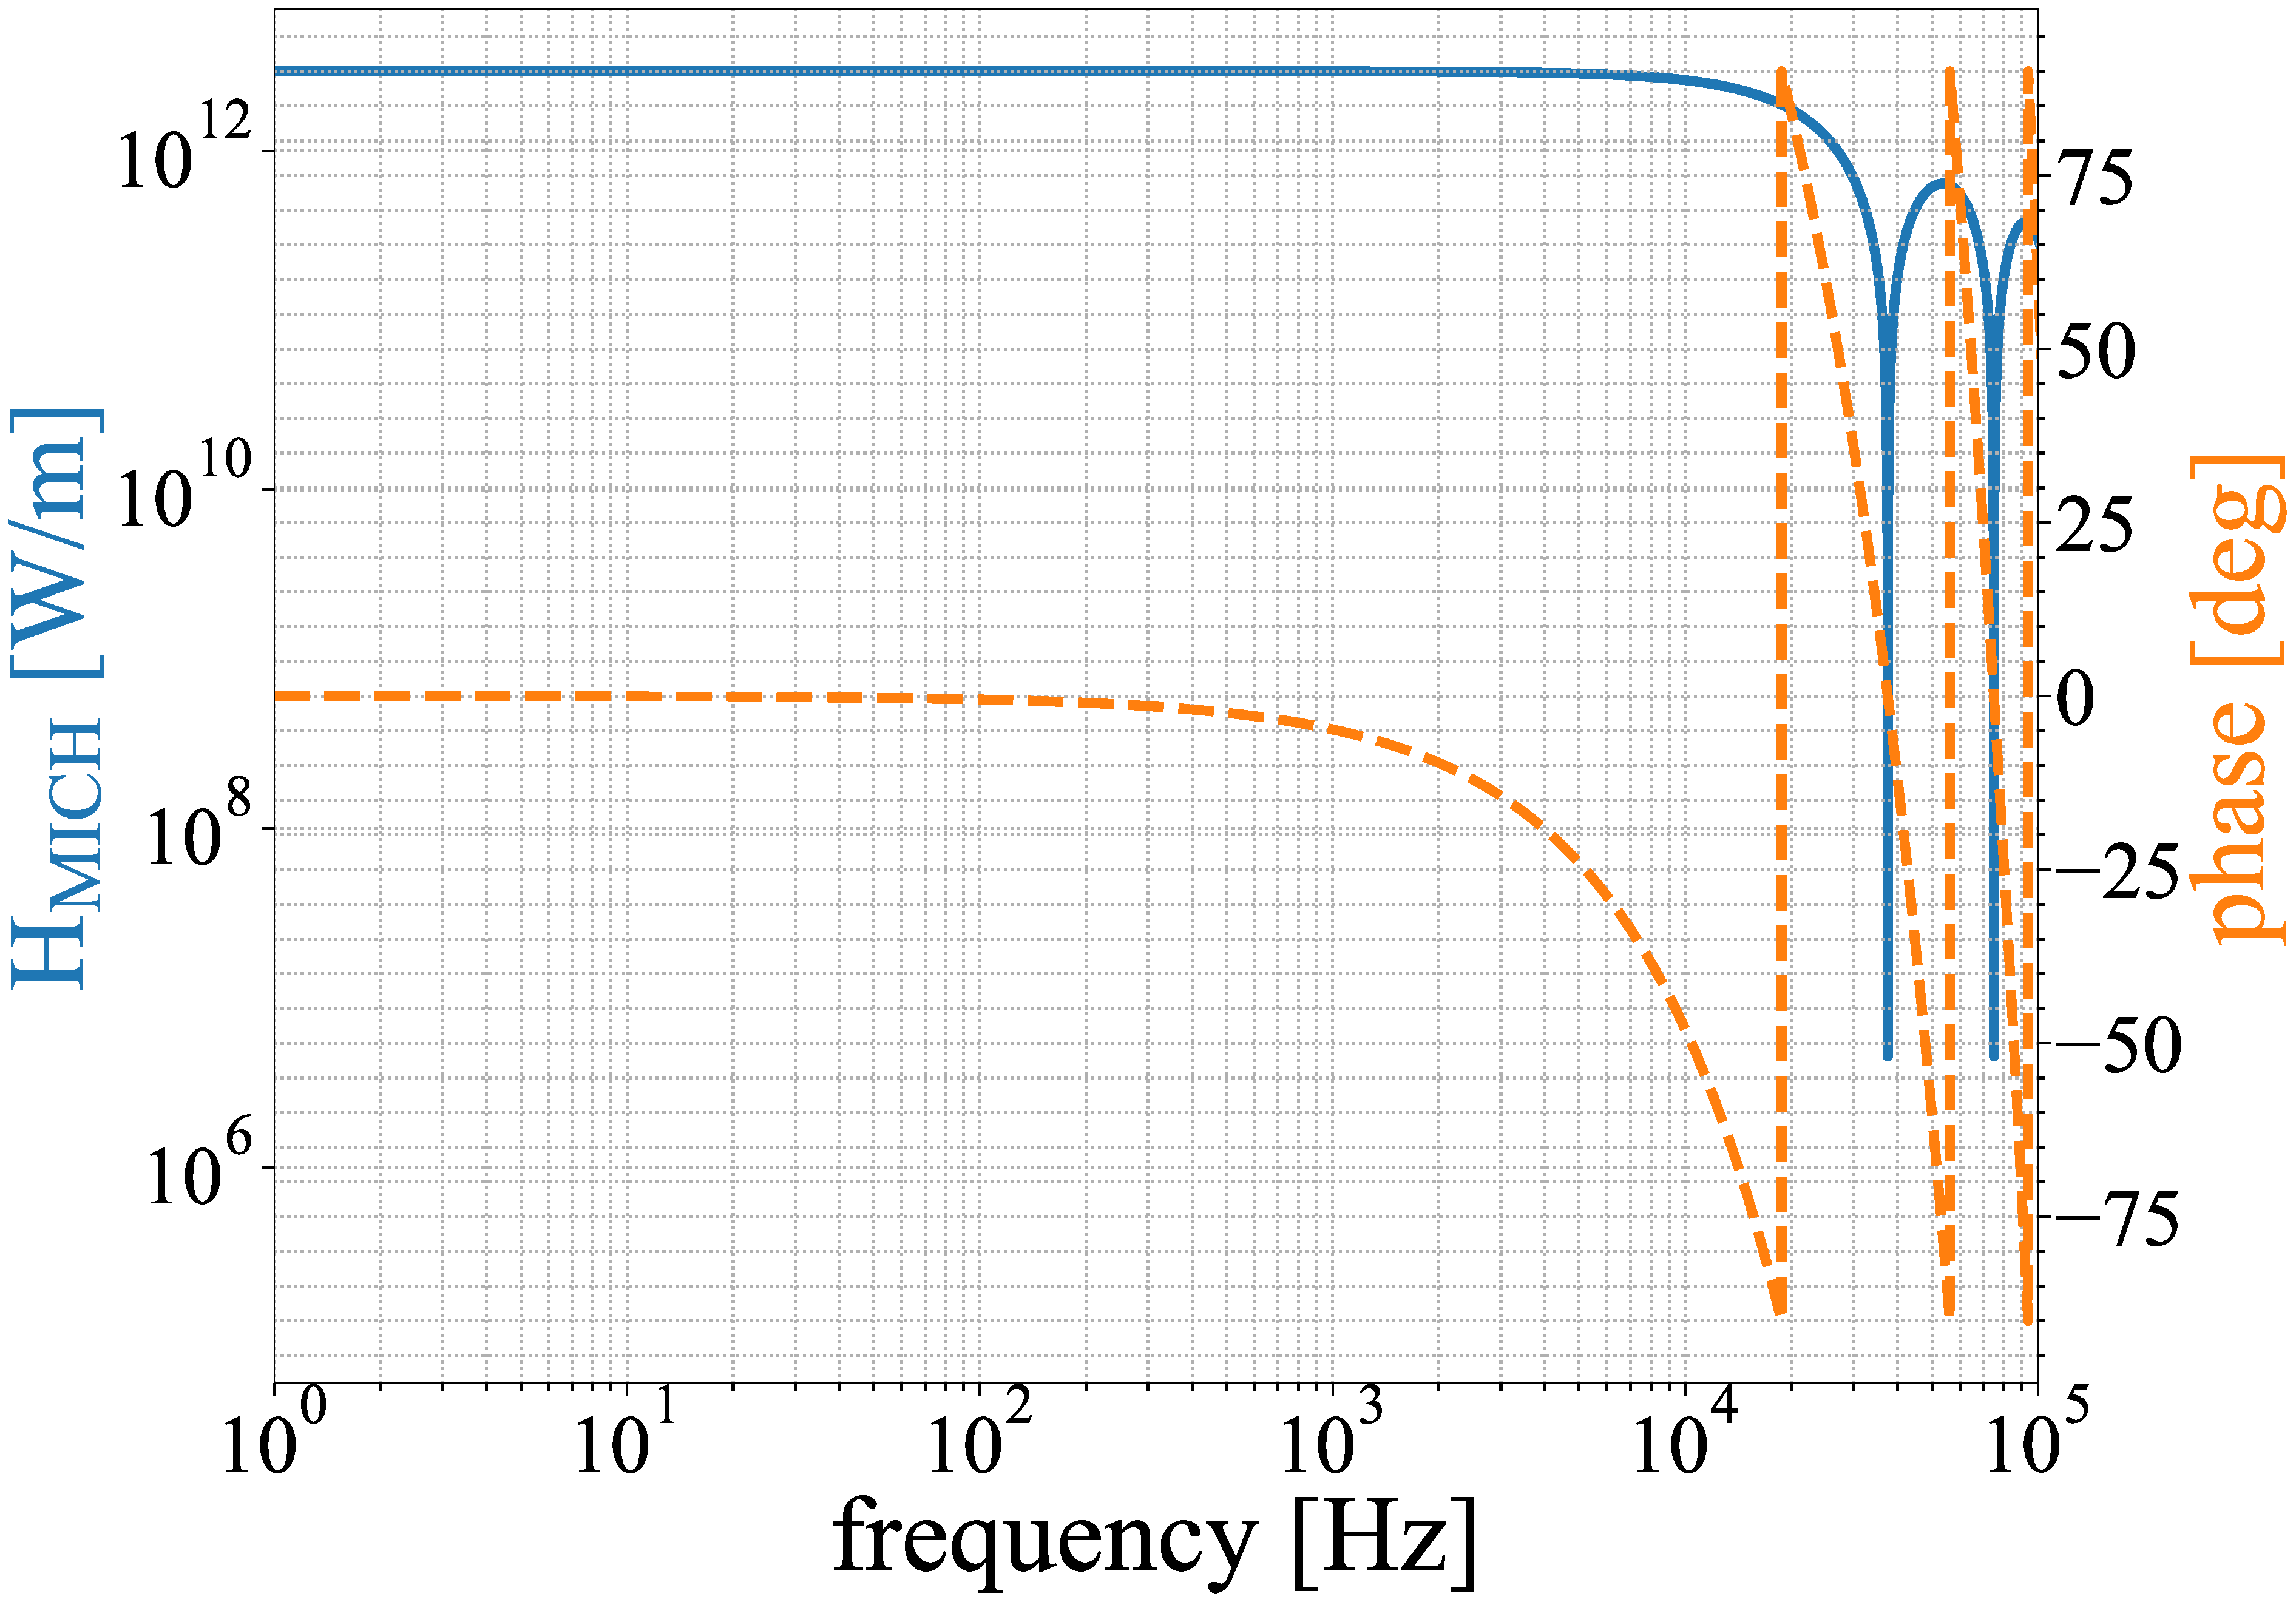
\includegraphics[width=.575\textwidth]{INTRO/mich_fr.pdf}
 	\end{subcaptiongroup}
  	\hfill
	\caption{[Left] A simplified schematic of a Michelson interferometer. [Right] The associated optical transfer function with $H(\omega, \pi/2)$ defining the optical gain of a Michelson interferometer with 4 km long arms and an input power of 25 [W]}
		\label{fig:mich}
\end{figure}
\FloatBarrier

Assuming a 4km arm configuration with 25 Watts input power as indicated in figure \ref{MICH_del_phi} the differential arm response provides a reasonable optical gain with the notches coorelating to an integer number of gravitational wave half periods ($\mathrm{n}\lambda_{gw} / 2$) to the interferometer arm length in such a way that the response is null. Though with sights set on optimizing detection bandwidth for neutron star binaries @ 100 Hz, the basic Michelson optical gain remains insufficient with enhancements required.  

\begin{figure}[ht!]
	\centering
	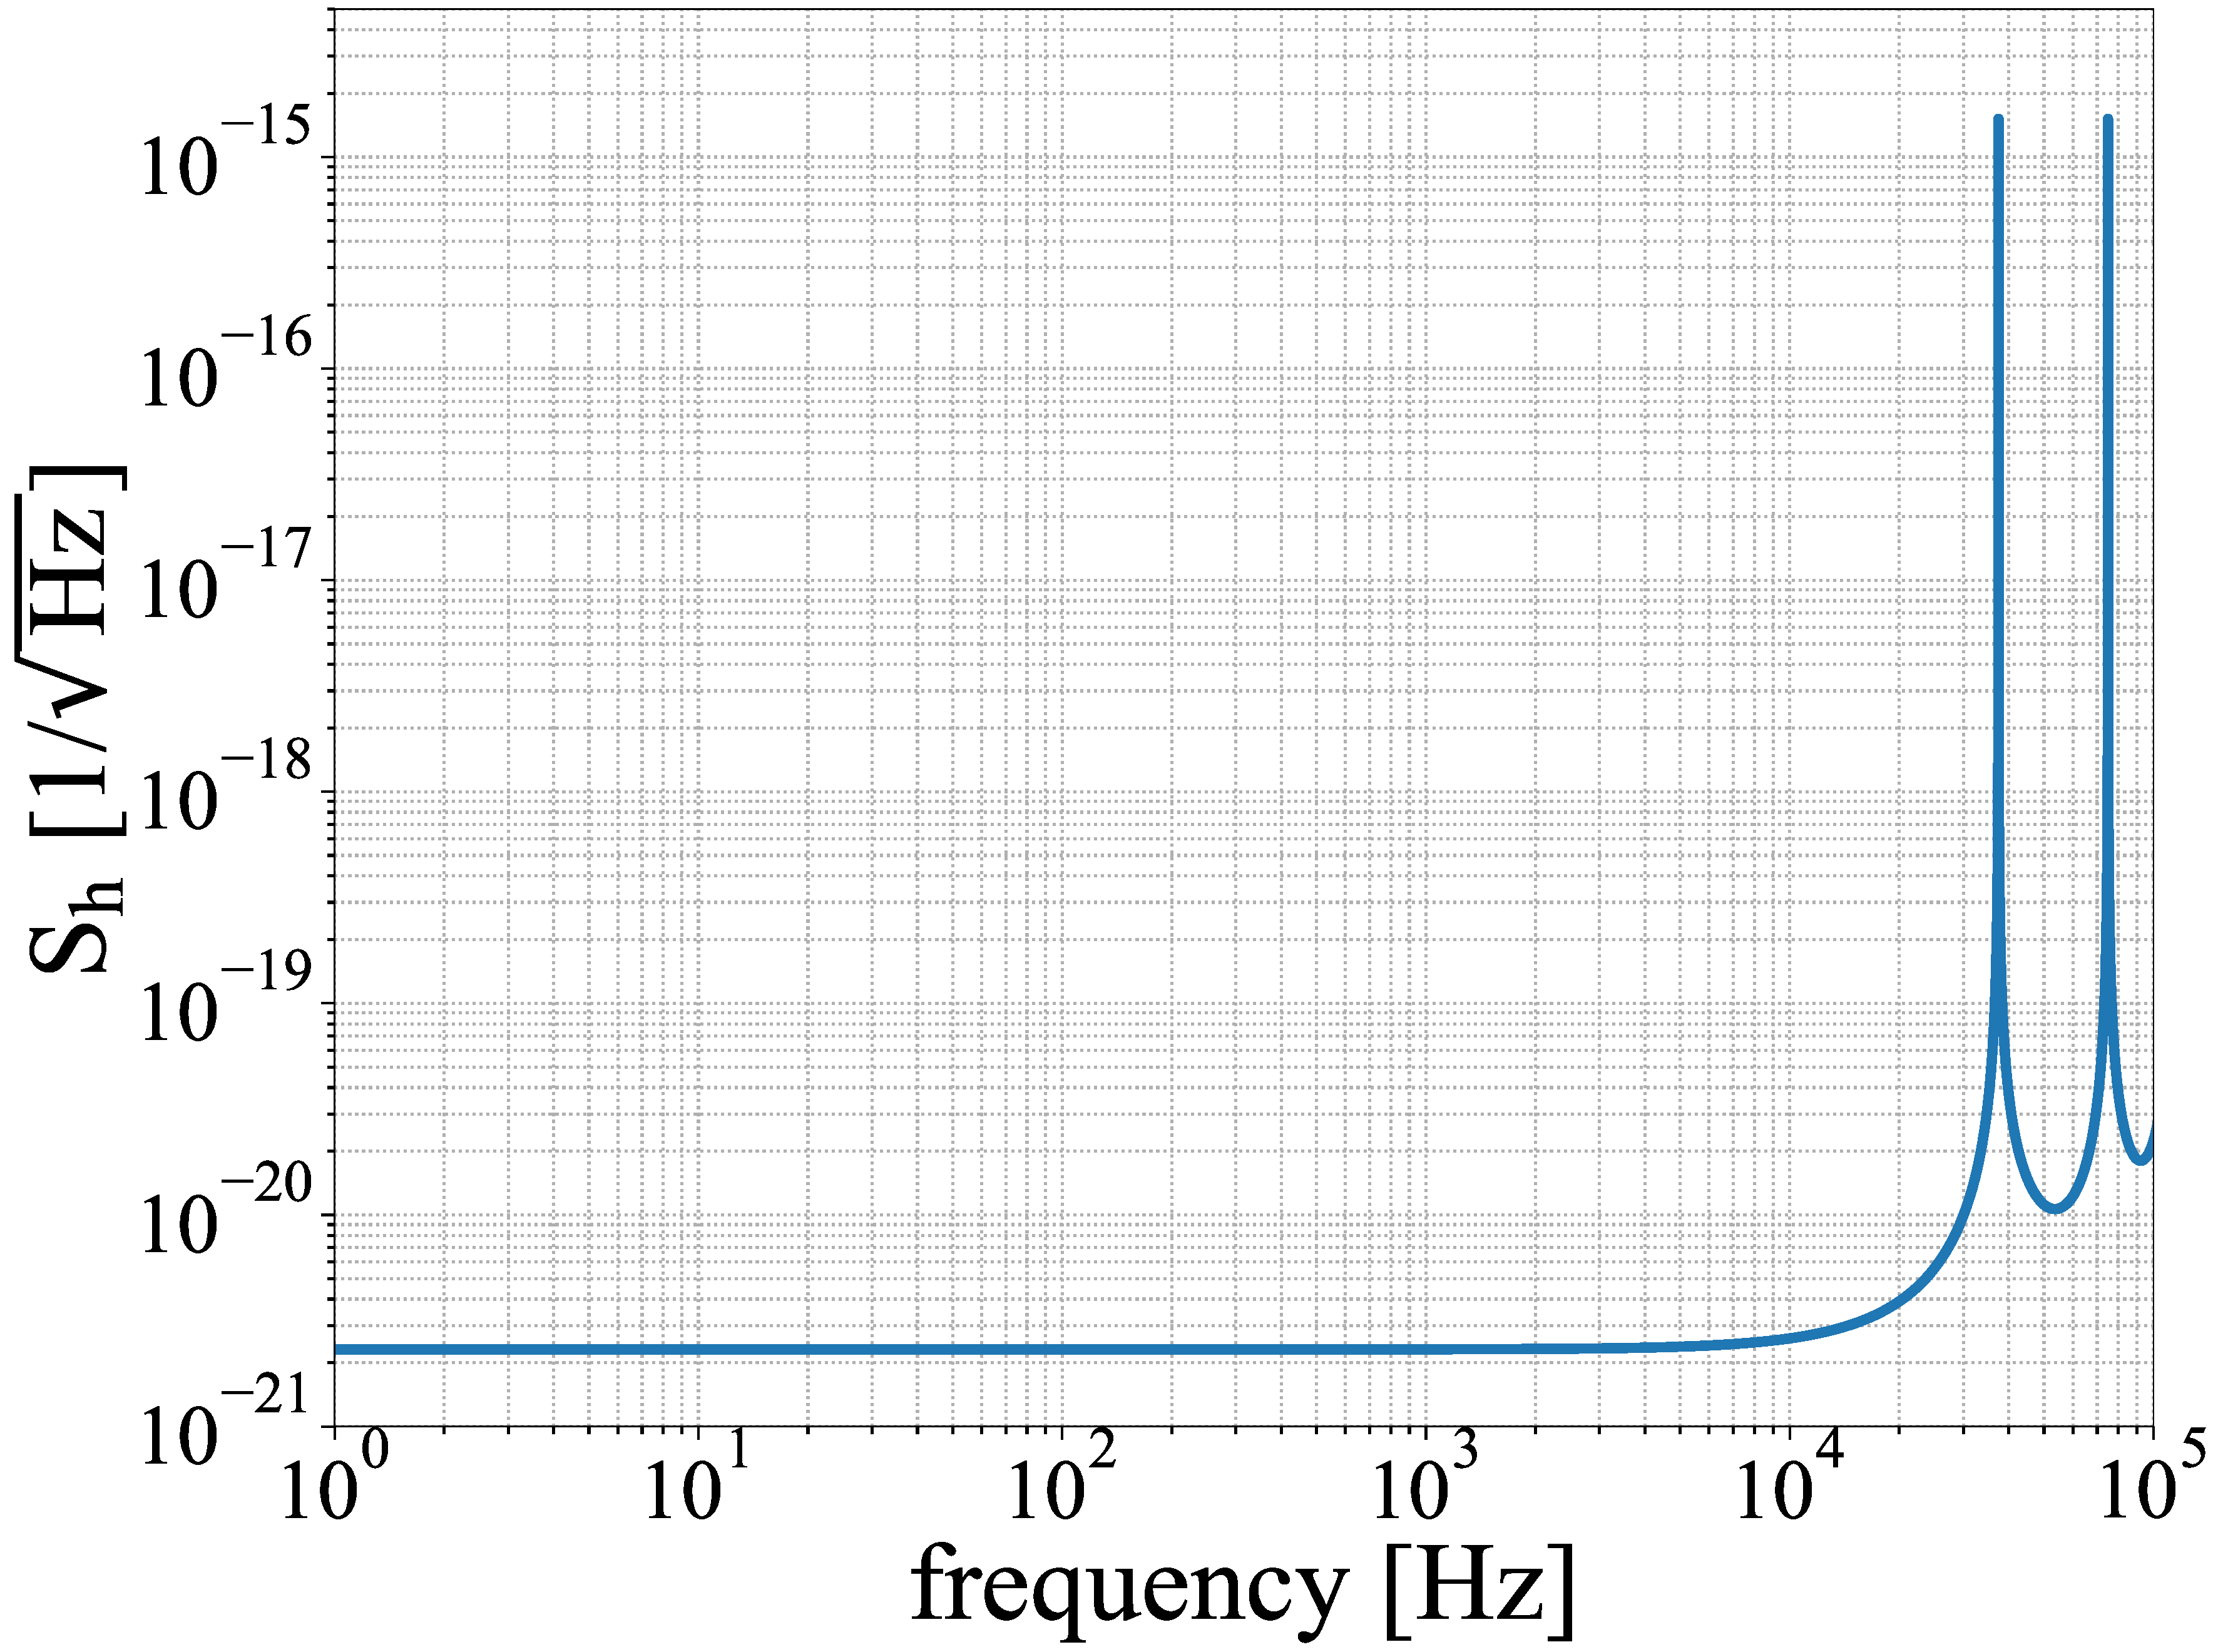
\includegraphics[width=\textwidth]{INTRO/mich_sensi.pdf}
	\caption{The shot noise limited sensitivity ($\sqrt{\hbar \Omega P_\mathrm{in}}$) of a Michelson with 4 km long arms and an input power of 25 [W]. Compared to the apriori estimate of $10^{-21} \; [\frac{1}{\sqrt{\mathrm{Hz}}}]$ the signal to noise (SNR) comes to be unity. The desired confidence is set at a much higher standard with more unquestionable measurements set at SNR = 5.}
	\label{fig:michsensitivity}
\end{figure}

Though with a sensitivity indicated by ~\cite{} [$\mathrm{sensitivity} ~ 1/G_\mathrm{MICH} \approx 10^{-18} \; [\frac{1}{\sqrt{\mathrm{Hz}}}]]$ it still does not reach the requirement to confirm a measurement from CBCs @ 100 Hz ($\approx 10^{-21} \; [\frac{1}{\sqrt{\mathrm{Hz}}}]$.)

\subsubsection{Contrast (Mode Matching Pt. 1)}
As presented, the functional behavior of the simple Michelson is to perform optical autocoorelation; though overly simplified depictions of interferometry suggest operation by periodic planar phasefronts, this doesn't inform the full reality of beam propogation. A standard laser carrier beam mode is represented by the Gaussian beam (TEM00 mode) with wavelength $\lambda$, and propogation axis ($z$):

\begin{equation}\label{eq:gaussian_beam}
E(r) = E_o \frac{\sqrt{[\lambda z_o] / \pi}}{W(z)}e^{-r^2 / W^2(z)} e^{-ikz - ik[r^2 / (2R(z))] + i \zeta(z)}
\end{equation}

Where $E_o$ is a complex field amplitude, $r^{2}/(2(R(z))$ defines transverse coordinates $r = \sqrt{x^{2} + y^{2}}$ on a hemisphere with the ROC of $R(z)$ that defines a surface of uniform phase, $k$ is the wave number, $W(z)$ is the radius from the beam axis that contains $(1-1/e^2) \times 100 \%$ of the integrated beam power, and $\zeta$ is the Gouy phase. An important consideration for any sufficiently long arm length (like that used for LIGO), you are likely to encounter a length constraint from beam divergence if not without a sufficiently large beamsplitter and/or focusing optics. LIGO and most other terrestrial GW detectors manage with curved end mirrors that match / focus impinging wavefronts; symmetrically back propogate them in each arm to maintain optimal interference at the beamsplitter. Mode overlap $\eta$ provides a useful metric of this optimization: 

\begin{equation}\label{eq:mode_overlap}
	\eta = \bigg|\int E_x E_y dA \bigg|^{2} \bigg/ (P_x P_y) 
\end{equation}

Significant length offsets between the arms can contribute to mismatching of the beam mode wavefronts interfering at the beamsplitter. Though an interferometer contrast ($\nu$) measurement may do just as well without more involved beam mode analysis:

\begin{equation}\label{eq:contrast}
	\nu = \frac{P_\mathrm{max} - P_\mathrm{min}}{P_\mathrm{max} + P_\mathrm{min}}
\end{equation}

Operating on a scale from 0 to 1, $\nu \le 1$ can be an indication of : mode mismatch at the beam splitter and/or assymetrical optical loss. From a mode matching perspective $\nu = 1$ represents a mode overlap of $\eta = 100 \%$ (assuming no optical loss).  Though optical losses and aberrations are more often than not asymetrically introduced between the orthogonal beam paths that often limit optimal interference and are indiscriminately accounted for in contrast measurements.  

\subsection{Fabry-P\'{e}rot Michelson (FPMI)}
At the time of the LIGO proposal, constraints (physical and financial) for terrestrial gravitational wave detectors required a compact solution for increasing length (L) of the Michelson arms so to increase the beam phasefront lifetime within the Michelson arms. Two proposed arm folding techniques were considered: the Herriot Delay Line and the Fabry-P\'{e}rot cavity, though ultimately the Fabry-P\'{e}rot cavity is currently the predominent choice.

\begin{figure}[ht!]
	\centering
	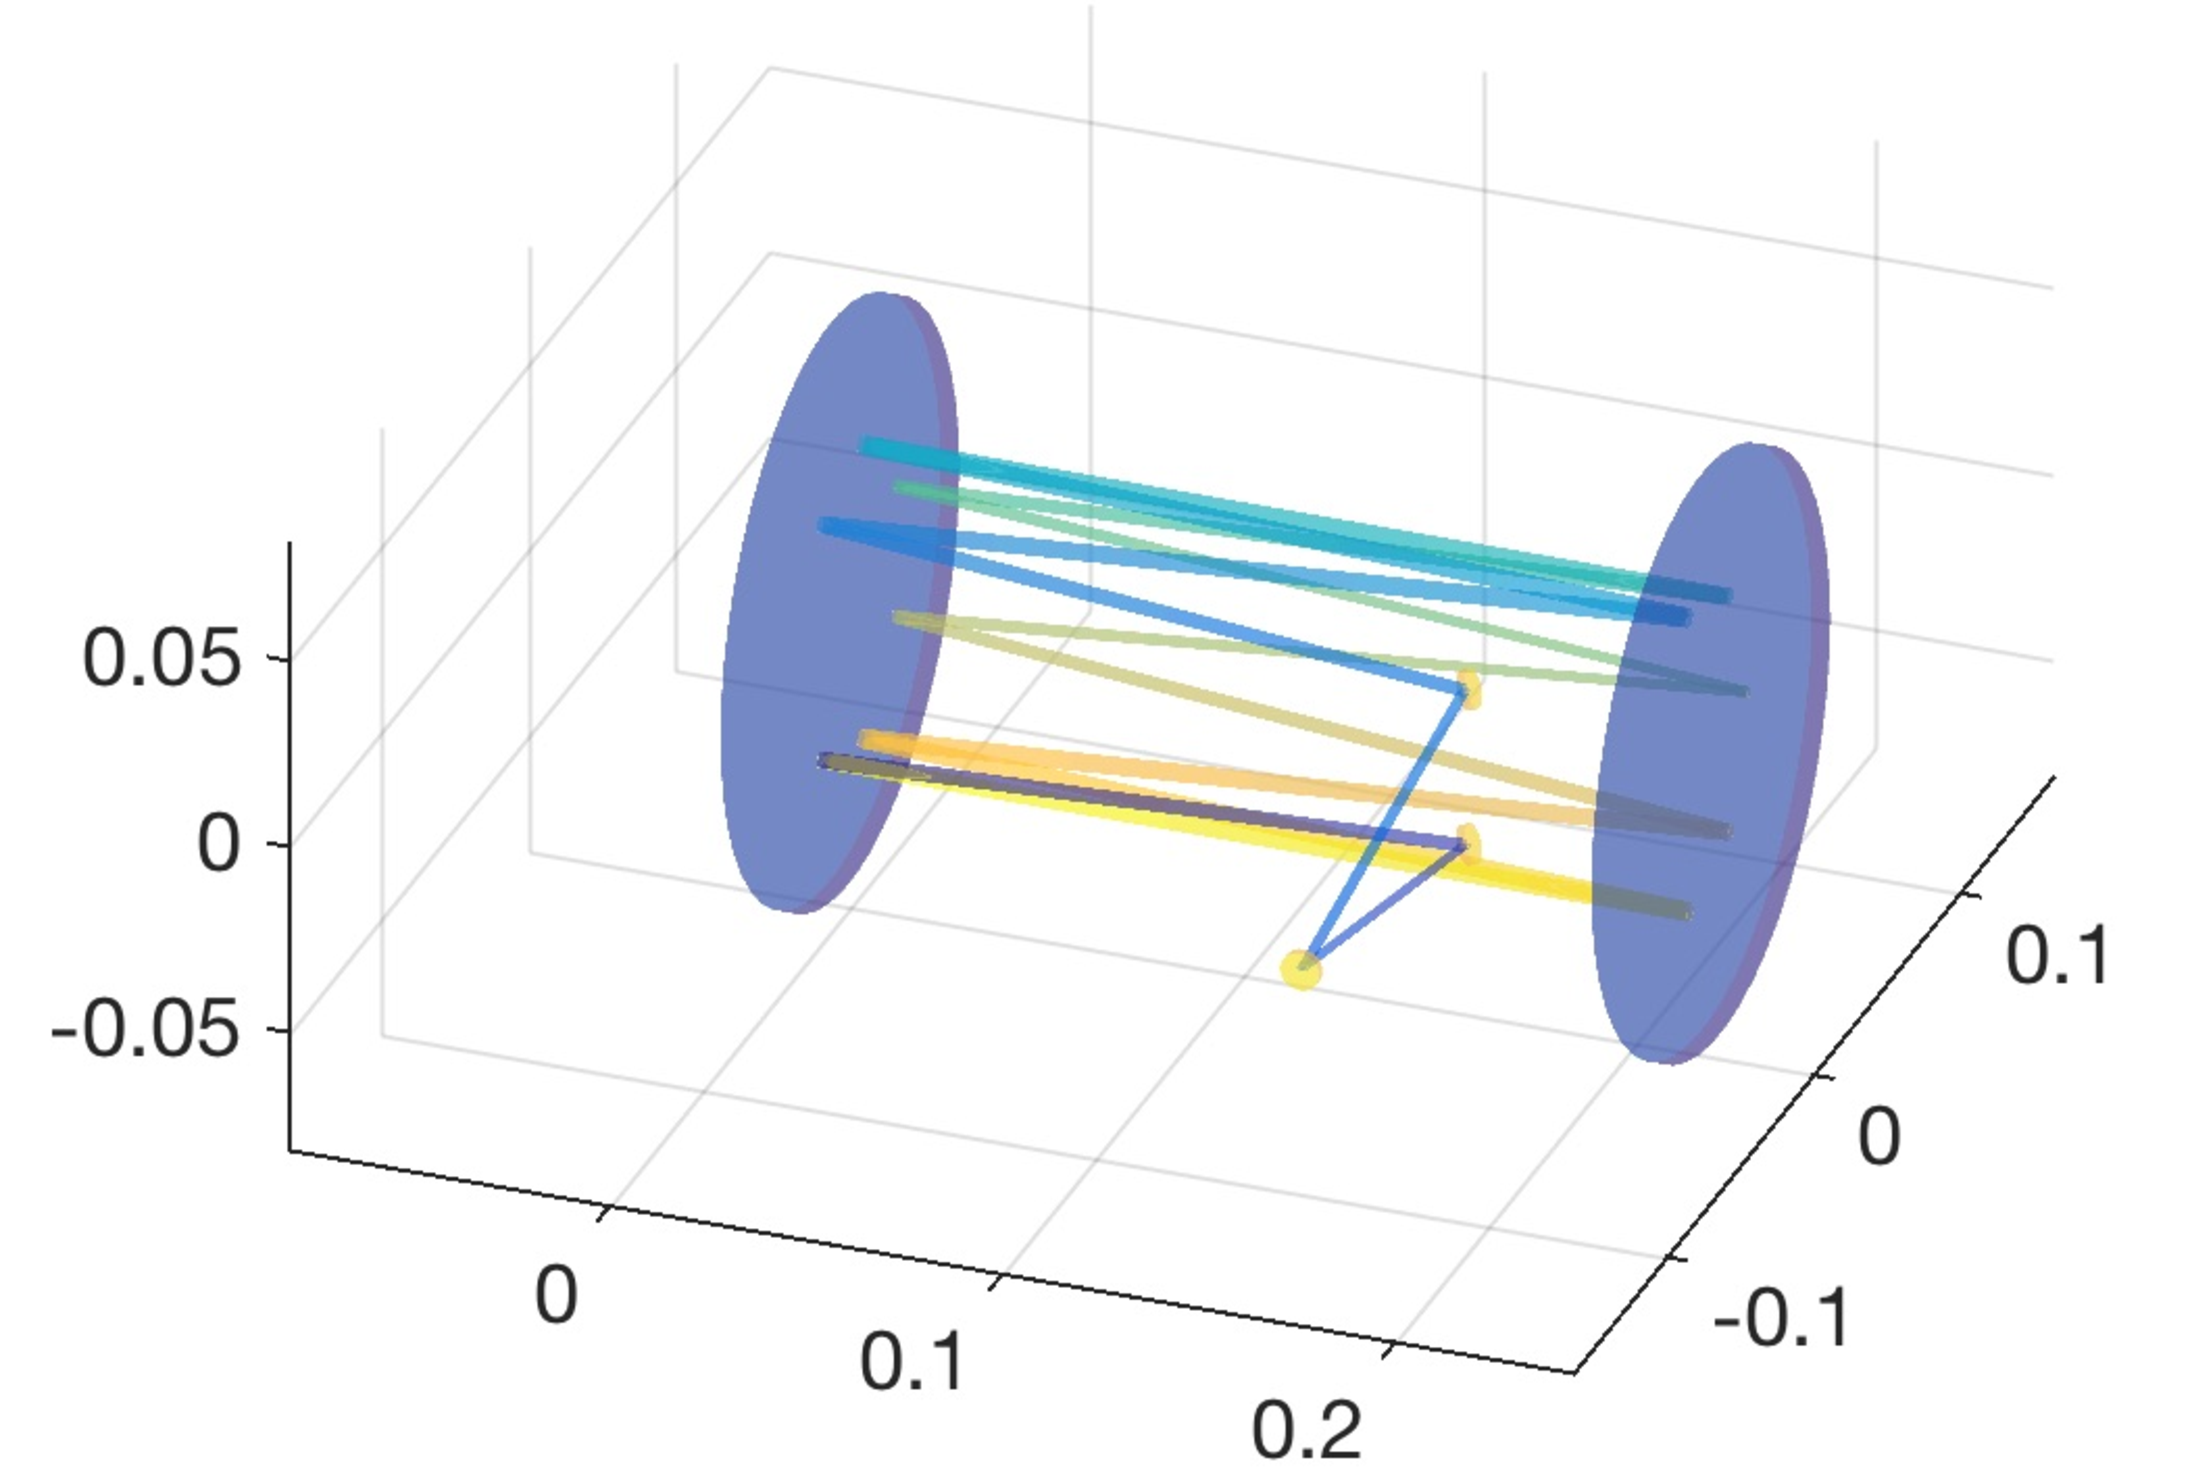
\includegraphics[width=\textwidth]{INTRO/HDL.pdf}
	\caption{A 12 bounce Herriot Delay Line with a small mirror input / output couplers inserted into the beam path.}
	\label{fig:hdl_cav}
\end{figure}


\subsubsection{The Fabry-P\'{e}rot cavity}
\label{section:FPC}
To inform of the folding mechanism, we consider coherent light encountering an optical cavity with input and output mirror transmission and reflection coefficients of $t_1$, $r_1$ and $t_2$, $r_2$ respectively (assuming lossless mirrors $L_1 + L_2=0$).

\begin{figure}[h!]
	\centering
	\includegraphics[width=\textwidth]{INTRO/simple_fp.pdf}
	\caption{Figure of a Fabry Perot Cavity}
	\label{fig:fp_cav}
\end{figure}

Light enters the cavity only after passing the input mirror with the incident field amplitude reduced by the mirror reflection coefficient. Though seemingly not useful, it is with an integer number of wavelengths of the incident laser light between the two mirrors that the circulating beam coherently adds with the input, achieving resonance.  A cavity of length $L$ is comprised of an input coupler ($r_1$,$t_1$) and end mirror ($r_2$, $t_2$) which when configured yield the following effective cavity reflection and transmission coefficients: 

\iffalse that the input and circulating that the photons belonging to a particular phasefront can be experimentally tracked, and lucky for us this is is why we measure interference at the anti-symmetric port. But these benefit with a constant source at the cavity input the phasefronts entering the cavity are superimposed onto the circulating cavity field and, more often than not, add incoherently which can makes this thought experiment seem silly.\fi 

\begin{equation}
	r_c = -r_1 + \frac{t^2_1r_2 e^{-i2kL}}{1-r_1 r_2 e^{-i2kl}}
\end{equation}

\begin{equation}
	t_c = \frac{t_1 t_2 e^{-ikL}}{1-r_1 r_2 e^{-i2kL}}	
\end{equation}

Tuning the positions of mirrors with high reflectivity coefficients and the usage of an infared laser (i.e. $\lambda$ 1064nm) requires strict length tuning and maintenance for resonance ($\leq 1\mathrm{e-}7$ [m]). 

\begin{figure}[H]
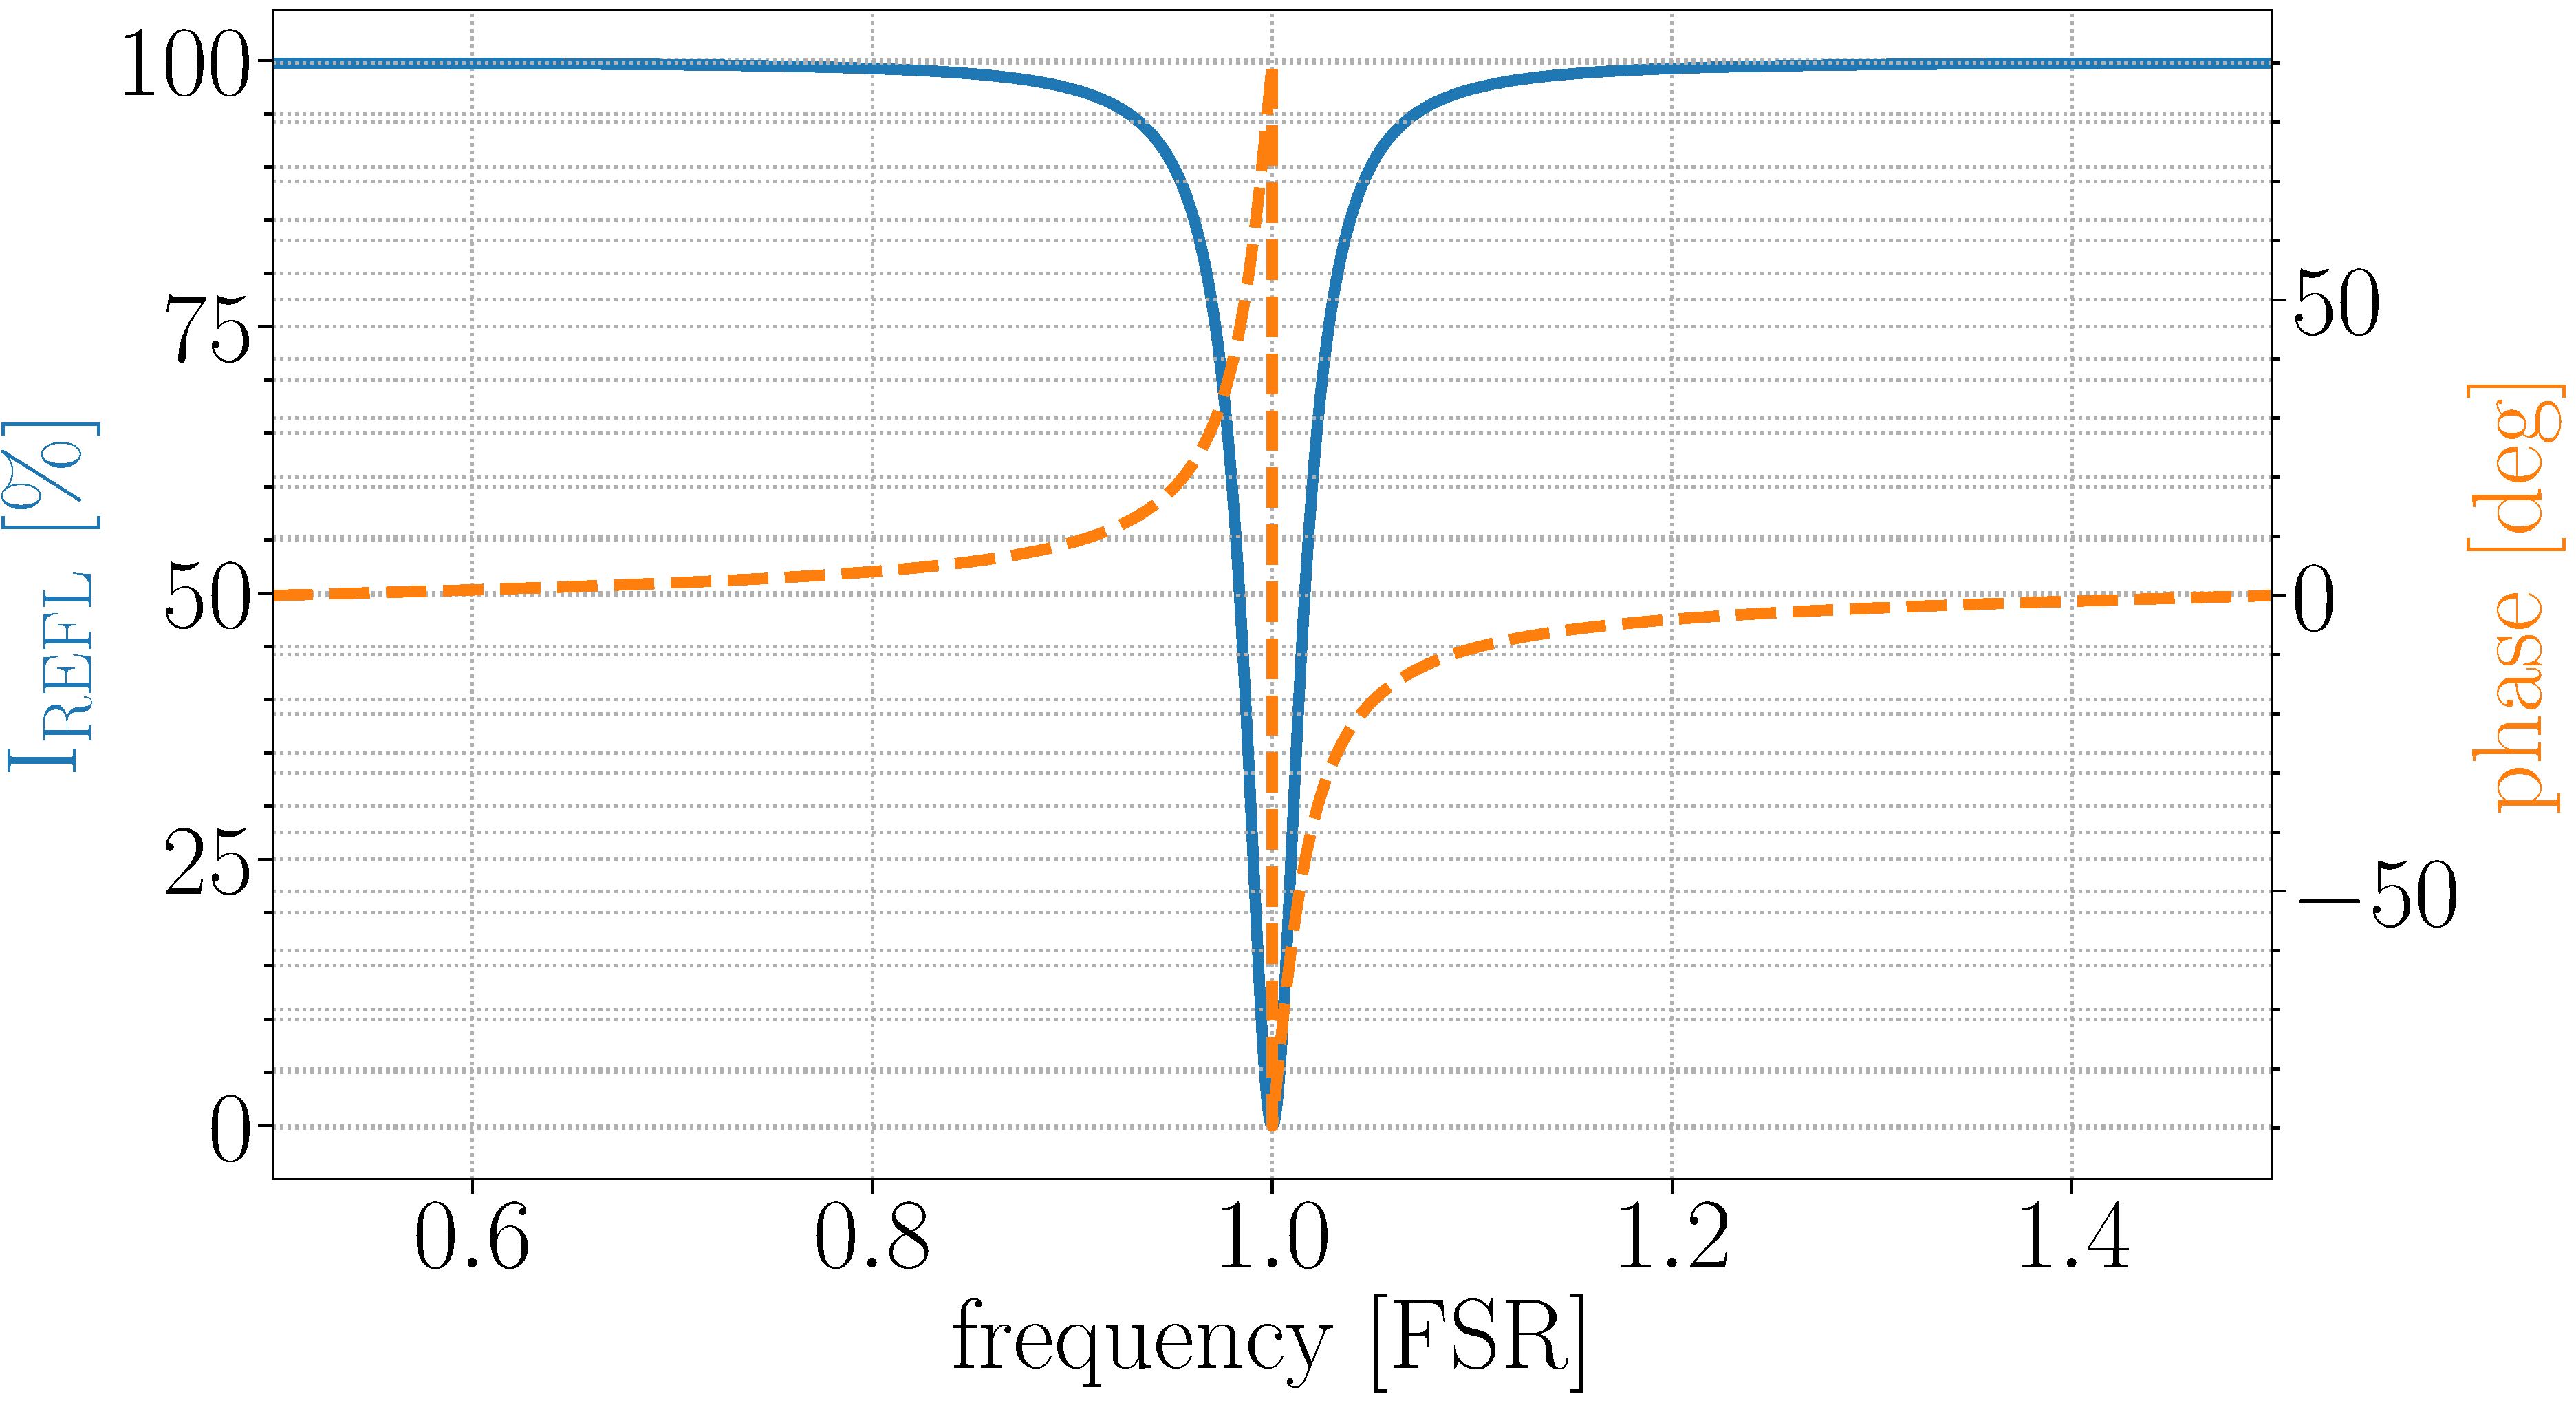
\includegraphics[width=\textwidth]{ALGAAS/REFL_cav_intensity.pdf}
\caption{Reflected cavity intensity (I$_\mathrm{REFL}$) around resonance. The resonance peak full width half maximum is set by mirror reflectivities and is succinctly quantified by the cavity \textbf{finesse} ($\mathscr{F} = \frac{\mathrm{FWHM}_\mathrm{res}}{f_\mathrm{FSR}} = \frac{\pi \sqrt{r_1 r_2}}{1-r_1 r_2}$).}
\label{fig:cav_length_response_DCpow}
\end{figure}

The ratio of the circulating power to the cavity input power is set by the reflectivity paramters of the cavity mirrors; demonstrating the coorelation to how long a given phasefront can remain stored between said mirrors at resonance. This ``cavity storage time" ($\tau_s \appropto L r_1 r_2$) translates as a length elongation with the phasefront travel history encoded in the arrival time of its photons back at the beam splitter.

\begin{figure}[ht!]
  \begin{subcaptiongroup}{\includegraphics[width=.45\textwidth,page=3]{INTRO/ifo_configs.pdf}}
  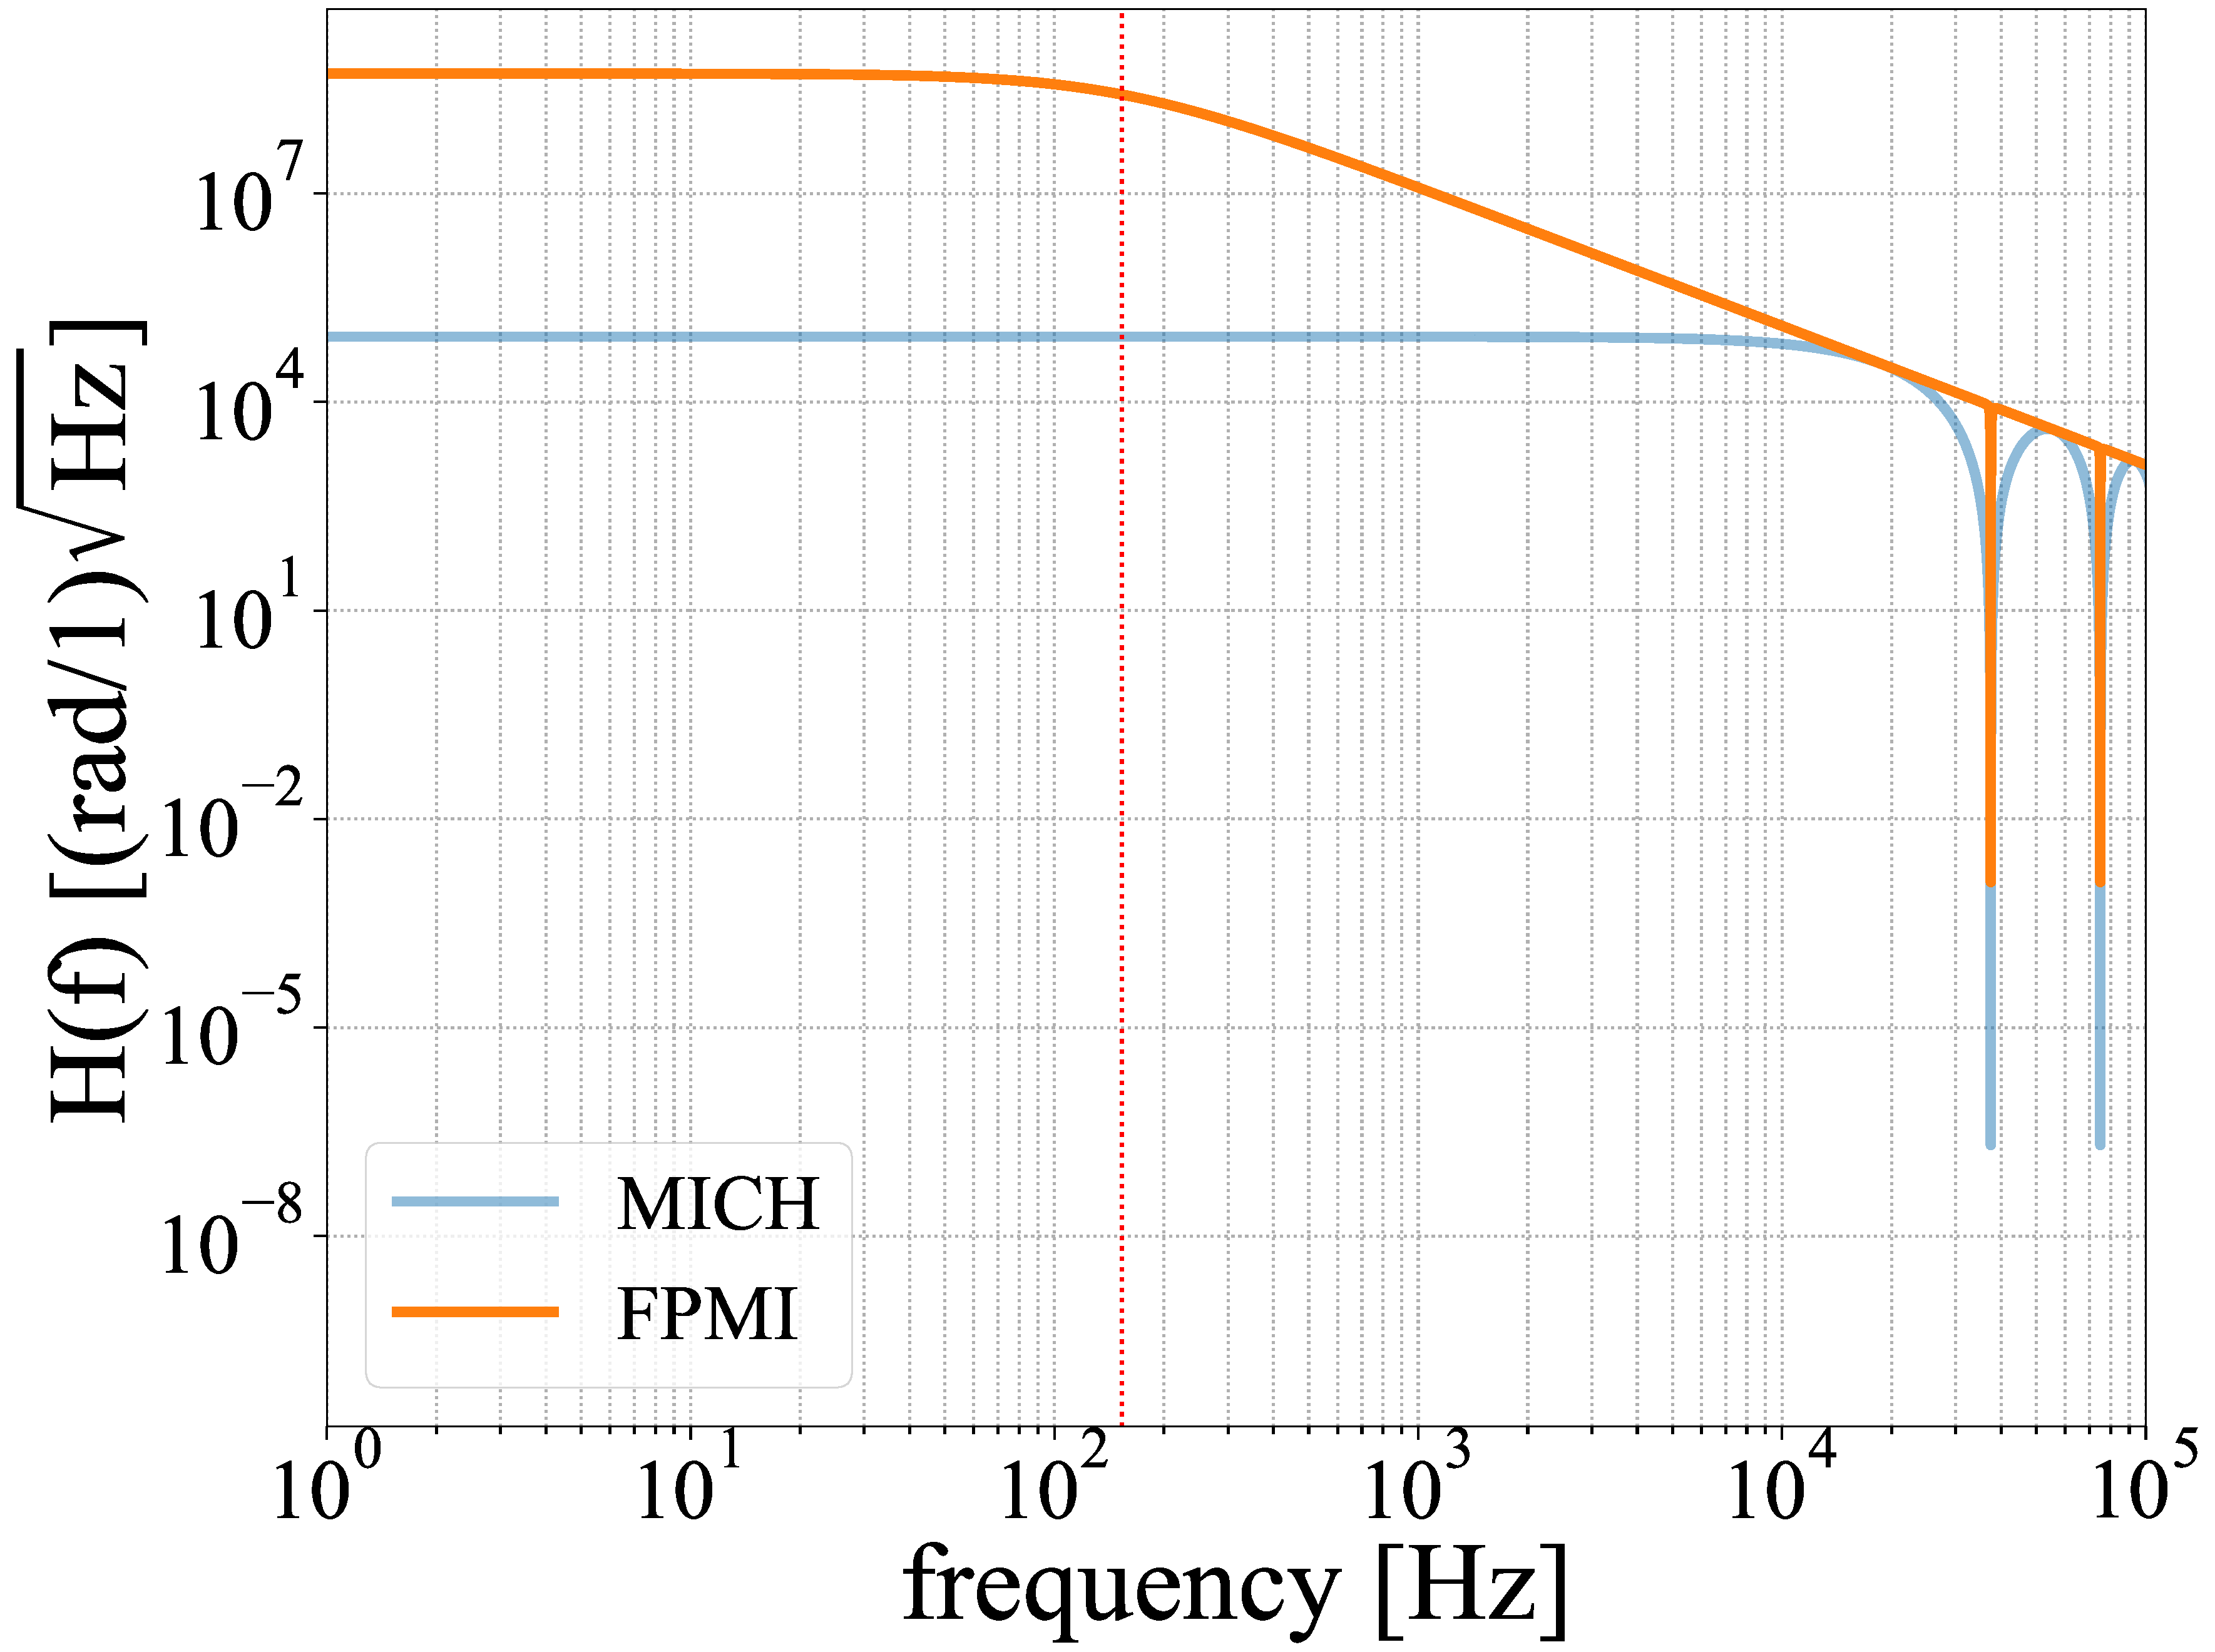
\includegraphics[width=.575\textwidth]{INTRO/fpmi_fr.pdf}
  \end{subcaptiongroup}
  \hfill
  \caption{[Left] The Fabry-P\'{e}rot Michelson optical schema and [Right] an associated optical gain.}
  \label{fig:fpmi}
\end{figure}

\paragraph{``Arm elongation''}

An intuitive analogue of the Fabry-P\'{e}rot's arm elongation capabilities is drawn out when comparing against a computed Delay Line storage time~\cite{saulson2017}:

\begin{equation}
	\tau_s = \frac{L}{c} \frac{r_1r_2}{1-r_1r_2} = \frac{1}{4 \pi \mathscr{F}}
\end{equation}

Advanced LIGO, with its 4km length and approximate finesse of 208 coorelates to a storage time of $382\mu s$, whereas the simple Michelson has an arm storage time of $26 \mu s$. The cooresponding optical gain increase is noted in \ref{fig:fpmi}. 

\begin{equation}
	\mathrm{H_{FPMI}} = \frac{t_1 ^2 r_2}{(t_1^2 + r_1^2)r_2 - r_1} \frac{\mathrm{H_{MICH}}}{1 - r_1 r_2 e^{-2i \omega L / c}}
\end{equation}

It's incredible that simply adding two mirrors can present such detector gain improvement, though in practice the enhancement is contingent upon: 1) maintaining fixed mirror positions within a fraction of the wavelength of the light used and 2) reduction in detector bandwidth. In spite of the narrow mirror displacement requirements, clever experimental techniques like the Pound-Drever-Hall technique allow experimentalists to meet them ~\cite{?}.

\paragraph{Gaussian and Higher Order Mode phasefronts}
Imposing a Gaussian beam to our theoretical two mirror cavity, containing the power of a diverging phasefront between two finite sized mirrors. As mentioned, a simple Michelson with with sufficiently long arms requires focusing a diverging beam by using curved end mirrors to match the beam wavefront. This    The resonance of a gaussian beam requires, one or both of the cavity mirrors to have a finite radius of curvature to match a resonant beam's phasefront \textcolor{red}{see stability criteria}. Though alongside the TEM00 fundamental mode, the paraxial equation (\textcolor{red}{see appendix}) has families of solutions that exist for the aforementioned cavity configuration; these solutions best described by the Hermite-Gauss and Laguerre-Gauss bases:

%%FIGURE: Nonideal interference can result in generating any one of the provided interference patterns. Laguerre-Gauss and Hermite Gauss modes are metrics of mode mismatch and misalignment respectively.

\begin{equation}\label{eq:HG_beam}
	E_\mathrm{n,m}_\mathrm{HG}(x,y,z) = E_o \frac{\sqrt{[\lambda z_o] / \pi}}{W(z)}\mathbb{H}_{\mathrm{n}}\mathbb{H}_{\mathrm{m}}e^{-(x^2+y^2) / W^2(z)} e^{-ikz - ik[(x^2 + y^2) / (2R(z))] + i (1+\mathrm{n}+\mathrm{m})\zeta(z)}
\end{equation}

\begin{equation}\label{eq:LG_beam}
	E_\mathrm{l,m}_\mathrm{LG}(r,\phi,z) = E_o \frac{\sqrt{[\lambda z_o] / \pi}}{W(z)}\mathbb{L}^{\mathrm{l}}_{\mathrm{m}}e^{-\rho^2 / W^2(z)} e^{-ikz - ik[\rho^2 / (2R(z))] - il\phi + i (1+\mathrm{n}+2\mathrm{m})\zeta(z)}
\end{equation}

%%FIGURE: Various mode wavefront solutions with the following caption: ''The various wavefront geometries of the Hermite-Gauss [left] and Laguerre-Gauss modes [right]. Some of these modes are commonly used as error signals used for quantifying the presence of mirror misalignment and mode mismatch."

If it hasn't been clear yet, it certainly will be that the state of cavity resonance is one that is hard to maintain due to its delicate nature.  

\subsection{Dual-Recycled Fabry-Perot Michelson (DRFPMI)}
Recycling mirrors are an extension of the FPMI that exploits otherwise wasted optical power by providing a means of enhancing the optical gain and bandwidth of the instrument. Strategic tuning of mirror coating parameters and positions at symmetric and anti-symmetric ports can incorporate power recycling and signal recycling respectively.

\begin{figure}[ht!]
\begin{center}
\includegraphics[width=\textwidth,page=4]{INTRO/ifo_configs.pdf}
\end{center}
\caption{A simplified Dual-Recycled Fabry-Perot Michelson optical schema}
\label{fig:drfp_michelson}
\end{figure}

\subsubsection{Power Recycling}
When operating a FPMI at a dark fringe, a significant amount of power is reflected back to the symmetric port as mentioned in~\ref{section:FPC} leading to wasted optical power if simply dumped. Placing an additional highly reflective mirror at the symmetric port while maintaining resonance of the carrier to the arms, you can reintroduce (or ``recycle") power back to the arm cavities. A PDH loop is utilized for carrier resonance, and the macroscopic mirror positioning of the PRM is informed by the choice of optical sideband frequency required when applying PDH. 

\begin{equation}
	\mathrm{G_{PR}} = \frac{(1-r_\mathrm{PRM}^2)}{1-r_\mathrm{PRM}[1- (\mathscr{F} \mathscr{L}_\mathrm{RT})/ \pi]}
\end{equation}

With a maximum recycling gain \ref{}: 

\begin{equation}
	\mathrm{G_{PR}} = \frac{\pi}{2 \mathscr{F} \mathscr{L}_\mathrm{RT}} \bigg[ \frac{1}{1- \frac{ \mathscr{F} \mathscr{L}_\mathrm{RT}}{ 2 \pi}} \bigg]
\end{equation}

\subsubsection{Signal Recycling}
As may be inferred, this technique requires a mirror installation at the anti-symmetric port, though with a more nuianced approach than that of power recycling. Placing a partially reflective mirror at the output port it is understood that light leakage coming from the PRFPMI at the anti-symmetric port (caused by differential arm motion) is re-introduced to the arms, but the reflectivity of the new mirror cannot be set too high to avoid attenuating the PRFPMI output. Though detector enhancement only comes after exacting a cost dependent on signal recycling cavity tuning. This cost resides between a trade off of detector bandwidth for increased detector gain or vice versa, with the operating point between the maxima of these two detector characteristics set as a function of the microscopic length (phase) tuning:

\begin{equation}
	\mathrm{H}_\mathrm{DRFPMI} = \mathrm{G}_\mathrm{PR} \mathrm{P}_\mathrm{in} L \Omega \bigg[ \frac{ t_\mathrm{ITM}^2 r_\mathrm{ETM}}{(t_\mathrm{ITM}^2 + r_\mathrm{ITM}^2)r_\mathrm{ETM} - r_\mathrm{ITM}}  t_\mathrm{SRC} \frac{e^{-i 2 \pi L f / c} \mathrm{sin}( 2 \pi f / c)}{ 2 \pi L f } \frac{\mathrm{sin}(\phi_0)}{1- r_\mathrm{SRC}r_\mathrm{ETM} e^{-i 4 \pi L f / c}} \bigg]
\end{equation}

\begin{align}
	t_\mathrm{SRC} & = \frac{t_\mathrm{SRM} t_\mathrm{ITM} e^{i\phi_\mathrm{SRC}}}{1-r_\mathrm{ITM} r_\mathrm{SRM} e^{i2\phi_\mathrm{SRC}}}, \\
	r_\mathrm{SRC} & = \frac{r_\mathrm{ITM} - r_\mathrm{SRM} e^{i2\phi_\mathrm{SRC}}}{1-r_\mathrm{ITM} r_\mathrm{SRM} e^{i2\phi_\mathrm{SRC}}} \\
\end{align}

\begin{figure}[h!]
  \begin{subcaptiongroup}
	  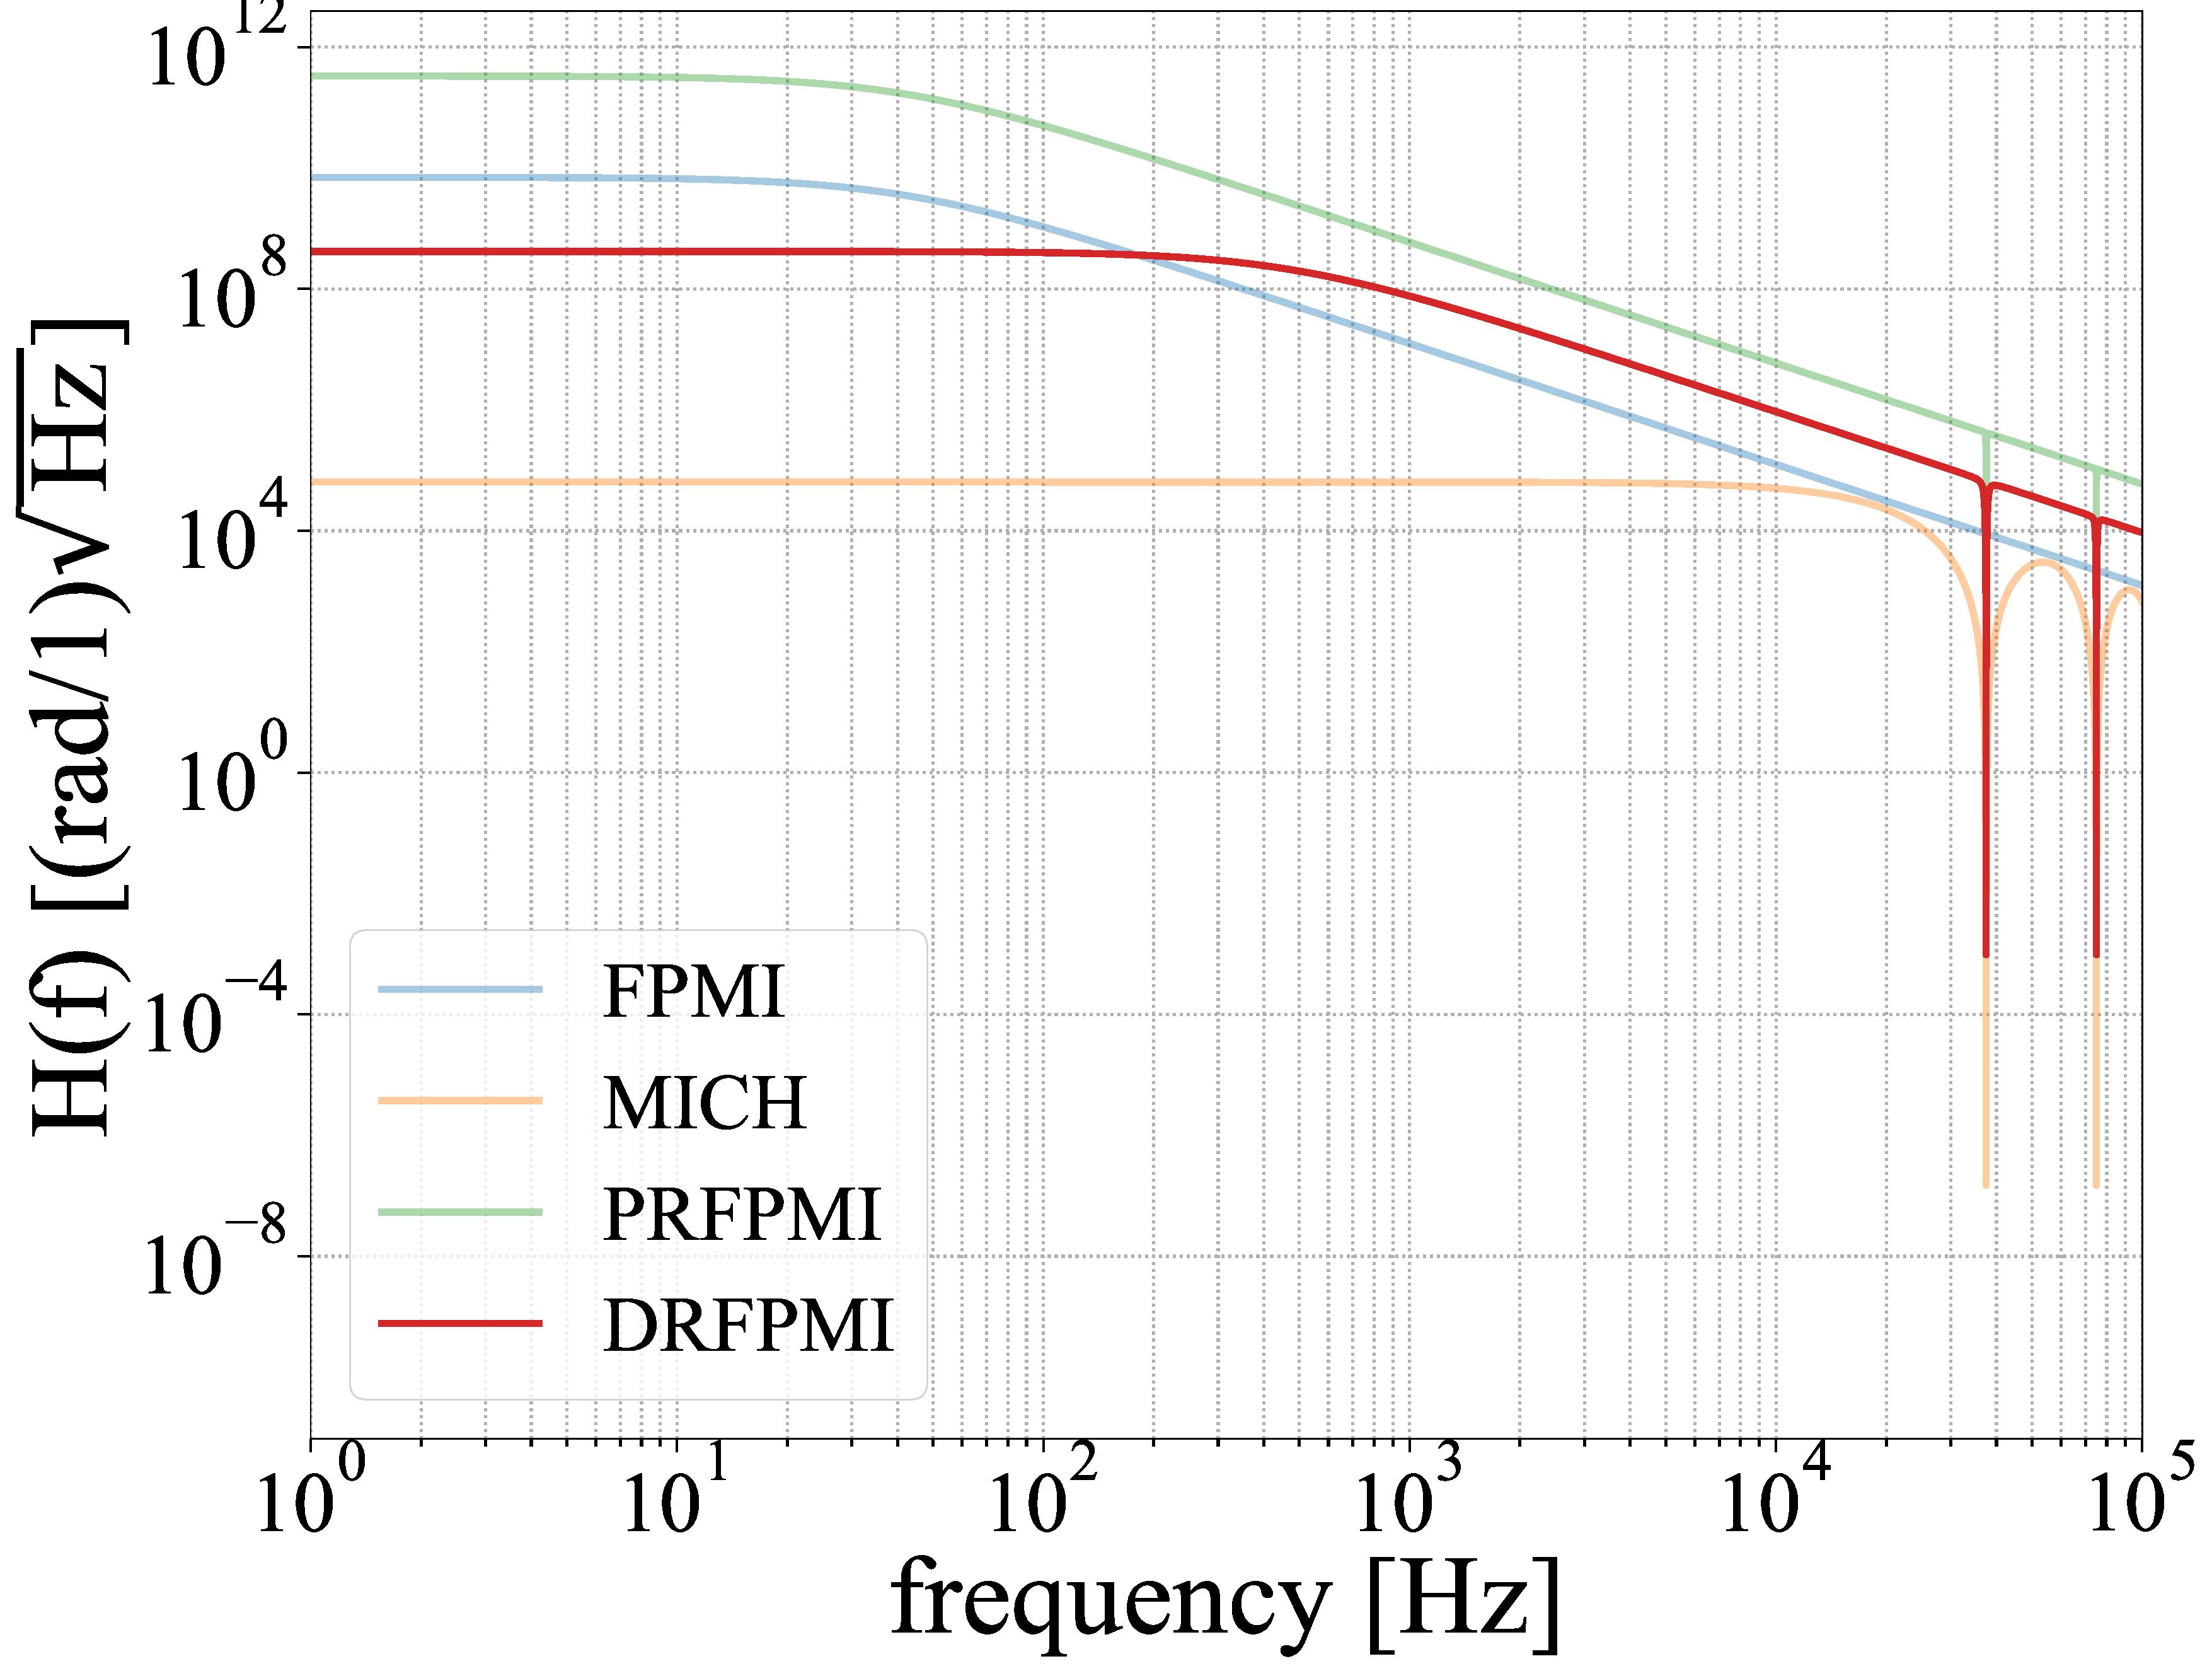
\includegraphics[width=.487\textwidth]{INTRO/drfpmi_fr.pdf}
 	  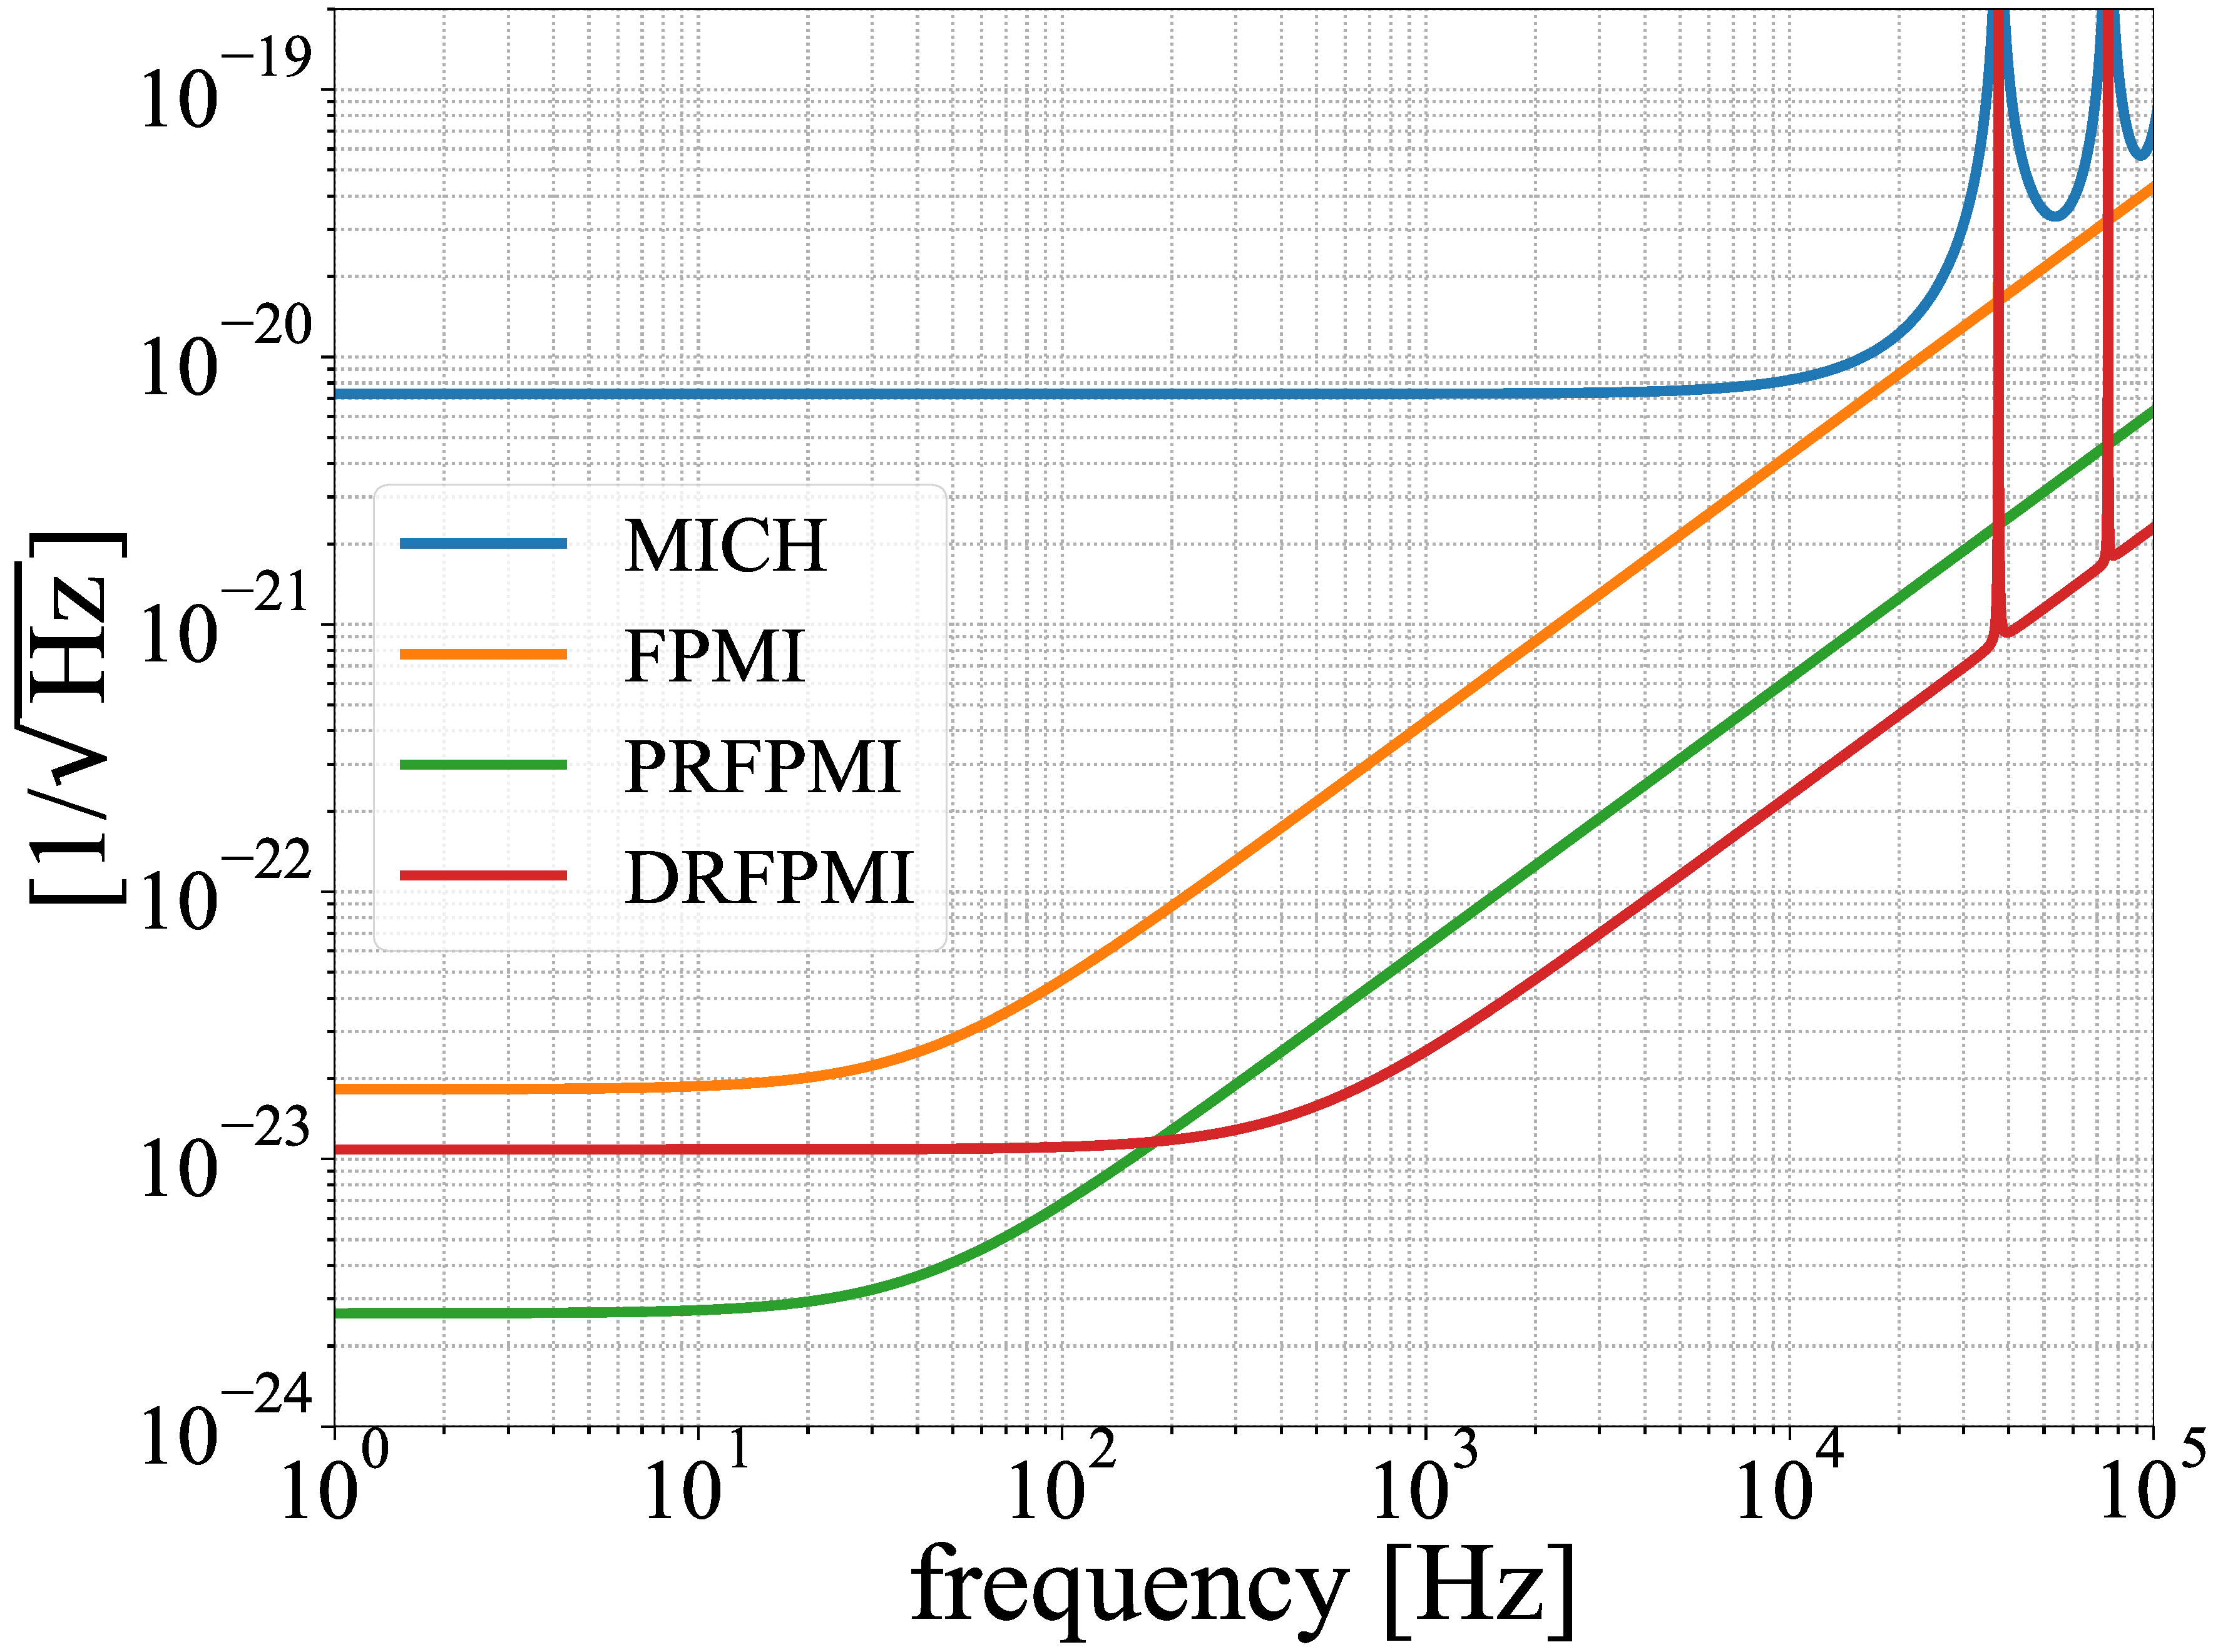
\includegraphics[width=.5\textwidth]{INTRO/strain_compare.pdf}
  \end{subcaptiongroup}
  \hfill
  \caption{[Left] Comparison of all optical gain functions [Right] Coorelated shot noise strain sensitivity.}
  \label{fig:drfpmi_gain_and_strain}
\end{figure}

\section{ALIGO}

\begin{figure}[H]
  \begin{center}
	  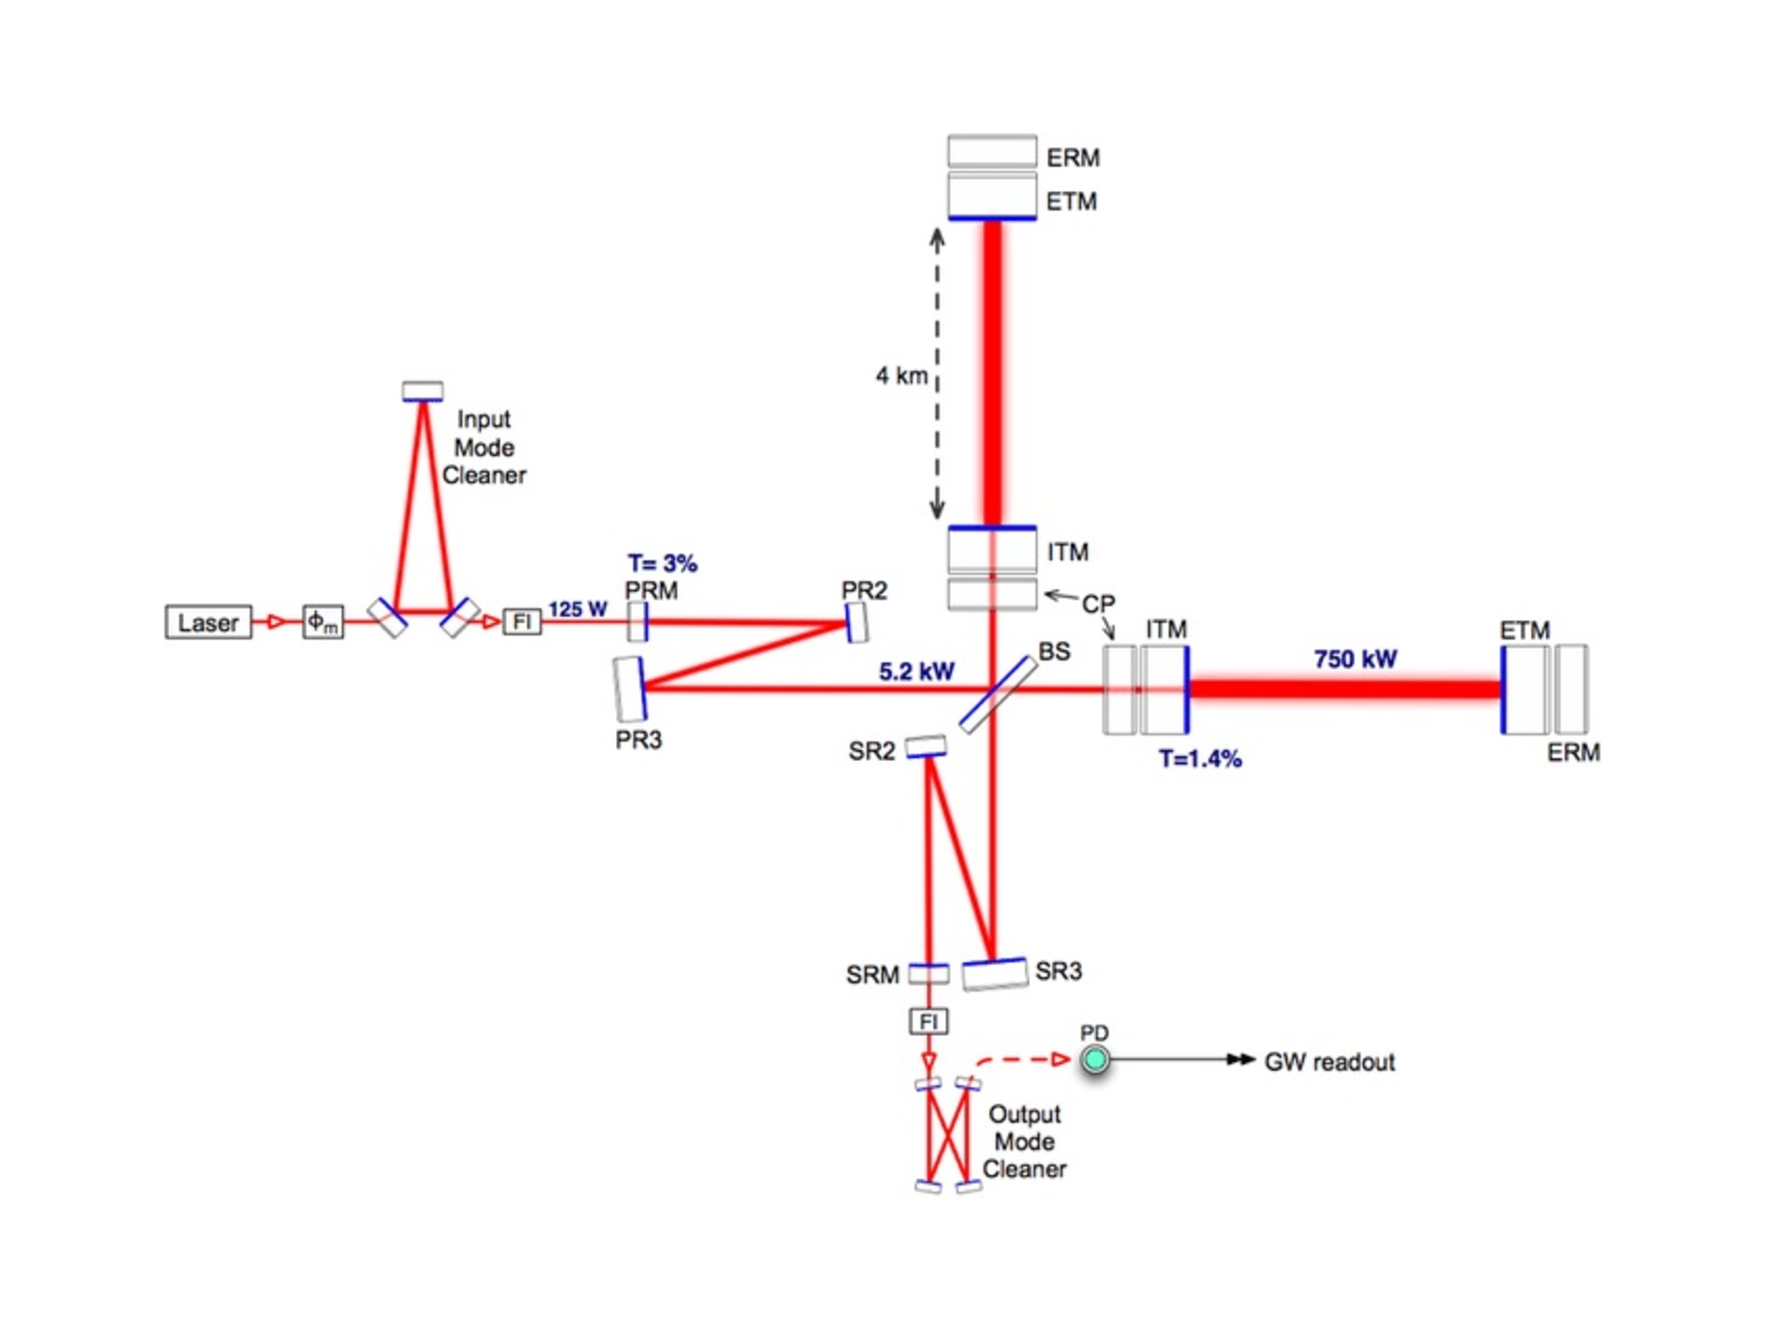
\includegraphics[width=\textwidth]{aligo_config.pdf}
  \end{center}
  \caption{DRFPMI configuration used in ALIGO}
  \label{fig:simple_michelson}
\end{figure}

``Core optics" (Recycling mirrors, Beam splitter, and FP arm cavity mirrors) are suspended with quadruple pendulum suspensions decoupling seismic activity from the mirror positions to as low as a frequency as possible. 

\subsection{Reaching ``Observing Mode"}
The prior discussions still have yet to discuss most of the practical considerations that are required to operate a DRFPMI as a gravitational wave observatory. For the sake of narrowing down the relevance to the body of this work, we discuss more subtle features of the detector: one requires some knowledge of beam optics while the other involves the thermodynamic noise limitation of highly reflective mirror coatings. Alongside this, it is important to know that the studies take place at two very different stages of detector comissoning (One is aimed at comissioning current detectors and the other aims at informing choices to be made for next generation detectors) though both are aimed at increasing gravitational wave detector sensitivity.  The current objective at hand is to inform of these essential criteria for interferometer operations as they pertain to this dissertation. More details on setting up the simple Michelson provides on some of the initial requirements; while the second order is establishing the strict conditions of the Fabry-P\'{e}rot cavities.


\subsubsection{Length Stabilization}
With LIGO's coupled cavity configuration, maintaining mirror positions is imperative. Techniques such as the offset lock (using a DC photodiode to measure the transmitted, reflected, or circulating power within a linear and slightly off resonance point) \cite{} and the Pound-Drever-Hall technique (see \ref{subsubsec:pdh} ) are used to maintain cavity length stabilization. Stabilizing cavity lengths to configure the detector into a highly sensitive differential arm sensor is a process that is worthwhile understanding with more ample discussions ~\cite{Mullavey:12}.


%So far, we've discussed light and phase fronts without addressing geometric
%constraints when using Gaussian laser light. We consider a general complex
%Gaussian beam mode propogating along the beam axis ($z$) with wavelength
%$\lambda$.

%\begin{equation}\label{eq:gaussian_beam}
%E(r) = E_o \frac{\sqrt{[\lambda z_o] / \pi}}{W(z)}e^{-r^2 / W^2(z)} e^{-ikz - ik[r^2 / (2R(z))] + i \zeta}
%\end{equation}
%
%Where $E_o$ is a complex amplitude, $r = \sqrt{x^2 + y^2}$ defines the transverse beam coordinates, $k$ is the wave number, $W(z)$ is the beam width, $R(z)$ is the beam radius of curvature, and $\zeta$ is the Gouy phase.

Derived from the paraxial approximation of the Helmholtz equation, this field is not the only solution for optical cavities. Alternative higher order mode (HOM) solutions are commonly present and are expressed in terms of two mathematical bases: the Hermite-Gauss and Laguerre-Gauss modes. These HOMs are more often than not power parasites when attempting to only sense displacement Fabry-P\'{e}rot cavities and are a symptom of altered cavity geometry; though a virtue of the lost power is its utility as an error signal for sensing and actuation schemes. This is what is what is accomplished with an alignment sensing and control (ASC) system and a thermal compensation system (TCS) for mode matching actuation.

%%FIGURE: ALIGO Sensor and Actuation schema

\subsubsection{Alignment sensing and control}

\begin{figure}[H]
    \begin{center}
    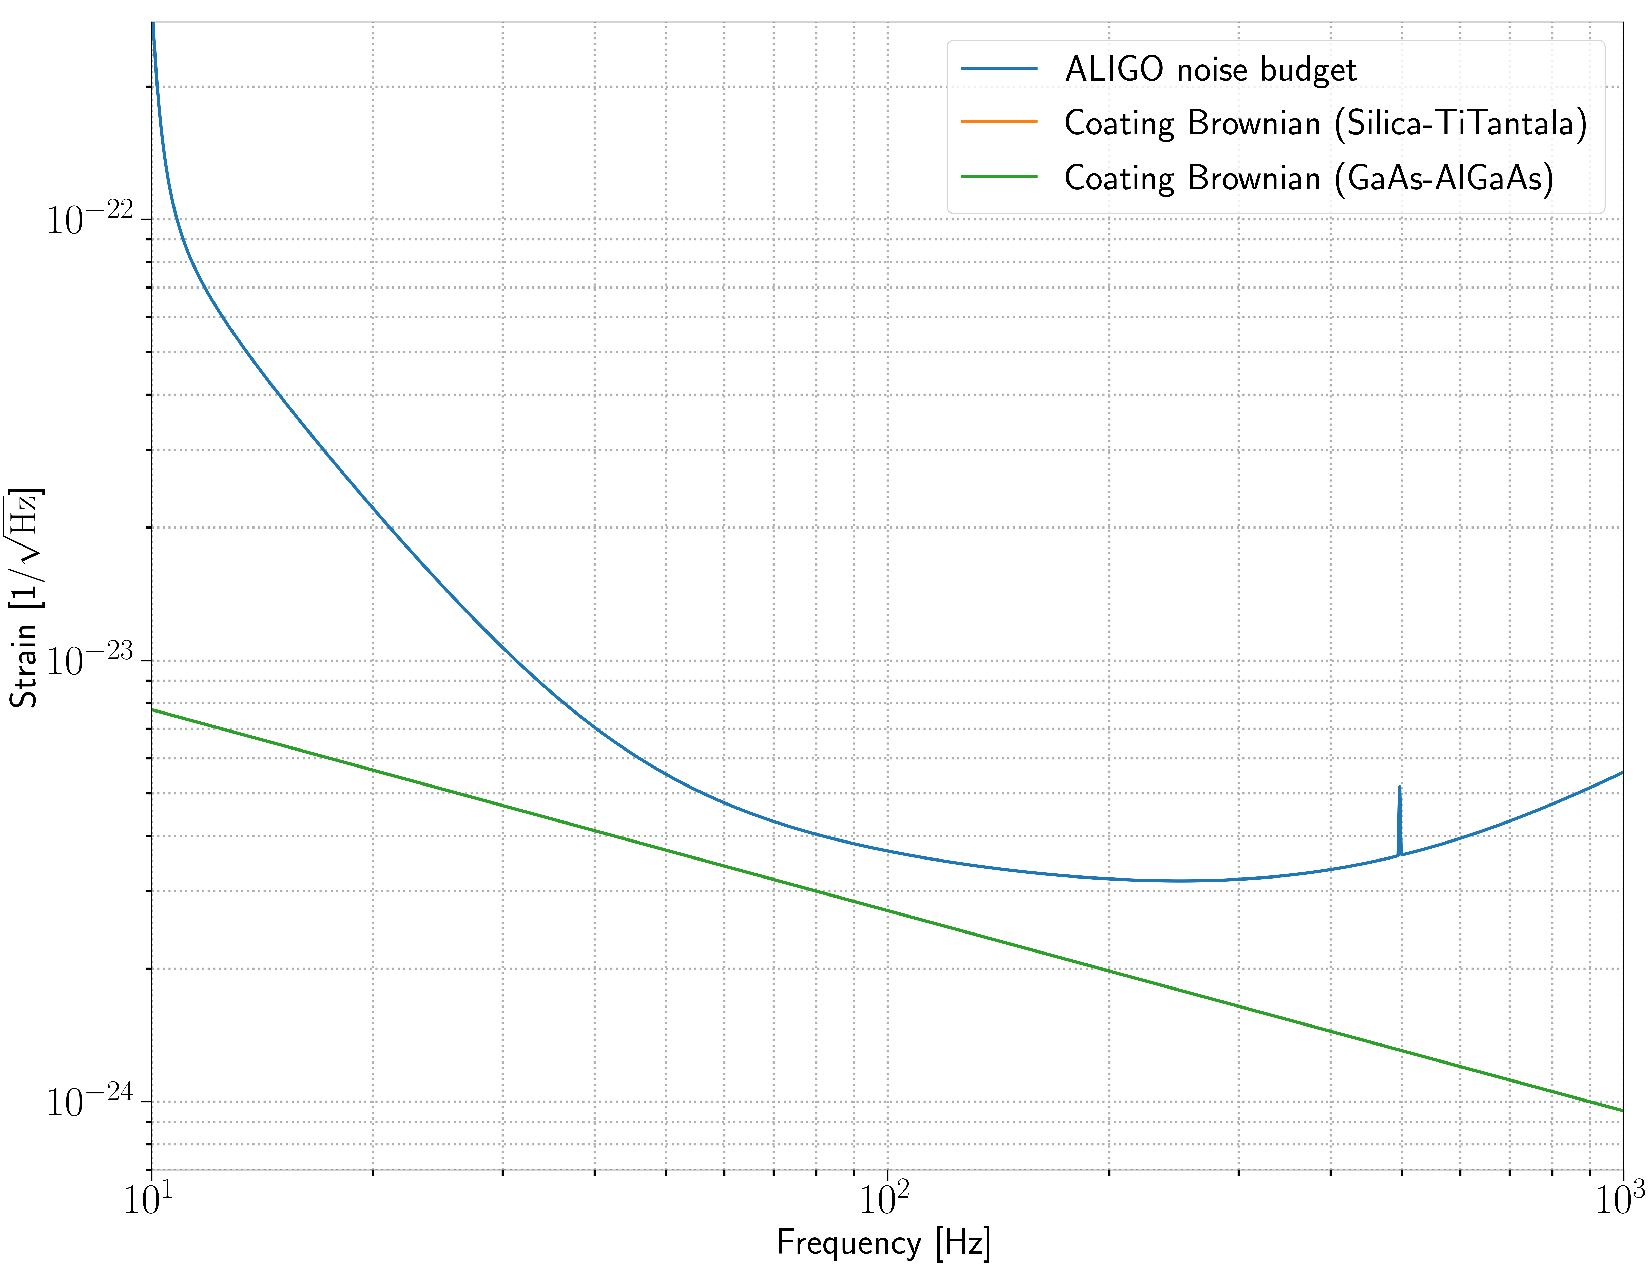
\includegraphics[width=.5\textwidth]{ALGAAS/aligo_nb_plus_cbn.pdf}
    \end{center}
    \caption{A misaligned Fabry-P\'{e}rot cavity scatters circulating light into higher order Hermite-Gauss modes.}
    \label{fig:HGLGmodes}
\end{figure}

\begin{equation}
	E_{n,m}(x,y,z) = E_o \bigg[ \frac{W_o}{W(z)} \bigg] H_n \bigg[ \frac{\sqrt{2}x}{W(z)} \bigg] H_m \bigg[ \frac{\sqrt{2}x}{W(z)} \bigg] e^{-(x^2 + y^2)/W(z) - ikz - ik[(x^2 + y^2)/(2R(z))] + i(n + m + 1)\zeta(z)}
\end{equation}

Even with state-of-the-art ground motion isolation for terrestrial gravitational detectors using quadruple stage pendula and high mass mirrors, current gravitational wave detectors still suffer from occasional misalignment and require sensing and feedback loops to meet mirror alignment requirements.

\subsubsection{Mode Matching}
For Gaussian beams, there are further requirements of macroscopic mirror positions and radius of curvatures to maximize resonant power in the fundamental (TEM00) mode. Failure to plan and maintain these conditions sucessfully results in a mismatch of the beam mode to the cavity mode, scattering power into higher order Laguerre-Gauss modes.  

\begin{equation}
 E_{n,m}(\rho, \phi, z) =  E_o \bigg[ \frac{W_o}{W(z)} \bigg] H_n \bigg[ \frac{\rho}{W(z)} \bigg]^2 L^n_m \bigg[ \frac{\sqrt{2}\rho^2}{W^2(z)} \bigg] e^{-\rho^2/W(z) - ikz - ik[\rho^2/(2R(z))] - jn \phi + i(n + 2m + 1)\zeta(z)}
\end{equation}

Even with ultra-low absorption HR mirror coatings and fused silica substrates, circulating power is estimated to reach $\geq$ 200 kW, distorting the radius of curvatures of the arm cavity mirrors by ? m; which can introduce significant optical loss due to mode mismatch (esp. for coupled cavities). And as a DRFPMI like aLIGO approaches designed sensitivity, instances of mode mismatch can be a two-fold threat with optical loss to higher order modes also impacting the ability to produced squeezed light states~\cite{}. The solution implemented in aLIGO as of O3 to sense mode mismatch consists of hartmann wavefront sensors (HWS) with 800 nm and 833 nm probe beams providing real-time mirror lensing / surface distortion data while actuation comes in the form of induced thermal actuation on mirrors throughout the interferometers with particular focus on the arm cavity mirrors. The thermal actuation of the core optics comes in two varieties: a CO2 laser actuator impinging upon a pre-installed fused silica compensation plate (CP) for positive lens actuation and an annular ring heater for negative lens actuation \cite{}. 

%\begin{figure}[H]
%	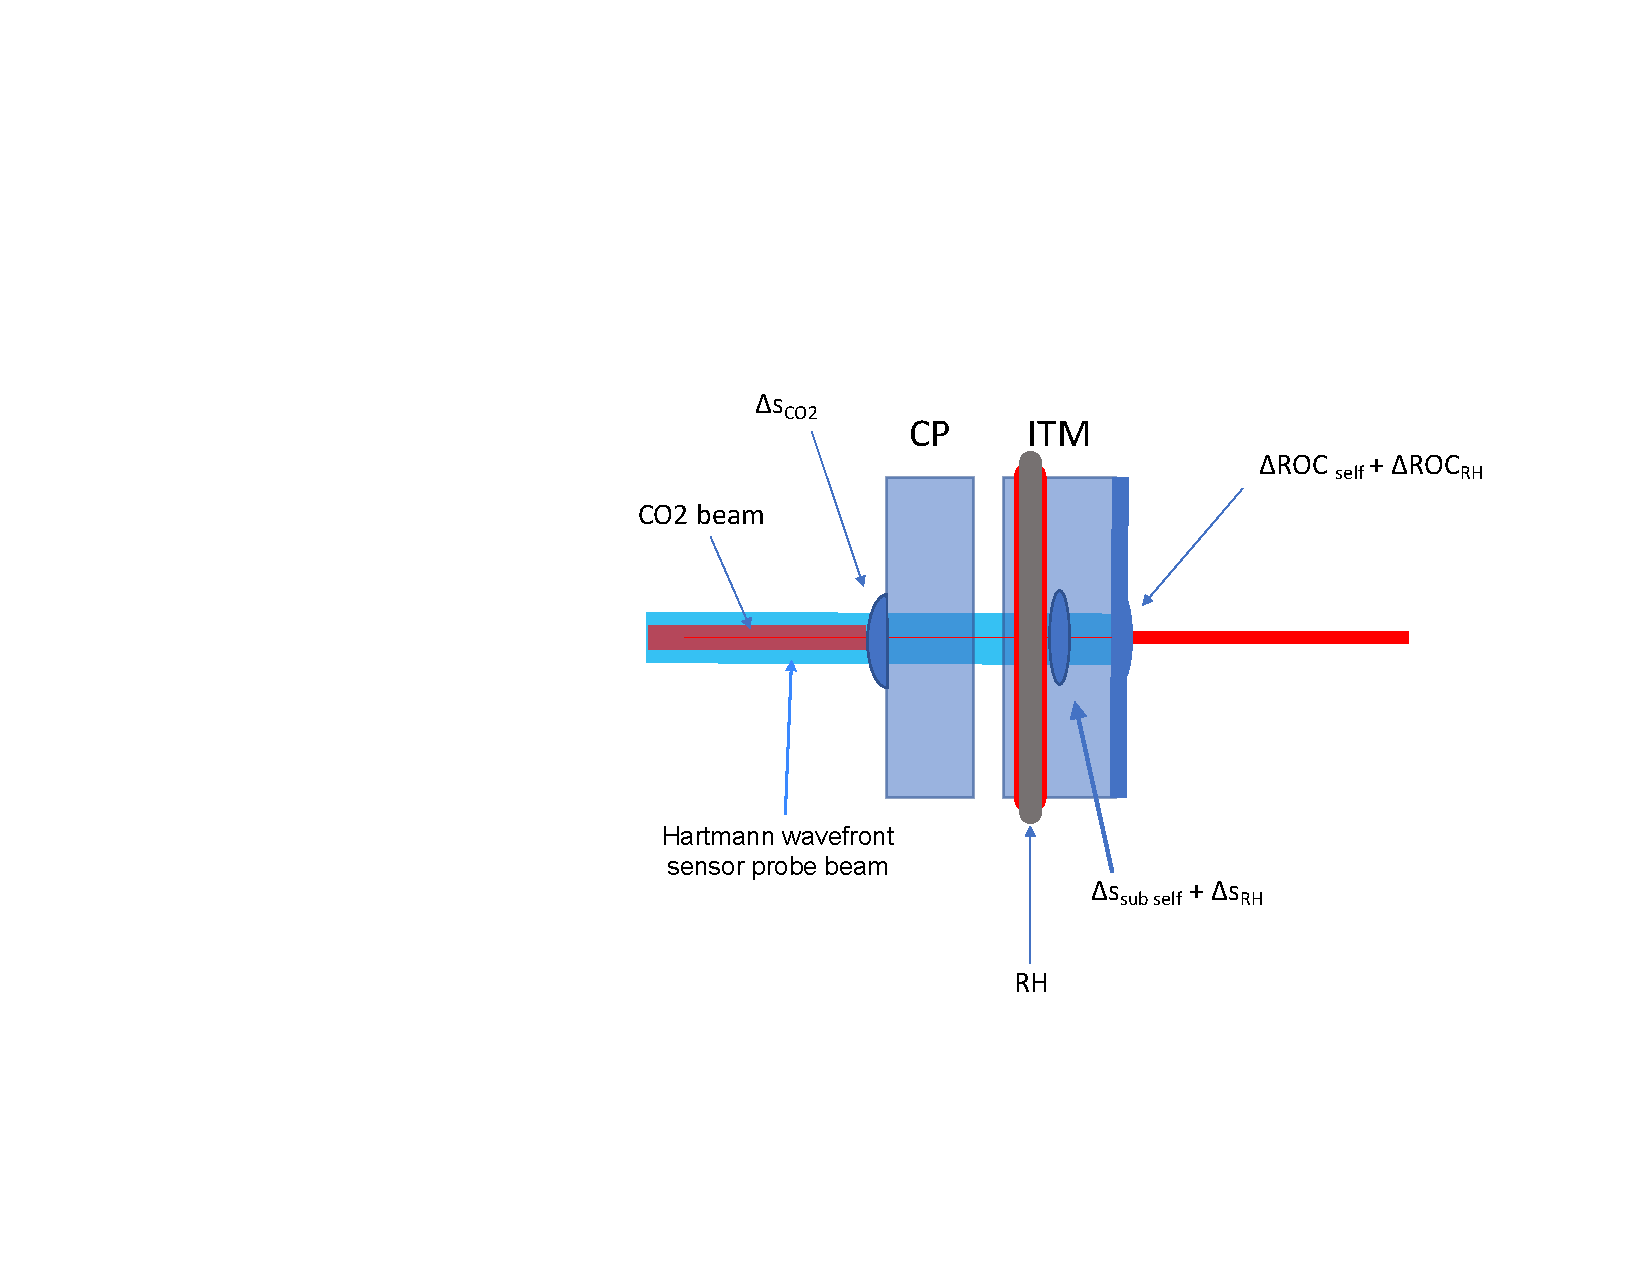
\includegraphics[width=\textwidth]{TCS/FP_input_coupler.pdf}
%	\caption{Thermal compensation at a single Fabry-P\'{e}rot input mirror coupler for ALIGO.}
%	\label{fig:meas}
%\end{figure}

\begin{figure}[H]
	\begin{subcaptiongroup}
		\centering
		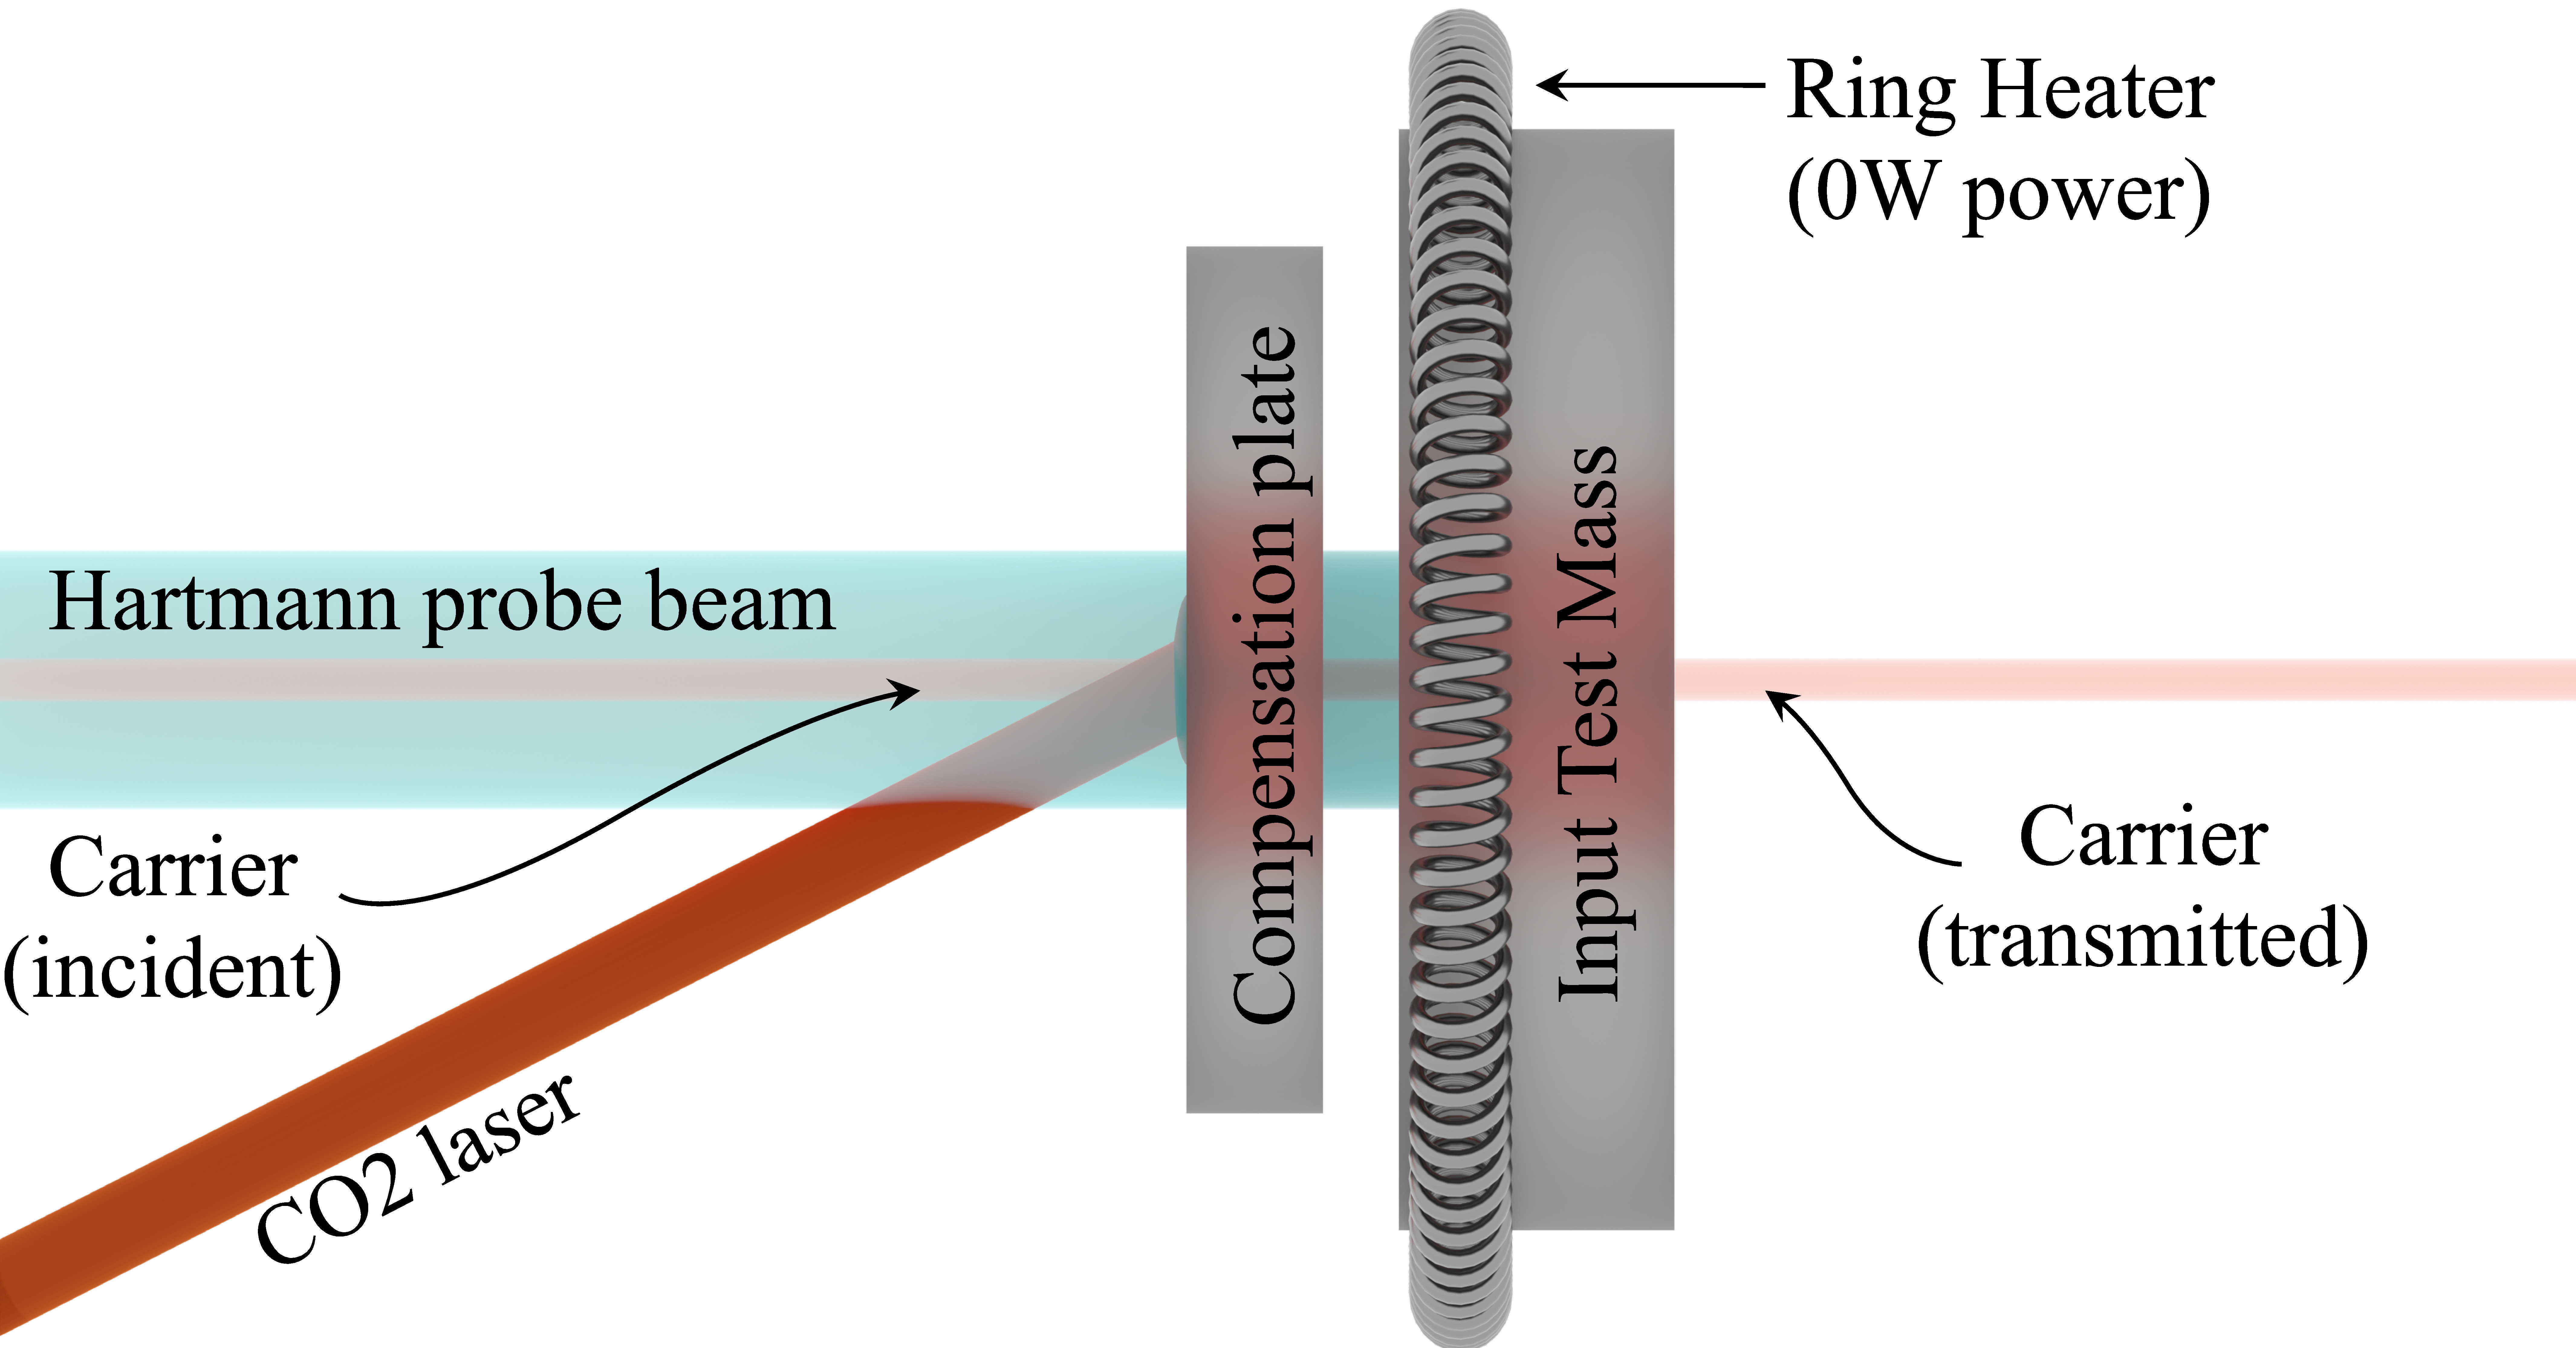
\includegraphics[width=.6\textwidth]{TCS/ITMYarminp/annotated/max/ITMYinp_lowcirc.pdf}
		\caption{CO2 actuator set to replicate projected carrier thermo-optic response, with an off resonance circulating beam.}\label{subfig:TCSinp_lowcirc}
%		\caption{(A) The incident carrier beam and (B) }\label{TCSinp_lowcirc}
		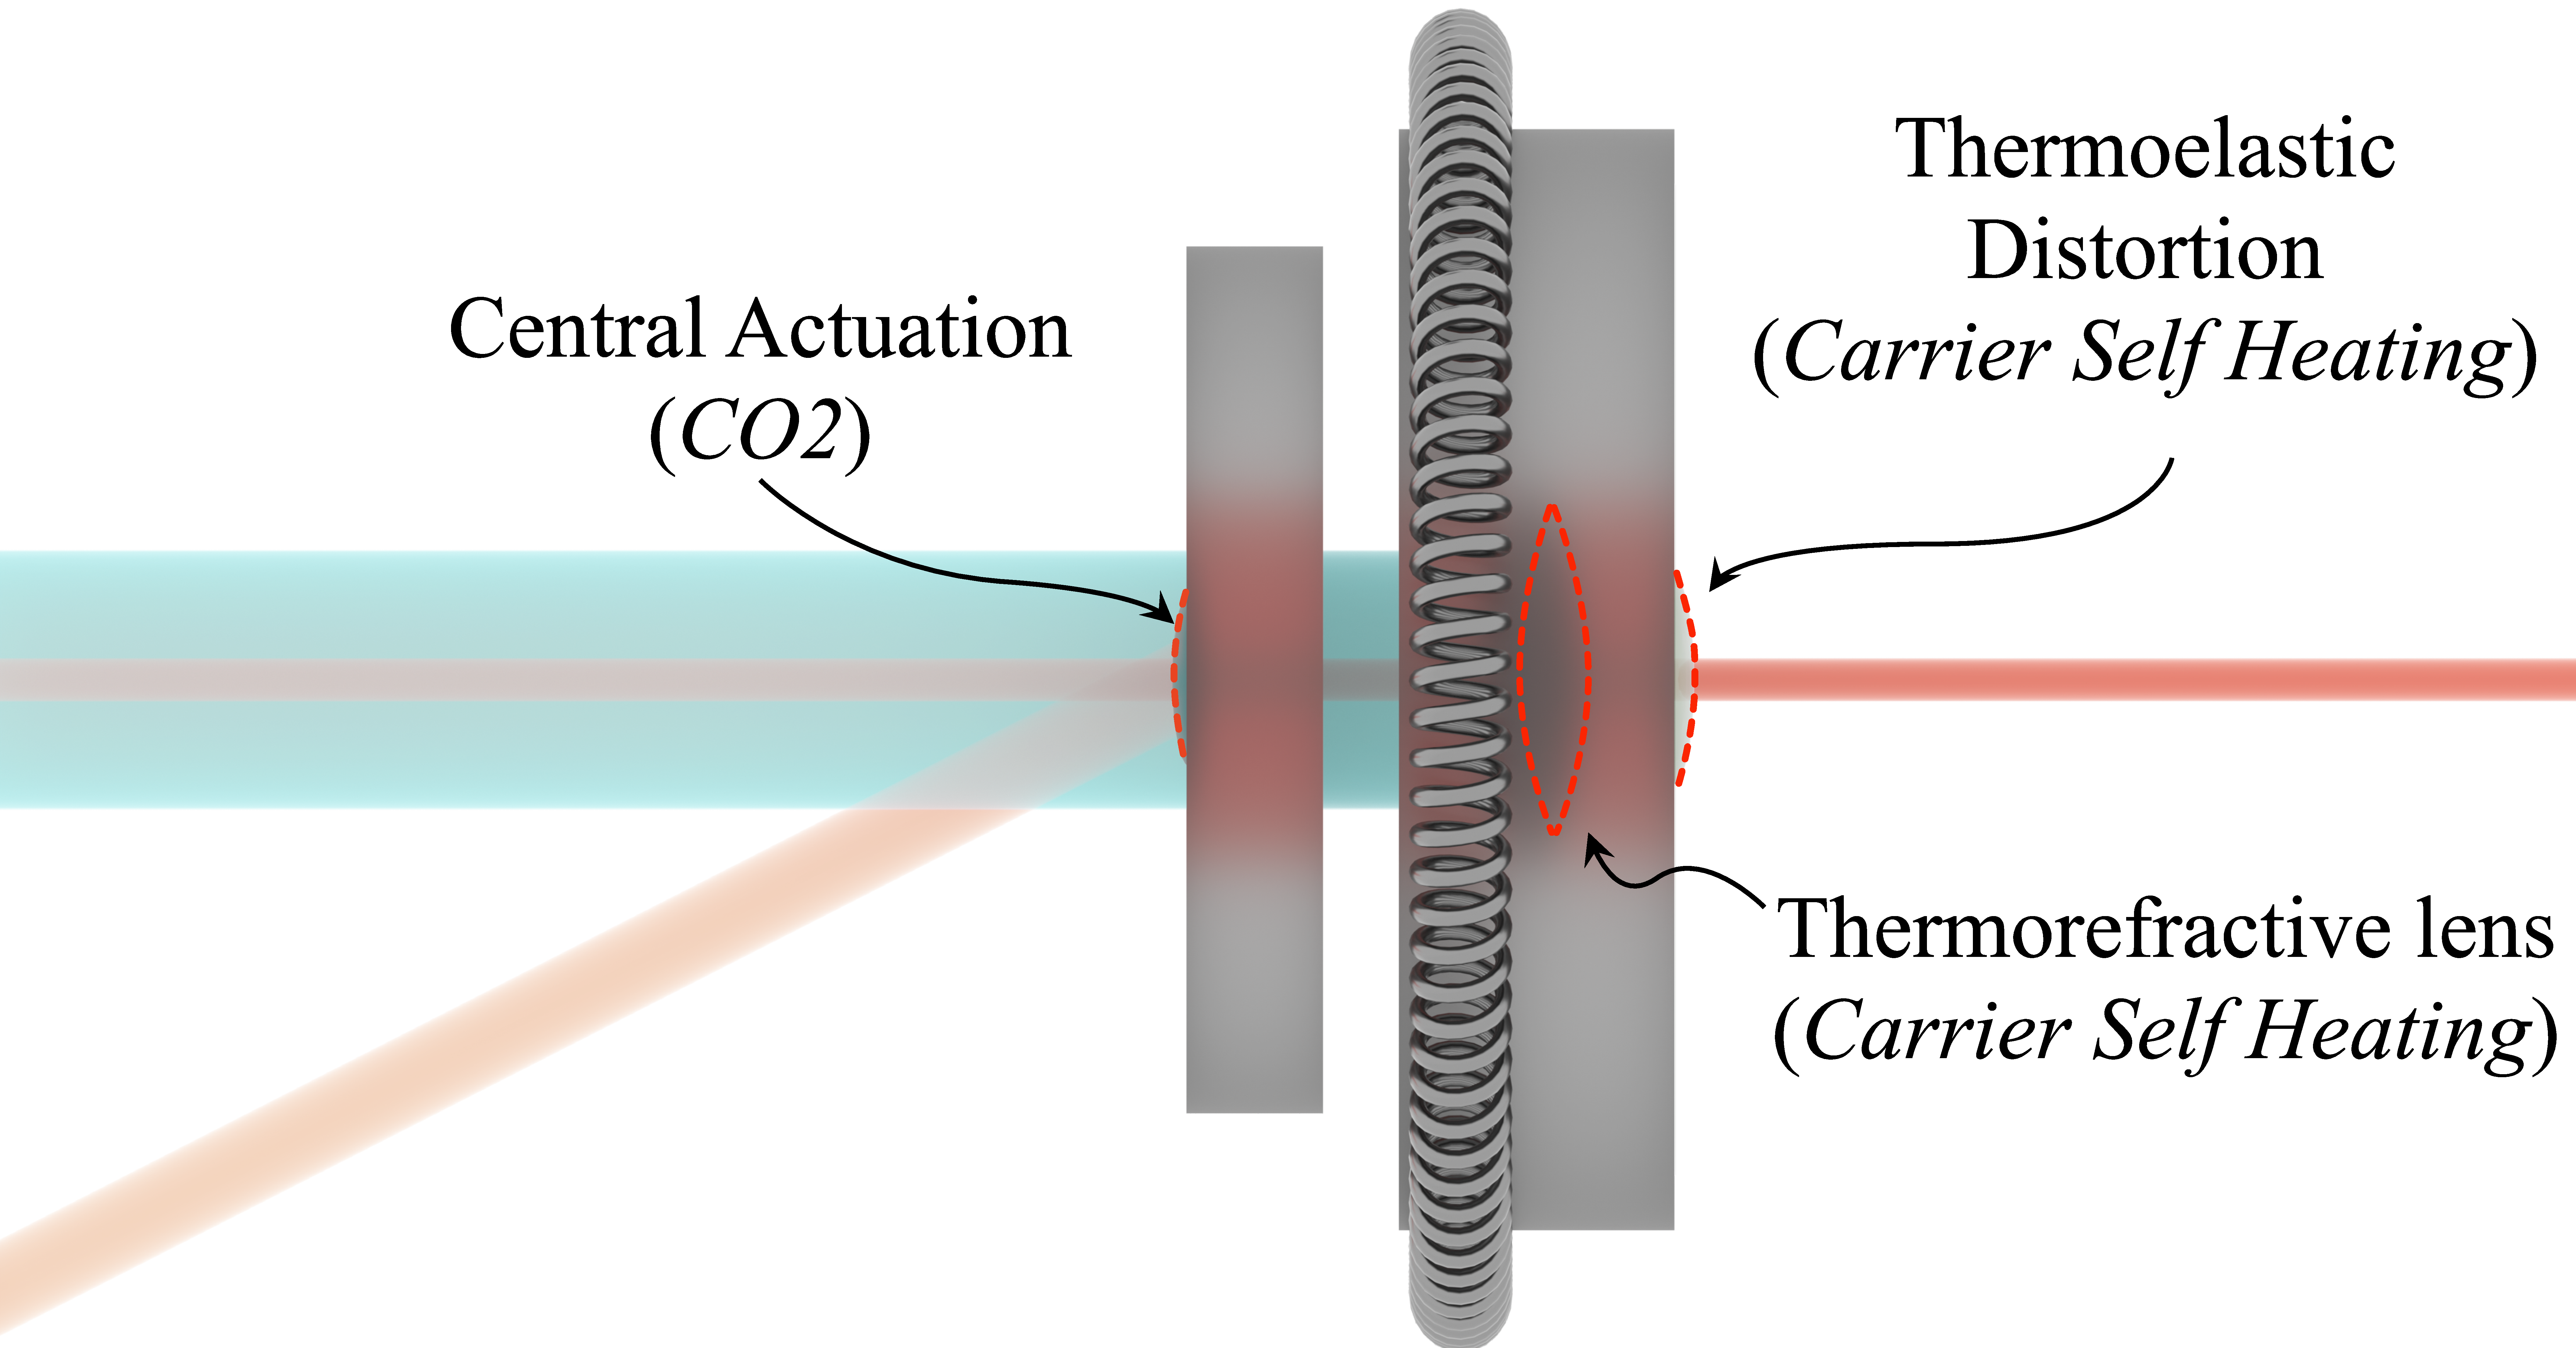
\includegraphics[width=.6\textwidth]{TCS/ITMYarminp/annotated/max/ITMYinp_intermcirc.pdf}
		\caption{Arm cavity resonance, with reduced CO2 central actuation power and increased arm cavity input power. The uniform thermo-optic distortion from the high power circulating carrier imposes a differential thermo-refractive lens and thermo-elastic HR surface change to the ITM, placing a low upper to the circulating power limit without annular ring heater actuation.}\label{subfig:TCSinp_intcirc}
%		\caption{Arm cavity resonance, with reduced CO2 central actuation power and increased arm cavity input power. The uniform thermo-optic distortion from the high power circulating carrier imposes a differential thermorefractive and thermoelastic HR surface change to the ITM, placing a low upper to the circulating power limit without annular ring heater actuation.}\label{TCSinp_intcirc}
		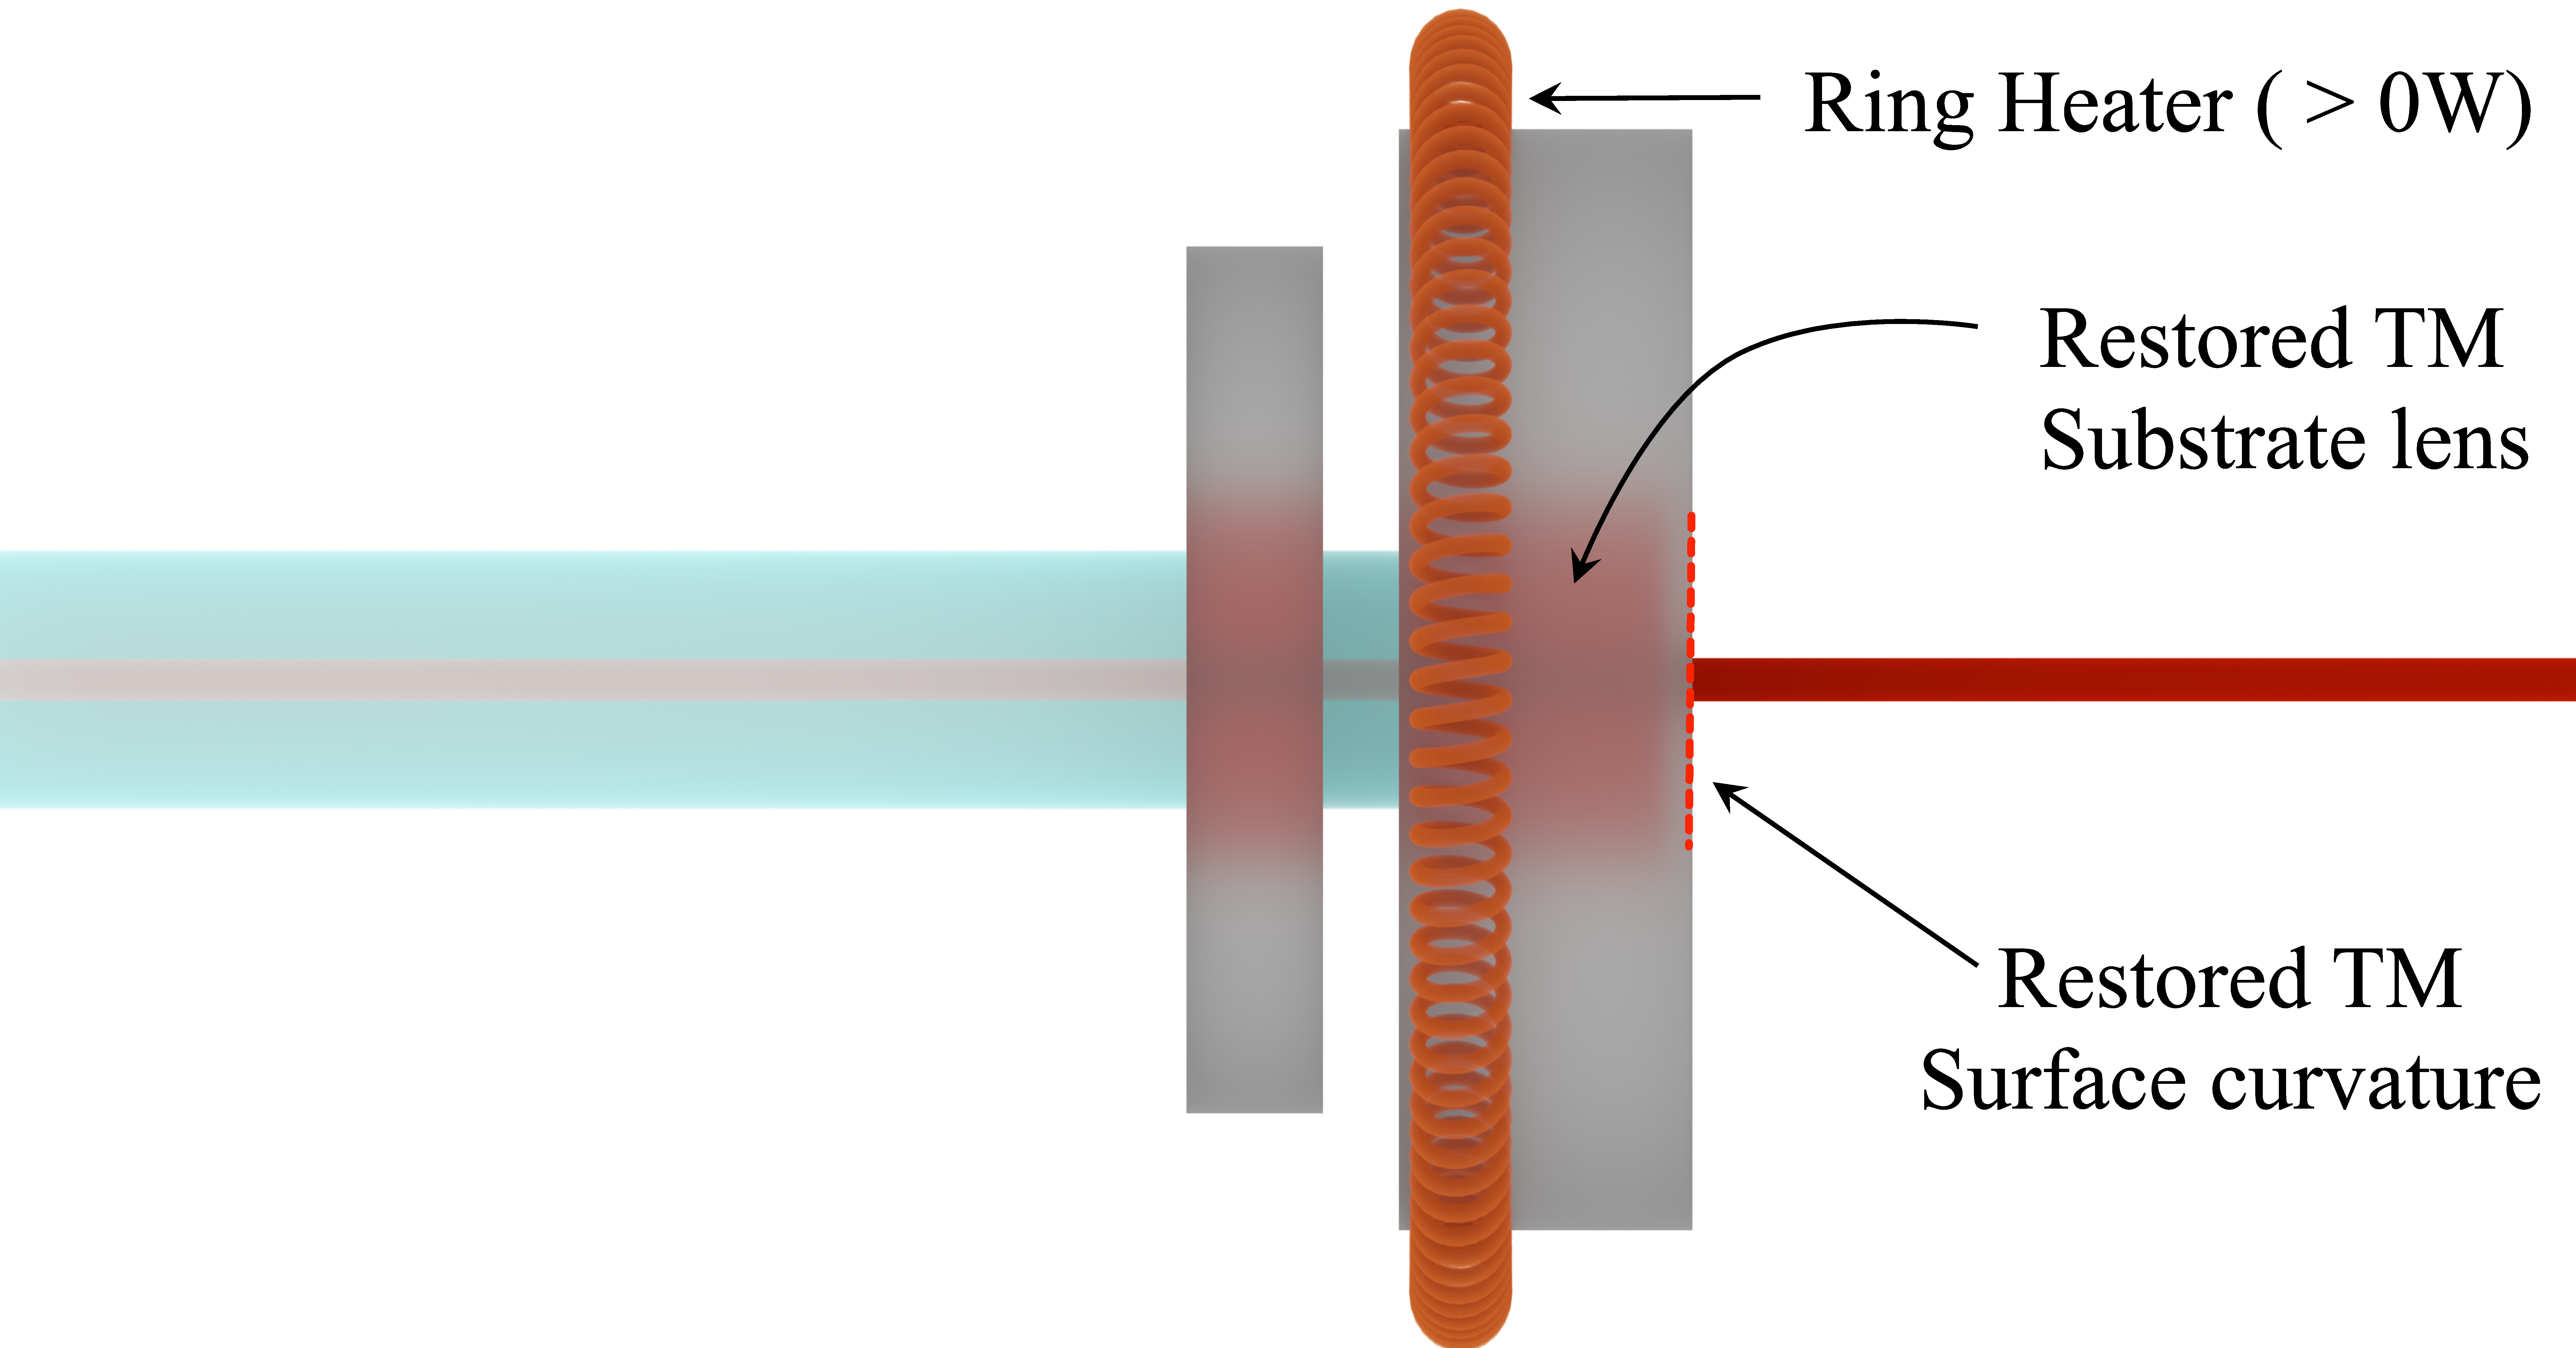
\includegraphics[width=.6\textwidth]{TCS/ITMYarminp/annotated/max/ITMYinp_highcirc.pdf}
		\caption{Maximum circulating arm power, with annular heating and no central CO2 actuation. The careful timing and calibration of the CO2 / RH actuators allow designed power / GW detector sensitivity to be reached.}\label{subfig:TCSinp_highcirc}
%		\caption{Maximum circulating arm power, with annular heating and no central CO2 actuation. The careful timing and calibration of the CO2 / RH actuators allow designed power / GW detector sensitivity to be reached.}\label{TCSinp_highcirc}
	\end{subcaptiongroup}
	\caption{ALIGO thermal compensation design at the input of a single Fabry-P\'{e}rot arm cavity. Though not the only location of thermal mode matching actuators, a careful look here can adequately demonstrates their capabilities and motivates their careful tuning while comissioning the current generation of gravitational wave detectors at high power.}
	\label{fig:meas}
\end{figure}


\section{Detector Noise}

\section{Coating Thermal Noise}
Contributions of categorized noises for gravitational wave detectors are organized in a ''noise budget", comprised of a collection of technical (noise imposed by the practical operation of the detector) and fundamental (inherent physical limitations of DRFPMIs by design) noise sources that impose limitations on gravitational wave detection.
%% Contributions of categorized noises for gravitational wave detectors the ''noise budget" ((LHO and LLO O3?) or just GWINC?)}

\subsection{Brownian Thermal Noise}
%% Might move this section back to the $\algaas$ Electro-optic noise chapter
In 1827 the Scottish botanist Robert Brown noticed a constant motion of pollen particulates on the surface of water; witnessing randomized collisions of the water molecules holding a kinetic energy proportional to the temperature ($k_BT$) \cite{Brown:1828}. It is because of his documented observations we name the phenomena Brownian motion. And although the observations were on motion of particulates in liquids, molecules and atoms within gases and solids also exhibit Brownian motion. For high precision optical experiments operating at room temperature (and higher due to high power resonant beams), understanding how much differential phase noise is imparted on the interferometer light passing through and reflecting from core optics is crucial. This requires knowledge of the mean squared displacement from each degree of freedom of the system which can be realized through the Fluctuation Dissapation theorem. Derived by H.B. Callen and T.A. Welton, the theorem states that for a randomly fluctuating linear force \cite{Callen:1951}:

%% Further insight into Brownian motion was explored by Einstein where he was able to relate the mean-square displacement of a particle of radius $r_\mathrm{sph}$ on a fluid with viscosity $\eta$.
 %%\begin{equation}
 %%\overline{x^2} = k_B T  \frac{1}{3 \pi \eta  r_\mathrm{sph}}
 %%\end{equation}
 %%This relation has important implications about how the random motion or fluctuations of a particulate (the pollen) is influenced (dissipated) by the viscosity of the surrounding medium (water).

\begin{equation}
F_x^2(f) = 4 k_B T\; \Re[Z]
\end{equation}

 \noindent Where $\Re[Z]$ is the real part of the impedance of the system. This impedance directly relates to equations of motion:

 \begin{equation}
 Z = \frac{F}{\dot{x}}
 \end{equation}

\noindent Another useful form is the power spectrum of the fluctuating motion:
\begin{equation}\label{fdtpsd}
x^2 (f)  = \frac{4k_B T}{(2 \pi f)^2}\; \Re[Y]
\end{equation}

Where $Y$ is the inverse of the impedance or admittance. With this power spectra, modelling and budgeting notable LIGO fundamental noise contributions attributed to the choice of the materials used for mirror substrates, and highly reflective mirror coatings becomes less daunting. Though adequate modelling of internal force couplings for the aforementioned components is required.

\subsubsection{Internal friction in Materials and Loss angle}

Zener provides a model of the internal friction of materials incorporating anelasticity into the equations of motion \cite{zener:1948}:

\begin{equation}
F = k(1+i\phi)x + m\ddot{x}
\end{equation}


Where $m$ is mass attached to a spring with a spring constant $k(1+ i\phi)$ incorporating the degree of anelasticity $\phi$. From equations 3.5 and 3.3 we perform a Laplace transform and acquire the following form of admittance:
\begin{equation}
Y(s) = \frac{\dot{x}(s)}{F(s)} = \frac{-s}{k(1+i\phi) + ms^2}
\end{equation}

\noindent Or more transparently the Fourier representation since we assume a linear time invariant system:

\begin{equation}\label{admitint}
Y(\omega) = \frac{\dot{x}(\omega)}{F(\omega)} = \frac{-i\omega}{k(1+i\phi) - m\omega^2} = \frac{k \omega \phi - i \omega (k - m \omega^2)}{(k-m\omega^2)^2 +k^2 \phi^2}
\end{equation}

\noindent Plugging equation \ref{admitint} back into \ref{fdtpsd}:

\begin{equation}
x^2 (f)  = \frac{2k_B T}{\pi}\frac{k\phi}{(k-4\pi^2 m f^2)^2 + k^2 \phi^2}
\end{equation}
Computing the admittance from a Gaussian beam impinging upon a HR mirror can require expansion of all individual mechanical degrees of freedom of the test mass system across a relevant frequency range, and with that approach convergence is not guaranteed. Saulson and Gonzalez provide an alternative method to computing the admittance coined the ``direct approach" by Levin when computing the noise from a Gaussian beam on a LIGO HR test mass. The admittance can be acquired through:

\begin{equation}\label{admitdirec}
\Re[Y] = \frac{W_\mathrm{diss}}{F_o^2}
\end{equation}

\noindent $W_\mathrm{diss}$ is the dissipated power from the system due to an oscillating force $F_o$. This form of the admittance reveals an important result of the fluctuation dissapation theorem where an undriven system with a dissapative actor, imparts motion to the degrees of freedom via a driving force by virtue of that same actor at finite temperatures. This direct approach also allows the surface pressure applied by the Gaussian beam to interrogate which mechanical modes of the test mass impose a significant energy when \ref{admitdirec} is plugged into \ref{fdtpsd}. In the case of the gaussian beam / uncoated test mass studied by Levin \cite{levin:1998}:

\begin{equation}
S_x(f) = \frac{4 k_B T}{f} \frac{1-\sigma^2}{\pi^3 E_o r_o} I\phi \bigg[1- O\bigg( \frac{r_o}{R} \bigg)\bigg]
\end{equation}

%this requires that the driving force used in a lab mimics that of a force from a centered Gaussian beam.

%%Refer to Levin appendix for more on how elasticity parameters are introduced?
Where $\phi$ and $E_o$ are the Poisson ratio and Young's modulus respectively, and $O(\frac{r_o}{R})$ contains a correction term contribution as a function of the small beam radius ($r_o$) relative to the mirror radius ($R$).

\subsubsection{Coating Brownian thermal noise}
Further investigations into the beam/optic system utilizing this approach and elasticity theory led to a deeper understanding about Brownian thermal noise contributions from LIGO test masses (substrate, suspensions, HR coating). Levin mentions, with details from Harry, that the noise contributed by a lossy mirror coating is proven to be to be the most significant contributor of brownian thermal noise. Hong provides a power spectral density \cite{Hong:2013}:

\begin{equation}
S_j^X = \frac{4k_B T \lambda \phi_x^j(1- \sigma_j - 2 \sigma_j^2)}{3 \pi^2 f Y_j (1-\sigma_j)^2 \omega_o^2}
\end{equation}

Where X represents bulk and shear with j = odd (material 1) and j = even (material 2) alternating layers representing high and low index materials j = odd (material 1) j = even (material 2) for an HR coating.

\begin{figure}[H]
    \begin{center}
    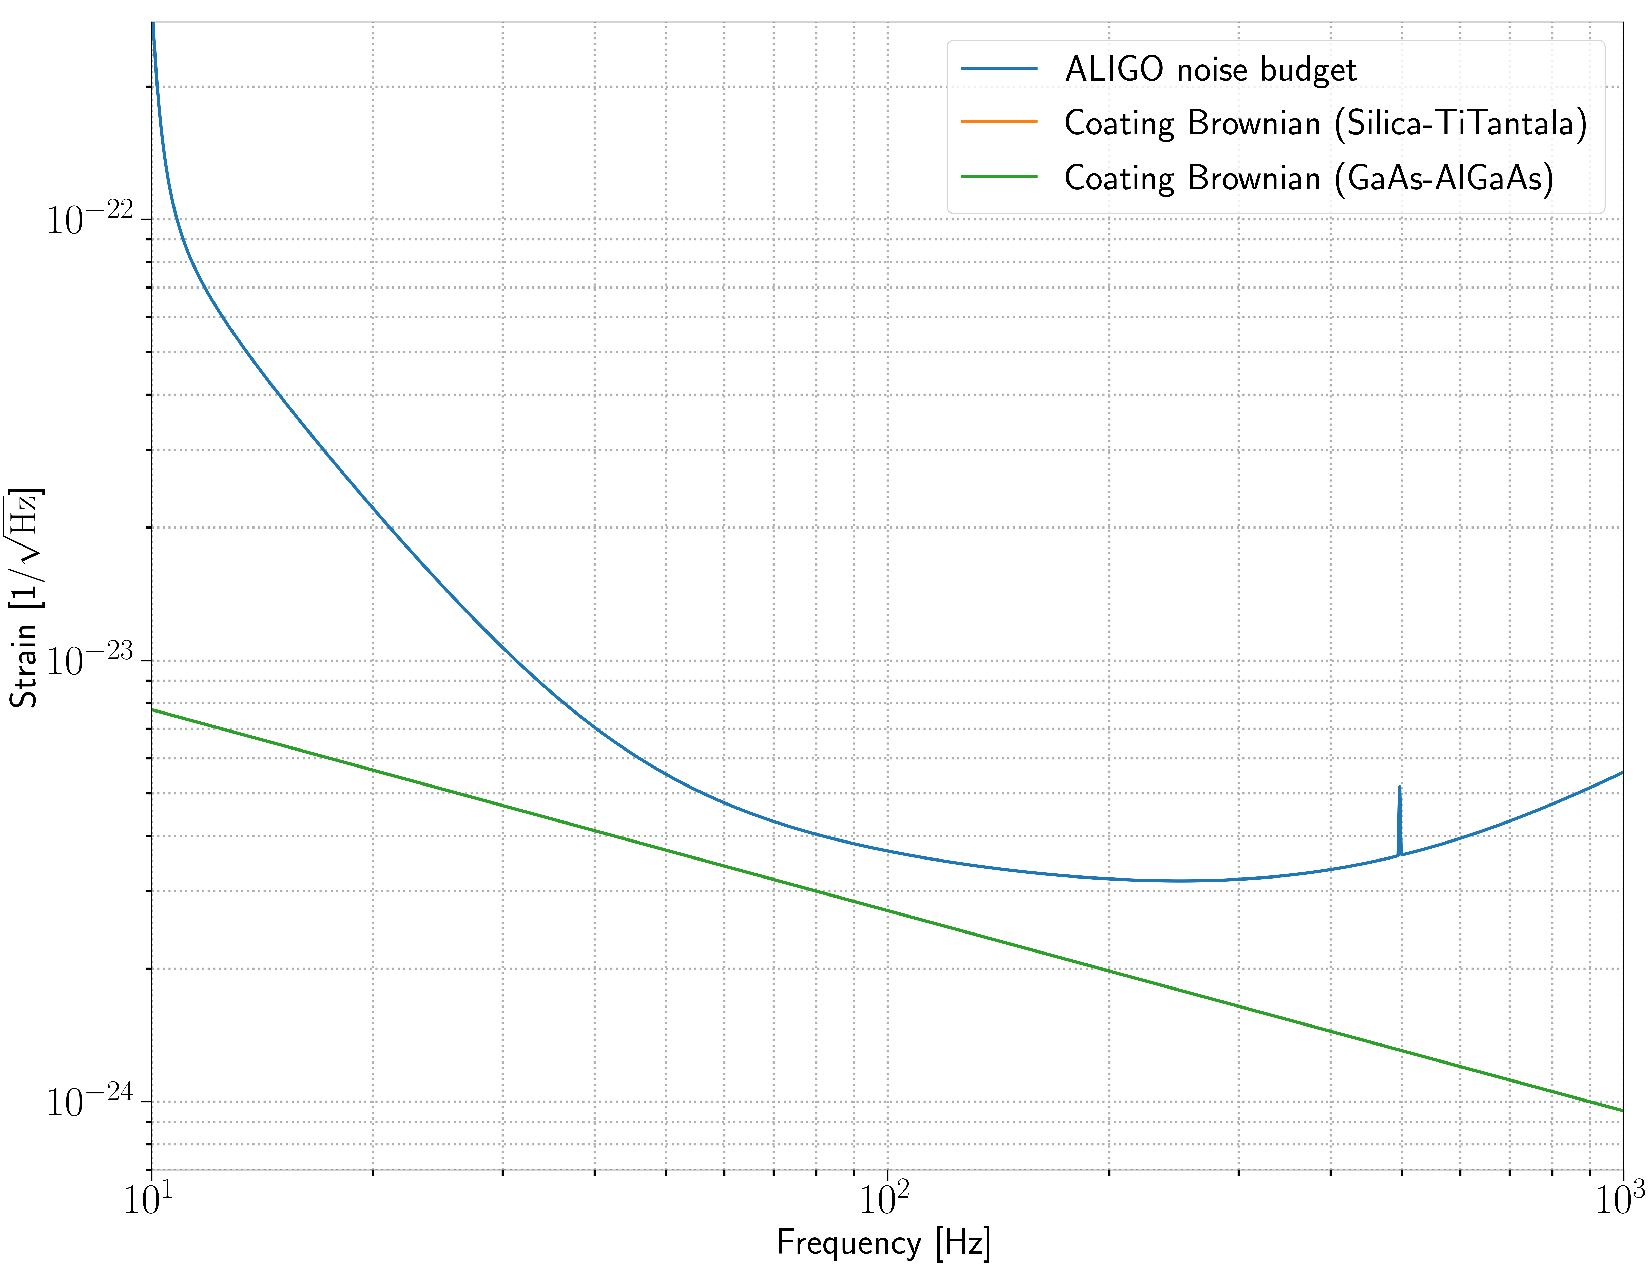
\includegraphics[width=.9\textwidth]{ALGAAS/aligo_nb_plus_cbn.pdf}
    \end{center}
    \caption{ALIGO noise budget placeholder for silica-tantala, and gaas-algaas brownian noise comparison}
\label{fig:aligo_tn_comparison}
\end{figure}

\subsubsection{$\mathrm{SiO_2}/\mathrm{TiO_2:Ta_2O_5}$ coating parameters}
Currently the LIGO interferometers deposit $\lambda$/4 stacks of silica and titania doped tantala on fused silica test mass substrates. Effective loss angle measurements \cite{Harry:06}

\textbf{Current $\mathrm{SiO_2}/\mathrm{TiO_2:Ta_2O_5}$ elasticity params, power spectra, and strain spectral density (order of magnitude estimate)}

\subsubsection{$\gaas$/$\algaas$ coating parameters}
%%Specific coating parameters for most promising $\algaas$ candidates? Chat with Steve. Or just mention parameters that are listed in Cole 2013
\cite{Cole:2013}

%% Insert computed curves of the most precise and recent (effective) loss angle measurements (Nick Demos measurements?). More instructive to plot strain spectral density or displacement power spectra

\noindent Currently thermal noise from the $\mathrm{SiO_2}/\mathrm{TiO_2:Ta_2O_5}$ optical coatings is the largest contributor of Brownian noise in LIGO compared to estimated substrate and suspension thermal noise \cite{Harry:06}. As of the end of O3, Brownian thermal noise is estimated to be ? orders of magnitude below the current sensitivity and it will prove to be the limiting source of noise as that sensitivity is increased with various other upgrades mitigating fundamental and technical noise. 
%% Already mentioned in intro prior to this thermal noise section. Need to re-iterate in more detail?

\newpage

\chapter{TCS comissioning for O3}
%% Hanford investigations

%% TCS schematic for LIGO Hanford for O3
%% TCS pre-loading
 %% Current methodology for tuning TCS
  %% Detail Hanford's methods
 %% Increasing RH tuning speed


%As shown in Chapter 1,  

\section{Motivation}
As seen in ~\autoref{sec:detcon}, increasing detector input power leads to a direct sensitivity increase to gravitational waves. And even using optics with ultra-low absorption ($\approx 400 \; \mathrm{ppb} \pm 150 \; \mathrm{ppb}$ \textcolor{red}{alog ? or point absorber paper}) there still are induced thermo-optic effects with a designed circulating arm power of 750 kW in the Fabry-P\'{e}rot cavity arms. Predicted thermal aberrations produced are a substrate lens with a relatively smaller lensing from the differential HR surface curvature. This time varying optical path length change integrated over the carrier phasefront produces mode mismatch and accumulates optical loss throughought GWDs and reduces sensitivity two-fold: loss of readout power, and reduced efficacy to produce squeezed light states in lowering the detector quantum noise limit.
\\
During O3a the LIGO Hanford observatory increased circulating arm power beyond 180 kW; emphasizing importance on properly tuned thermal compensation in O3 to avert arm-cavity/carrier-beam mode mismatch. Detailed in this chapter is a summary of related comissioning efforts at LHO to maintain interferometer mode matching including but not exclusive to: a primer on the ALIGO adaptive optics schema (TCS), citations on the initial computed O3 TCS pre-load, the development and implementation of real-time digital filtering for an improved ring heater actuation response by a factor of $\approx 6$, and the impacts of high absorption points aka point absorbers discovered on arm cavity test masses along with the some efforts to mitigate them.

\subsection{Thermal Compensation System}
The thermal compensation system (TCS) is comprised of an adaptive optics system that uses four Hartmann wavefront sensors (HWS) combined with actuators of two varieties: annular ring heaters and CO2 lasers. The system is meant to address the problem of dynamic mode matching conditions throughout the interferometer as high power operation is inevitable towards reaching ALIGO design sensitivity. Select core optics (Fabry-Perot cavity mirrors) are strategically monitored for differential lensing. 

\subsubsection{Actuation}
Both ITMs and ETMs utilize mode matching actuation, though they are not prescribed equal treatment; all Fabry-P\'{e}rot cavity mirrors possess negative lens actuation in the form of a wound nichrome wire annulus that outlines the outer barrel of the test masses while CO2 actuation is applied to a compensation plate (CP) \footnote{intended to decouple CO2 laser noise from the highly sensitive FP test mass} located between the beam splitter (BS) and the input test mass (ITM) to counter or replicate the substrate lens via negative or positive actuation respectively~\cite{brooks:aigwd2019}.

\subsubsection{Sensing Optical Path Distortion}
Quantifying thermal distortion from both carrier as well as thermal actuators is performed with a set of four Hartmann wavefront sensors; each one measuring the differential optical path distortion at each FP cavity test masses. The sensor probe beams \footnote{differing wavelengths of 800 nm and 833 nm for the X and Y arms to mitigate crosstalk between sensing chains} make a double pass through the test mass mirror substrate for all arm cavity mirrors and map the HR mirror surface; while making an additional double pass through a compensation plate (CP) installed between the BS and the ITM for sensors at the interferometer vertex~\cite{aasi:2015}.

\begin{figure}[H]
	\begin{subcaptiongroup}
		\centering
		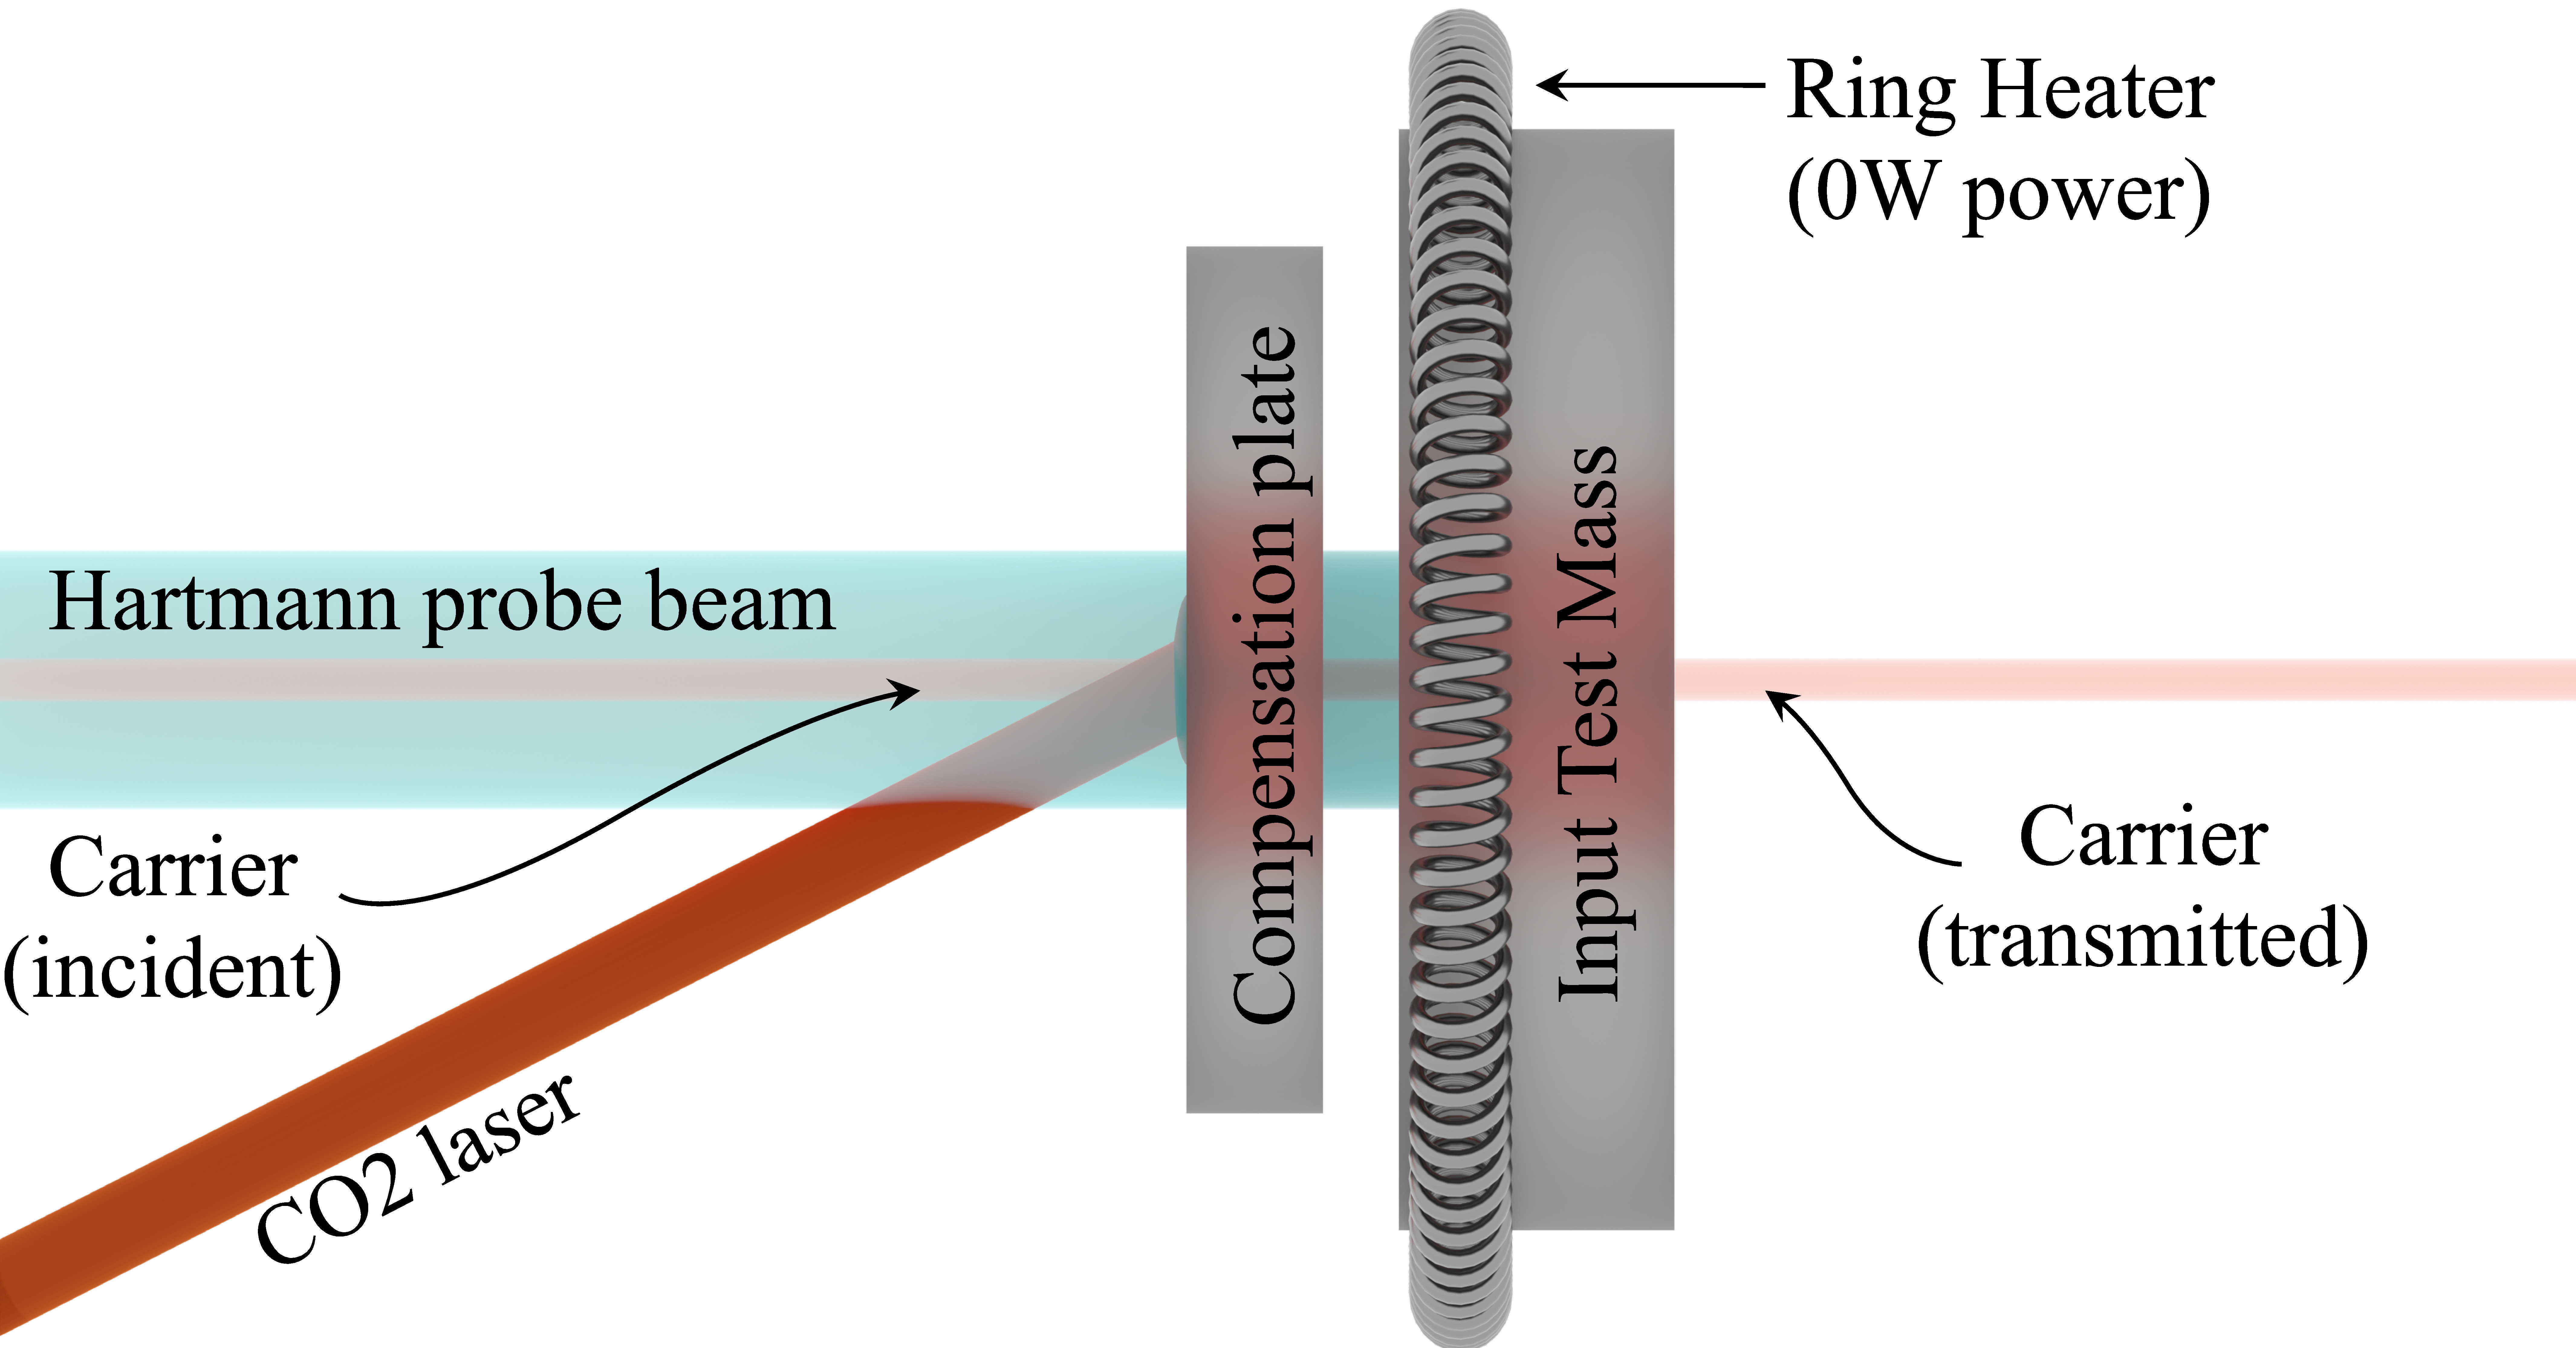
\includegraphics[width=.6\textwidth]{TCS/ITMYarminp/annotated/max/ITMYinp_lowcirc.pdf}
		\caption{CO2 actuator set to replicate projected carrier thermo-optic response, with an off resonance circulating beam.}\label{subfig:TCSinp_lowcirc}
%		\caption{(A) The incident carrier beam and (B) }\label{TCSinp_lowcirc}
		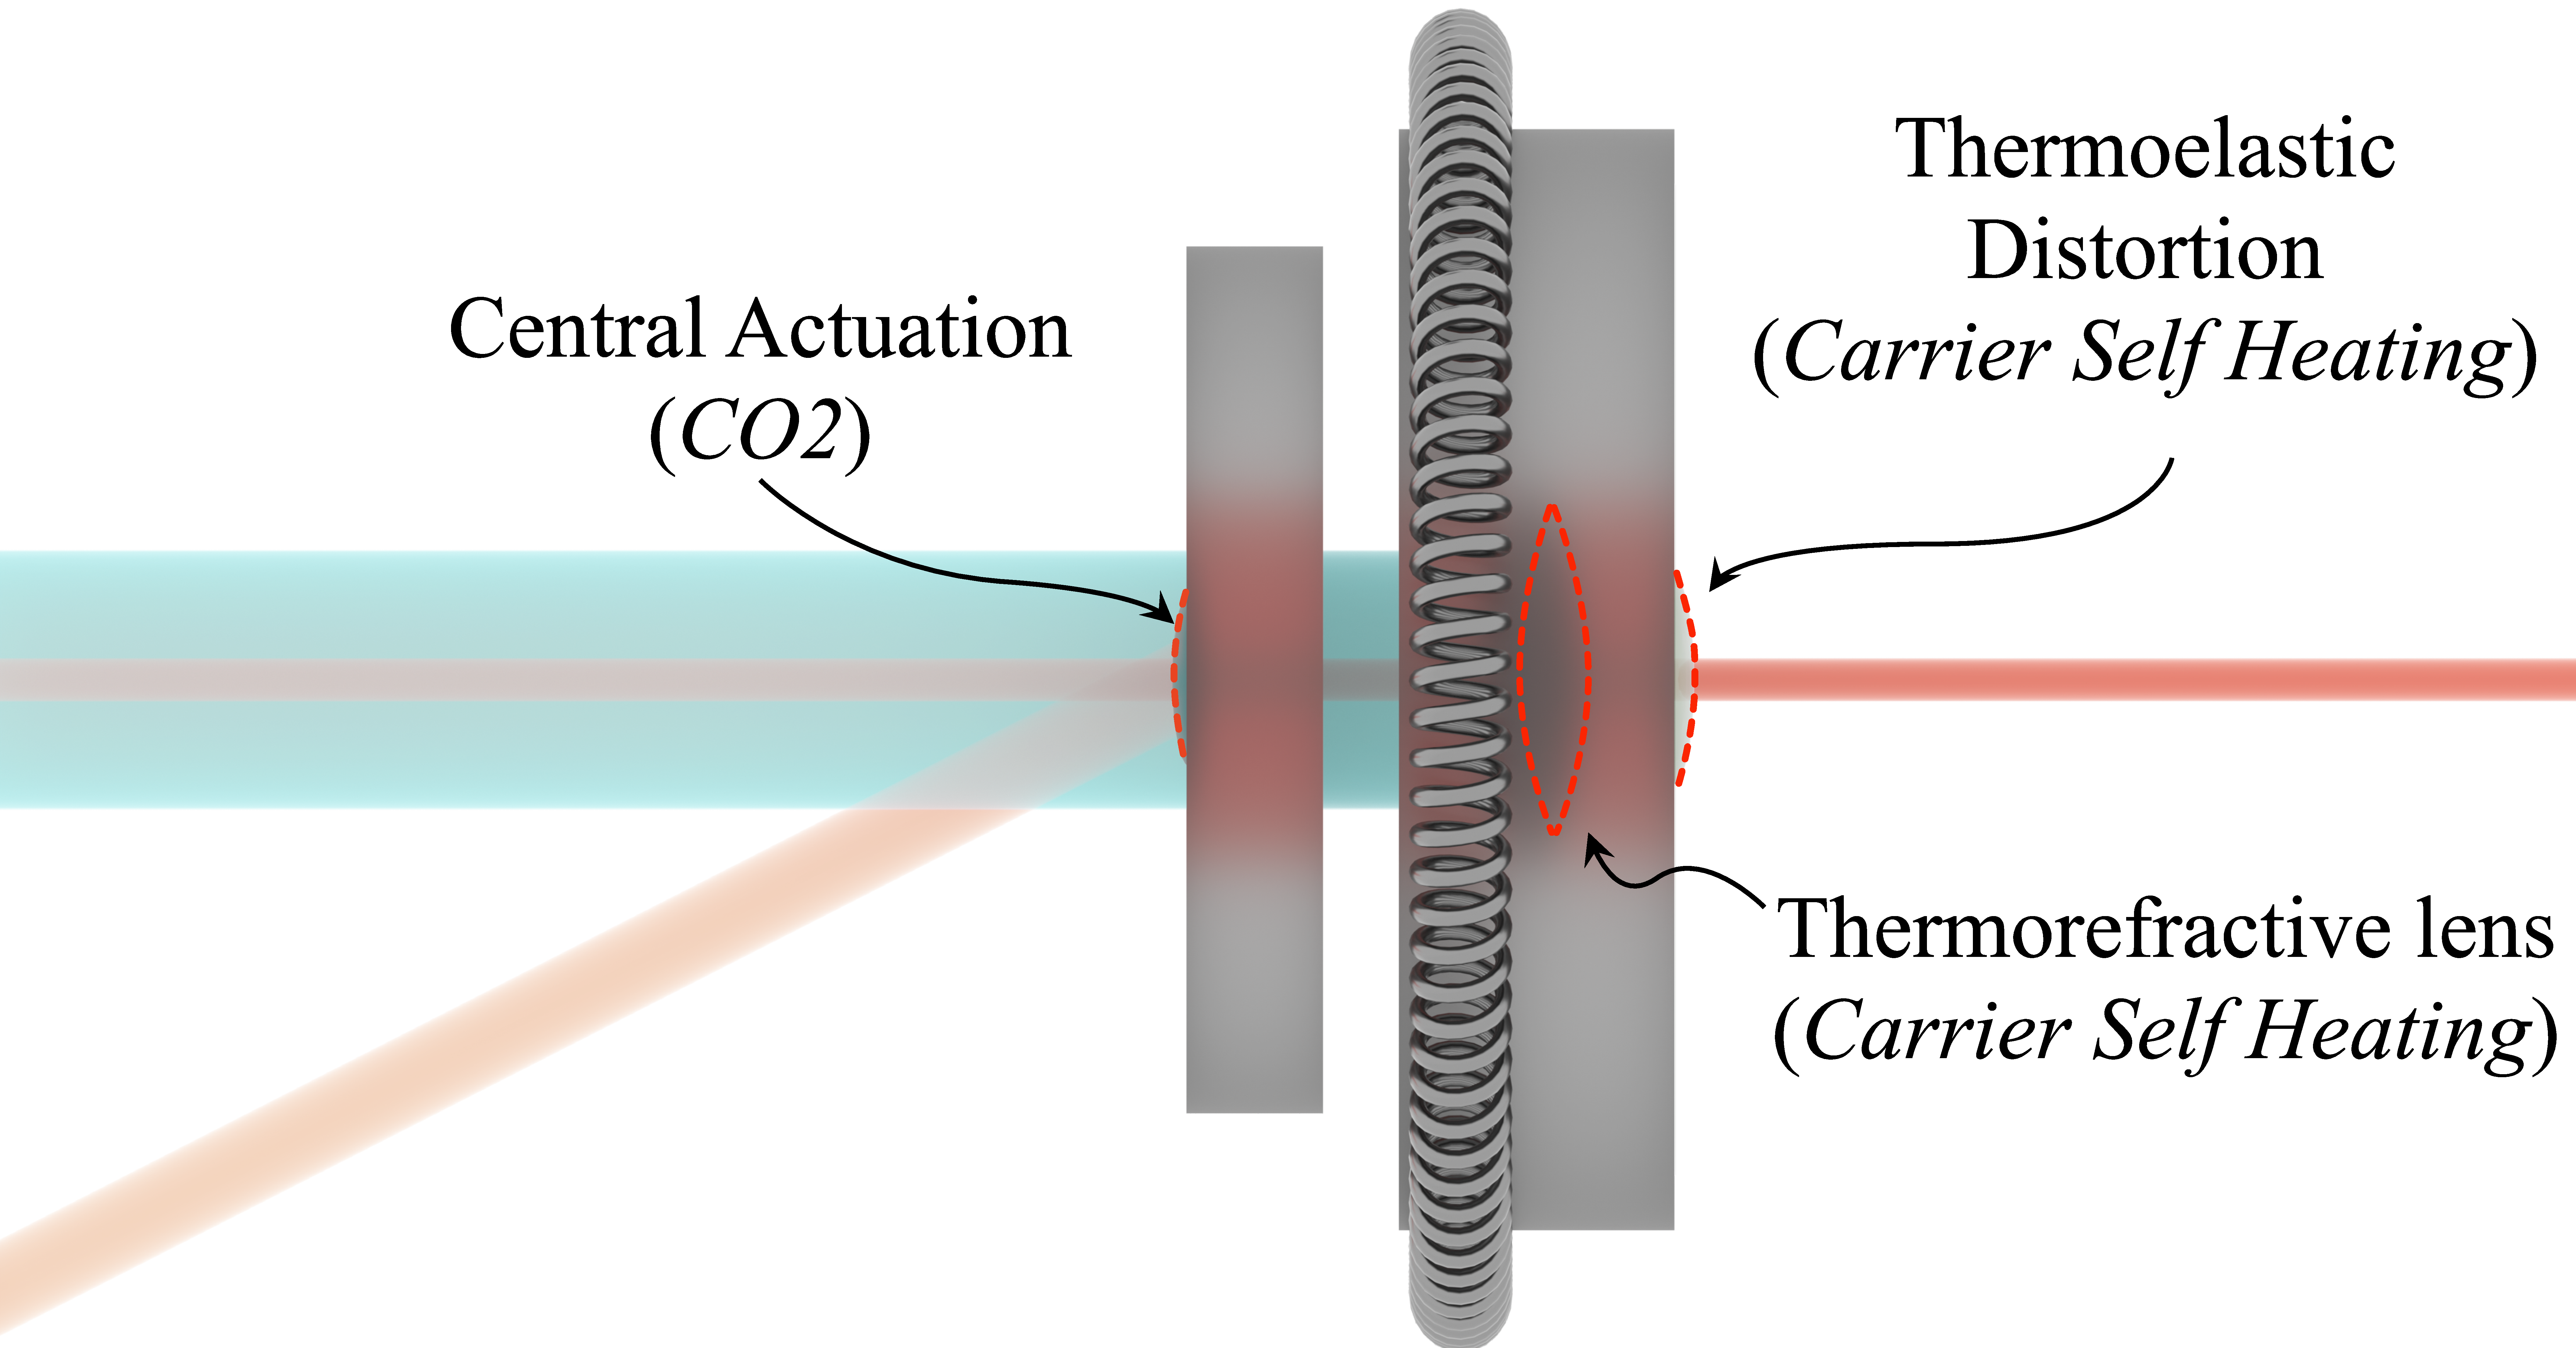
\includegraphics[width=.6\textwidth]{TCS/ITMYarminp/annotated/max/ITMYinp_intermcirc.pdf}
		\caption{Arm cavity resonance, with reduced CO2 central actuation power and increased arm cavity input power. The uniform thermo-optic distortion from the high power circulating carrier imposes a differential thermo-refractive lens and thermo-elastic HR surface change to the ITM, placing a low upper to the circulating power limit without annular ring heater actuation.}\label{subfig:TCSinp_intcirc}
%		\caption{Arm cavity resonance, with reduced CO2 central actuation power and increased arm cavity input power. The uniform thermo-optic distortion from the high power circulating carrier imposes a differential thermorefractive and thermoelastic HR surface change to the ITM, placing a low upper to the circulating power limit without annular ring heater actuation.}\label{TCSinp_intcirc}
		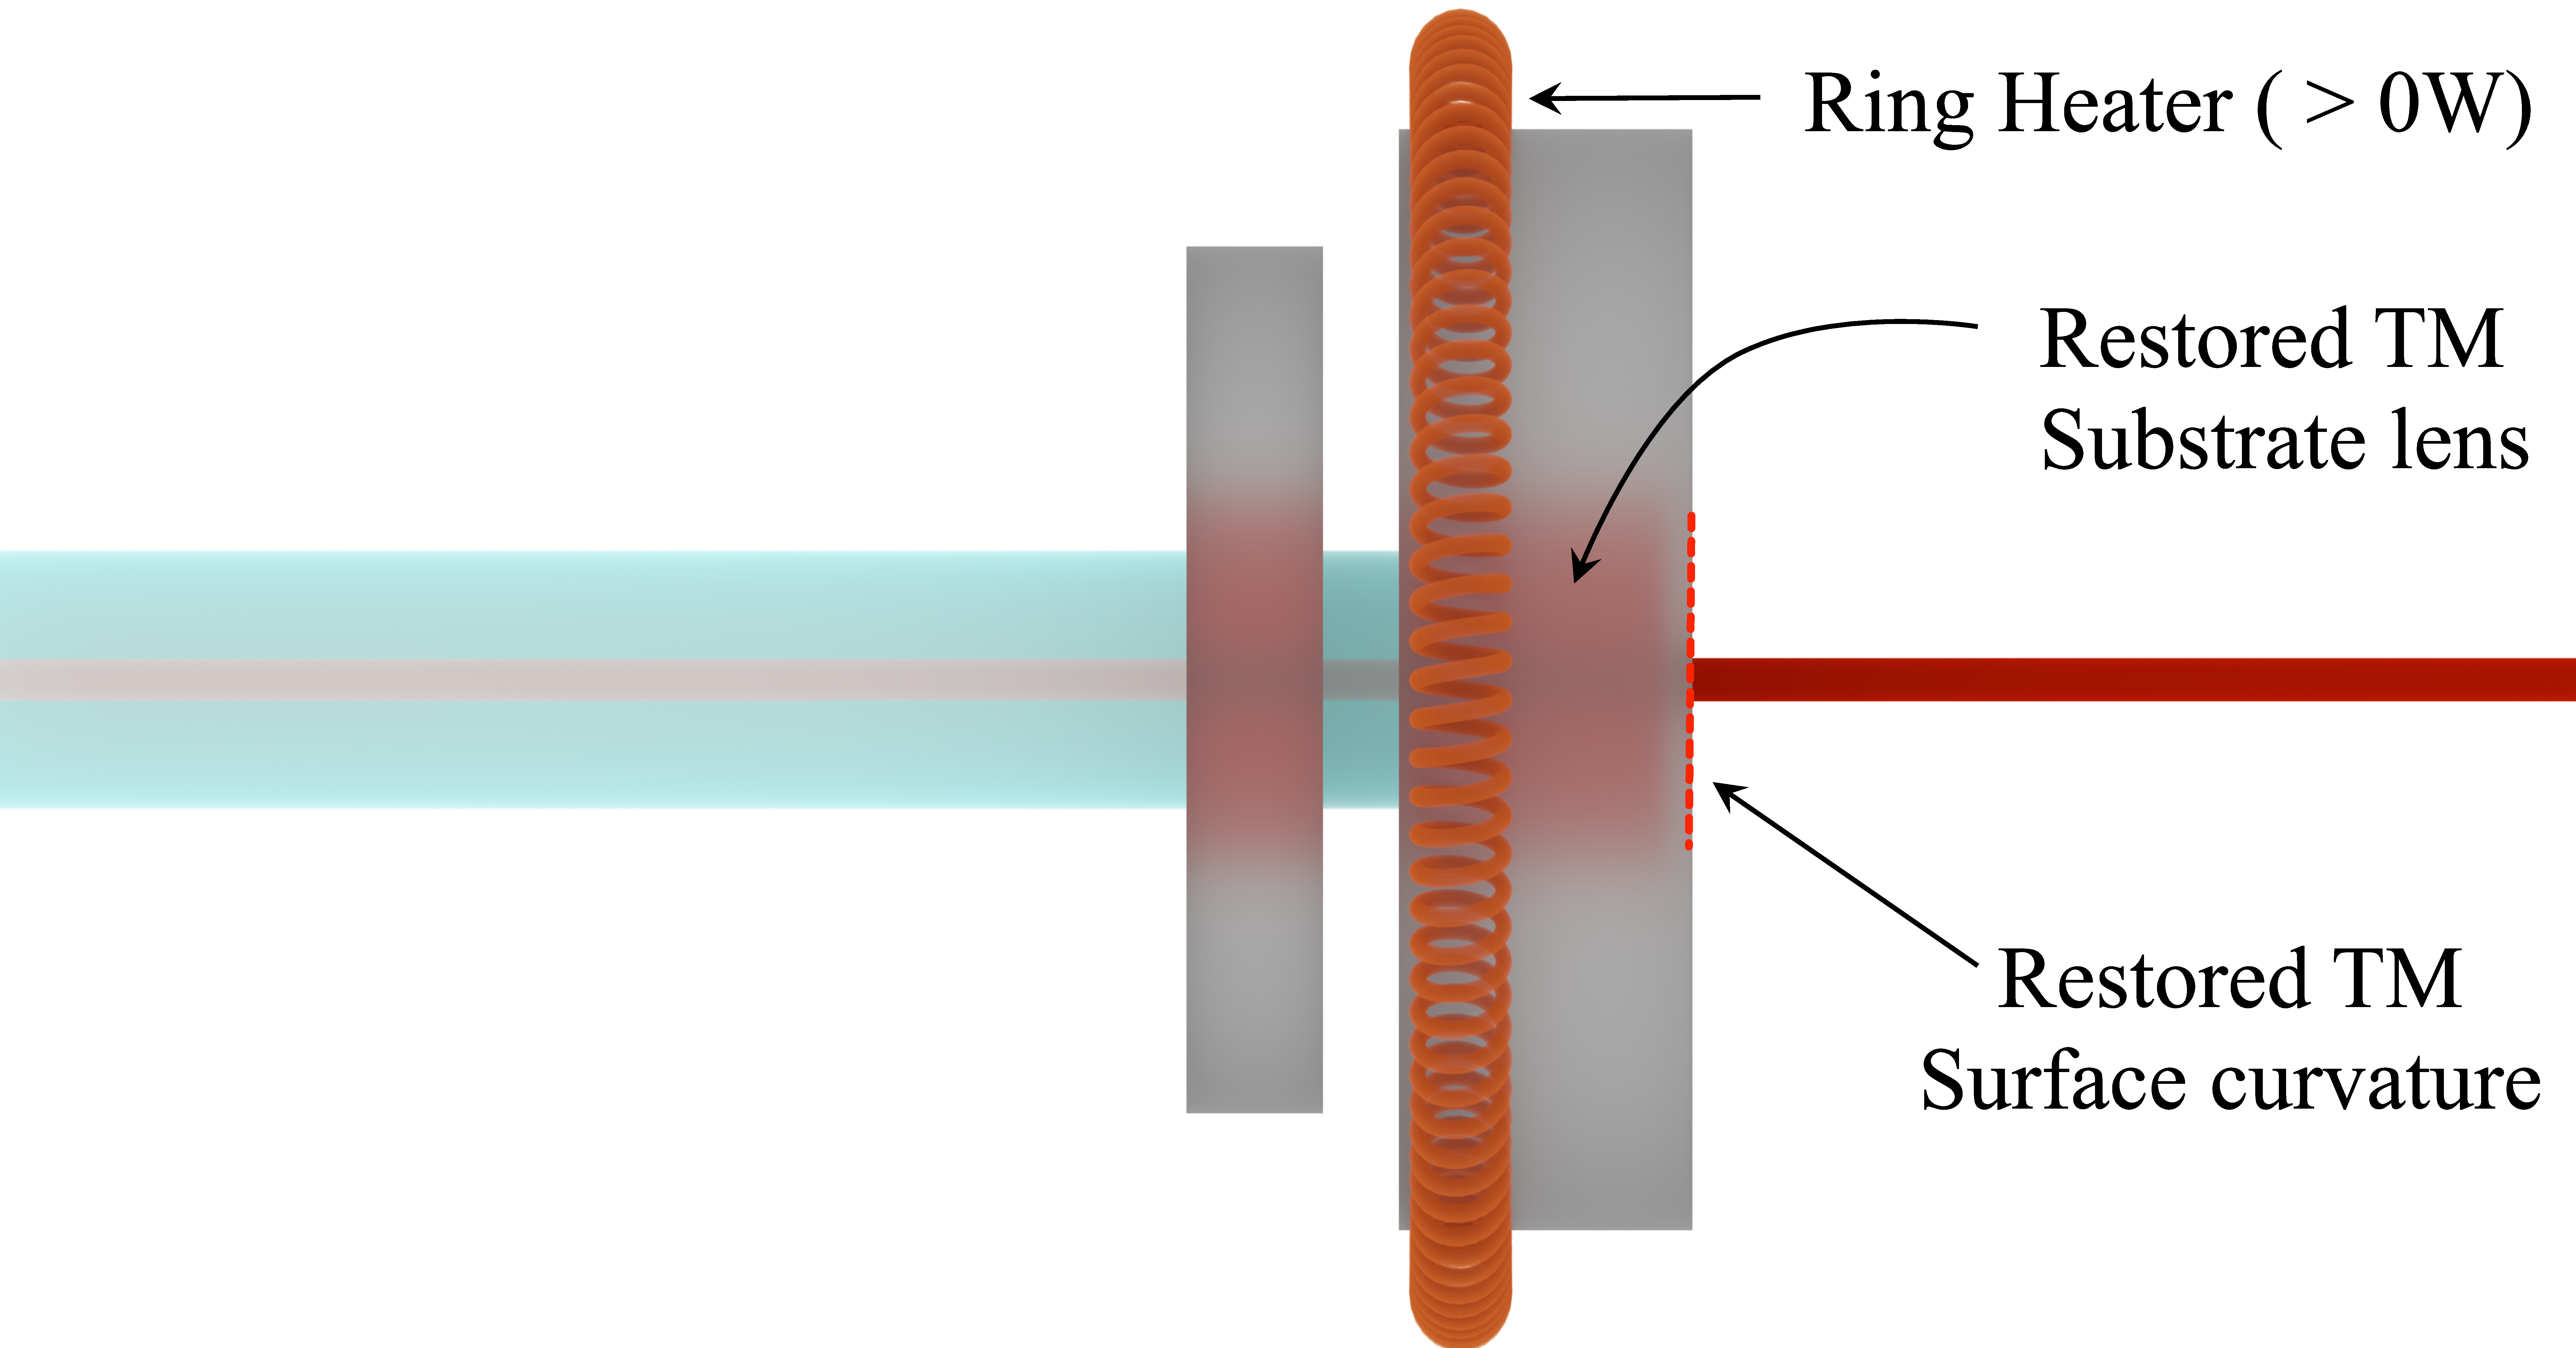
\includegraphics[width=.6\textwidth]{TCS/ITMYarminp/annotated/max/ITMYinp_highcirc.pdf}
		\caption{Maximum circulating arm power, with annular heating and no central CO2 actuation. The careful timing and calibration of the CO2 / RH actuators allow designed power / GW detector sensitivity to be reached.}\label{subfig:TCSinp_highcirc}
%		\caption{Maximum circulating arm power, with annular heating and no central CO2 actuation. The careful timing and calibration of the CO2 / RH actuators allow designed power / GW detector sensitivity to be reached.}\label{TCSinp_highcirc}
	\end{subcaptiongroup}
	\caption{ALIGO thermal compensation design at the input of a single Fabry-P\'{e}rot arm cavity. Though not the only location of thermal mode matching actuators, a careful look here can adequately demonstrates their capabilities and motivates their careful tuning while comissioning the current generation of gravitational wave detectors at high power.}
	\label{fig:meas}
\end{figure}

The gaussian beam 

\section{A priori TCS pre-load methodology for O3a}
Preserving arm cavity resonances requires countering the positive thermal lens defocus of the nominal test mass lens induced by high circulating interferometer arm cavity power. Preparing for this central uniform test mass distortion from the carrier beam requires calibrated and well established thermal actuator settings which in turn informs how much to `pre-load' the TCS actuators using early estimates of test mass absorption. Initial order of magnitude estimates of wavefront distortion from ultra-low absorption fused silica test masses under the influence of a centered high power gaussian beam as well as annular ring heater actuation are available \cite{hellovinet:1990, ramette:2016}; though variations of the absorption between any two test mass mirrors are accounted for through calibrated defocus measurements using the Hartmann wavefront sensors sensitive to auxilary beams imaged onto the test mass mirror surfaces. Measured wavefront distortion is then mapped in real time to Zernike polynomial coefficients used to compute a differential defocus in diopters.

\subsection{The thermo-optic response}
\begin{figure}[!ht]
  \centering
  \begin{subcaptiongroup}
	  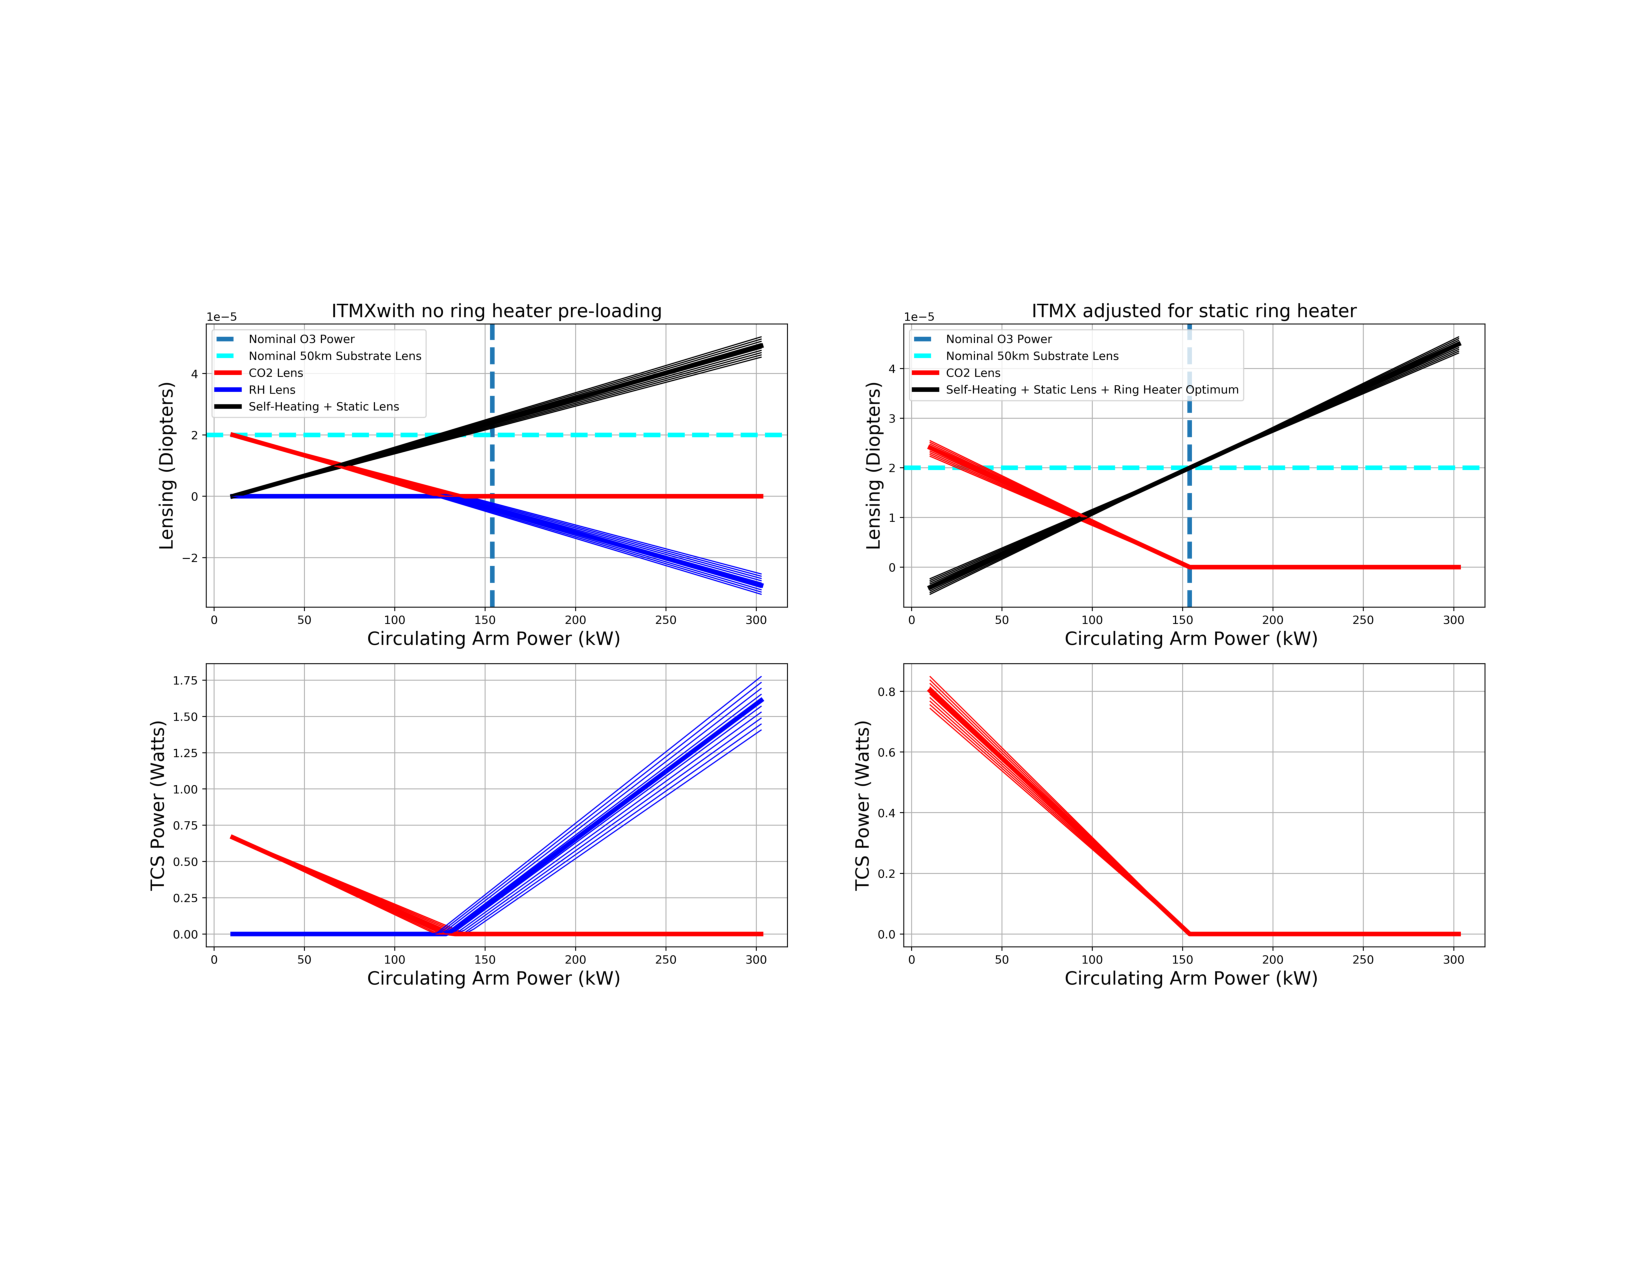
\includegraphics[width=\textwidth]{TCS/ITMX_TCS_Settings_tvo.pdf}
	  \phantomcaption\label{TO_response}
  \end{subcaptiongroup}
  \captionsetup{subrefformat=parens}
  \hfill
  \caption{Measured defocus from the carrier beam self heating and TCS actuation (central CO2 laser heating and annular ring heating.)} 
\label{fig:thermooptic_response}
\end{figure}
The thermo-optic time constant of the central self-heating response is similar to that seen from CO2 central actuation, though demonstrably different from annular ring heating. Because of this, LHO applies the central CO2 heating and static annular ring heating to a power level that respectively mimics and actuates for projected thermal deformation from the high power circulating resonant carrier beam in the Fabry-Perot arm cavities. Once DRFPMI coupled cavities are configured or ``locked'', the input carrier power is gradually increased while CO2 laser powersimultaneously decreased in order to mitigate any possible differential thermo-optic response from the arm cavity test masses when reaching maximum power.
\begin{figure}[!ht]
  \centering
  \begin{subcaptiongroup}
	  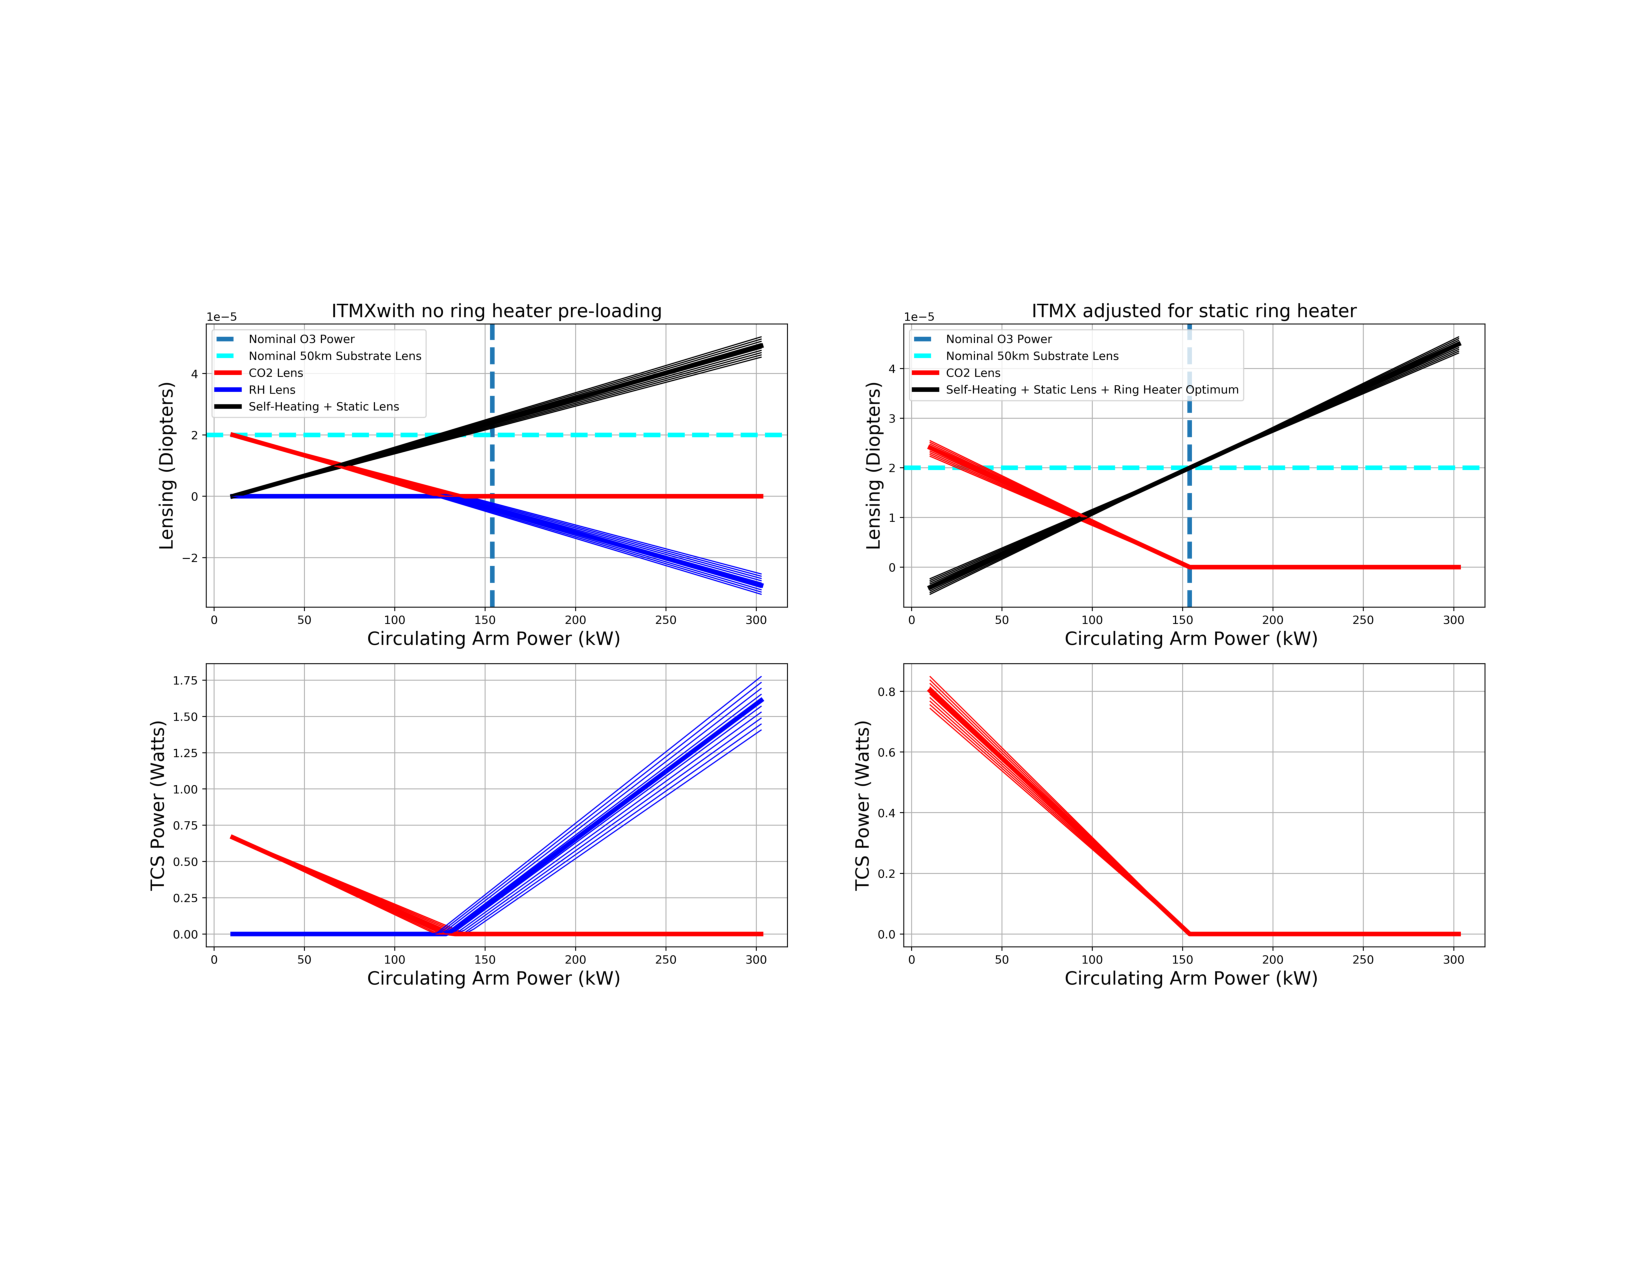
\includegraphics[width=\textwidth]{TCS/ITMX_TCS_Settings_tvo.pdf}
	  \phantomcaption\label{ITMX_TCS}
	  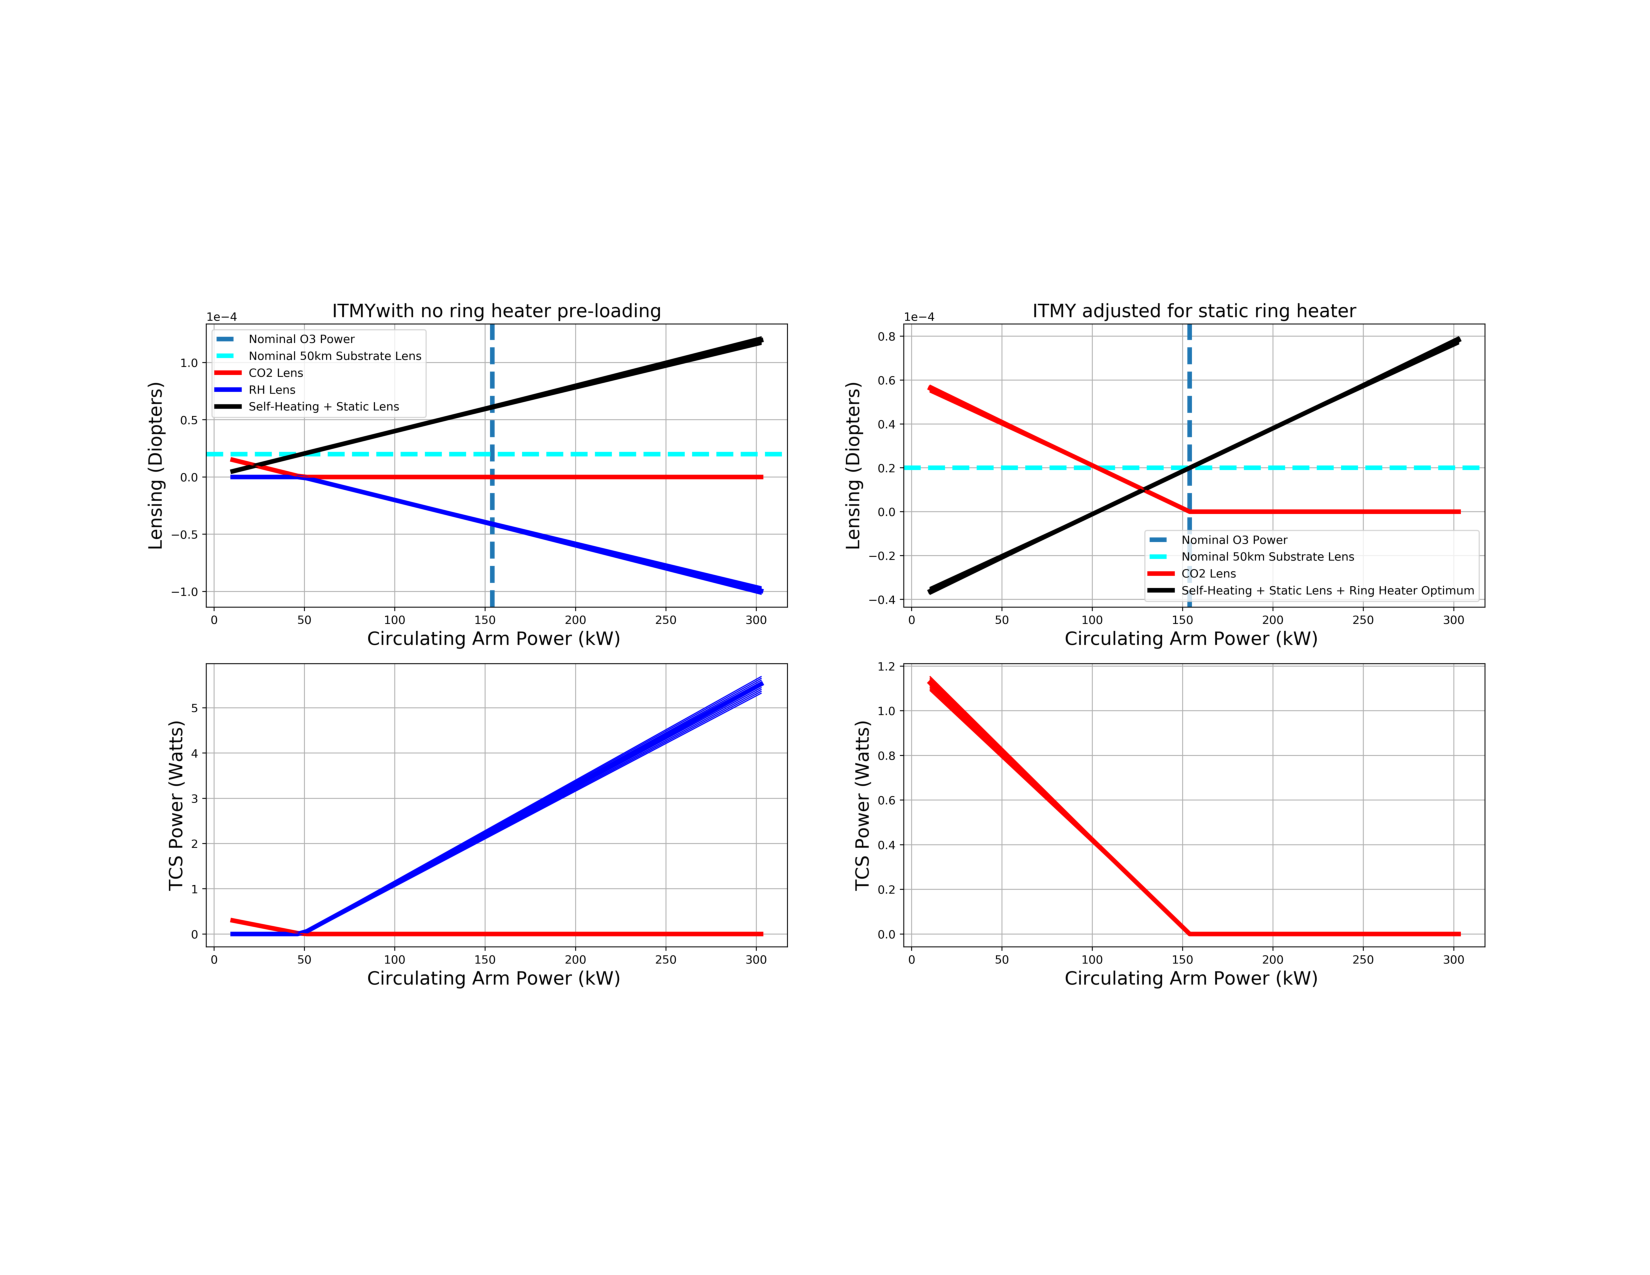
\includegraphics[width=\textwidth]{TCS/ITMY_TCS_Settings_tvo.pdf}
	  \phantomcaption\label{ITMY_TCS}
  \end{subcaptiongroup}
  \captionsetup{subrefformat=parens}
  \hfill
  \caption{The initial pre-load estimates for the ITMs at the LIGO Hanford Observatory for O3a as provided in \cite{tvo}} 
  \label{fig:O3_preload_tvo}
\end{figure}


\section{A posteriori thermal compensation for O3a}
While approaching designed arm cavity power, the presence of non-uniform absorption on the test mass coating surface imposed limits to reaching designed power and hence designed sensitivity; which simultaneously lead to a significant deviation from the original TCS pre-loading algorithm.  Assessment of these absorbers can inform methods of improving detector sensitivity required and initial characterization of these high absorbtion points which includes noting the characteristic optical path distortion as measured on the Hartmann wavefront sensors and the impacts on interferometer operations especially at high power. Current thermal actuation solutions are currently designed to control the TEM00 beam waist size and location though adjustments and modifications of current actuators was tried. This summary indicates that these absorbers may impose a barrier to maintaining high power in the arm cavities if no further proactive measures are not taken or are not sufficient to bypass detector symptoms; whether they are a result of preventable surface particulates or improved higher frequency.  

%The presence of high absorption points on the test masses (aka point absorbers) required adjustments to the TCS pre-load and various ring heater and CO2 settings were sampled. Part of this sampling lead to the development of a input ring heater filter allowing actuation to reach ? percent of the desired optical power within 2 hours compared to the 12 hour response pre-filter. Higher spatial frequency actuation in the form of a CO2 mask was also tried.

\subsection{Point absorbers in O3a}
\subsubsection{ITMY absorbers}
\begin{figure}[H]
  \centering
  \begin{subcaptiongroup}
	  \includegraphics[width=.495\textwidth]{TCS/PA/ITMY_absorbers.pdf}
	  \phantomcaption\label{subfig:itmypajustself}
	  \includegraphics[width=.495\textwidth]{TCS/PA/ITMY_self.pdf}
	  \phantomcaption\label{subfig:itmypaselfplusabs}
  \end{subcaptiongroup}
  \captionsetup{subrefformat=parens}
  \hfill
  \caption{An isometric view of uniform absorption vs point absorption of LHO ITMY}
  \label{fig:ITMYpabs}
\end{figure}

\subsubsection{ETMX absorbers}
\begin{figure}[H]
  \centering
  \begin{subcaptiongroup}
	  \includegraphics[width=.49\textwidth]{TCS/PA/ETMX_absorber_short_heat.pdf}
	  \phantomcaption\label{subfig:etmxpajustself}
	  \includegraphics[width=.49\textwidth]{TCS/PA/ETMX_absorber_full_heat.pdf}
	  \phantomcaption\label{subfig:etmxpaselfplusabs}
  \end{subcaptiongroup}
  \captionsetup{subrefformat=parens}
  \hfill
  \caption{An isometric view of uniform absorption vs point absorption of LHO ETMX. The rippling / edge effects are a consequence of the Hartmann probe beam experiencing unavoidable clipping on the baffle due to misalignment of in-vaccum optics.}
  \label{fig:ETMXpabs}
\end{figure}

Impact on interferometer contrast and transmission / co-resonance of higher order modes

\subsubsection{Impacts}
A significant number of lockloss events during the comissioning period for O3A when increasing detector input power were a direct result of select optical sideband power degredation used to maintain the delicate coupled cavity configuration. And while sustaining interferometer DC readout the arm cavity would generate higher order modes sustained by Output Mode Cleaner (OMC) co-resonance; contaminating the carrier field at the output photodiode.

\paragraph{Controls schema}
\textcolor{red}{Sensor schema for interferometer control and dramatic impact to optical sidebands (higher order beat signals)}
\paragraph{Frequency noise}
\paragraph{Parasitic higher order modes}
Visible higher order modes at the anti-symmetric port \\
A significant amount of optical loss as a result of losing sideband power is reported \\
	* Lockloss caused by reduced sideband power with interferometer thermalization \\

\subsubsection{Attempted symptom reduction}
The trivial solution of reducing the test mass non-uniformity was tried but exhibited noticable limitations with the available degrees of freedom. To restore the uniformity of the test mass surface, a custom mask was constructed with the intention of imaging a negative of the optical path distortion high absorption points onto the surface with the CO2 laser combined with a static ring heater offset. 

The installation location of the mask and size was established using the relevant propogation and imaging tensors applied to the CO2 actuation field while mitigation of the aforementioned impacts provided comissioners with the notable metrics of success.

\textcolor{red}{Results}
\\
The extremely strict alignment requirement introduced difficulties while attempting to fulfill the promise of restoring uniform absorption. And although the presence of the absorber symptoms show coorelation with their prominence at high power, their collective reduction proved not to be as straightfoward~\cite{brooks:aigwd2019, buikema:2020}.
	
	* CO2 with enhanced focus on absorbers and ring heater actuation
		* Very narrow alignment requirement
		* Improvement metrics
			* Restoring sideband power	
	* Adjusting interferometer to OMC mode matching
		* Improvement metrics:
			* Reduced HOM content at detector output
			* Tracking dither line amplitudes

%\begin{figure}[H]
%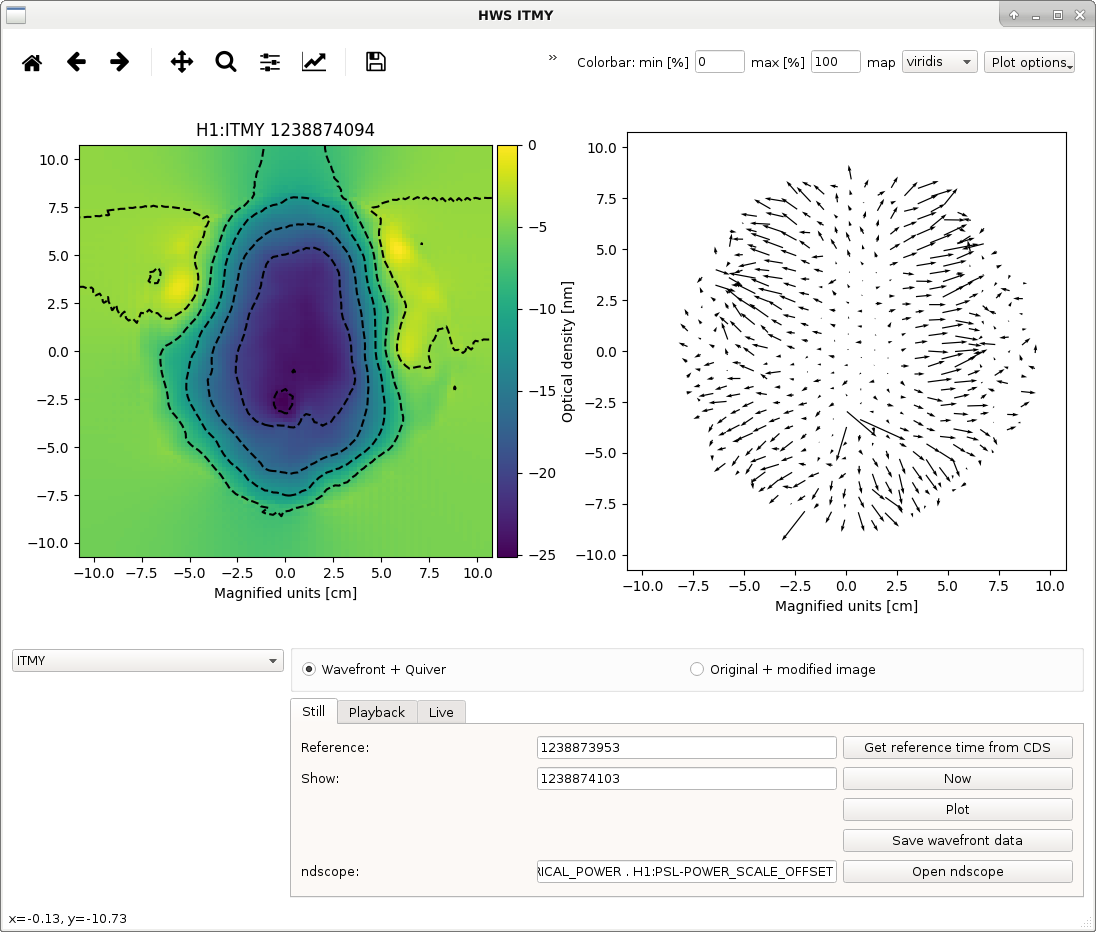
\includegraphics[width=\textwidth]{figs/TCS/PA/48349_20190409201649_inital_install_CO2Ymask2_150seconds_900mW.png}
%\caption{Point absorber figure with second $\mathrm{CO_2}$ mask}
%\label{fig:RH_power}
%\end{figure}

\section{Dynamic Thermal Compensation}
\subsection{A closer look at the ring heater / test mass thermo-optic response}
Transient ring heater actuation from a radially symmetric thermal aberration ($\Psi(t,r)$) is realized ~\cite{ramette:2016}:
\begin{equation}
	\Psi(t,r)=2\frac{dn}{dT} \sum^{\infty}_{m,p = 1} A_{m,p} \; c^{u}_{p} \mathrm{sin}(u_m h /2a) (a/u_m)[1-e^{-\alpha t}] J_0(\zeta_p r/a)
\end{equation}

\begin{figure}[H]
     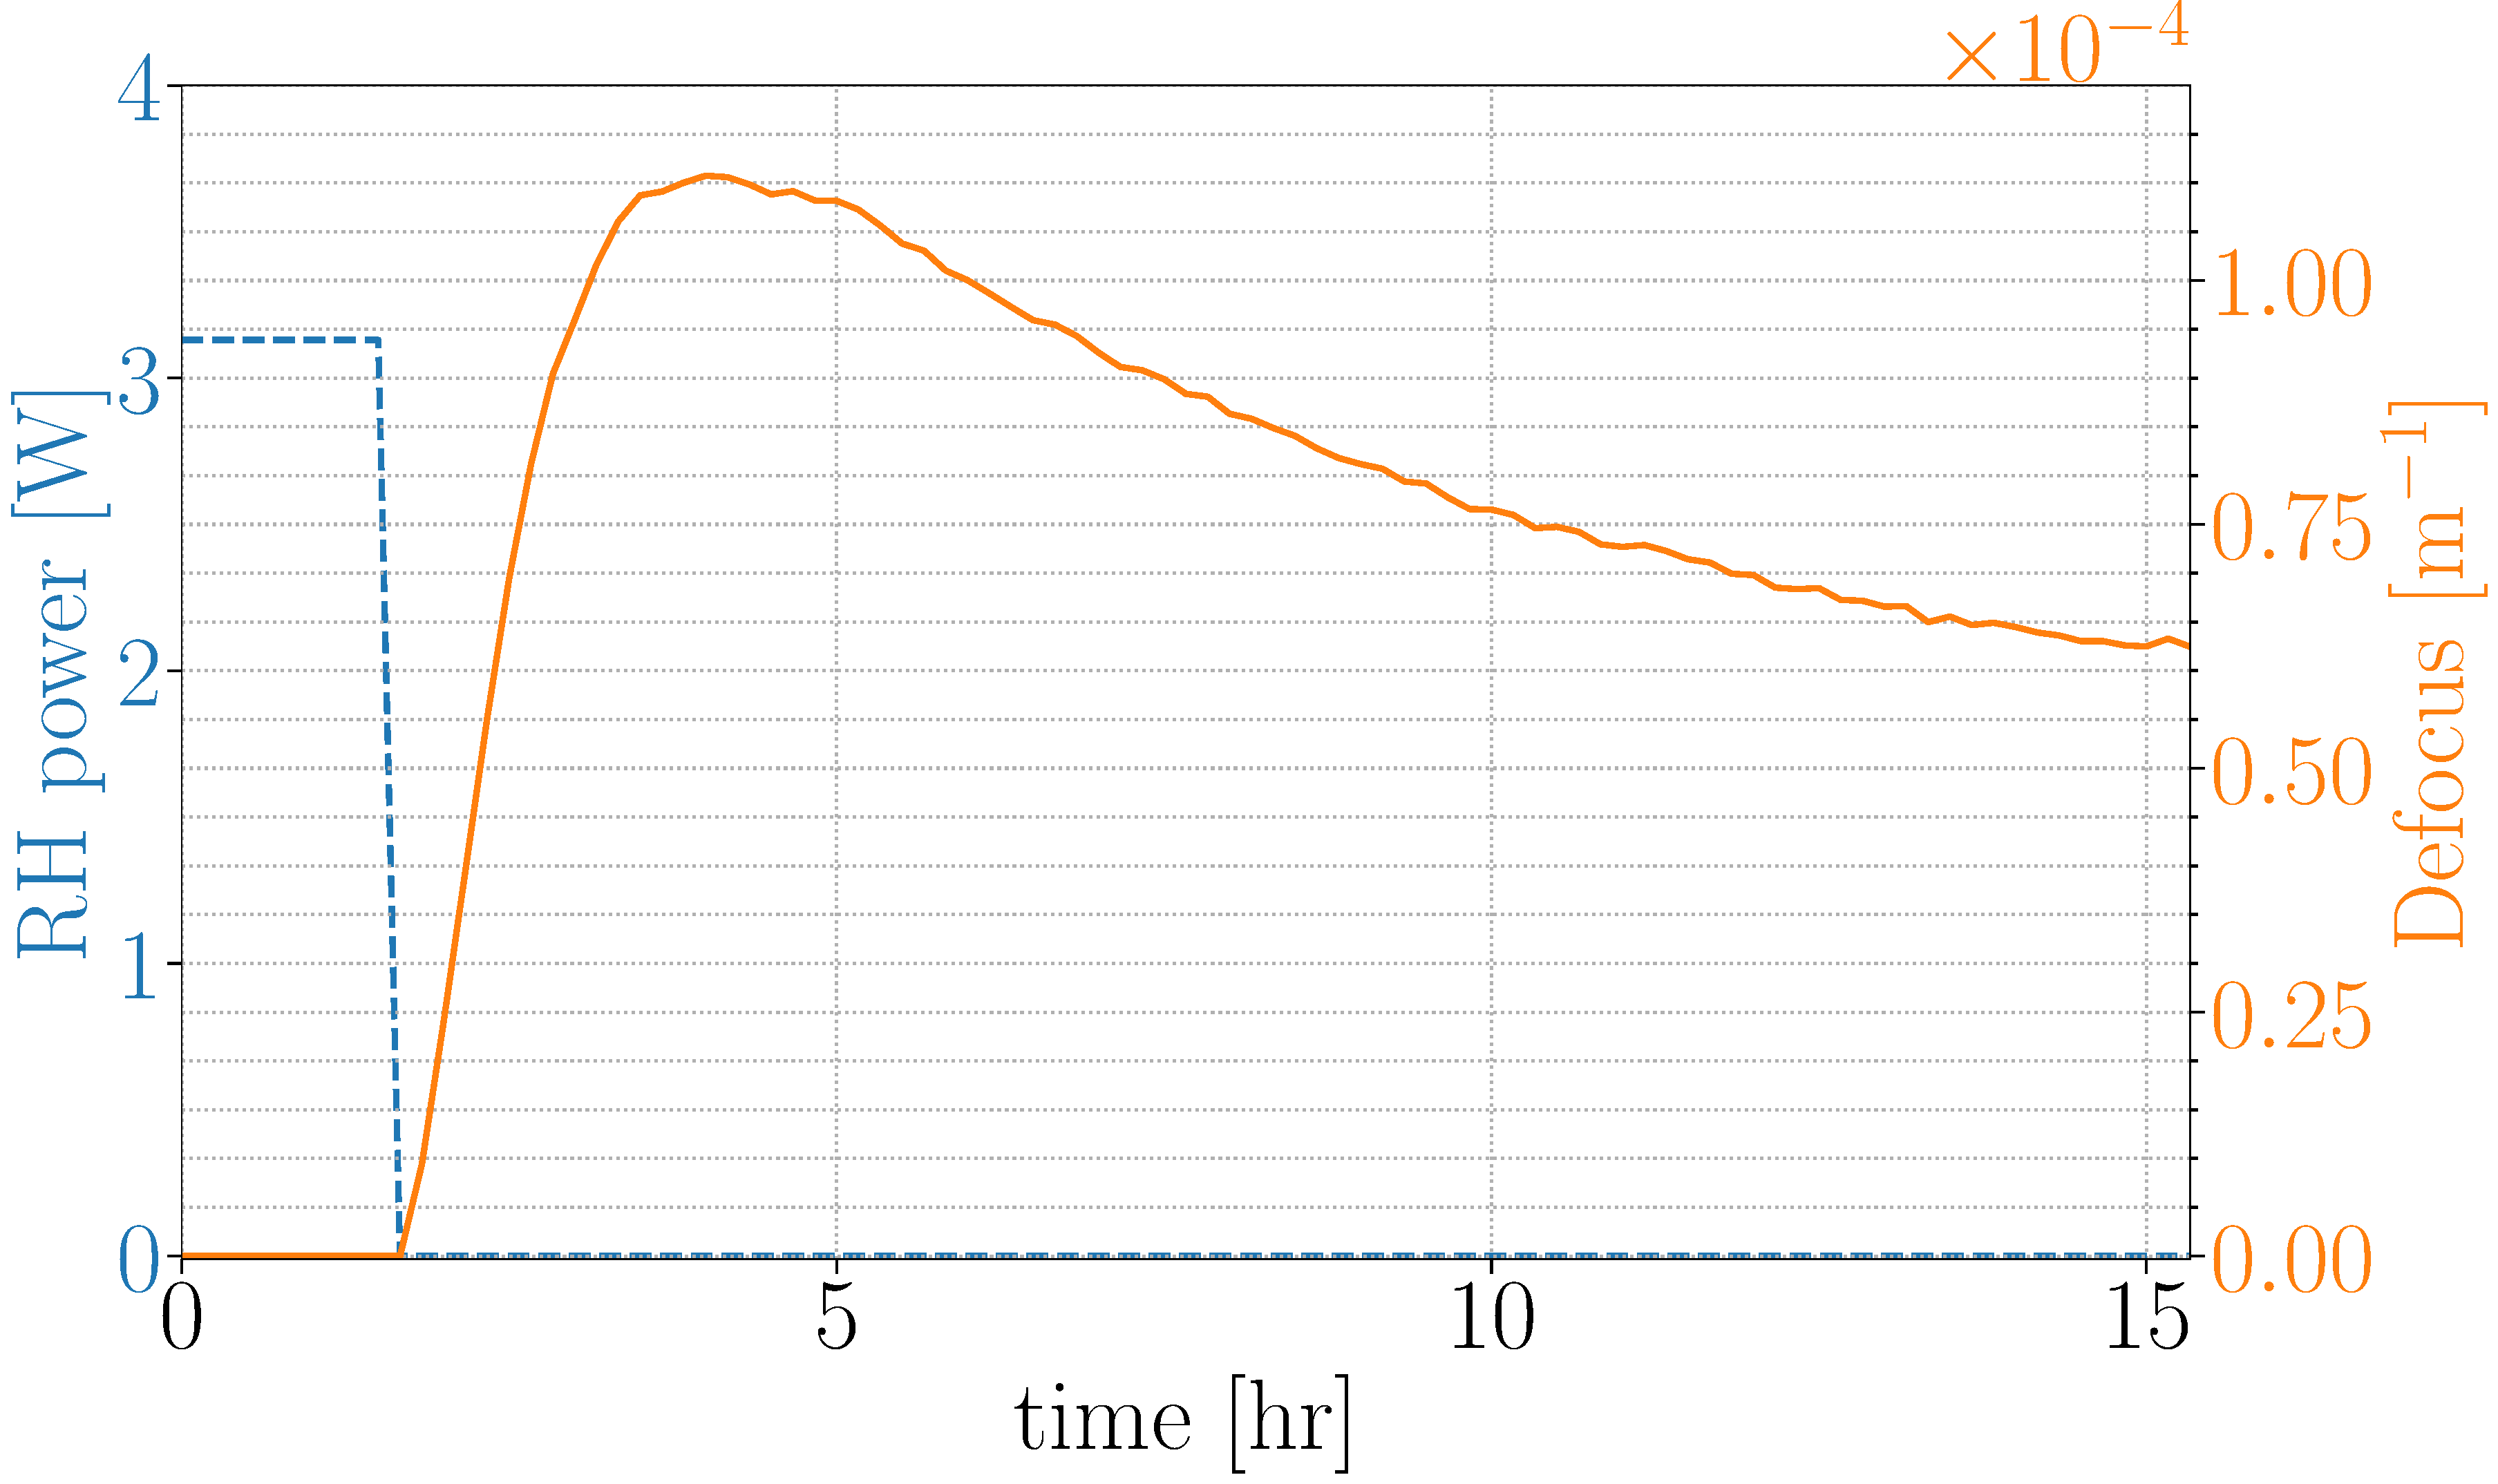
\includegraphics[width=\textwidth]{TCS/IRHF/Meas_response}
     \caption{ITMY thermo-optic response to a 3.13 [W] combined power reduction to the top and bottom ring heater elements. It's after $\approx$ 12 hours after the ring heater power control step do you start to see a small enough steady state differential defocus ($\frac{\mathrm{d} \alpha_\mathrm{sp}}{\mathrm{dt}}$) and can assume a steady state thermal lens.}
     \label{fig:RHresp}
\end{figure}

The measured thermo-optic step response exhibits differential defocusing for $\approx$ 12 to 15 hours once the ring heater power has been changed; and with a large enough power steps, these adjustments to ring heater power can significantly stall precious detector observing/comissioning time from the differential mode matching conditions in the DRFPMI. This thermo-optic time constant can be reduced by applying a real time digital filter to the ring heater power control. The desired thermo-optic response is one that resembles a step from one defocus state to another with no intermediate overshoot. 

\begin{figure}[H]
    \centering
    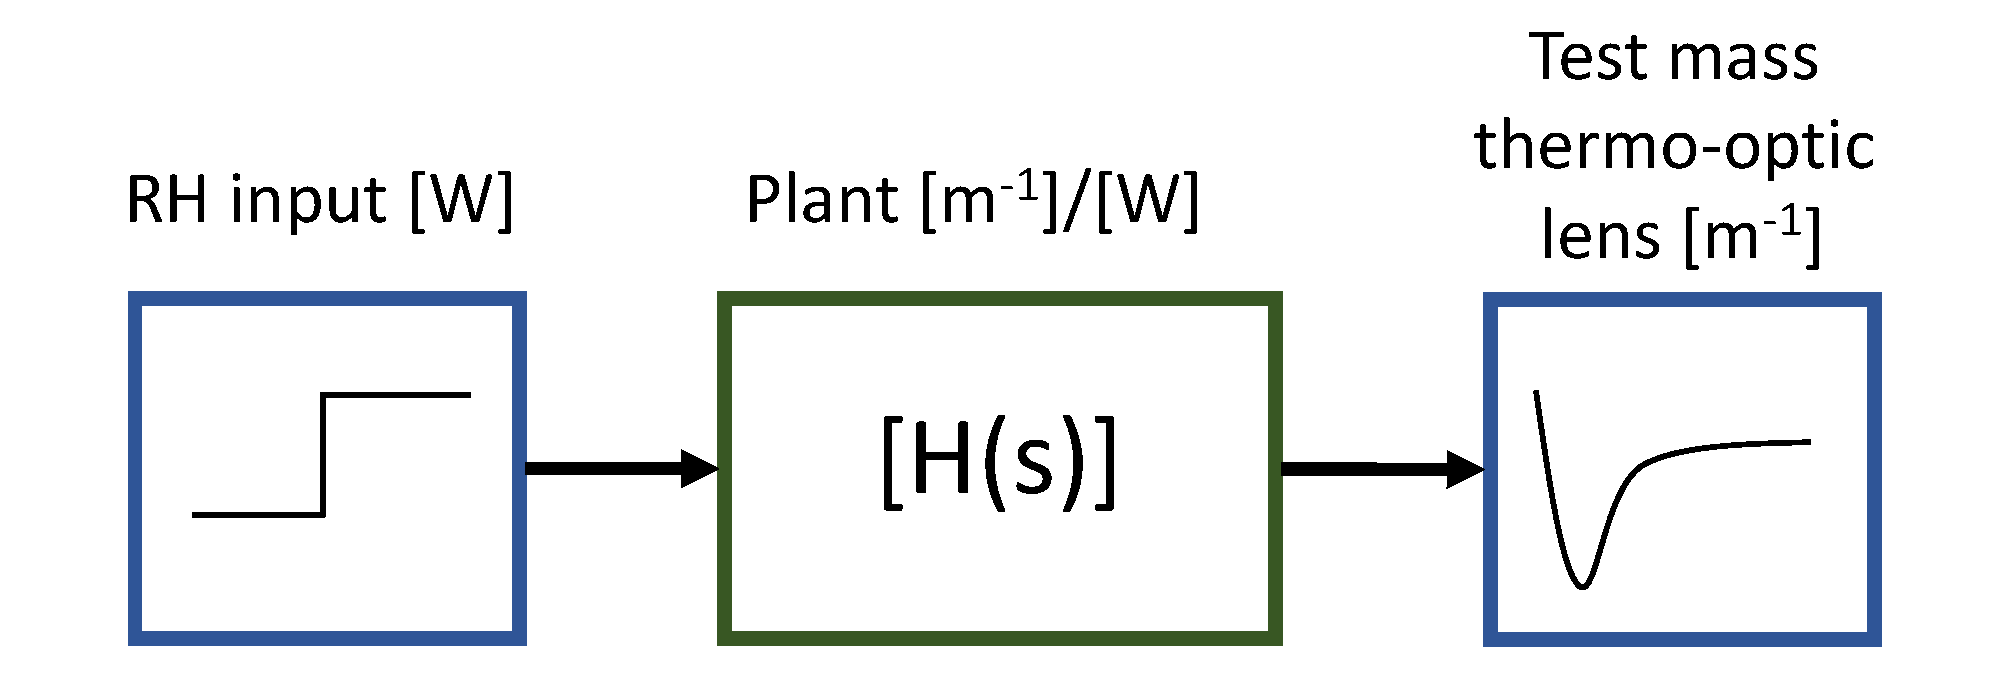
\includegraphics[page=1,width=.75\textwidth]{TCS/IRHF/RH_input_filter_figures.pdf}
    \caption{A feedback-style block pictograph of the plant system (test mass mirror and annular ring heater) transforming the ring heater power control step to a time-varying thermo-optic response. The example of this can be seen in Fig [\ref{fig:RHresp}]}
    \label{fig:justplant}
\end{figure}

The prescription for creating such a filter is realized through the inversion of the well known step response, alongside additional low passing at high frequency to avoid any control instabilities at high frequency.

\textcolor{red}{see appendix for more detail}
%\begin{enumerate}[label=\arabic*),leftmargin=75pt,nosep]
%	\item Fit step response to a zpk filter $H(s)$ 
%	\item Invert fitted filter ($H(s) \rightarrow H^{-1}(s)$) 
%	\item Apply correction filter $G(s)$ for stability and speed tuning ($H^{-1}(s)*G(s)$)
%\end{enumerate}

\begin{figure}[H]
    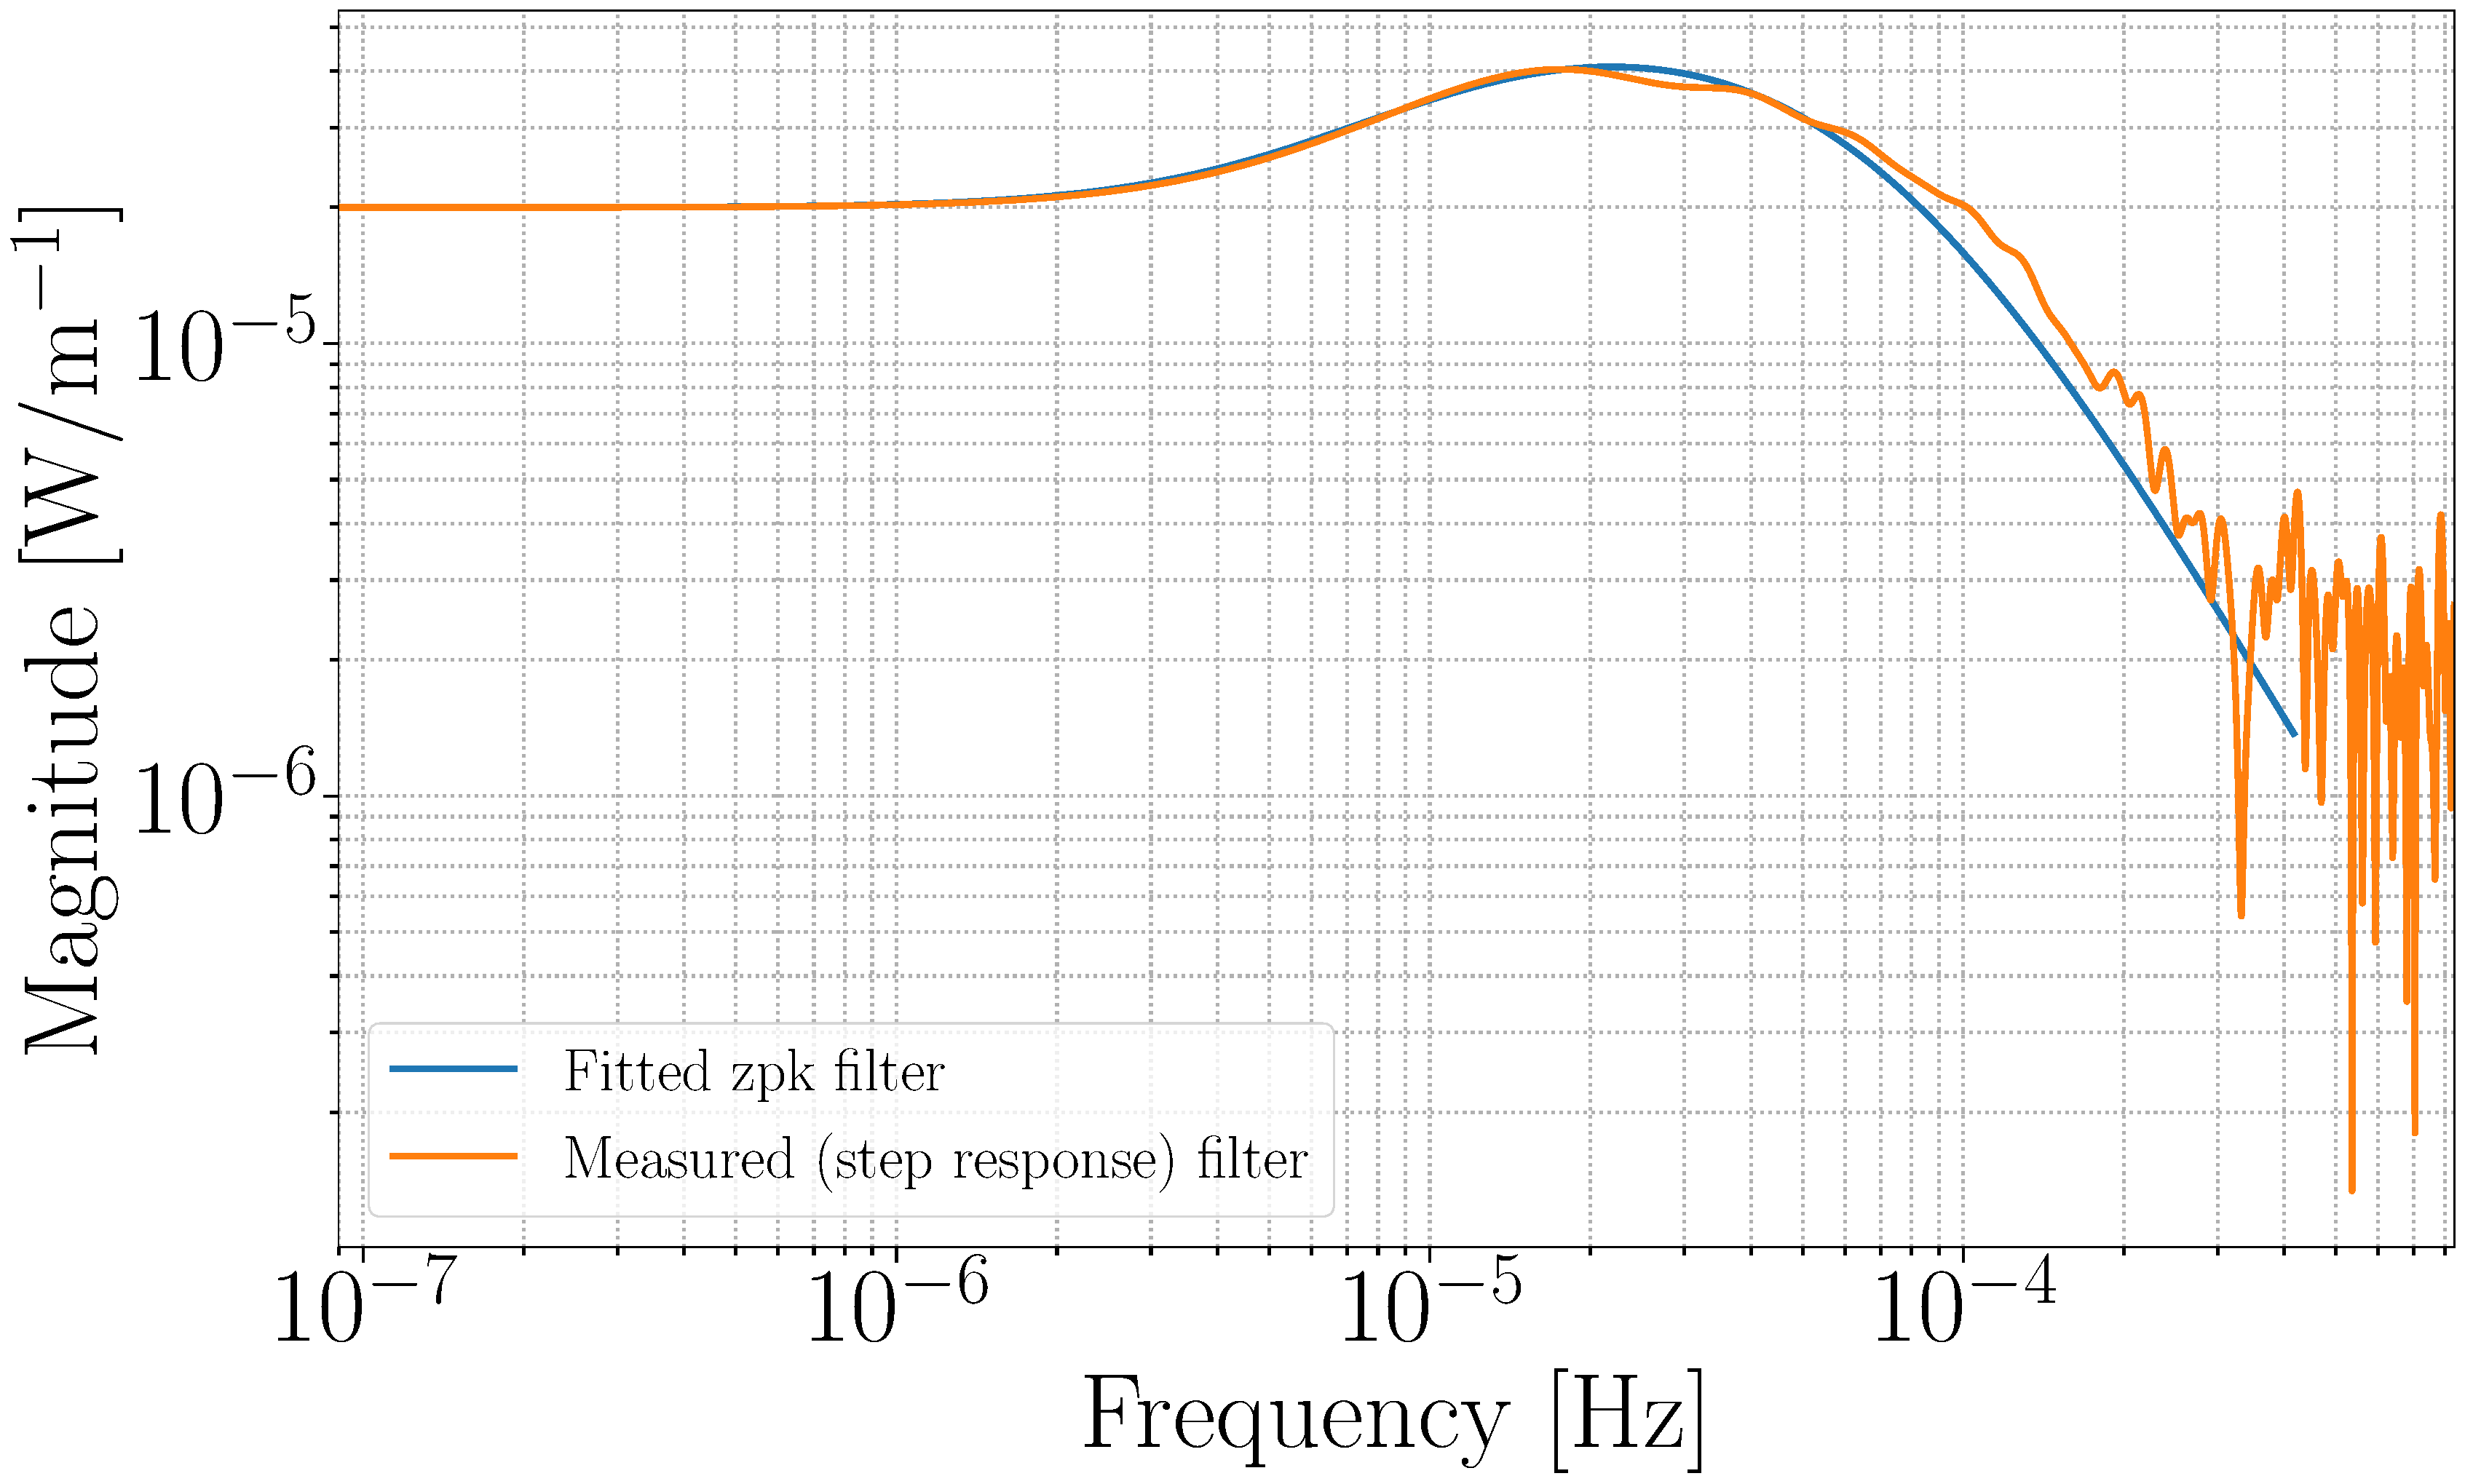
\includegraphics[width=\textwidth]{TCS/IRHF/RH_plant_filter_fit}
    \caption{Showing the PSD of the RH response (normalized by the input RH power) over a an $\approx$ 12.5 hour period. The zpk model of the fitted filter (H(s)) is $9.2545e-12 \frac{(s+3.14210e-5)}{(s+8.168e-5)(s+0.0003142)(s+0.0005969)}$}
    \label{fig:plant_v_fit}
\end{figure}

\begin{figure}[H]
    \centering
    \includegraphics[page=2,width=.9\textwidth]{TCS/IRHF/RH_input_filter_figures.pdf}
    \caption{A pictograph showing the system with real time digital filtering for an improved thermo-optic response. The RH input filter is created by inverting the plant filter combine with a low pass and added poles to the zpk model to ensure stability.}
    \label{fig:rtdf_pictograph}
\end{figure}

\begin{figure}[H]
    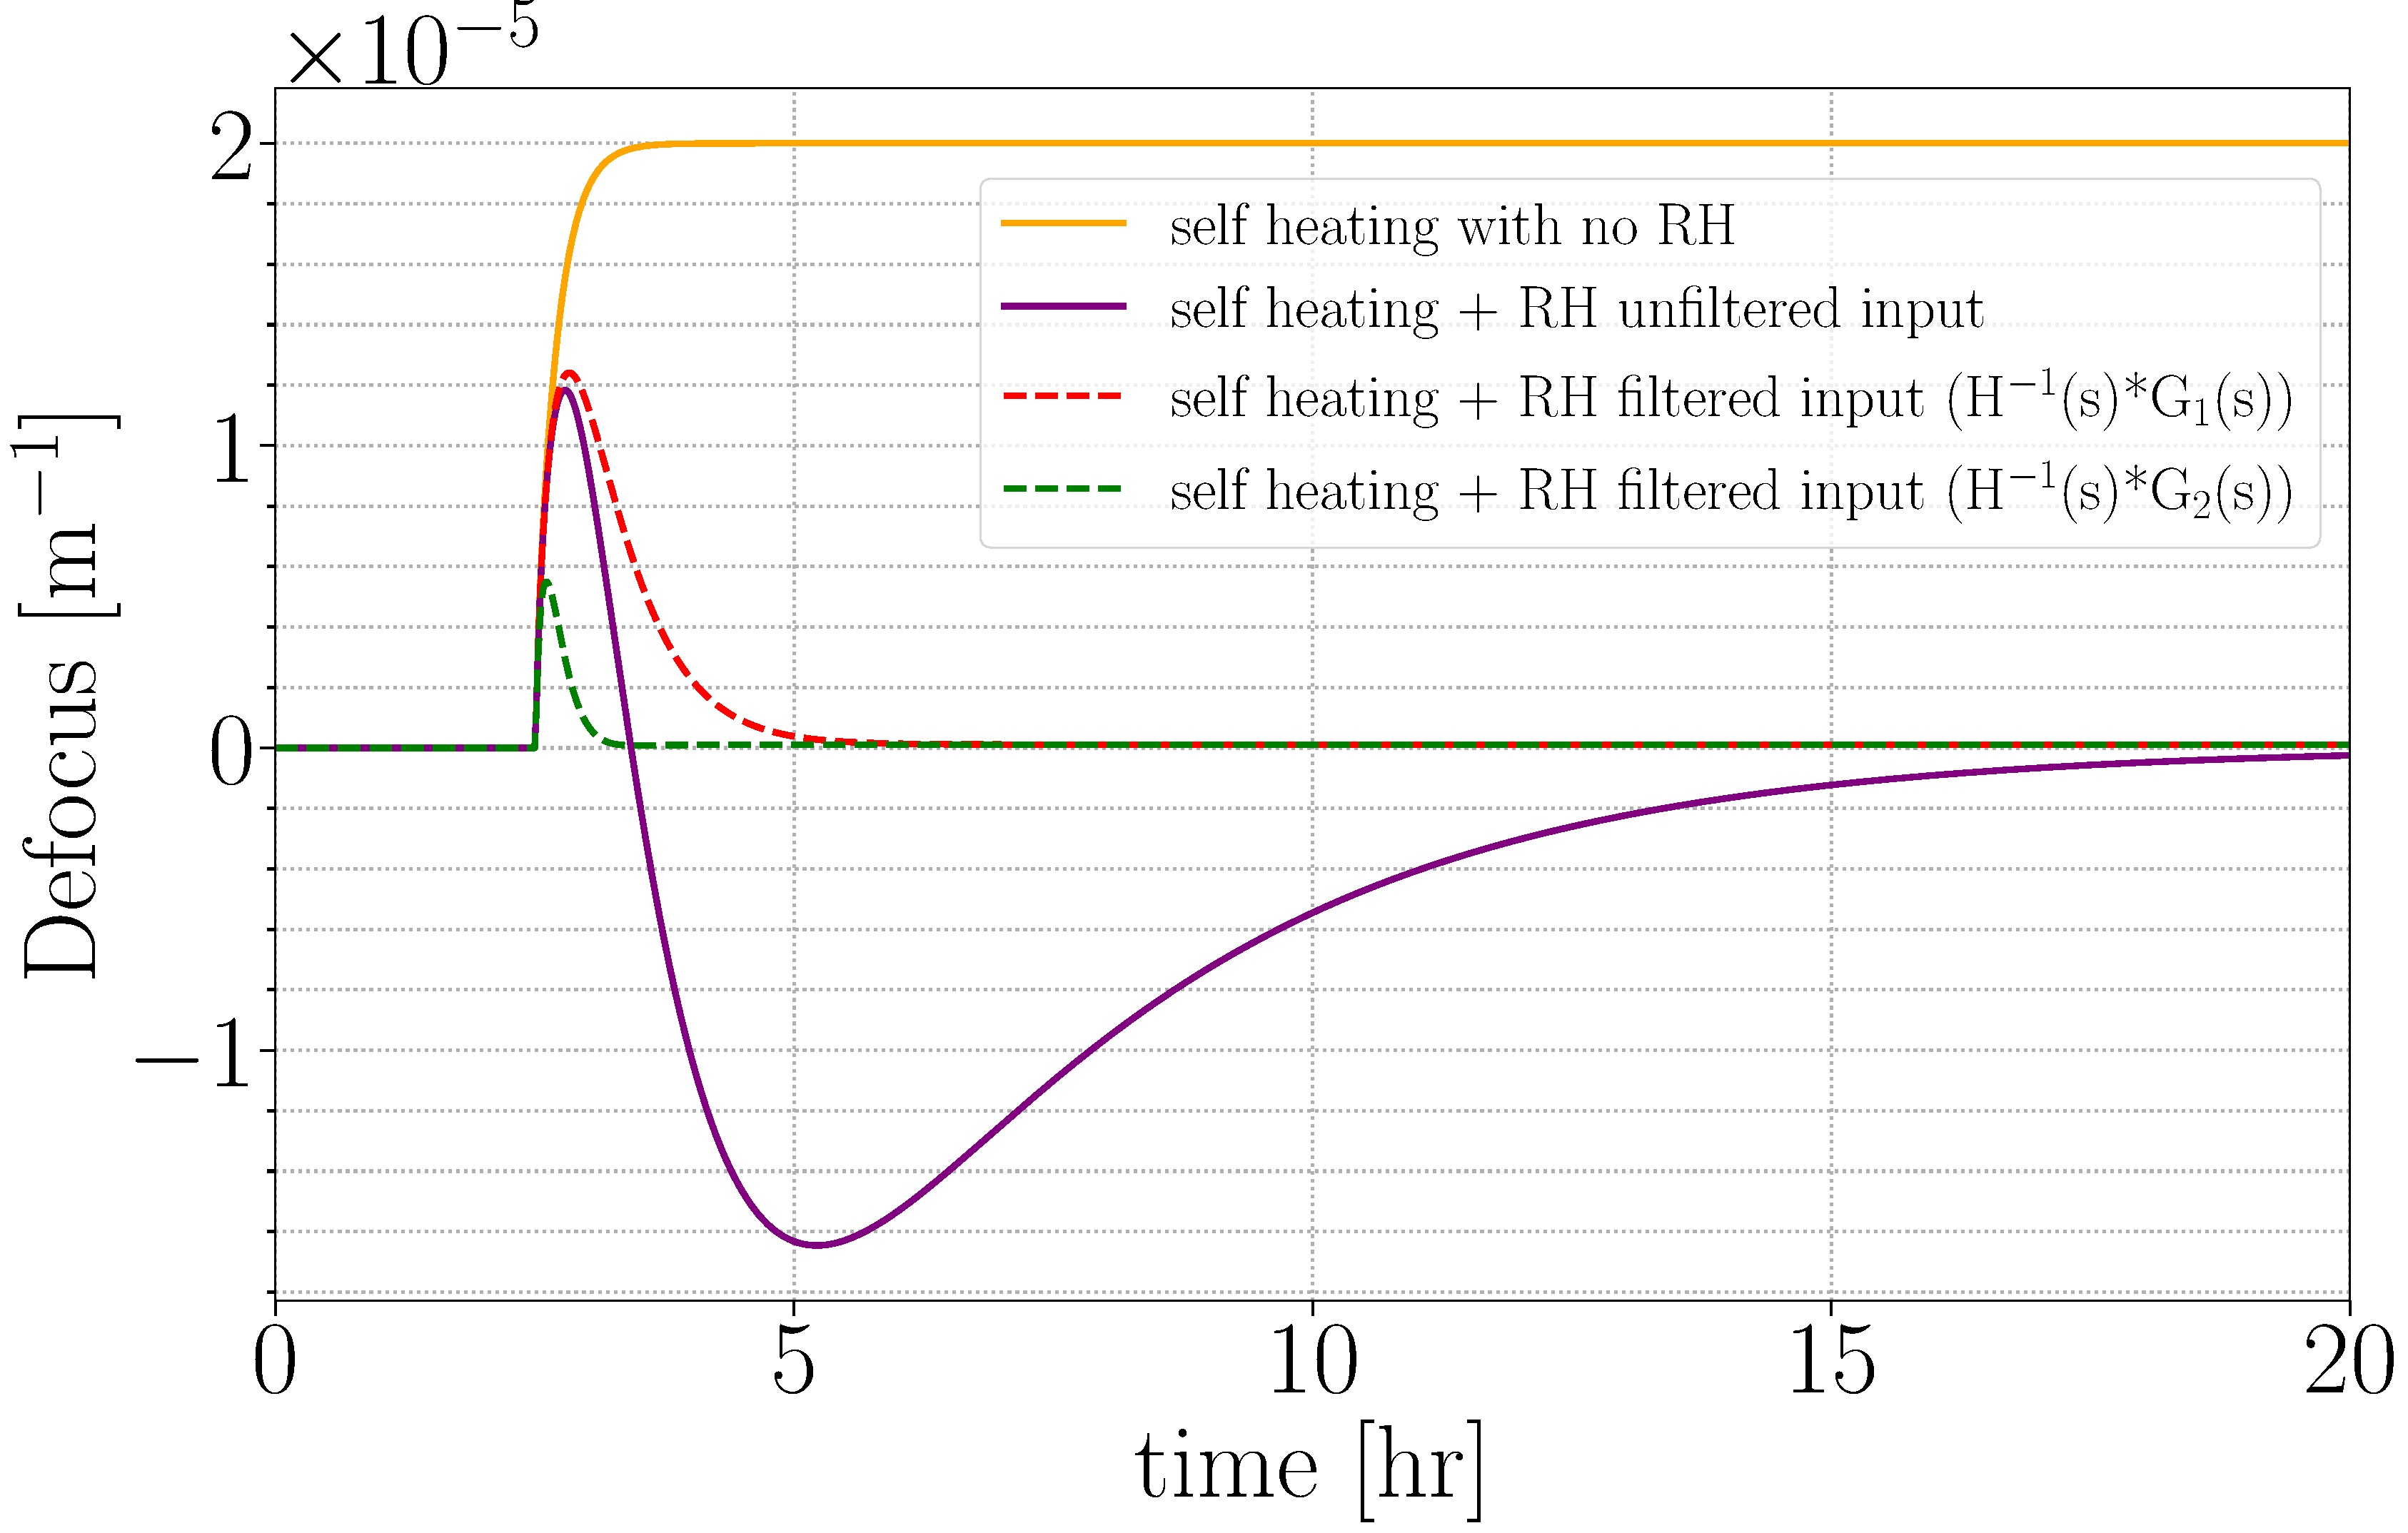
\includegraphics[width=\textwidth]{TCS/IRHF/IRHF_compare_w_self}
    \caption{Comparison of the natural RH response and the response to the conditioned input. The above plot is simulated in Matlab by passing the RH input time series (top plot) through the $[H(s)]^{-1*}$ and $H(s)$ to acquire with the result lensing behavior on the bottom plot.}
    \label{fig:dynam_comparison}
\end{figure}
\newpage

\subsection{Reducing Parametric Instabilities}
Another symptom of resonant high power optical cavities are parametric instabilities (PI); induced by the opto-mechanical interaction between test mass acoustic modes and higher order optical modes. These PIs present threats to achieving designed detector sensitivity, even driving the detector to lockloss. Passive methods of mitigating PIs by way of acoustic mode dampers (AMD) demonstrate significant reductions of problematic mechanical modes though some (i.e. @ 15 kHz mode) have remained problematic. Lingering parametric instabilities required manual intervention by way of adjusting test mass / cavity geometry to disrupt these persistent PIs, and is now a much more feasible solution with DTC \cite{hardwick:2020}.  

\subsubsection{Limitations}
    \begin{figure}[H]
    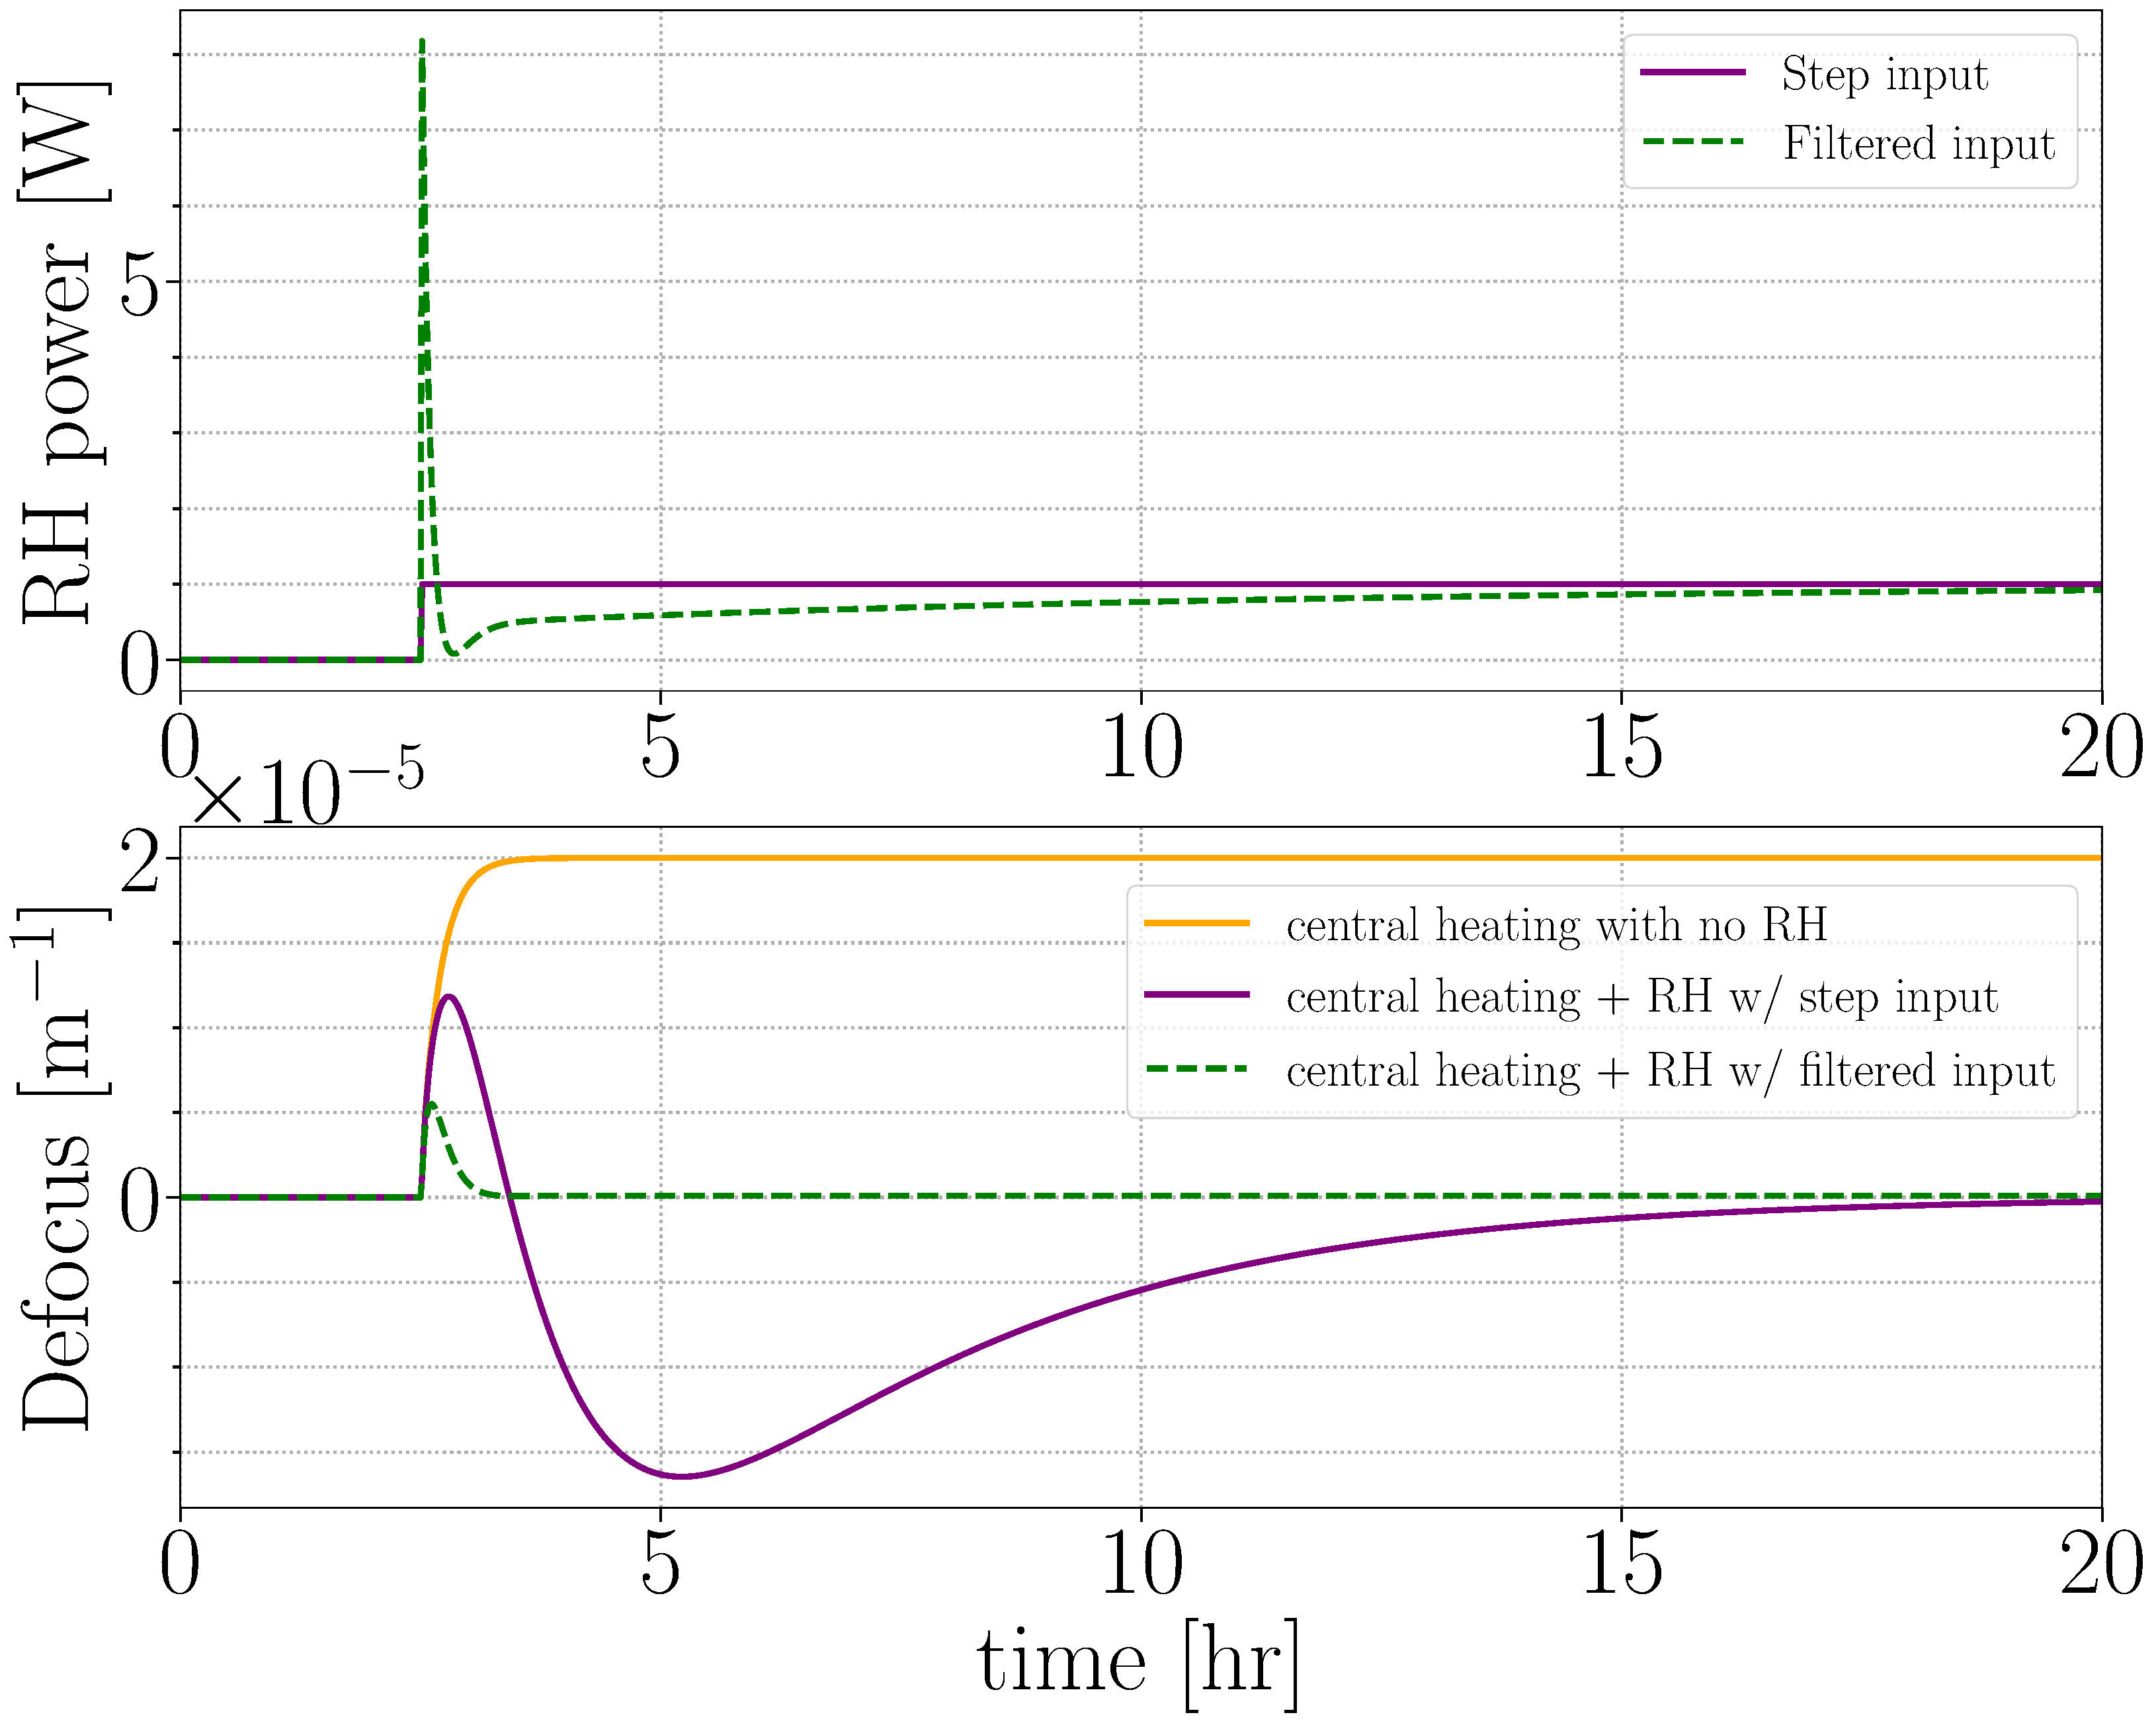
\includegraphics[width=\textwidth]{TCS/IRHF/IRHF_compare_filts_PI_paper}
    \caption{Comparison of the natural RH response and the response to the filtered input with RH power}
    \label{fig:RH_power}
\end{figure}
Limitation on RH power is set at 8W \textcolor{red}{Double check source?}




\chapter{Electro-optic study of an  GaAs/\textbf{AlGaAs} coated sample}
%Electro-optic study of AlGaAs coated mirrors

Once mirror coating materials are selected for DRFPMI core optics, another fundamental detector noise limit (like that discussed in \ref{sec:shot_noise} is imposed on the gravitational wave detector in the form of coating thermal noise. For aLIGO $\siotao$ coatings this is represented in \hyperref[sec:ligo_noise]. As aLIGO approaches designed sensitivity, alternative mirror coating solutions are proposed with the primary purpose of pushing down the thermal noise limit for further enhancing detector sensitivity \cite{?}. With the potential to reduce coating Brownian noise by a factor of 10, $\gaas$/$\algaas$ shows promise for next generation detectors; with a potential strain reduction by a factor of 5 \cite{Cole:2013} when compared to the current aLIGO coating thermal noise limit. Though applying crystalline mirror HR coatings to the core optics does introduce new side effects; one being linear electro-optic of $\gaas$/$\algaas$ (dn/dE), also known as the Pockels effect \cite{abernathyposter}. A differential phase noise estimate of ? [m/V], alongside measured ambient field noise of ? [V/m] presents adequate motivation for a thorough study dedicated to the electro-optical properties of $\gaas$/$\algaas$ coatings. This section details such a study: starting with a survey of distinguishing optical and material properties of crystalline materials like $\gaas$ and $\algaas$ by reviewing: light propogation through anistropic materials, and induced optical anisotropy of zincblende materials. Preliminary estimates of the differential phase of light reflected from a $\gaas$/$\algaas$ coating stack caused by electric field noise are computed while considering potential impacts to the current generation gravitational wave detectors. Also discussed is a specific study designed to acquire dn/dE estimates from a calibrated differential length PDH locked signal from a short experimental optical cavity with a primarily normal electric field driven across a HR $\gaas$/$\algaas$ coating ``witness" sample.

\subsection{Anisotropic media}
Unlike isotropic media, we do not assume that the index of refraction of anisotropic media is the same for all chosen wave vectors. This is a direct consequence of the birefringence of anisotropic media; characterized by the dielectric, permittivity, and polarization tensors.

\subsubsection{The Dielectric tensor}
Further elaborating on the nature of a generalized dielectric tensor ($\varepsilon$) for any wavevector is required to proceed:
\begin{equation}\label{eq:3.11}
D_i = \varepsilon_{ij}E_j
\end{equation}
Where D is the displacement vector and E is the electric field vector and $\varepsilon$ is the dielectric tensor. The displacement vector for isotropic media is retrieved when $i = j$ and $\varepsilon_i = \varepsilon$. To further understand the nature of the dielectric tensor we assert Poynting's theorem providing an energy conservation requirement:
\begin{equation}\label{eq:3.12}
\nabla \cdot \vec{S} = \frac{dU}{dt}
\end{equation}
Where $\vec{S} = \vec{E} \times \vec{H}$ is the poynting vector and $U = \frac{1}{8 \pi} \big( \vec{E} \cdot \vec{D} + \vec{B} \cdot \vec{H} \big)$ is the electromagnetic field density. The reader is left to perform the exercise and show that in order for \ref{eq:3.12} to hold true given \ref{eq:3.11}


\begin{equation}
\varepsilon_{ij} = \varepsilon_{ji}
\end{equation}
Demonstrating that the dielectric tensor is symmetric - exhibiting only six unique terms. Diagonalizing the tensor, the presence of two unique eigenvectors and eigenvalues indicates the existance of two eigenpolarizations with paired eigenindices.

%The most general form of the energy density can be geometrically represented as ellipsoid but a coordinate transformation we can diagonalize and realize the principal axes of the dielectric allowing a simpler form of the displacement, and in turn the energy density.

\subsubsection{Monochromatic plane wave propogation}
Revisiting Maxwell's equations for a simple monochromatic plane wave solution provides further direction on how crystalline media may effect incident light. Further elaborating, the following assumptions are made:
\begin{equation}
\vec{E} = E_o e^{(i \omega (\frac{n}{c} \vec{r}\cdot \vec{s}-t))}
\end{equation}
Where $n$ is the index of refraction, $c$ is the speed of light, $\vec{r}$ is the position vector and $\vec{s}$ is the unit wave normal.
\begin{equation}
\nabla \times \vec{H}= \frac{\partial \vec{D}}{\partial t}
\end{equation}
Where $\vec{H}$ is the magnetic field assuming permeability $\mu$, and the generalized displacement vector $\vec{D}$ and electric field vector $\vec{E}$.
\begin{equation}
\nabla \times \vec{E} = -\mu \vec{H}
\end{equation}
Reducing to only the displacement and electric fields:
\begin{equation}\label{eq:3.17}
\vec{D} = \frac{n^2}{\mu}[\vec{E}-\vec{s}(\vec{s}\cdot \vec{E})]
\end{equation}
Maxwell's equations show that the electric field is not necessarily parallel to the displacement field and in most materials with non-zero polarizability tensors and dielectric tensors, it is not. But as specified above, the displacement vector, Electric field and unit wave normal are co-planar while remaining orthogonal to $\vec{H}$. Assuming we are operating within a coordinate system aligned with the principal dielectric axes, we substitute \ref{eq:3.11} into \ref{eq:3.17}:
\begin{equation}\label{eq:3.18}
E_i = \frac{n^2 s_i (\vec{E}\cdot\vec{s})}{n^2 - \mu \varepsilon_i}
\end{equation}

From here it can be shown that for a general plane wave there exist two unique refractive index solutions within the constructed dielectric. Though using this result to show this requires revisiting geometrical conditions that are best visualized using a method introduced in the next section \cite{nye}. \textcolor{red}{See appendix}

\subsubsection{Indicatrix}\label{sec:indicatrix}
The two index solutions for a uniaxial crystal given a general plane wave with unit wave vector $\vec{k}$ can be found via a conveniant geometrical construction known as the ``index ellipsoid". 

\begin{figure}[ht!]
\begin{center}
\includegraphics[width=.85\textwidth]{figs/ALGAAS/indicatrix_alph.pdf}
\end{center}
\caption{A surface of uniform energy density ($U_E$) forming an ellipsoid in D-space for a generalized uniaxial crystal with general wavefront propogation indicated by a plane normal $\hat{k'}$ where the major and minor axes of the ellipse cross section indicate slow and fast axes $n_\beta$ and $n_\alpha$ respectively.}
\label{fig:general_indicatrix}
\end{figure}

The construction begins when considering a constant electric energy density ($U_e$) surface in the $\vec{D}$ space; which forms an ellipsoid: 

\begin{equation}\label{eq:lagr1}
\frac{D_x}{\varepsilon_x} + \frac{D_y}{\varepsilon_y} + \frac{D_z}{\varepsilon_z} = 2 U_e \varepsilon_o
\end{equation}
With redefined coordinates $(\vec{D}/\sqrt{2 U_e \varepsilon_o}) \rightarrow \vec{r}$ and setting $\varepsilon_i = n^2_i$:
\begin{equation}
\frac{x^2}{n_x^2} + \frac{y^2}{n_y^2} + \frac{z^2}{n_z^2} = 1
\end{equation}

This equation for the ellipsoid is known as the indicatrix. Given the co-planar solution demonstrated in the last section, we can impose the normal of the plane $\vec{r} \cdot \vec{s} = 0$:

\begin{equation}\label{eq:lagr2}
\vec{r} \cdot \vec{s} = x s_x + y s_y + z s_z = 0
\end{equation}
Equations \ref{eq:lagr1} and \ref{eq:lagr2} both contribute constraints to the method of finding extrema using Lagrange multipliers for the function:
\begin{equation}
r^2 = x^2 + y^2 + z^2
\end{equation}
The Lagrangian ($\mathcal{L}$) with the introduced multiplers ($\lambda_1$, $\lambda_2$) then becomes:
\begin{equation}
\mathcal{L}(\textcolor{red}{\vec{r},\vec{s}},\lambda_1, \lambda_2) =
x^2 + y^2 + z^2 + \lambda_1 (xs_x + ys_y + zs_z) + \lambda_2 \bigg( \frac{x^2}{\varepsilon_x} + \frac{y^2}{\varepsilon_y} + \frac{z^2}{\varepsilon_z} - 1 \bigg)
\end{equation}
With the generated system of equations from the Lagrange multipler method ($\partial F_i/ \partial x_i = 0$, and $\partial F_j/ \partial \lambda_j$) where index $i =x,y,z$ and $j = 1,2$ we obtain a system of 3 equations:
\begin{equation}
i \bigg(1-\frac{r^2}{\varepsilon_{i}} \bigg) + s_{i} \bigg(\frac{x s_x}{\varepsilon_x} + \frac{y s_y}{\varepsilon_y} + \frac{z s_z}{\varepsilon_z} \bigg) = 0
\end{equation}
The result is verified when substituting $r \rightarrow \frac{\vec{D}}{\sqrt{\vec{E} \cdot \vec{D} \varepsilon_o}}$ back which recovers \ref{eq:3.18}.
\\

\subsection{$\gaas$ and $\algaas$ crystal classification}
The space group of $\gaas$ as well as $\algaasgen$ are within the $F\bar{4}3m$ space group \cite{}. Crystals of this space group are commonly known as zincblende crystals; a common crystal configuration named after zinc sulfide (ZnS). Also categorized as a cubic crystal, their crystallographic structure displays optically isotropic characteristics when stress free and no DC and/or slowly varying electric fields are present.
\satoshi{Is this true?} \textcolor{blue}{Yes. Though the birefringence seen from HR $\gaas$ coatings is said to be due to an ``intrinsic stress" in the high and low index layers. (What is breaking the symmetry to cause this? Heteroepitaxy? Annealing? Defects? Is this birefringence the same for all samples?) I think a dedicated high precision birefringence measurement on multiple samples would be cool.}
\begin{figure}[!ht]
\begin{center}
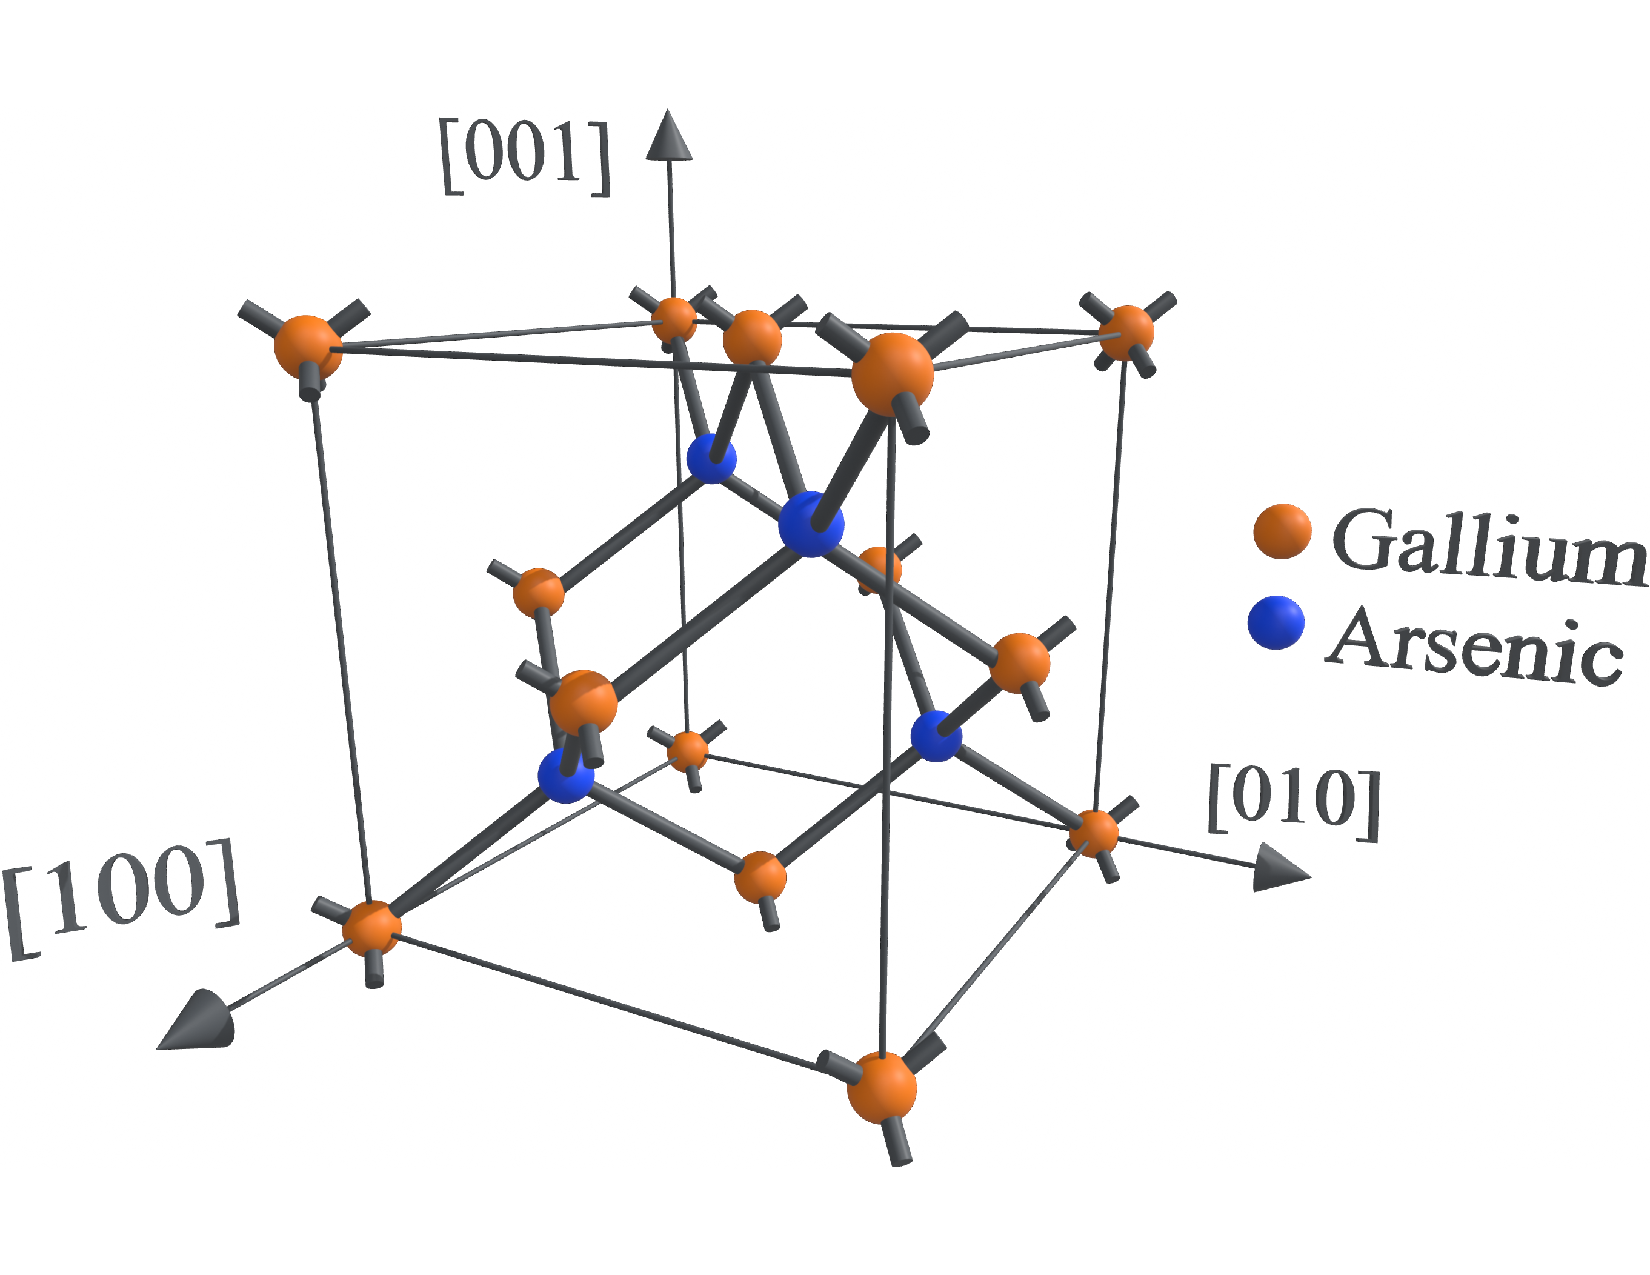
\includegraphics[width=.5\textwidth]{figs/ALGAAS/gaas_unit_cell_mi.pdf}
\caption{The unit cell of gallium arsenide (GaAs) with associated miller indices as coordinate axes}
\end{center}
\label{fig:gaas_uc}
\end{figure}

%% Mention the difference in lattice cell constant between $\gaas$ and $\algaas$?

\subsection{Induced anisotropy in zincblende crystals}
Zincblende structures, like the crystalline materials in question can exhibit birefringent properties when under influence of mechanical stresses and static / low-frequency electric fields ($E_\mathrm{STLF}$); characterized by photoelastic and electro-optic effects respectively. 

\subsubsection{The (linear) electro-optic (Pockel's) effect}

For non-centrosymmetric crystalline media there exists a non-zero rank 2, $6 \times 3$ tensor ($r_{ij}$) connecting a low-frequency \footnote{``low frequency'' meaning orders of magnitude smaller than an optical field it effects} electric field $\vec{E}(f) = [E_x(f), E_y(f), E_z(f)]$ directly to the \hyperref[sec:indicatrix]{indicatrix} ~\cite{yariv,nye}:
\begin{equation}
  \left[ {\begin{array}{c}
   \big( \frac{1}{\Delta n ^2 } \big)_1 \\
   \big( \frac{1}{\Delta n ^2 } \big)_2 \\
   \big( \frac{1}{\Delta n ^2 } \big)_3 \\
   \big( \frac{1}{\Delta n ^2 } \big)_4 \\
   \big( \frac{1}{\Delta n ^2 } \big)_5 \\
   \big( \frac{1}{\Delta n ^2 } \big)_6 \\
  \end{array} } \right]
  =
%
 \left[ {\begin{array}{ccc}
   r_{11} & r_{12} & r_{13}\\
   r_{21} & r_{22} & r_{23}\\
   r_{31} & r_{32} & r_{33}\\
   r_{41} & r_{42} & r_{43}\\
   r_{51} & r_{52} & r_{53}\\
   r_{61} & r_{62} & r_{63}\\
  \end{array}} \right]
 %
 \left[{\begin{array}{c}
   E_x (f)\\
   E_y (f)\\
   E_z (f)\\
 \end{array}} \right]
\end{equation}

\noindent The $i$ index runs over the terms in the indicatix equation:
\begin{equation}
\bigg(\frac{1}{\Delta n_x^2} \bigg) x^2\ + \bigg(\frac{1}{\Delta n_y^2} \bigg) y^2 + \bigg(\frac{1}{\Delta n_z^2} \bigg) z^2 + 2 \bigg(\frac{1}{\Delta n_{xz}} \bigg)xz + 2 \bigg(\frac{1}{\Delta n_{yz}} \bigg)yz + 2 \bigg(\frac{1}{\Delta n_{xy}} \bigg)xy = 1
\end{equation}

%%Detail on some prior knowledge of $f \leq f_\mathrm{max}$? (Pockels cell specs?)

\subsubsection{$r_{ij}$ for zincblende crystals ($r_{\bar{4}3m, ij}$)}

The form of the electro-optic tensor for zincblende crystals (including $\gaas$ and $\algaas$) reduces such that $r_{ij} = r_{41} = r_{52} = r_{62} \neq 0$ with all other terms being zero:

\begin{equation}
r_{\bar{4}3m,ij} =
 \left[ {\begin{array}{ccc}
  0 & 0 & 0\\
  0 & 0 & 0\\
  0 & 0 & 0\\
  r_{41} & 0 & 0\\
  0 & r_{52} & 0\\
  0 & 0 & r_{63}\\
 \end{array}} \right]
\end{equation}

\noindent Where also $r_{41} = r_{52} = r_{63}$

\subsubsection{New principal (electro-optic) dielectric axis for zincblende structures}

In general the principle dielectric axes of the new ellipsoid do \textbf{not} coincide with the axes of the ellipsoid of the unperturbed crystal. The form of the index ellipsoid for a zincblende crystalline material accounting for the electro-optic tensor and some generalized DC electric field $\vec{E}$ expressed in terms of the crystallographic axes is given by:
\begin{equation}\label{eq:zindicatrix}
\bigg(\frac{1}{n_o^2} \bigg) x^2\ + \bigg(\frac{1}{n_o^2} \bigg) y^2 + \bigg(\frac{1}{n_o^2} \bigg) z^2  + 2r_{41} E_{[100]} yz + 2r_{41} E_{[010]} xz + 2r_{41}E_{[001]} xy= 1
\end{equation}

\noindent Where we have set $n_x = n_y = n_z = n_o$ for zincblende structures.

\noindent Eigenvectors of the above tensor equation, produce the two principal axes:	

\begin{equation}
 \left[ {\begin{array}{ccc}
   \big( \frac{1}{n_o ^2} \big)& r_{41}E_{[001]} & r_{41} E_{[010]}\\
   r_{41}E_{[001]} & \big( \frac{1}{n_o ^2} \big) &  E_{[100]}\\
   r_{41} E_{[010]} & r_{41} E_{[100]} & \big( \frac{1}{n_o ^2} \big)\\
  \end{array}} \right]
\end{equation}

\subsubsection{The photoelastic effect}

General stresses and strains, when applied to a material, also impact the indicatrix and demonstrated with the 4th-rank photoelastic tensor $p_{i j \alpha \beta}$:

\begin{equation}
 \bigg( \frac{1}{\Delta n^2} \bigg)_{ij} = p_{ij\alpha \beta} \epsilon_{\alpha \beta}
\end{equation}

where

\begin{equation}\label{eq:indicgen_stress2strain}
	\epsilon_{\alpha \beta} = r_{\gamma \alpha \beta}E_{\alpha} + s_{\alpha \beta \gamma \theta } \sigma_{\gamma \theta}
\end{equation}

Where $\alpha$ and $\beta$ are dummy indices connecting the elasto-optic ($p_{ij \alpha \beta}$) tensor to the stress tensor ($\epsilon_{\alpha \beta}$) via stress-strain / piezoelectric relations:

\begin{equation}\label{eq:indicgen_elasto_optical}
 \begin{split}
	p_{ij \alpha \beta} = \pi_{ij \gamma \theta} C_{\gamma \theta \alpha \beta}
	\\
	\pi_{ij\gamma \theta } = p_{ij \alpha \beta} s_{\alpha \beta \gamma \theta}
 \end{split}
\end{equation}

For realistic mirror coatings, heteroepitaxial bonding between $\gaas$/$\algaas$ layers may produce an intrinsic strain within the HR stack and can lead to the existence of a static non-negligible birefringence throughout the coating layers \cite{Cole:16}.

\subsubsection{The generalized indicatrix}
Both forms of the induced birefringence (electro-optic and photo-elastic) can be incorportated into a condensed form \cite{nye}:

\begin{equation}\label{eq:indicgen}
	\bigg( \frac{1}{\Delta n^2} \bigg)_{ij} = r_{ijk}E_k + p_{ij \alpha \beta} \epsilon_{\alpha \beta}
\end{equation}


%%New principal dielectric axes for zincblende structures (zinblende photoelastic tensor, zincblende electro-optic tensor)

\subsection{EO Modulation}\label{sec:EOM}
Imparting phase modulations onto an optical carrier field is a common application of the electro-optic effect. Electro-optic modulators (EOMs) or Pockel cells are sold as a standard optical components usually composed of a monolithic crystalline material sandwiched between two capacitor plates connected to a single electrical input port (typically coaxial) designed to take in a voltage input of frequency ($\Omega$) within a specified modulation amplitude and frequency bandwidth. When the field amplitude across the crystal is driven by a voltage controlled oscillation, the coefficients within the electro-optic tensor vary linearly. The voltage amplitude of the signal input is proportional to the strength of the phase modulation on the optical carrier field of frequency ($\omega$) and is commonly quantified in terms of a modulation index ($\beta$).

%%Consider a specific crystal that gives us our $\beta \mathrm{sin}(\Omega t)$

\begin{equation}\label{eq:inp_EOM}
E_\mathrm{out} = E_o e^{i \omega t + \beta \mathrm{sin}( \Omega t)} \approx
\end{equation}

\begin{figure}[!ht]
\begin{center}
	\begin{subcaptiongroup}
	     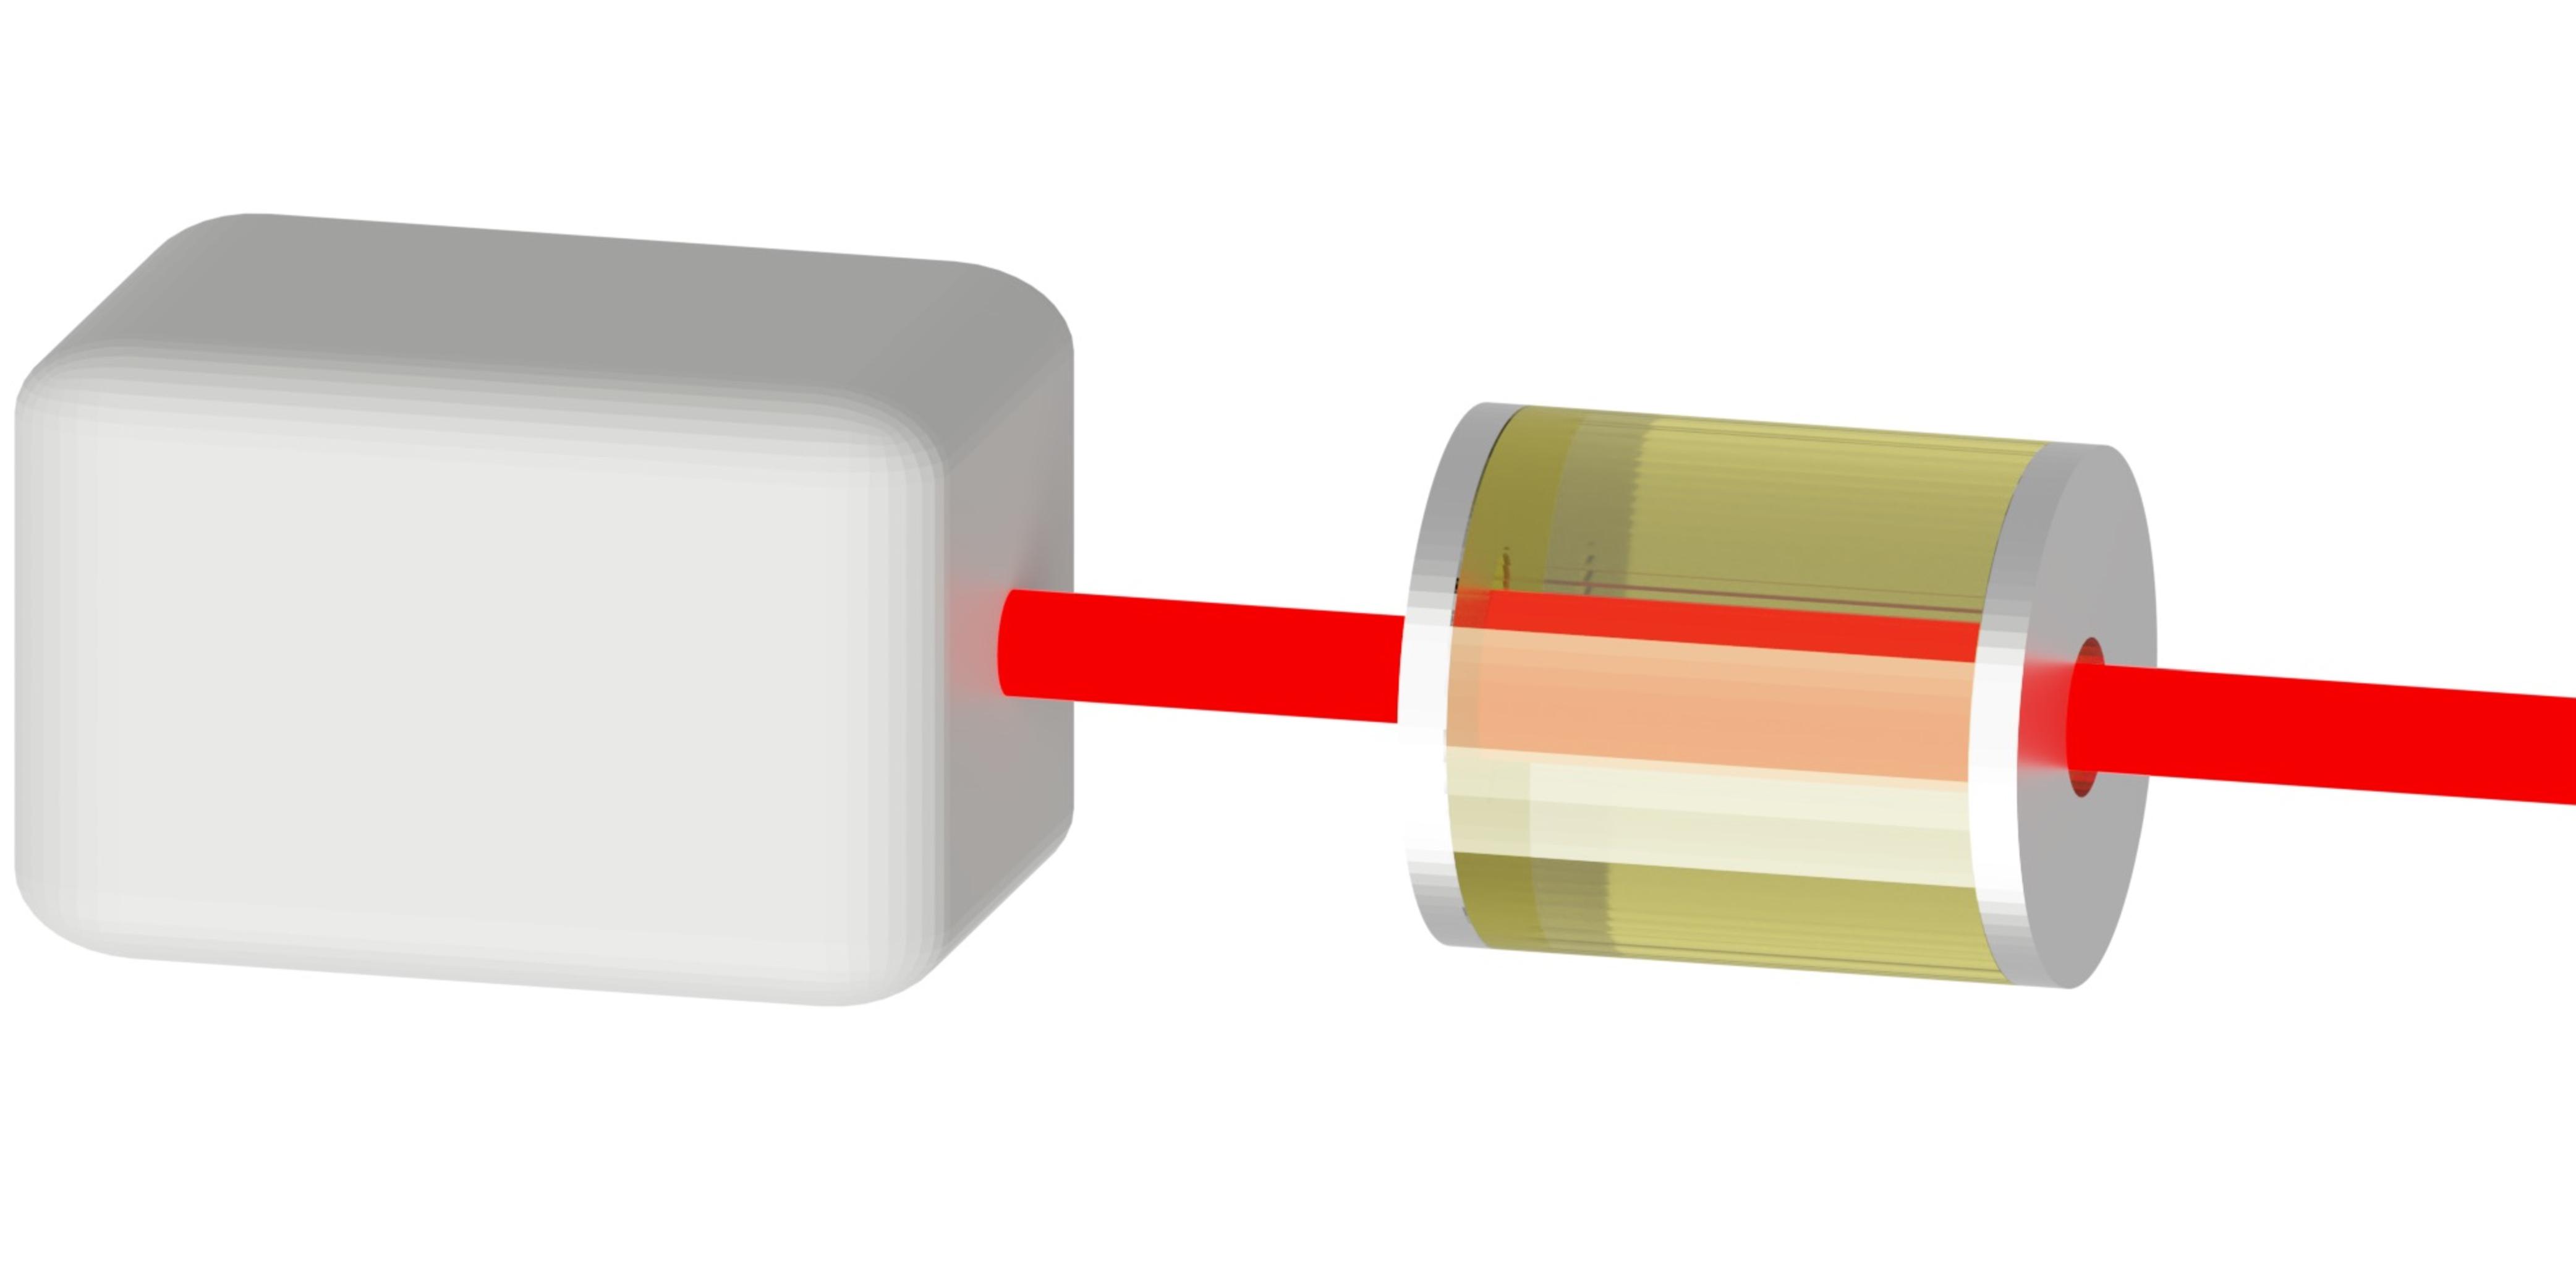
\includegraphics[width=.6\textwidth]{figs/ALGAAS/eom_l_assembly.pdf}
	     \phantomcaption\label{pc_longitudinal}
	     \\
	     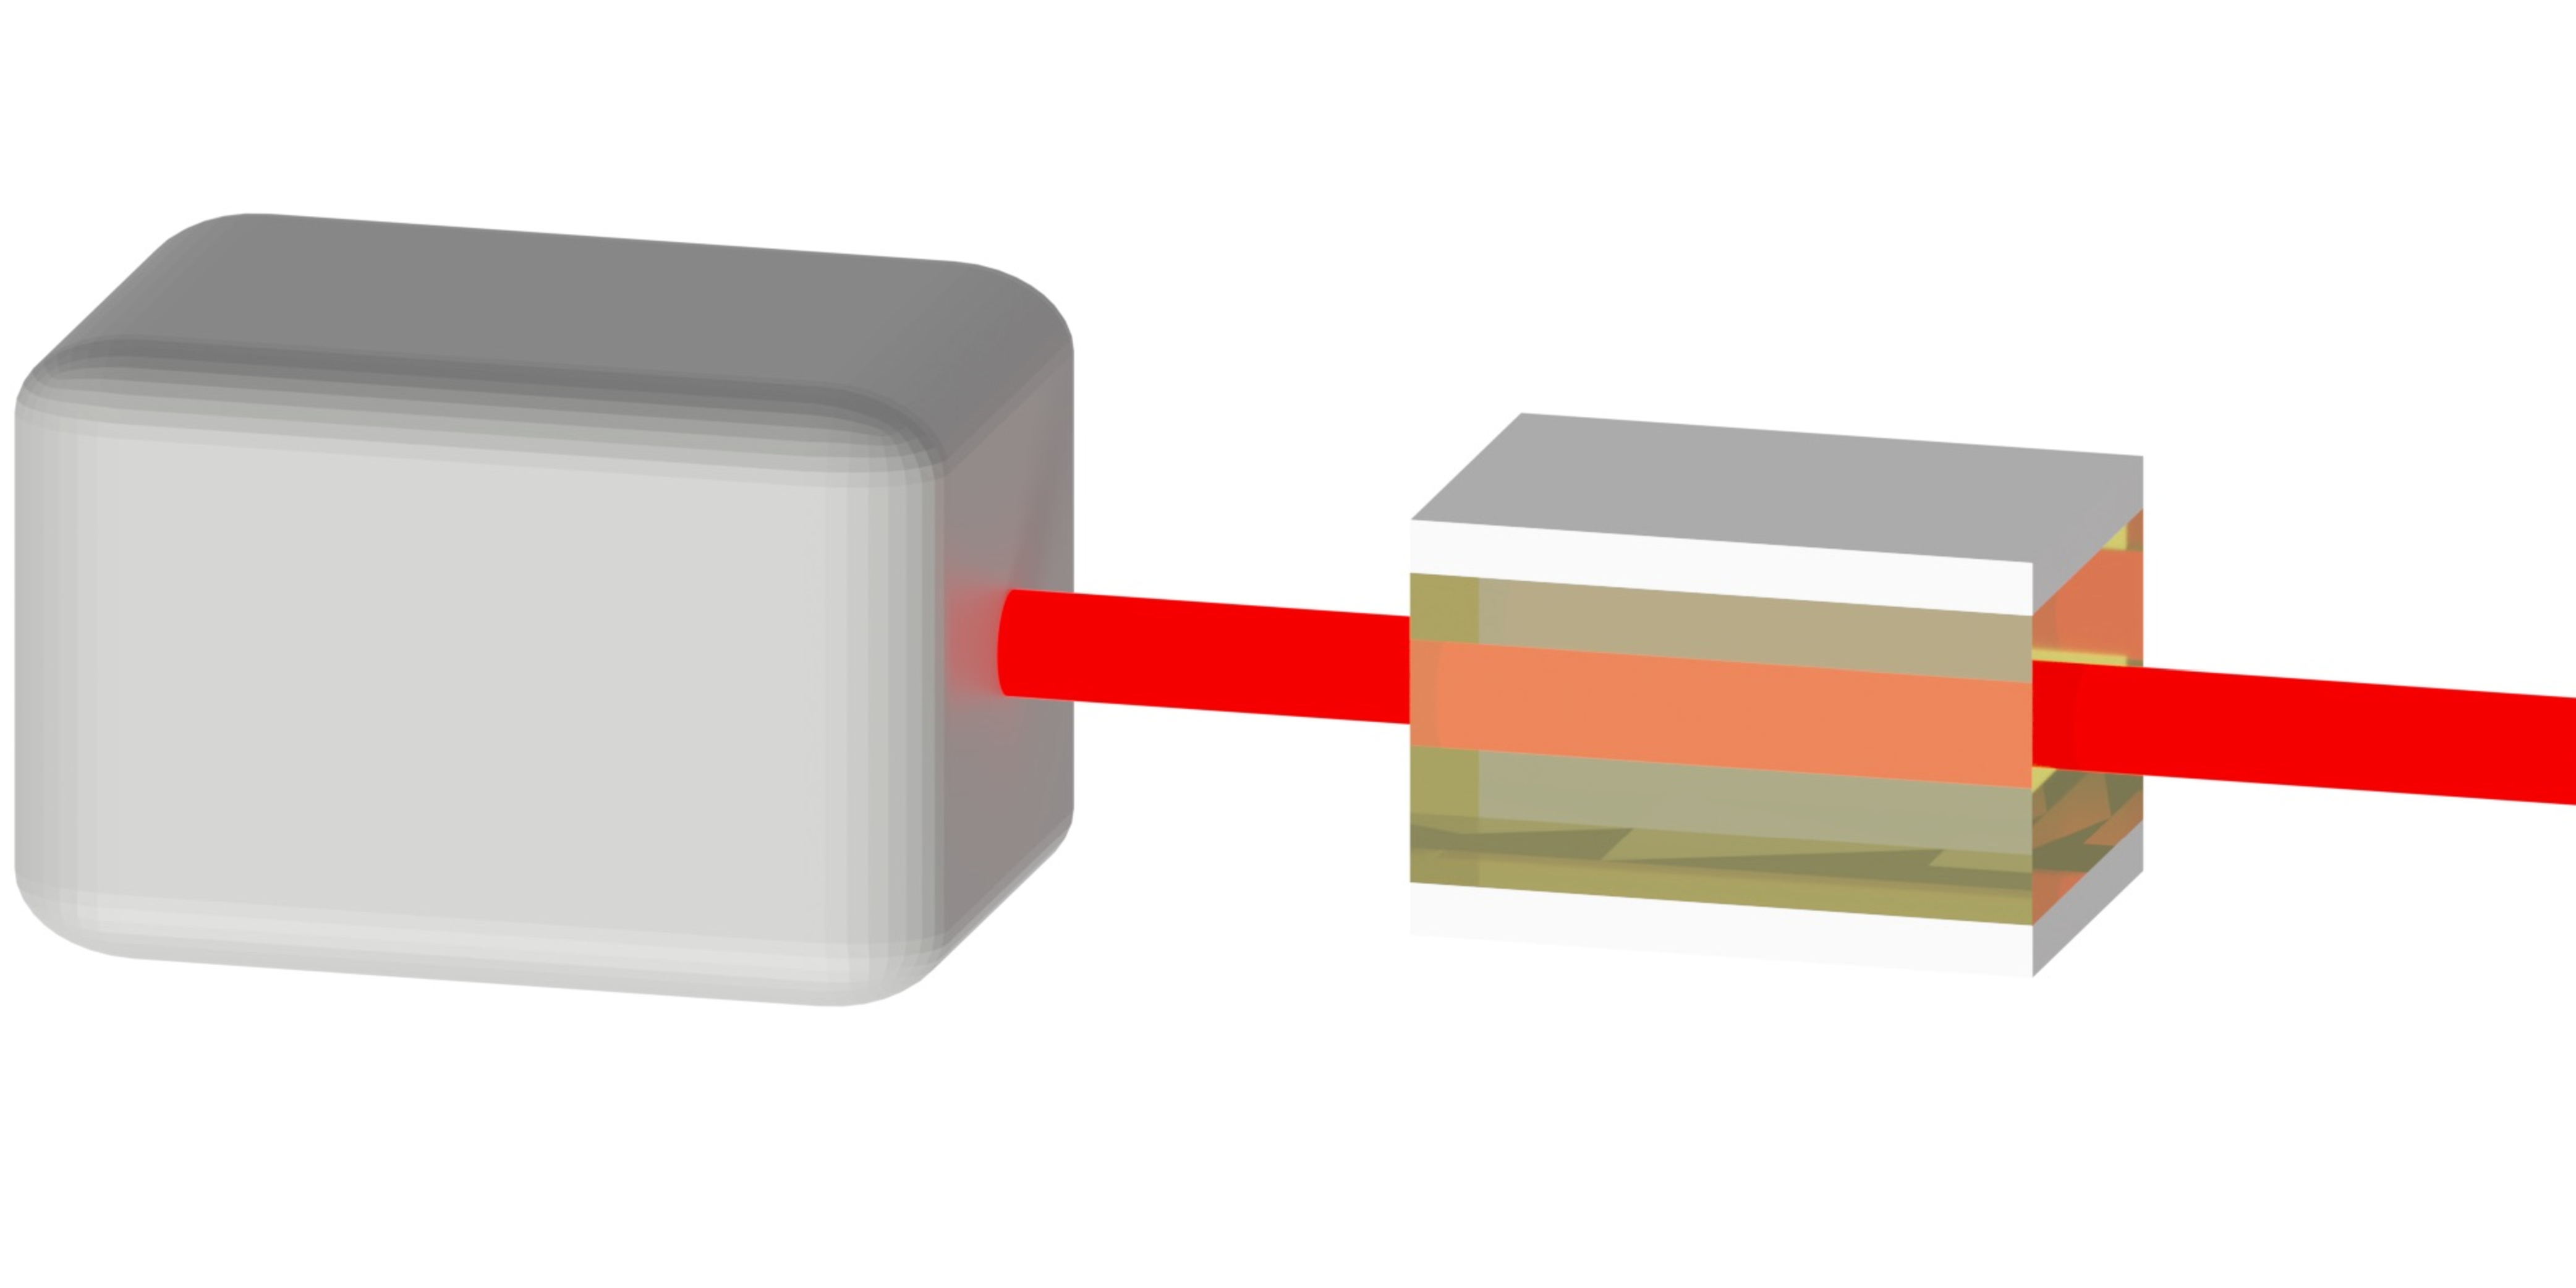
\includegraphics[width=.6\textwidth]{figs/ALGAAS/eom_t_assembly.pdf}
	     \phantomcaption\label{pc_transverse}
	\end{subcaptiongroup}
\end{center}
    \caption{Longitudinal and Transverse Pockels cells}
    \label{fig:lpc_and_tpc}
\end{figure} 


Bessel function approximations sufficiently demonstrate that the phase modulated carrier field imparts power to optical sideband fields separated in frequncy by an integer multiple of the modulation $n \cdot \Omega$. Typically $\Omega$ is a chosen frequency used for optical heterodyne detection; while for noise-driven modulation, the phase coupling shows strong coorelation to the relevant E-field spectra alongside the length of the beam propogation within the electro-optic media.

\subsection{Optical anisotropy of a HR $\gaas$ / $\algaas$ stack}
A comprehensive review of the relevant birefringent properties of a HR $\gaas$/$\algaas$ mirrorstack is due, and for this body of work includes: 1) crystal coordinate considerations when asserting an optical axis on a highly reflective crystalline stack manufactured by the Thorlabs crystalline coatings division, 2) citations of coating parameters and observed intrinsic birefringence from the highly reflective coating stack in question, 3) analysis of the differential electro-optic effect on the phase of a reflected beam, and 4) estimating the the differential phase noise in LIGO based on preliminary electric field measurements measured at LHO.

\begin{figure}[!ht]
    \begin{subcaptiongroup}
	    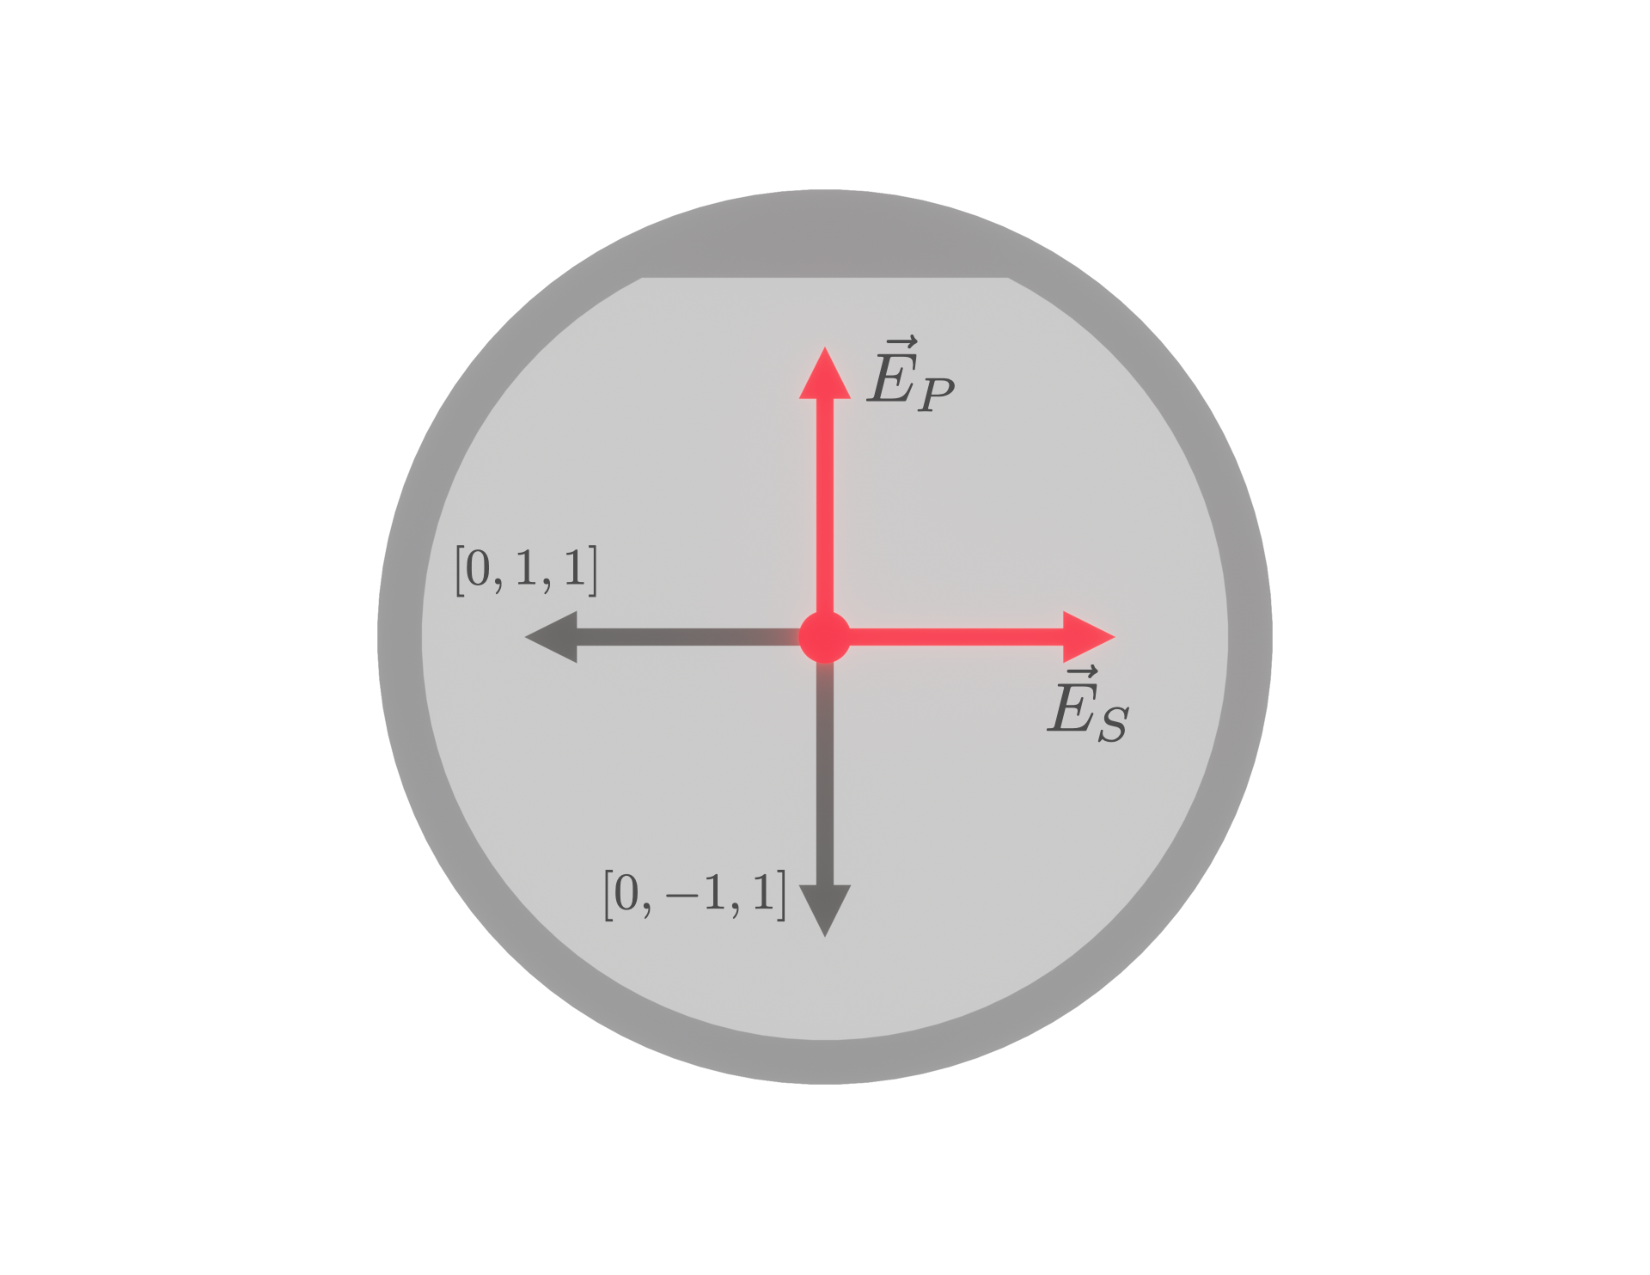
\includegraphics[width=.5\textwidth]{figs/ALGAAS/coating_orientation_normal.pdf}
	    \phantomcaption\label{co_normal}
	    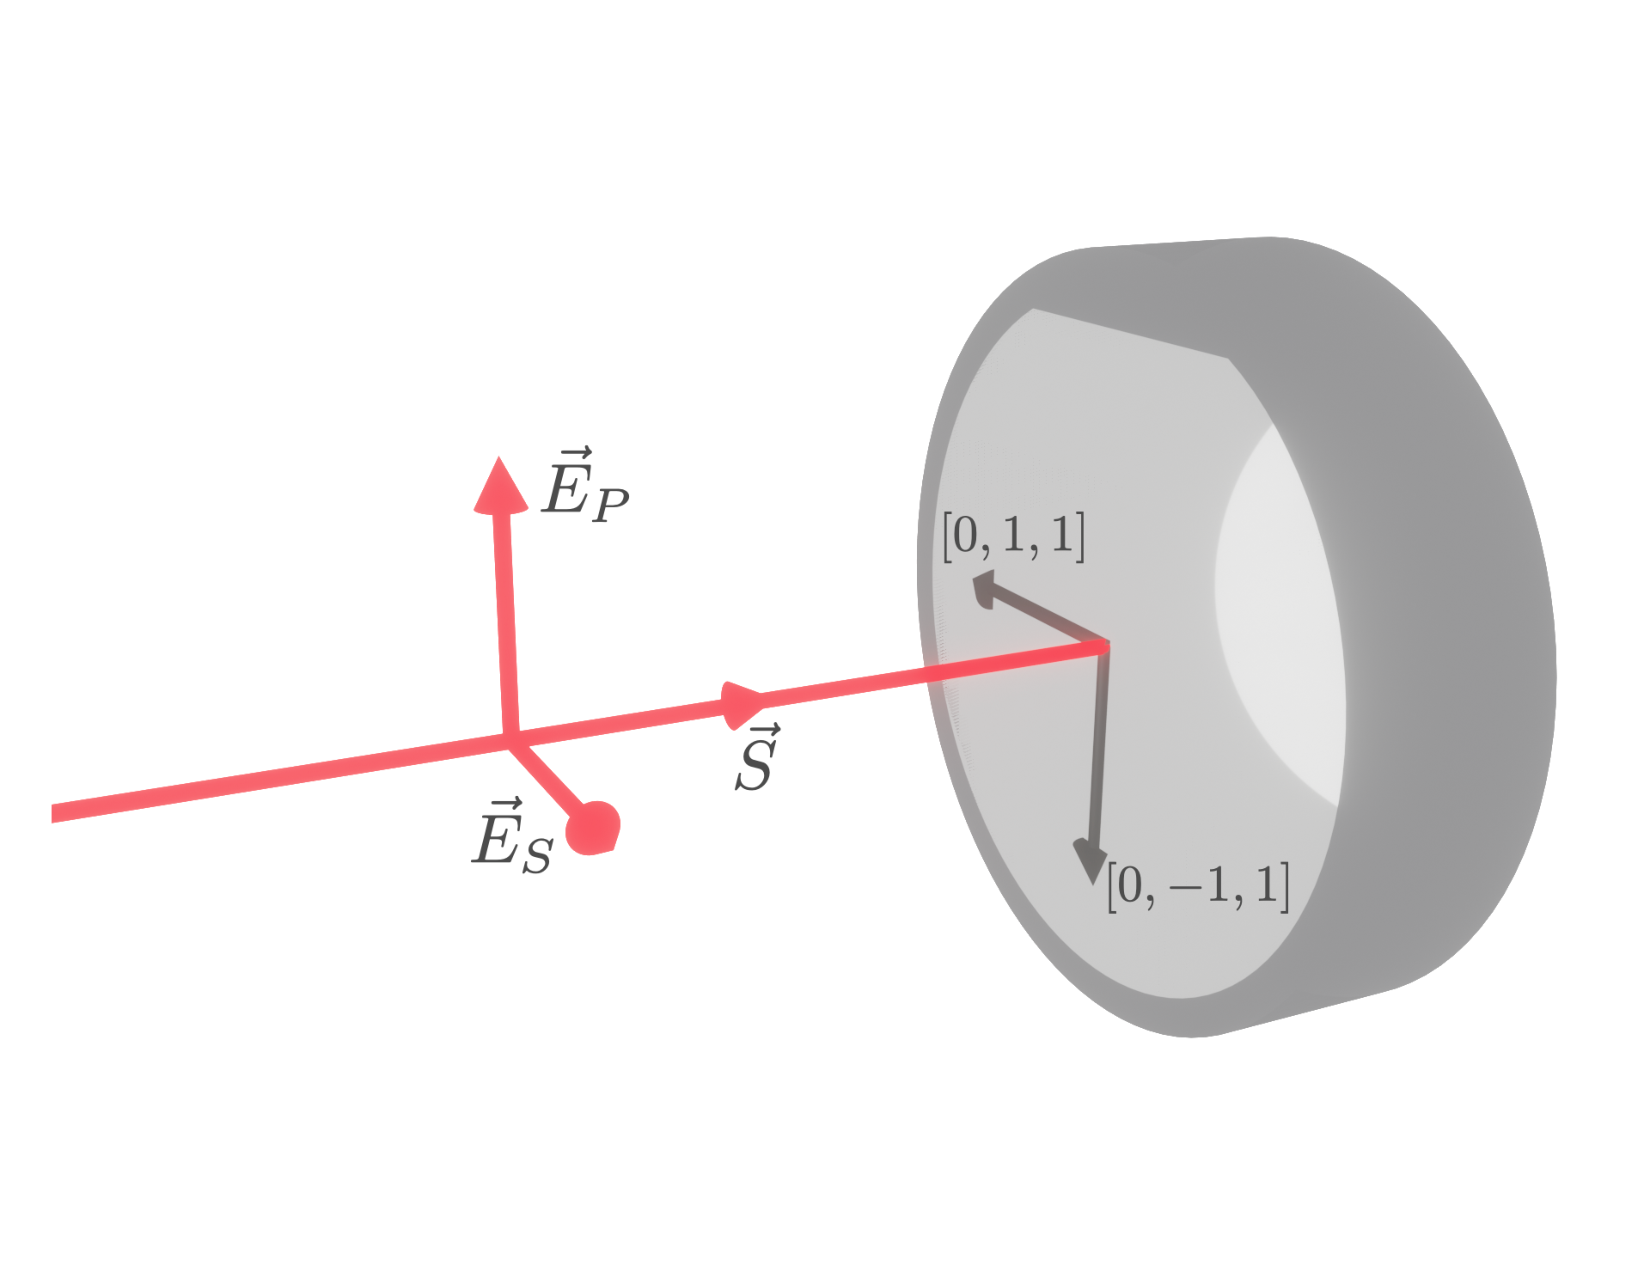
\includegraphics[width=.5\textwidth]{figs/ALGAAS/coating_orientation_isometric.pdf}
	    \phantomcaption\label{co_iso}
    \end{subcaptiongroup}
\caption{The beam propogation axis ($\vec{S}$, $[-100]$) with respect to the AlGaAs/GaAs crystal axes. The axis formed by the [100] plane normal is drawn parallel with the beam axis (z-axis) and the polarizations of incident and reflected beam oscillate along vectors within the plane formed by the normal of that axis. The AlGaAs coating is grown with a flat indicating a line within the [0-11] plane; where the plane normal points towards the sample center.}
\label{fig:algaas_coords}
\end{figure}

\subsubsection{Miller indices for highly reflective coatings $\gaas$/$\algaas$ coatings}
Up to this point three varieties of orthonormal coordinates are addressed: the crystal axis (as indicated by Miller index plane normals), the principal dielectric axis (based on diagonalization of the indicatrix), and an optical beam axis (when considering a desired (laser) light propogation). The asserted beam axis is cited \ref{fig:algaas_coords}.

\subsubsection{Electro-optic coupling to the reflected phase of a HR mirror coating}
With our chosen beam axis, the influence of an isotropic white noise field ($E_n = [E_{nx},E_{ny},E_{nz}]$) is considered:

\begin{equation}
 \left[ {\begin{array}{ccc}
   \big( \frac{1}{n_o ^2} \big)& r_{41}E_{ny} & r_{41} E_{nx}\\
   r_{41}E_{ny} & \big( \frac{1}{n_o ^2} \big) & r_{41} E_{nz}\\
   r_{41} E_{nx} & r_{41} E_{ny} & \big( \frac{1}{n_o ^2} \big)\\
  \end{array}} \right]
\end{equation}

Assuming $E_n$ is small, the indicatrix change of $E_{nx}$ and $E_{ny}$ relative to $E_{nz}$ (as seen by the beam polarization) will be small ($r_{41}E_{n(x/y)} \ll r_{41}E_{nz}$). After diagonalizing with relevant terms \footnote{Note that the form of the tensor is still in the crystal coordinates but the $E_n$ terms are placed in the tensor such that their directions align with beam axis coordinates.} in the tensor, we are left with the following eigenindices:

\begin{equation}
\begin{aligned}
n_x' & = n_o - r_{41}E_{nz} \\
n_y' & = n_o + r_{41}E_{nz}
\end{aligned}
\end{equation}

%How the modulation of the phase of the carrier field is dependent on the orientation of its wave vector with respect to the crystal structure, the modulating electric field direction and strength, (other items to discuss in terms of introducing the effect)
%% For GaAs @ $10.6\mu$ $r_{41} = 1.6 \times 10^{-12}$ [m/V]
%% Adachi estimate for $\mathrm{Al_{x}Ga_{1-x}As}$?
%% Relevant eigenpolarizations, non-optical field $E_y = E_z = 0$?}
%% FIGURE: SUB1 Transformed indicatrix (Before and after $E_x$)
%% FIGURE: SUB2 Ellipse cross section. New eigenpolarizations and corresponding indices and their influence on incident field (Marty's result)

Assuming we are operating in a coordinate system suggested in \hyperref[fig:algaas_coords]{Figure 3.4}, which plane is impacted by some $E_\mathrm{noise}$? Revisiting the \hyperref[eq:zindicatrix]{indicatrix} we can see that for even non-zero z and y components that the only coupling to the input beam polarization is the index along the cross coupled zy-axis through $E_z$ is that of the $E_x$ term. This gives us the ability to easily diagonalize the indicatrix tensor by setting non-relevant field terms to zero.
Fejer and Bonilla take an analytical approximation approach when finding the impact of the electric field to the change in phase of the light through a crystalline anisotropic thin film ($\lambda/4$) stack \cite{bonillafejer}.

\begin{equation}
\hat{\phi}' = \frac{\pi n_1 z}{1-z^2}(z^{2N} -1) \frac{z^{2N} \frac{(n_f)^2}{n_2 n_3}(n_2 \kappa_{\gamma 2} + n_3\kappa_{\gamma 3}) - (n_2 \kappa_{\gamma 3} + n_3\kappa_{\gamma 3})}{(n_1)^2 -(n_f)^2 z^{4N}}
\end{equation}

with $z = \frac{n_2}{n_3}$
and
$
\kappa_{\gamma j} = \frac{d}{d \gamma} \mathrm{log}(n_j h_j)|_{\gamma =\gamma_{O}} \bigg(\frac{\hat{n}_j'}{\hat{n}_j} +\frac{\hat{h}_j'}{\hat{h}_j} \bigg)
$

With $\kappa$ being a scalar parameter.
%%FIGURE: Cross sectional view of multilayer coating

\begin{figure}[!ht]
    \begin{subcaptiongroup}
	    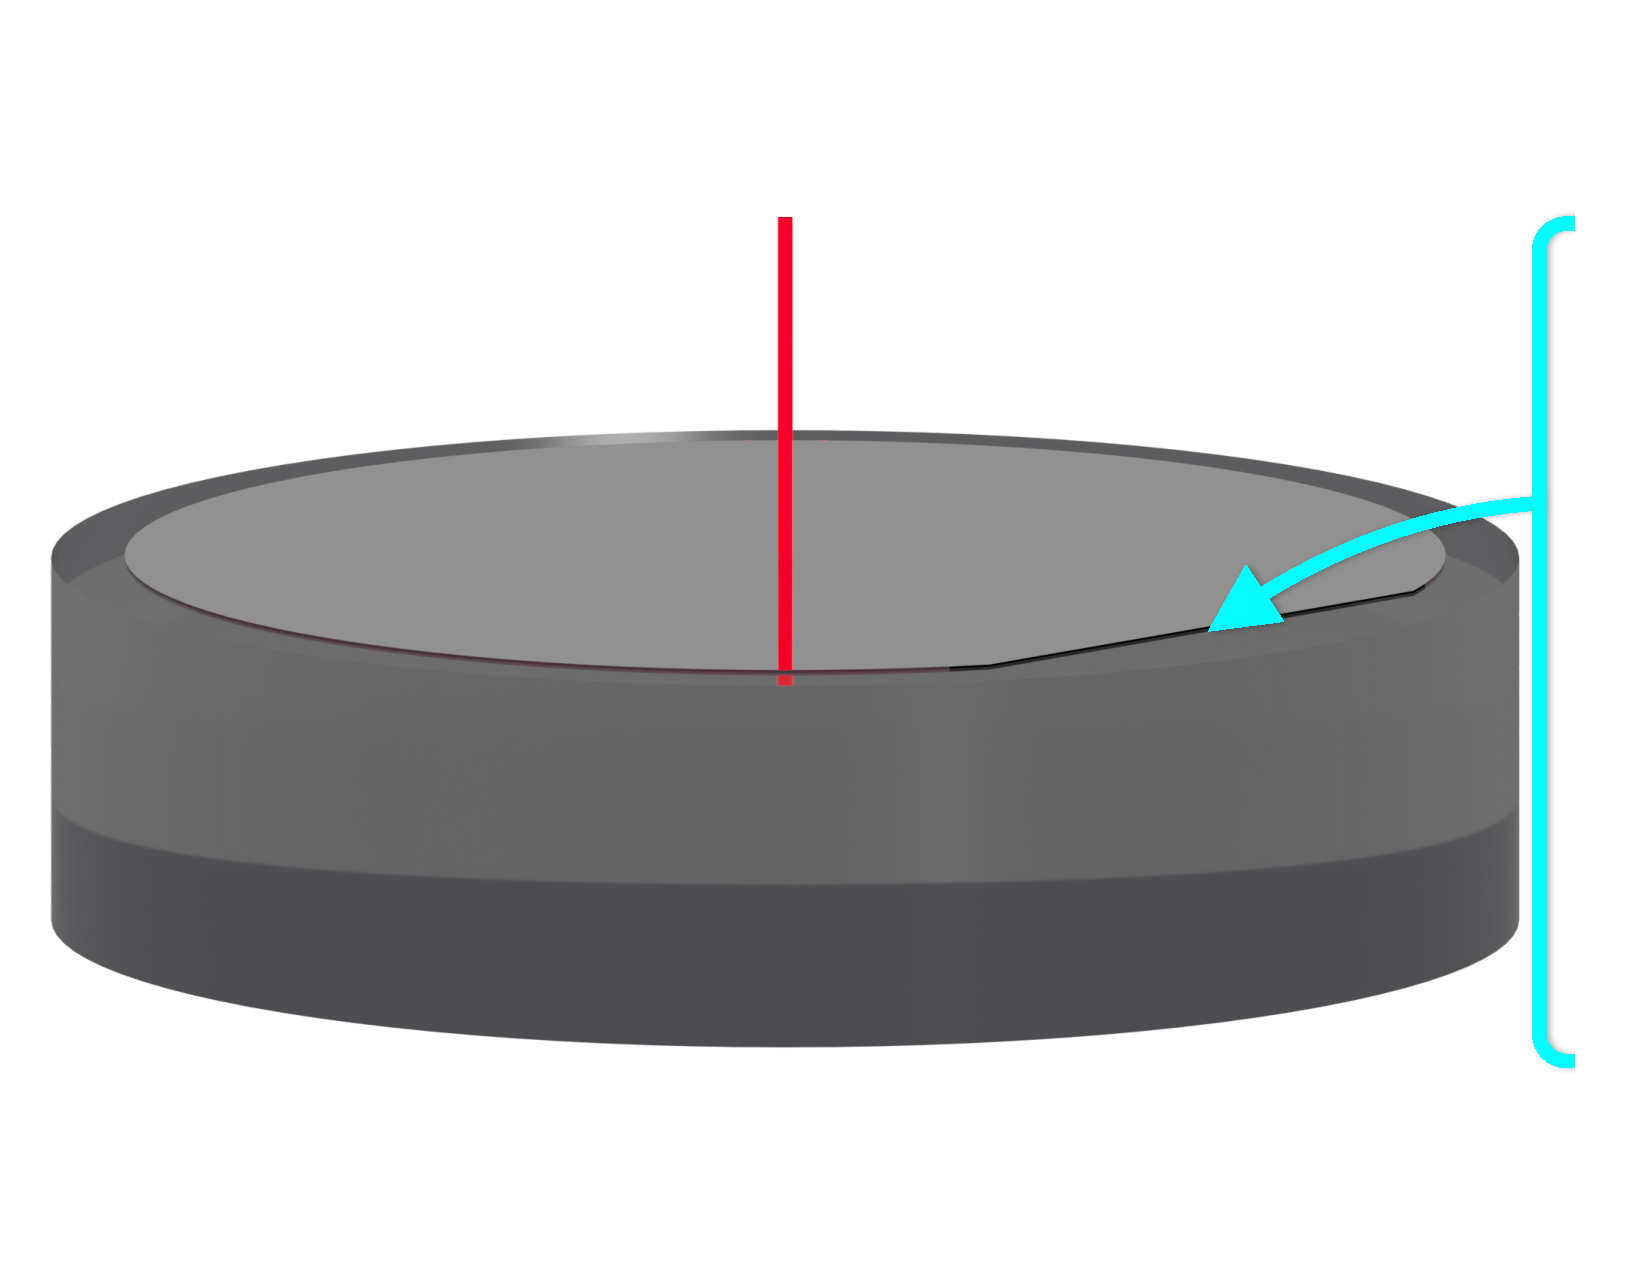
\includegraphics[width=.55\textwidth,page=1]{figs/ALGAAS/ALGAAS_HR_layers_1.pdf}
	    \phantomcaption\label{HRiso}
	    \includegraphics[width=.55\textwidth,page=2]{figs/ALGAAS/ALGAAS_HR_layers_1.pdf}
	    \phantomcaption\label{HRxsection}
    \end{subcaptiongroup}
\caption{The beam propogation axis ($\vec{S}$, $[-100]$) with respect to the AlGaAs/GaAs crystal axes. The axis formed by the [100] plane normal is drawn parallel with the beam axis (z-axis) and the polarizations of incident and reflected beam oscillate along vectors within the plane formed by the normal of that axis. The AlGaAs coating is grown with a flat indicating a line within the [0-11] plane; where the plane normal points towards the sample center.}
\label{fig:HRlayers}
\end{figure}


\subsubsection{Numerical estimate}

In the appendix of \cite{ballmer2015} Ballmer constructs a coating layer transfer function for a given coating layer k with index $n_k$, and thickness $d_k$, defining right and left propogating modes $\Psi^{R,L}$ repsectively:

\begin{equation}
  \left[ {\begin{array}{c}
   \Psi^\mathrm{R} \\
   \Psi^\mathrm{L} \\
  \end{array} } \right]_{k+1}
  =
%
Q_k D_k
%
 \left[{\begin{array}{c}
   \Psi^\mathrm{R} \\
   \Psi^\mathrm{L} \\
 \end{array}} \right]
\end{equation}

\noindent $D_k$ applies the phase ($\phi_k = 4\pi n_k d_k /\lambda_0$) from a given coating layer, and $Q_k$ applies the transfer function between high-low/low-high index layers transition:

\begin{equation}
Q_k = \frac{1}{2n_{k+1}}
\left[ {\begin{array}{cc}
  n_{k+1} + n_k & n_{k+1} - n_k\\
 n_{k+1} - n_k & n_{k+1} + n_k\\
\end{array} } \right]
\end{equation}

\begin{equation}
D_k =
\left[ {\begin{array}{cc}
  e^{-i \phi_k / 2}& 0\\
 0 & e^{i \phi_k / 2}\\
\end{array} } \right]
\end{equation}
Defining a HR coating stack, the total transfer matrix from vaccum $Q_0$ to the $N$th coating layer is:
\begin{equation}
M = Q_N D_N ...Q_kD_k...Q_1D_1Q_0
\end{equation}
The impact of a differential electric noise field ($E$) on $M$ due to the electro-optic effect on the kth layer, we use the chain rule:

The coating to be studied consists of 36 $\lambda$/4  thick layers of $\gaas$ interspersed with 35 layers of $\lambda$/4 thick $\algaas$. $\gaas$ forms the top and bottom layer to prevent oxygen absorption from the AlGaAs layer. The $\gaas$ layers have an index of $n_{\gaas} = 3.480$ and a thickness of $\Delta d_{\gaas} = 76.43$ nm while the low index $\algaas$ layers are $n_{\algaas} = 2.977$ with thickness $\Delta d_{\algaas} = 89.35$ nm. With the cosntructed matrices, we apply these parameters and compute a differential phase of:

%High Index:  GaAs, n=3.480, layer thickness is 76.43 nm
%Low Index:  $ \mathrm{Al}_{0.92} \mathrm{Ga}_{0.08} \mathrm{As} $, n=2.977, layer thickness is 89.35 nm
%Info from Steve. Written source


\subsection{Measured birefringence from HR $\gaas$/$\algaas$ mirrors}

There are different accounts of a measured birefringence from HR $\gaas$ / $\algaas$ (\href{https://dcc.ligo.org/DocDB/0181/G2200386/001/G2200386.pdf}{Satoshi}, \href{https://nodus.ligo.caltech.edu:8081/CTN/1474}{CTN}, \href{https://dcc.ligo.org/DocDB/0181/G2200559/001/G2200559-v1%20-%20polarization.pdf}{Aidan})

%%Is the measured birefringence static? (Layer bonding method might introduce something?)
%% Does it change from different mounting methods? (Photoelastic) (order of magnitude estimate)
%% Electro-optic ruled out based on field measurements and relative coupling factor.
%% Measurement precision of the coating birefringence? Cavity length, Polarization drifts, etc.

The measured birefringence is estimated to be caused by an intrinsic strain between the epitaxial layers of $\gaas$/$\algaas$. \cite{Cole:2013}

%% Marty's document about Birefringence in Crystalline mirror coatings V.8

\section{Projected DARM coupling (initial)}
To estimate how much DARM coupling can occur, we use use a measured field spectra acquired from installed electric field meters located within LIGO Hanford Observatory ETMX and ETMY vacuum chambers. Taking the upper and the lower EFM measurements in $.3\; [\mathrm{V}/\mathrm{m}/\sqrt{\mathrm{Hz}]}$ @ 60 Hz and $4\times10^{-3}\; [\mathrm{V}/\mathrm{m}/\sqrt{\mathrm{Hz}]}$ @ 4kHz ~\cite{efmlog}.
%% \satoshi{I don't think these values are calibrated. According to Martynov et al. 2016, the fluctuations in the electric filed is $\sim10^{-5}\,\mathrm{[(V/m)/\sqrt{Hz}]}$.}
This along with computed estimate allows us to create an upper limit for what this noise might be assuming incoherent fields between the end stations and a flat frequency response within LIGO's bandwidth.
%%FIGURE: GWINC noise against calibrated electro-optic noise estimate. Full bandwidth

\section{A Short in-air FPC test}
 In seeking a calibrated estimate of the electro-optic effect for the $\gaas$/$\algaas$ mirror coating stack, we sought to measure a driven response of a mirror sample from Thorlab's crystalline mirror coatings division placed within a custom longitudinal Pockels cell mirror mount and monitored with a Pound-Drever-Hall servo. The servo was used to maintain resonance of a circulating Nd:YAG 1064nm carrier beam within an in-air two mirror Fabry-Perot cavity, with the notable mirror coating sample installed within the longitudinal Pockels cell mount and assumed the end mirror position within an in-air two mirror Fabry Perot cavity. As seen in the prior section, the size of the imparted phase noise for currently existing gravitational wave detector configurations is estimated to be small but notable. Investigation through measurement of said effect requires detection methods with sufficient sensitivity for the differential phase noise imparted by the effect. Details and specifications of the detection schema are discussed along with relevant measurements and results. 

%% Driven acoustic modes of the longitudinal pockels cell mirror mounts lead to numerous mounting strategies that will be detailed below. 
\begin{figure}[H]
	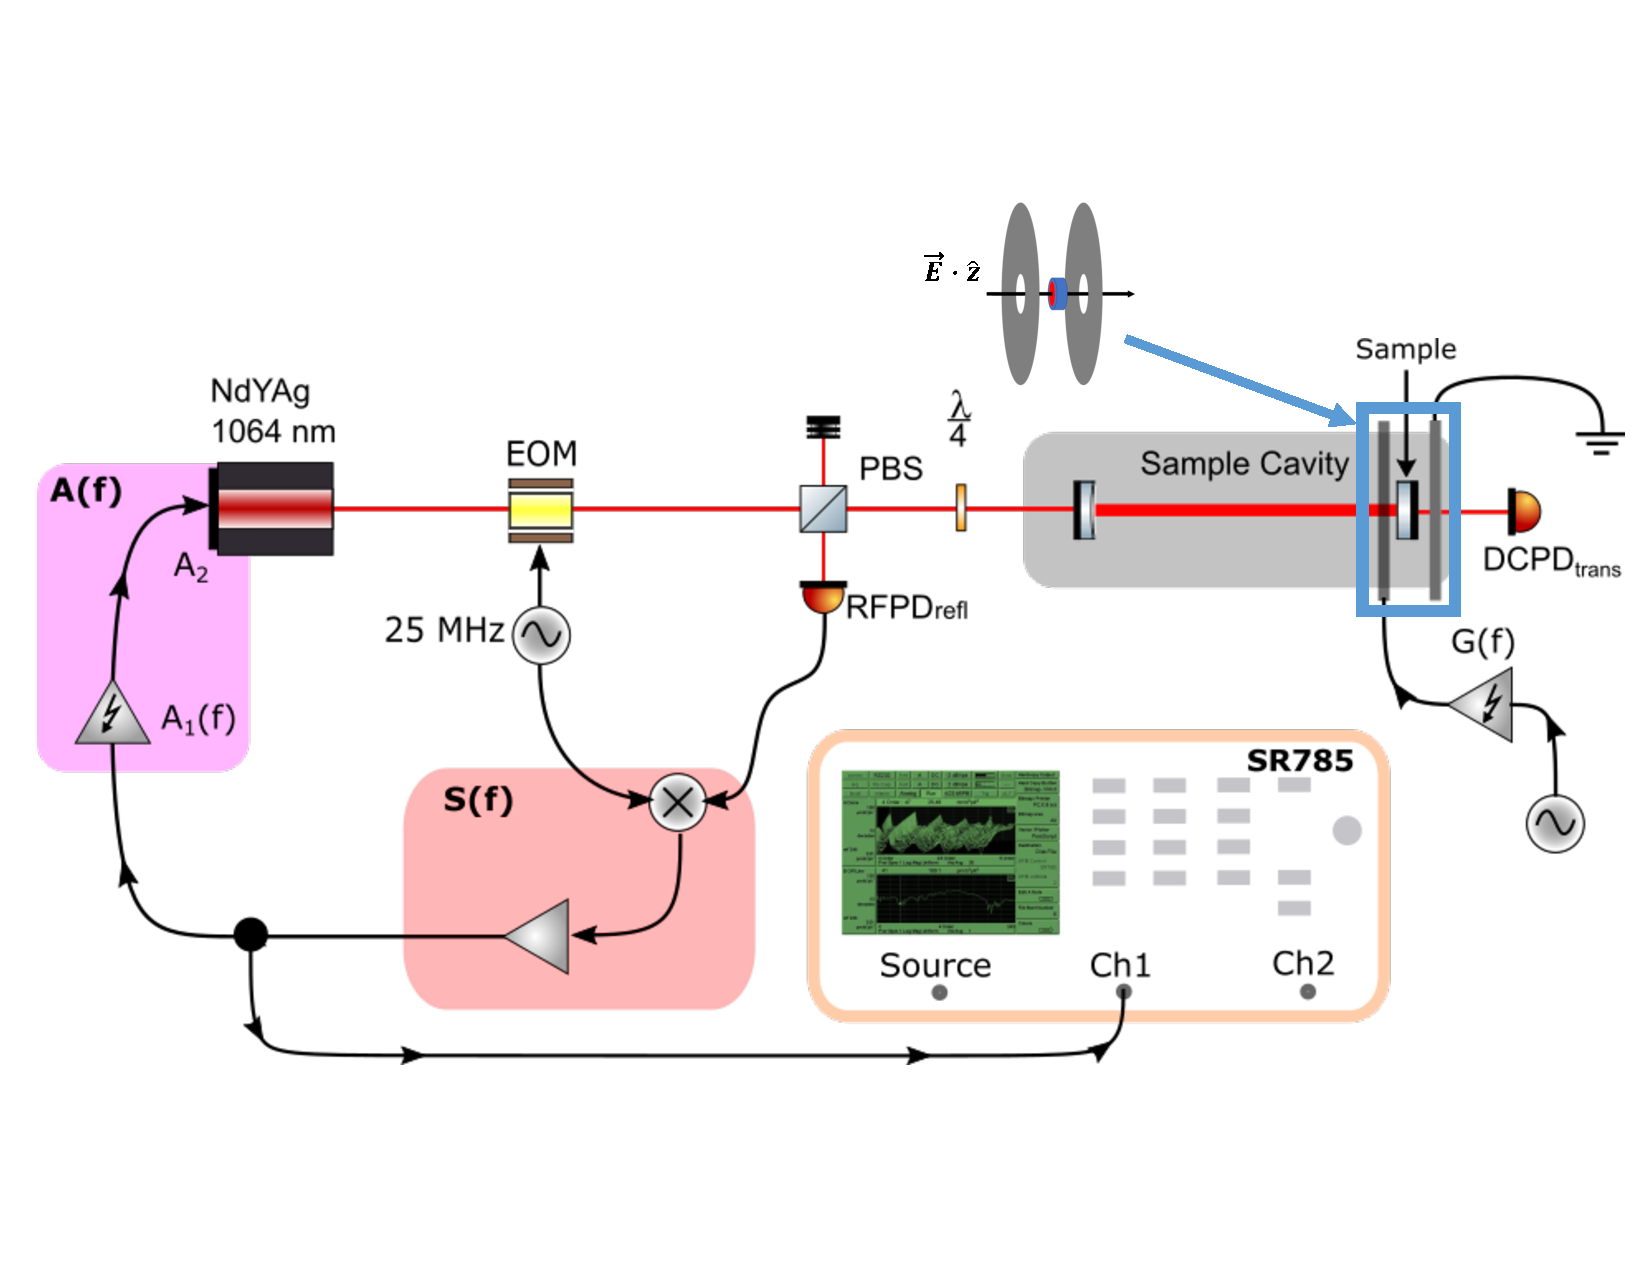
\includegraphics[width=\textwidth]{figs/ALGAAS/algaas_pockels_effect_measurement_schematic.pdf}
	\caption{A simplified and modular schematic of the PDH servo used along with an electrostatic drive mount design comprised of a disk capacitor sandwiching the HR AlGaAs sample, a high voltage amplifier, and a signal / network analyzer.}
\label{fig:simplified_experiment_schema}
\end{figure}
 Measurability of the electro-optic effect is contingent upon two initial design criteria: the sensitivity of the optical plant to be implemented in the PDH servo, and the maximum achievable electric field strength along the beam axis ($|E_z|_\mathrm{max}$).

\subsection{PDH servo}\label{subsubsec:pdh}
The Pound-Drever-Hall technique, originally and commonly used for laser frequency stabilization to an ultra-stable length reference, allows the tracking of the linear phase response of an input carrier field through cavity resonance. The servo fully realizes the ability of an optical cavity to act as a length / frequency discriminator. The alternative cavity offset lock provides a linear response in intensity, which is adequate for some applications but with reduced sensitivity due to the required power reduction by operating off resonance.
The phase measurement is extracted through an optical heterodyne; the co-propogation of a separate (but phase-locked) optical field with a known frequency separation to the carrier reflected from the cavity input. The PDH servo avoids complicated phase-locked two laser configurations, by imposing a phase modulation onto the carrier field via an electro-optic modulator (aka Pockels cell) mentioned in section \ref{sec:EOM}. If the modulation depth given by \ref{eq:inp_EOM} is set such that $\beta < 1$ then the input field may be approximated in terms of the first two Bessel functions $J_0$, $J_1$:

\begin{equation} \label{eq:EOM_trans_field}
E_\mathrm{inp} \approx E_0 [J_0(\beta)e^{i \omega t} + J_1(\beta)e^{i (\omega + \Omega) t} - J_1(\beta)e^{i(\omega -\Omega)t}]
\end{equation}

With a high enough modulation frequency the terms given above can be far enough from the carrier frequency, so that the phase modulation onto the carrier field is mathematically and physically equivalent to imposing separate optical fields (sidebands) which in most cases do not resonate in the optical cavity of interest. Setting a photodiode of area ($A_\mathrm{PD}$) in reflection of the cavity with a coefficient of $r_\mathrm{cav}(\omega,L)$, we measure the reflected power of the input field given by \ref{eq:EOM_trans_field}:

\begin{equation}
 \begin{alignedat}{3}
    &P_\mathrm{refl} && \approx \frac{|E_\mathrm{refl}|^2}{A_\mathrm{PD}} && \\
    & &&\approx \frac{E_0^2}{A_\mathrm{PD}} && \bigg\{J_0^2 |r_\mathrm{cav}(\omega,L)|^2 + J_1^2(\beta)|r_\mathrm{cav}(\omega+\Omega,L)|^2 - J_1^2(\beta)|r_\mathrm{cav}(\omega-\Omega,L)|^2 +  \\
    & && && J_0J_1(\beta)\big[r_\mathrm{cav}\omega,L) r_\mathrm{cav}^*(\omega+\Omega,L)\big] - J_ 0J_1(\beta)\big[r_\mathrm{cav}(\omega,L)r_\mathrm{cav}^*(\omega-\Omega,L)\big]\bigg\}
  \end{alignedat}
\end{equation}

The two trailing terms in the above equation for $P_\mathrm{refl}$ generate a beat frequency term between the carrier and lower and upper sidebands. The magnitude and sign of these beat terms directly relate to the phase of the reflected carrier field and can be measured and transformed to the error signal seen in \ref{fig:pdh_error} using resonant electronics (tuned to a chosen sideband frequency) for amplification and a mixer for demodulation.

\begin{figure}[H]
	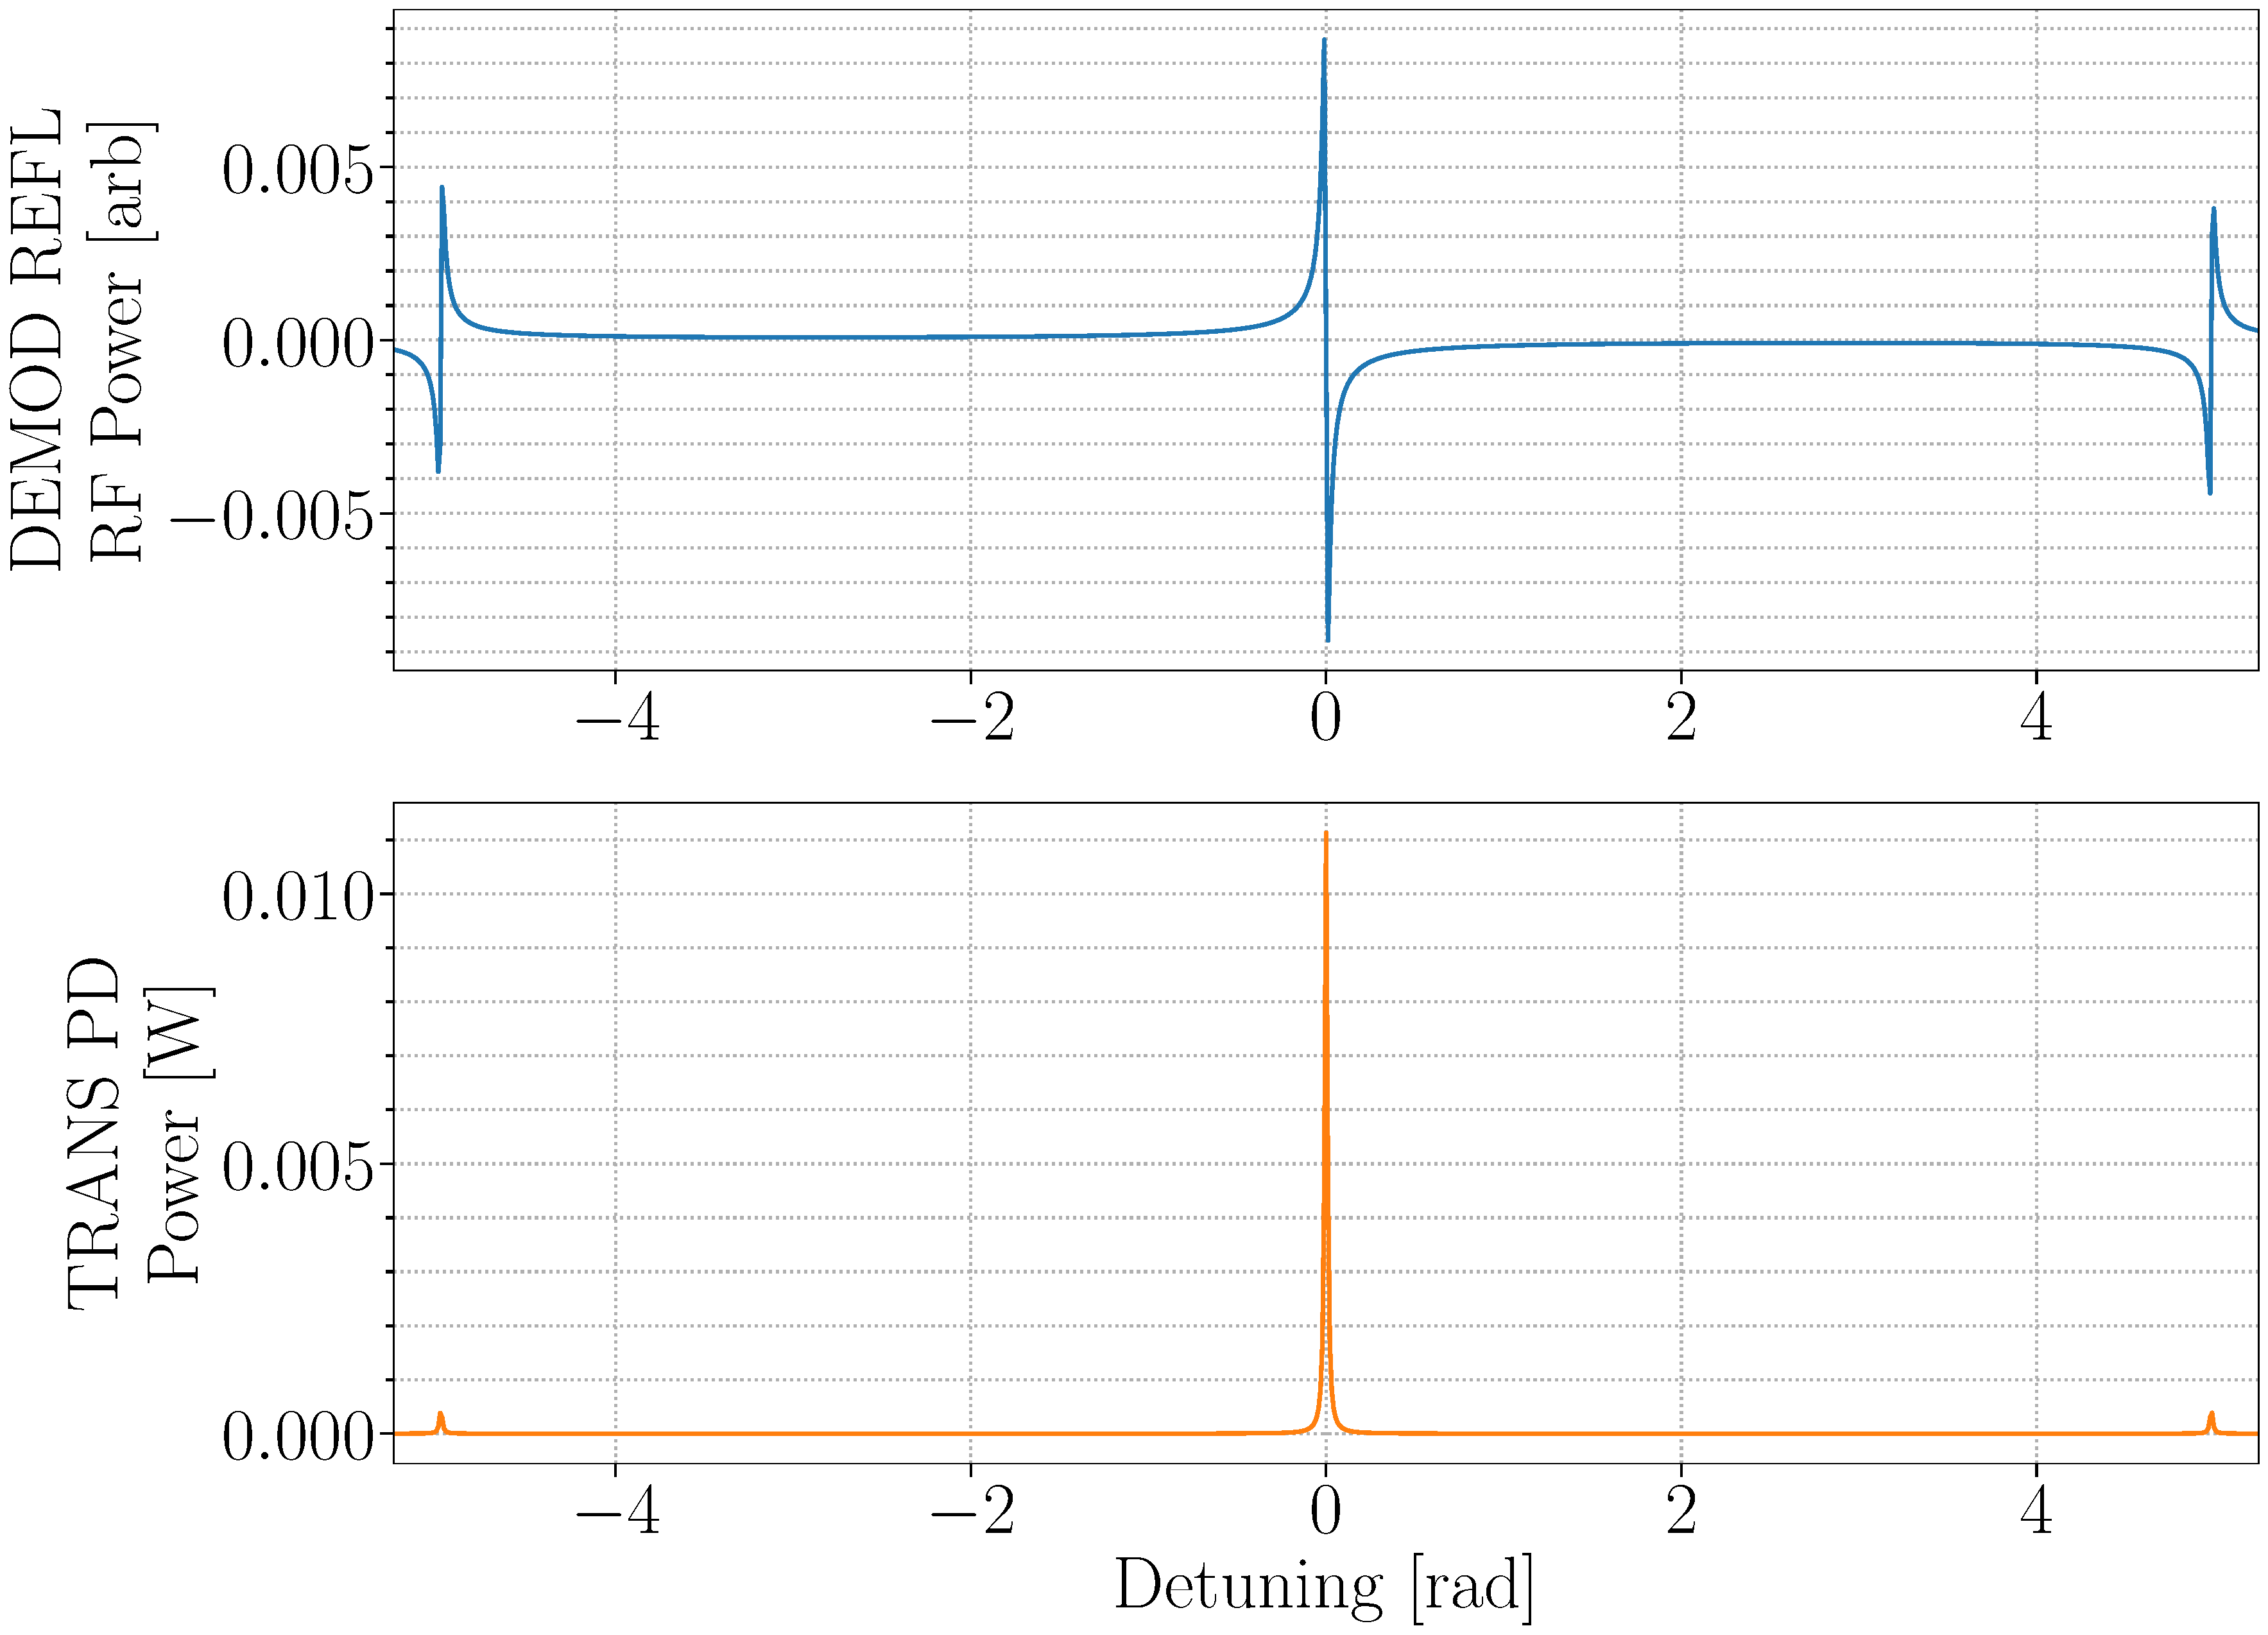
\includegraphics[width=\textwidth]{figs/ALGAAS/pdh_error.pdf}
	\caption{By imposing 25 MHz RF sidebands we have introduced a constant reflected reference field near carrier resonance which when beat with the carrier offers a linear response after demodulating the sideband power. With the introduction of high and low frequency sideband fields, their presence is also detected through the DCPDs and PDH error signal. Their separations from carrier resonance are equal in phase (length, and frequency).}
\label{fig:pdh_error}
\end{figure}

With this linearity and sensitivity at cavity resonance, implementation into PID feedback is the next task as any small detuning of the cavity can be registered as a drift from the loop's zero point and fed back to an actuator with an estimated calibration gain factor. When implemented into a low-noise design, this servo can also be used for a high sensitivity lock-in measurement; and with well characterized instrumentation, calibration of the induced differential phase of the light within the stable reference cavity into differential length (or frequency).


\subsection{Servo Parameters}
The quantity we are attempting to measure is on the order of a length change of ? m/(V/m), motivating a short cavity design as the relative differential length (phase) change scales with the sensitivity $\Delta f / f = \Delta L / L$. Considerations of the lab mirror inventory and mode matching critera lead us to two candidate plano-concave (ROC = 0.333m) HR IBS coated sample input couplers; one from CVI Melles-Griot and another from ATFilms. When paired with the plano-plano GaAs/$\mathrm{Al_{.92}Ga_{.08}As}$  mirror from the Crystalline Mirror Solutions (CMS) division of Thorlabs we create a 0.1665 m long cavity.


\begin{figure}[H]
\begin{center}
\includegraphics[width=.80\textwidth]{ALGAAS/opt_layout_b.pdf}
\end{center}
\caption{\textcolor{red}{Final figure still pending} Detailed optical schema of the experiment. Components highlighted in magenta indicate laser back-reflection protection and output power control. All optics highlighted in PURPLE indicate their function as alignment and mode matching for locking to a triangular ALIGO PMC \textbf{Multiple citations (DCC doc / Fabian's experiment / Erik's experiment)}. Optics highlighted in YELLOW indicate function for alignment and mode matching to the experimental cavity utilizing the HR $\gaas$/$\algaas$ coated mirror sample. Beam profiling to the sample cavity is indicated. For the sake of the numerous mounting strategies tried, the longitudinal pockels cell mirror mount is kept general with the pictured mirror between two disk capacitors}
\label{fig:detailed_optical_layout}
\end{figure}
%%FIGURE: Servo diagram
%%CAPTION: A simplified diagram of the servo used. The highlighted regions of the schematic are intended to provide a modular view; highlighting the components required for the PDH servo to operate.}
The implemented servo design uses a light source from a Mephisto 2000 NE Nd:YAG (1064nm) laser with a 25 MHz phase modulation from a New Focus Model 4003 IR resonant phase modulator. As indicated in the figure above, the electronics chain can be decomposed into various filter components: $S(f)$, $A(f)$, and $A_\mathrm{thermal}(f)$

\subsubsection{Sensing S(f)}
The sensing filter electronics are composed of a single element photodiode (from?) with a QE of ? and the response found in appendix ?. The signal is then mixed with a 25 MHz oscillator phased 180 degrees ? m of cable so the measured beat signal while sweeping through resonance generates the \hyperref[fig:pdh_error]{PDH error signal profile}.
\begin{itemize}
\item 25 MHz RFPD
\begin{itemize}
\item Transimpedance measurement (necessary? or should I just use the mixer out PDH to summarize PD/mixer response)
\end{itemize}
\item Frequency Stabilization servo (modified MIT FSS (DCCD980536)) (LTspice model in appendix)
\end{itemize}


\subsubsection{Actuation A(f)}
\begin{itemize}
\item Mephisto 2220 PZT response (capacitance estimated from HVA drive measurement with and without connection to PZT)
\item Channel 3 of SVR 350-3 BIP High Voltage Amplifier from Piezomechanik GmbH with Pomona box (elog 412)
%%FIGURE: Frequency response of A(f)}

\end{itemize}

\subsubsection{Low frequency servo (Thermal loop)}
\begin{itemize}
\item Passed signal from FSS $\rightarrow$ integrators $\rightarrow$ Laser thermal actuator input
\end{itemize}

\subsubsection{OLG(f)}
Isn't quite $\mathrm{A}(f)*\mathrm{S}(f)$ as stated. Doesn't entirely account for the optical plant.
How the measurement is taken (important to take between installations to account for the changes in the optical plant) (elog 831)

\begin{figure}[H]
\begin{center}
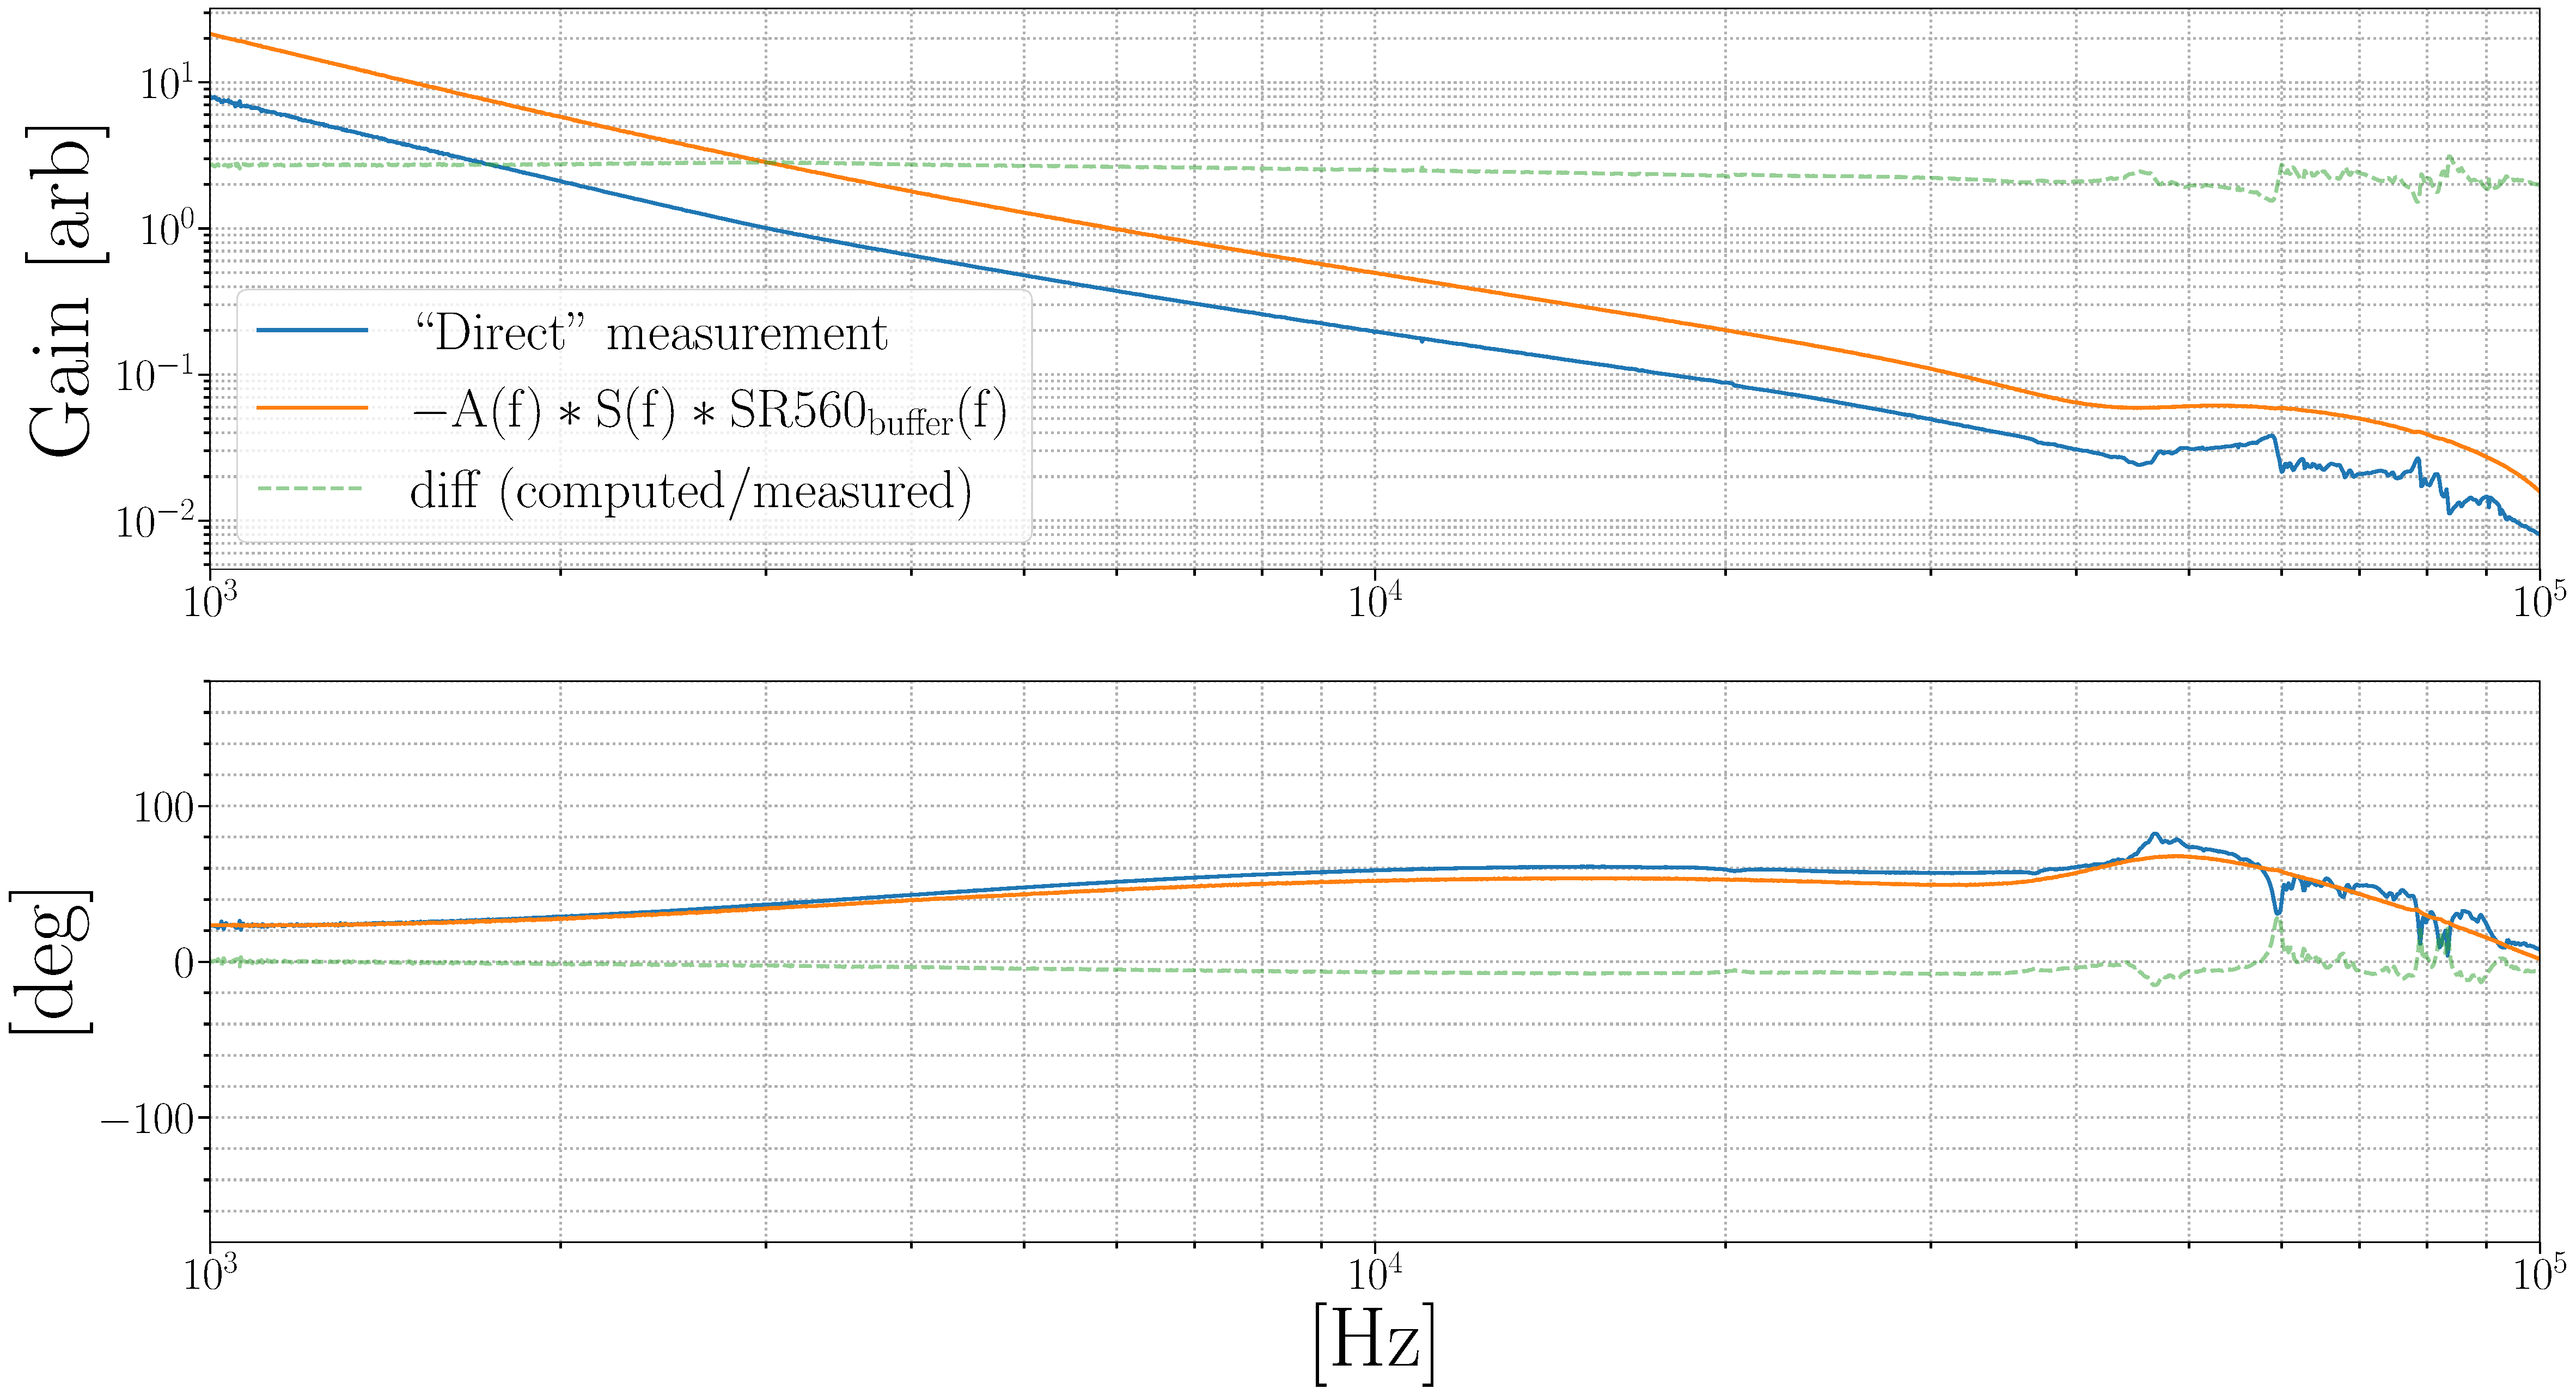
\includegraphics[width=\textwidth]{ALGAAS/olg_compare.pdf}
\end{center}
\caption{Comparison of the open loop gain measurement against the multiplied servo electronics measurements. The maximum gain difference is about a factor of 2.8 which is low passed to a difference of 2.0.}
\label{fig:OLG_compare}
\end{figure}


\subsection{Longitudinal Pockels Cell mirror mount assembly}
Maximizing a controlled and well defined electric field ($|E_z|$) within the coating while requiring a through beam to and through the HR coating lead us to a design very similar to that of a longitudinal pockels cell \cite{}. The most common assembly in for this study is comprised of two electrodes with a 3mm central aperture which is chosen to be at least 5 times larger than the beam size at the plate locations; to avoid significant beam clipping while maximizing field strength at the coating region of interest. There is also a required separation of at least 1/4" accounting for the thickness of the optical sample. Considering these constraints, modelling the system and computing the estimated field strength screened by the coating is the next step to the construction of the assembly.

\begin{figure}[H]
\begin{center}
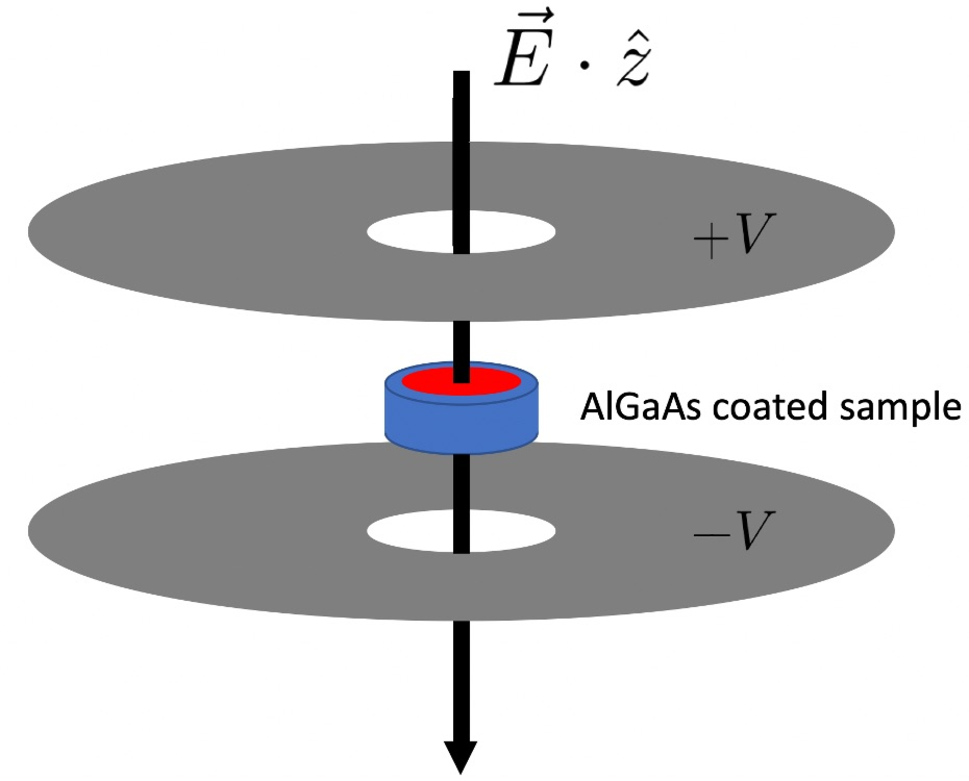
\includegraphics[width=.7\textwidth]{ALGAAS/assemblies/disk_electrode_concept.pdf}
\end{center}
\caption{Concept image of the longitudinal Pockels cell assembly}
\label{fig:pock_cell_assembly_concept}
\end{figure}

\subsubsection{Modelling}

To find the Electric field screened by the coating we begin with Gauss' Law:

\begin{equation}
\nabla \cdot D = \rho_\mathrm{free}
\end{equation}
For our problem we assume no free charge, but the fused silica substrate with the AlGaAs coating presents dielectric material between the plates. Our initial boundary conditions are also expressed in terms of plate potentials so it is natural to first solve for the potential ($V$) for every point within our system. We can exploit the cylindrical symmetry with the optic and plate geometry in the $r$ coordinate so we shall express the Laplacian accordingly:
\begin{equation}
\bigg[\frac{1}{r}\frac{\partial}{\partial r} \bigg( r \frac{\partial}{\partial r}\bigg) + \frac{\partial^2}{\partial z^2}\bigg](\varepsilon V) = 0
\end{equation}
Where $\varepsilon$ is the dielectric

\begin{figure}[H]
  \centering
  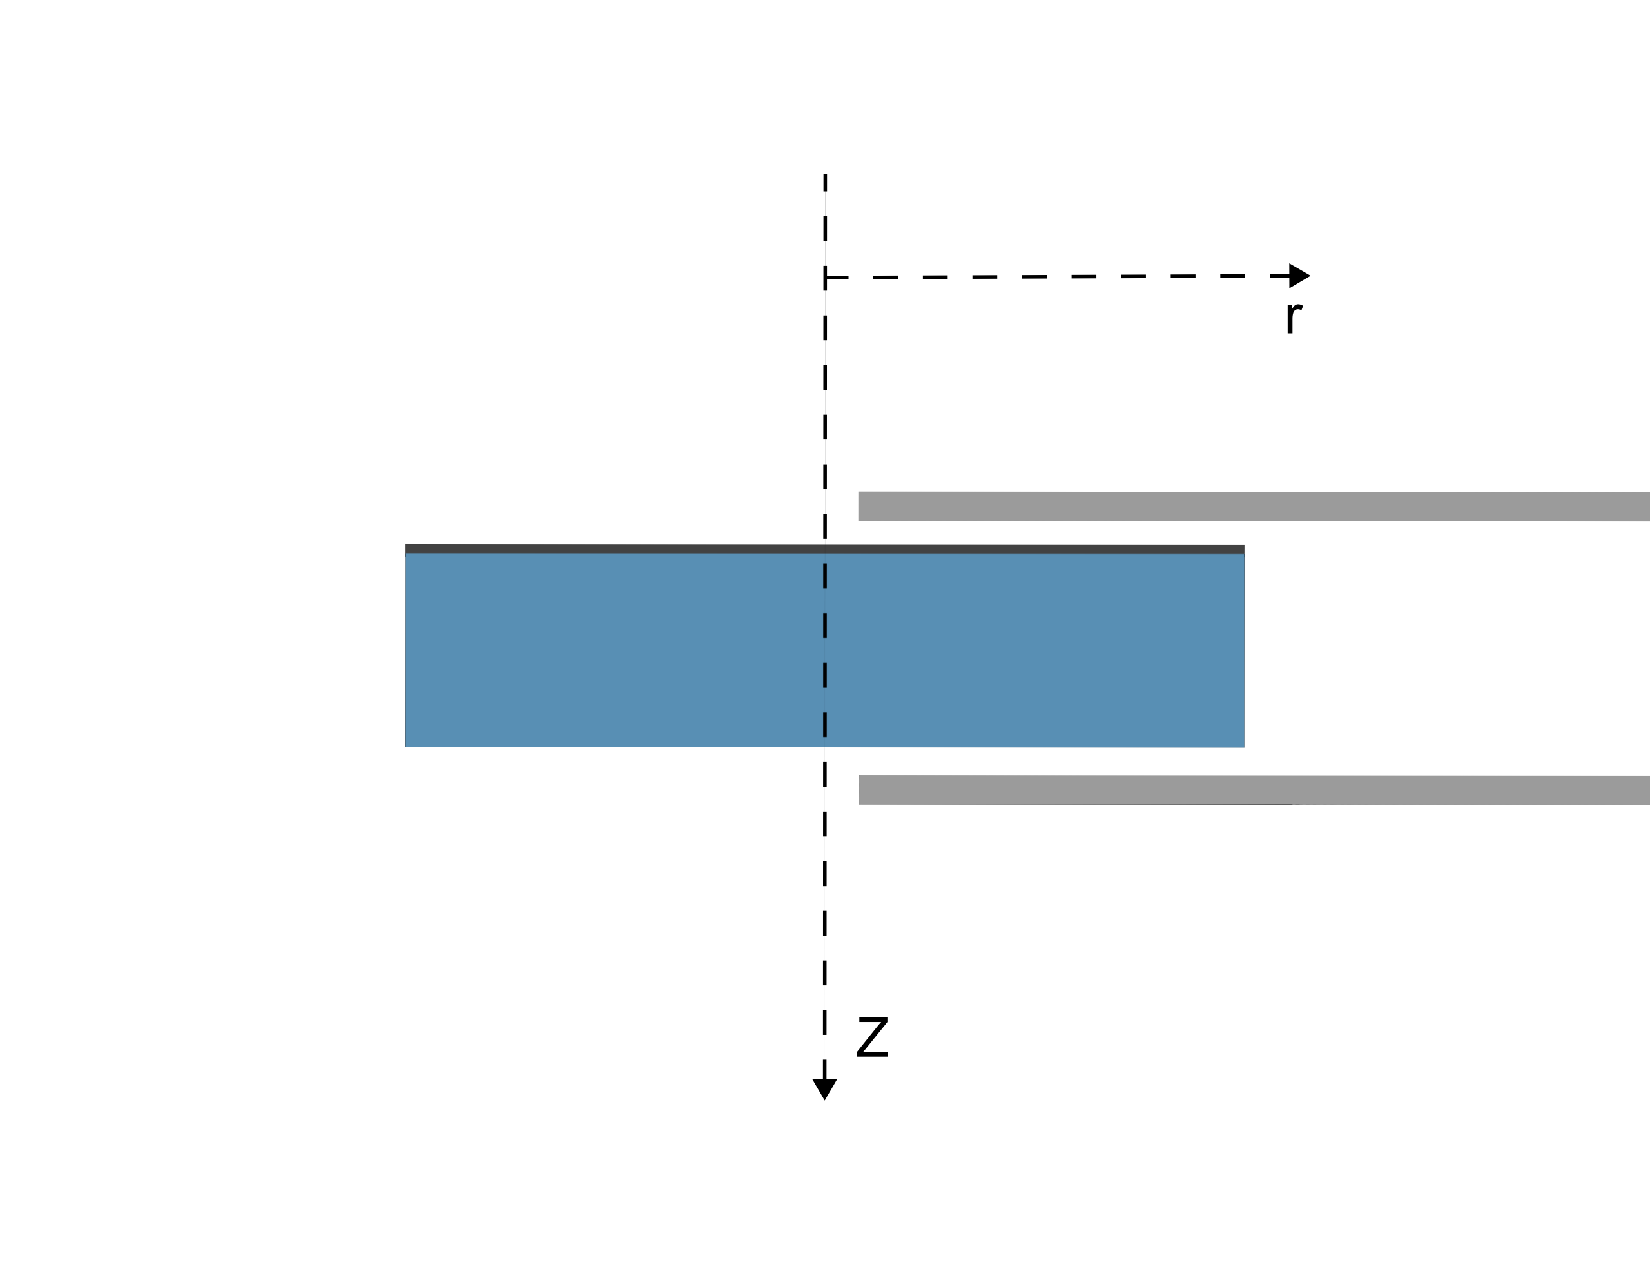
\includegraphics[width=.65\textwidth]{figs/ALGAAS/laplace_coord_test.pdf}
  \caption{\textcolor{red}{PENDING}}
  %%Use relevant cross sectional figure to establish coordinates for $\gaas$/$\algaas$, as well as the fused silica substrate so the computation is transparent.} Cross sectional diagram indicating relevant axes and boundary conditions utilized in the numerical computation
  \label{fig:laplace_coords}
\end{figure}

%%Numerical recipe in appendix

\begin{itemize}
\item Potential map computation in cylindrical
\item Computing $E_z$ from potential map
\begin{itemize}
\item inside coating
\item outside coating
\end{itemize}
\end{itemize}


\begin{figure}[H]
  \includegraphics[width=\textwidth]{ALGAAS/assembly1_sim.pdf}
  \caption{Poisson calculator output potential map ($V(z,r)$ in cylindrical coordinates)}
  \label{fig:poisson_calc_output}
\end{figure}

\subsubsection{Voltage drive electronics}

\begin{figure}[H]
    \includegraphics[width=\textwidth]{ALGAAS/13-Sep-2021_e_field_inside_outside_normal.pdf}
    \caption{The availablility of required voltage amplifiers during the course of this study was limited and lead to the use of multiple high voltage amplifiers with all transfer functions listed.}
\label{fig:Ez}
\end{figure}


\begin{figure}[H]
    \includegraphics[width=\textwidth]{ALGAAS/tfs/hva_compare.pdf}
    \caption{Different high voltage amplifier transfer functions used for the study}
    \label{fig:hva_compare}
\end{figure}

\section{Results}
Significant barriers were encountered in the form of cavity differential length noise especially when mounting the optics in accessible non-conductive materials. Most commercial optical mounts are constructed with conducting materials which proved to be a barrier when attempting to find a mounting solution while reducing non-normal field gradients within the coating volume of interest within the sample. For this reason, efforts were focused on developing a suitable mounting solution that would provide adequate isolation from any uncontrolled field magnitudes while driving a field normally incident on the surface with enough strength and uniformity across the beam area to extract a measurement of the differential length change from the Pockels effect. The mounts studied span different geometries and different material properties. The varying geometrical assembly differences created distinguishable mount solutions, and it is how this section will be divided. For reassurance, we compare displacement spectra against that of a nearly identical cavity with a flat non-crystalline mirror coating to perform a null measurement reference; ruling out the Pockels effect and providing information for noise investigations.

\subsection{Measurement Calibration}
The error signal spectra probed at the FSS:

\begin{equation}
\mathrm{VFSSOUT}_\mathrm{rms}/\sqrt{Hz} \rightarrow m_\mathrm{rms}/\sqrt{\mathrm{Hz}}
\end{equation}

With the known frequency response of the servo electronics, we \hyperref[sec:calibration]{calibrate} the measurement into differential length:
\begin{equation}
	\Delta \mathrm{L} = \mathrm{source}*\alpha(f) \mathrm{A}(f)*\frac{1+\mathrm{OLG}(f)}{\mathrm{OLG}(f)}*\frac{\mathrm{L_{cav}}}{f_\mathrm{laser}} \quad \big[ m_\mathrm{pk} / \sqrt{Hz} \big]
\end{equation}

\subsection{Mounting Strategies}
The following section details measurements performed with various longitudinal pockel cell mounts. Further details (assembly parameters, blueprints, and visual aids) can be found in the appendix.

\subsubsection{Assembly 1}

\begin{figure}[!ht]
    \begin{subcaptiongroup}
	    \includegraphics[width=.5\textwidth]{figs/ALGAAS/assemblies/assembly1/assembly1_dissassembled.pdf}
	    \phantomcaption\label{A1_disassembled}
	    \includegraphics[width=.5\textwidth]{figs/ALGAAS/assemblies/assembly1/assembly1_flaw.pdf}
	    \phantomcaption\label{A1_flaw}
    \end{subcaptiongroup}
    \caption{Assembly 1 was constructed to meet two criteria: the same solution of housing the sample and electrodes as Assembly 0, but also offer pitch / yaw control via an ortho-planar spring design (Brigham Young University).}
    \label{fig:A1pt0}
\end{figure}
\FloatBarrier


The construction revealed flaws; made most obvious when comparing to displacement noise of traditional optical mounts. Pitch and yaw control via the ortho-planar spring were prioritized to avoid metal springs and further mount pieces. The solution became unjustifiable when observing the the displacement noise coupling from the mount.

%%Re-run this calibration with adequate voltage normalization for a response unit [$m_\mathrm{pk} / [V / m]$]

\begin{figure}[H]
\centering
\includegraphics[width=\textwidth]{figs/ALGAAS/assemblies/assembly1/assembly1_2_compare_standmount.pdf}
\caption{Measured displacement spectra for Assembly 1.2 of the longitudinal pockels cell mount compared to the standard kinematic mount. Both measurements were recorded with the the CVI Melles-Griot (amorphous) mirror coating sample installed in the assembly.}
%%Units and legend labels need increase in font size. Remove Swept sine measurement title.
\label{fig:assembly2_compare_kinematic_mount}
\end{figure}


Attempts at improving the pitch dithering were tried with side set screws but mostly caused significant misalignment (less power in fundamental mode, locking issues, etc.). This lead to the final alternative for this assembly type; with the same PLA stack indicated in ~\hyperref[fig:A1pt0]{Assembly 1}.

\begin{figure}[!ht]
	\begin{subcaptiongroup}
		\includegraphics[width=.5\textwidth]{figs/ALGAAS/assemblies/assembly1/assembly1_mod_front.pdf}
		\phantomcaption\label{A1_front}
		\includegraphics[width=.5\textwidth]{figs/ALGAAS/assemblies/assembly1/assembly1_mod_side.pdf}
		\phantomcaption\label{A1_side}
	\end{subcaptiongroup}
    \caption{A modification implemented  with the intention of reducing pitch dithering while still having control of DC YAW}
    \label{fig:A1pt0mod}
\end{figure}

\begin{figure}[H]
    \includegraphics[width=\textwidth]{figs/ALGAAS/results_figs/assembly1/1_2_algaas_tfwcmb.pdf}
    \caption{Assembly 1.2 and 1.3 transfer function measurement and separate noise displacement spectra measurement with the $\gaas$/$\algaas$ sample installed. Measurements were taken from 3kHz up to 21kHz on using a Stanford Research 785 spectrum analyzer.}
    \label{fig:assembly1_2_and_1_3_displacement_spectra_algaas}
\end{figure}

\begin{figure}[H]
    \includegraphics[width=\textwidth]{figs/ALGAAS/results_figs/assembly1/1_2_cvi_compare_tfwcmb.pdf}
    \caption{Assembly 1.2 and 1.3 transfer function measurement and separate noise displacement spectra measurement with a CVI Melles Griot flat mirror sample ($R \approx $ sample installed. Measurements were taken from 1kHz up to 30kHz on using a Stanford Research 785 spectrum analyzer.}
    \label{fig:assembly1_2_and_1_3_displacement_spectra_cvi}
\end{figure}

\subsubsection{Assembly 2}

With considerations after Assembly 1, a more monolithic optical mount design with a simple geometry was imagined. PLA material compliance factoring to the seen drive noise. To see if it could be due to the compliance of the assembly material or printing, we tested this assembly design against different infills of PLA, PETG, and a version machined from solid PVC. With this modification, came also a different plate geometry. The assumption is the region of interest of the injection would not be heavily influenced by the non-circular plate geometry where it matters.

% Some citations:
%\cite{PINTO2015635}

%\begin{figure}[!ht]
%	\begin{subcaptiongroup}
%		\includegraphics[width=.5\textwidth]{figs/ALGAAS/assemblies/assembly2/assembly2_PVC.pdf}
%		\phantomcaption\label{A2_PVC}
%		\includegraphics[width=.5\textwidth]{figs/ALGAAS/assemblies/assembly2/assembly2_PVC.pdf}
%		\phantomcaption\label{A2_PVC}
%    	\end{subcaptiongroup}
%    \caption{An iteration of assembly 2 comprised of a PVC mount with two rectangular (1.1"X2") plates with a central aperture of 3mm}
%    \label{fig:assembly2}
%\end{figure}

\begin{figure}[H]
    \includegraphics[width=\textwidth]{figs/ALGAAS/results_figs/assembly2/2_0_compare_1_1.pdf} 
    \caption{Assembly 2.0 transfer function measurements compared to Assembly 1.1, Measurements were taken from 1kHz up to 30kHz on using a Stanford Research 785 spectrum analyzer.}
    \label{fig:assembly2and1_1}
\end{figure}


\begin{figure}[H]
    \includegraphics[width=\textwidth]{figs/ALGAAS/results_figs/assembly2/vary_da.pdf}
    \caption{The varied drive amplitudes input into the HVA to perform the following test}
    \label{fig:vary_da}
\end{figure}

\begin{figure}[H]
    \includegraphics[width=\textwidth]{figs/ALGAAS/results_figs/assembly2/vv53.pdf} 
    \caption{Assembly 2.0 transfer function measurements with varied drive amplitudes indicated in ~\ref{fig:vary_da}.}
    \label{fig:vv53}
\end{figure}


\begin{figure}[H]
    \includegraphics[width=\textwidth]{figs/ALGAAS/results_figs/assembly2/vary_daao.pdf}
    \caption{The varied drive amplitudes and offsets input into the HVA to perform the following test}
    \label{fig:vary_daao}
\end{figure}

\begin{figure}[H]
    \includegraphics[width=\textwidth]{figs/ALGAAS/results_figs/assembly2/vvao517.pdf} 
    \caption{Assembly 2.0 transfer function measurements with varied drive amplitudes and offsets indicated in ~\ref{fig:vary_daao}.}
    \label{fig:vvao517}
\end{figure}

\subsubsection{Assembly 3 (MACOR mount)}
With most of the same characteristics from Assembly 3, an optical mount made of MACOR, a machinable ceramic, was constructed and installed. With the material's high Young's modulus (66.9 GPa), and a moderate Poisson ratio (.29) \cite{macor} making it by far the most durable / non-conductive mounting solution tried.

An optical mount for the sample made with MACOR, along with glass bearnings .48 $\pm$ .01 cm $\diameter$  and a McMaster-Carr 8-32, 1/2" ceramic screw were used to clamp and suspend the optical sample. A 1.24" $\diameter$ hole was bored into the MACOR with a (\textcolor{red}{depth?}) depth so that there is a .351 $\pm$ mm clearance between the front and back surface of the sample to the electrode plates.

%%FIGURE: sample in-situ
\begin{figure}[!ht]
    \begin{subcaptiongroup}
	    \includegraphics[width=.5\textwidth]{figs/ALGAAS/assemblies/assembly3/assembly3_disassembled.pdf}
	    \phantomcaption\label{A3_disassembled}
	    \includegraphics[width=.5\textwidth]{figs/ALGAAS/assemblies/assembly3/assembly3_isometric.pdf}
	    \phantomcaption\label{A3_isometric}
    \end{subcaptiongroup}
    \caption{Assembly 3: \subref{A3_disassembled} disassembled configuration and \subref{A3_isometric} an isometric view of the assembled configuration.}
    \label{fig:assembly3}
\end{figure}


\begin{figure}[H]
    \includegraphics[width=\textwidth]{figs/ALGAAS/results_figs/assembly3/petgmsvv64.pdf}
    \caption{A polarization depdendent test using the MACOR mont}
    \label{fig:measurement_sum}
\end{figure}

\subsubsection{Opto-mechanical coupling}
During Assembly 2 tests the drive coupling seen in the transfer function measurements for all mounts tried was hypothesized to be due to mechanical action the assembly construction when driving the voltage on electrodes plates. Tracking consistent mechanical action for assemblies prior to Assembly 3 was difficult due to inconsistent mechanical settings between some measurements. More consistent measurements were realized when mechanical settings were tracked more carefully (i.e. set screw torque) and ceramic / glass materials used for suspending sample within the assembly. 
Sample and mount mechanical mode excitations. Seen with both AlGaAs and a HR coating from an AtFilm (IBS coating)
\begin{itemize}
\item \textbf{Vibration of plates (Leissa)} \cite{leissa} Computing frequencies and order of magnitude
\item \textbf{Steve's COMSOL model results}
\end{itemize}

\subsubsection{Dual-polarization locked configuration}

\subsection{Conclusion}


\chapter{Conclusion}

\chapter{Appendix}
% IFO configs (jupyter notebooks)

% Paraxial equation

% Cavity Stability criteria

% The Equipartition theorem and the Fluctuation Dissapation theorem

% Monochromatic plane wave propogation

% The Dielectric Tensor

% Thermo-optic Path Distortion (analytical)
% Transient thermo-optic responses
    %% Thermal Lens Optical Path Distortion (Hello-Vinet)
    %% COMSOL self heating filter
    %% RH actuation
	%%% Analytical solution
	%%% Conditioned RH input filter
    %% CO2 filters

% CO2 mask

% Mode matching data for Electro-optic sample cavity
    %% Pre MMT beam scan
    %% ``Just another mode matching tool" (JAMMT) solution
    %% Post MMT beam scan

% Laser PZT sweep

% Assembly blueprints and alternative views
    %% Assembly 1
	%%% Cross section
    	%%% Electrodes
    	%%% Iteration 1.1
    	%%% Iteration 1.2
    	%%% Iteration 1.3
    %% Assembly 2
	%%% Cross section
    	%%% Electrodes
    	%%% Iteration 2.1
    	%%% Iteration 2.2
    	%%% 3D printed with MACOR spacers
    %% Assembly 3
	%%% Cross section
    	%%% Electrodes
    	%%% Iteration 3.0

% LaplacE code
    %% laplacedotpy
    %% set\_paramsdotpy
    %% rundotipynb
% Calibration code

% HVA

% FSS

% Measuring OLG

\section{Interferometer configurations (code)}
\subsection{ifo\_configs.py}
\begin{spacing}{1}
\begin{lstlisting}[frame=single, language=Python]
import numpy as np

# Bode tools 
def bode_amp(H):
    """
    Returns amplitude information on transfer function (H)
    """
    return np.sqrt(np.real(H)**2 + np.imag(H)**2)

def bode_ph(H):
    """
    Returns phase information on transfer function (H)
    """
    return (180/np.pi)*np.arctan(np.imag(H)/np.real(H))

# some constants:
cee = np.float64(299792458) ## speed of light [m/s]
h_bar = (6.626e-34)/(2*np.pi) ## planck's constant


# IFO params
def finesse(r_i, r_e):
    """
    r_i : ITM reflectivity coefficient
    r_e : ETM reflectivity coefficient
    """
    return np.pi*np.sqrt(r_i*r_e)/(1-(r_i*r_e))


# Michelson frequency response
def mich_freq_resp(freq, Length, phi_0, P_in, OMEGA):
    """ 
    MICHELSON FREQEUNCY RESPONSE CALCULATOR
    freq : standard (gravitational wave) frequency [Hz]
    Length : Michelson ifo arm length [m]
    phi_0 : static differential arm length tuning phase [rad]
    P_in : input power [W] 
    """
    return (P_in*OMEGA*np.sin(phi_0))*Length*
	    np.exp((-1j*Length*2.0*np.pi*freq)/cee)*
	    np.sin((Length*2.0*np.pi*freq)/cee)/(Length*2.0*np.pi*freq)

def fpmi_freq_resp(freq, r_1, t_1, r_2, L, phi_0, P_in, OMEGA, low_pass=False):
    """
    FABRY PEROT MICHELSON FREQUENCY RESPONSE CALCULATOR
    freq : standard (gravitational wave) frequency [Hz]
    r_1, t_1, r_2: Assuming arm symmetry where the ITM has r_1, t_1 coefficients 
		   and the ETM has a r_2 reflectivity coefficient. 
		   Also assumes no loss. [arb]
    OMEGA: OPTICAL angular frequency [rad Hz]
    Length: Michelson ifo arm length [m]
    phi_0 : static differential arm length tuning phase [rad]
    """
    if low_pass:
        f_pole = 1/(((4*np.pi*L)*np.sqrt(r_1*r_2))/(cee*(1-r_1*r_2)))
        fpmi_resp = 1/(1 + 1j*(freq/f_pole))
    else:
        fpmi_resp = ((t_1**2 * r_2)/((t_1**2 + r_1**2)*r_2 - r_1))*
		    (mich_freq_resp(freq, L, phi_0, P_in, OMEGA)/
		    (1-r_1*r_2*np.exp(-1j*L*4.0*np.pi*freq/cee)))
    return fpmi_resp

def PRG(L_rt, Finn, r_PRM, max=0):
    """
    POWER RECYCLING GAIN (@ optimal reflectivity)
    * Assuming a FPMI with symmetric arms *
    L_rt : Round trip loss
    Finn : Cavity finesse
    """
    if max == 1:
        G_PR = np.pi/(2*Finn*L_rt*(1-((Finn*L_rt)/(2*np.pi))))
    else:
        G_PR = (1-r_PRM**2)/(1-r_PRM*(1-(Finn/np.pi)*L_rt))**2


    return G_PR

def drfpmi_freq_resp(freq, G_PRC_opt, r_1, t_1, r_2, r_SRM, t_SRM, phi_SRC, L, 
		     phi_0, P_in, OMEGA):
    """
    DUAL RECYCLED FABRY PEROT MICHELSON FREQUENCY RESPONSE 
    CALCULATOR

    freq: standard (gravitational wave) frequency [Hz]
    G_PRC_opt: maximum power recycling gain (optimal) [arb]
    r_1: ITM reflection coefficient [arb]
    t_1: ITM transmission coefficient [arb]
    r_2: ETM reflection coefficient [arb]
    r_SRM: Signal recycling mirror reflection coefficient [arb]
    t_SRM: Signal recycling mirror transmission coefficient [arb]
    L: Length of the Fabry-Perot arms [m]
    OMEGA: OPTICAL angular frequency [rad Hz]
    """
    r_SRC = (r_1 - r_SRM*np.exp(1j*2*phi_SRC))/
	    (1 - r_1*r_SRM*np.exp(1j*2*phi_SRC))
    t_SRC = t_1*t_SRM*np.exp(1j*phi_SRC)/(1 - r_1*r_SRM*np.exp(1j*2*phi_SRC))

    return ((t_1**2 * r_2)/((t_1**2 + r_1**2)*r_2 - r_1))*
	    G_PRC_opt*t_SRC*(P_in*L*OMEGA*np.exp((-1j*L*2.0*np.pi*freq)/cee)*
	    np.sin((L*2.0*np.pi*freq)/cee)/(L*2.0*np.pi*freq))/
	    (1-r_SRC*r_2*np.exp(-1j*L*4.0*np.pi*freq/cee))


# Shot noise
def N_shot(OMEGA, P_in):
    """
    Interferometer shot noise calculator
    OMEG: OPTICAL angular frequency [rad Hz]
    Length : ifo arm length [m]
    phi_0 : static differential arm length tuning phase [rad]
    P_in : Input power [W]
    """
    return np.sqrt(2*h_bar*OMEGA*P_in)
\end{lstlisting}
\end{spacing}


\subsection{MICH}
\begin{spacing}{1.2} \begin{lstlisting}[frame=single, language=Python]
import numpy as np
import matplotlib.pyplot as plt
import os
import sys
sys.path.insert(0,'../')
plt_style_dir = '../../stash/'
fig_exp_dir = '../../../figs/'
from ifo_configs import N_shot
from ifo_configs import mich_freq_resp as MICH
from ifo_configs import bode_amp, bode_ph
%matplotlib inline
if os.path.isdir(plt_style_dir) == True:
    plt.style.use(plt_style_dir + 'ppt2latexsubfig.mplstyle')
plt.rcParams["font.family"] = "Times New Roman"
\end{lstlisting} \end{spacing}

\begin{spacing}{1.2} \begin{lstlisting}[frame=single, language=Python]
# Some parameters
cee = np.float64(299792458)
h_bar = (6.626e-34)/(2*np.pi)
OMEG = np.float64(2*np.pi*cee/(1064.0*1e-9))
L = np.float64(4000.0)
nu = np.arange(1, 1000000, 1)
PHI_0 = np.pi/2 #[rad]
P_IN = 125 #[W]
\end{lstlisting} \end{spacing}

\hypertarget{derivation}{%
\subsubsection{Derivation}\label{derivation}}

For the simple Michelson we know that a change in arm length correlates
to light at the AS port We also know that a differential arm length
corresponds to a difference in phase of the light that impinges upon the
BS For a gravitational wave we can quantify the phase difference in this
following way:

\begin{equation}
\phi_A - \phi_B = \int_{t-2L/c}^{t} \Omega \bigg[1 + \frac{1}{2}h(t)\bigg]dt - \int_{t-2L/c}^{t} \Omega \bigg[1 - \frac{1}{2}h(t)\bigg]dt 
\end{equation} The phase difference can then be quantified by: \begin{equation}
\phi_A - \phi_B = \int_{t-2L/c}^{t} \Omega h(t)dt 
\end{equation} where \begin{equation} 
h(t) = h_0 e^{i \omega t} 
\end{equation}

\noindent \emph{\(\Omega\)} is the \textbf{optical angular frequency}

\noindent After evaluating this integral we get: 
\begin{equation}
\Delta \phi=\phi_A - \phi_B = \frac{2 L \Omega}{c}e^{-i L \omega / c} \frac{\mathrm{sin}(L \omega /c)}{L \omega /c} \cdot h_0 e^{i \omega t}
\end{equation}

\noindent Where the first term in the phase difference carries all the time
independent frequency information. This is what we are calculating
below.

\noindent For the sake of being explicit, we are going to plot: 
\begin{equation}
\Delta \phi (\omega) = h_0\frac{2 L \Omega}{c}e^{-i L \omega / c} \frac{\mathrm{sin}(L \omega /c)}{L \omega /c}
\end{equation}This accounts for the differential phase as a function of
gravitational wave frequency, though we have not established the amount
of optical gain the Michelson offers. This can be understood through a
first order taylor approximation about a selected Michelson offset angle
\(\phi_0\):

\begin{equation}P(\omega, \phi_0) =  \frac{P_\mathrm{in}}{4} [r_x^2 + r_y^2 -  2r_x r_y\mathrm{cos}(\phi_0 + \Delta \phi (\omega)] \end{equation}

\begin{equation}P(\omega, \phi_0) \approx  \frac{P_\mathrm{in}}{4} \Big[ r_x^2 + r_y^2 -  2r_x r_y \big(\mathrm{cos}(\phi_0) - \Delta \phi(\omega) \cdot \mathrm{sin}(\phi_0) \big) \Big] =  \frac{P_\mathrm{in}}{2} \Big[1 - \big(\mathrm{cos}(\phi_0) - \Delta \phi(\omega) \cdot \mathrm{sin}(\phi_0) \big) \Big]\end{equation}

\noindent Where we define a response gain function \(H_\mathrm{MICH}\):

\begin{equation}\mathrm{H}_\mathrm{MICH}(\omega, \phi_0) =   \frac{P_\mathrm{in}}{2} \cdot \Delta \phi(\omega) \cdot \mathrm{sin}(\phi_0)\end{equation}

\begin{spacing}{1.2} \begin{lstlisting}[frame=single, language=Python]
H = MICH(nu, L, PHI_0, P_IN, OMEG)
\end{lstlisting} \end{spacing}

\begin{spacing}{1.2} \begin{lstlisting}[frame=single, language=Python]
fig, ax1 = plt.subplots()
ax1.set_xlabel('frequency [Hz]')
ax1.set_ylabel('H$_{\mathdefault{MICH}}$ [$\mathdefault{W/m}$]',color='C0')
#ax1.plot(w/(FSR), F_w_cc_modsq*100)
ax1.loglog(bode_amp(H),linewidth=7.5, color='C0')
#plt.ylim([10e-6, 10e0])
ax2 = ax1.twinx()
#ax2.plot(w/(FSR), (180/np.pi)*np.arctan(F_w_cc.imag/F_w_cc.real), '--')
ax2.semilogx(nu,(180/np.pi)*np.arctan(np.imag(H)/np.real(H)), '--', linewidth=7.5,
	     color='C1')
#plt.xlabel('frequency [FSR]')
plt.xlim([1,1e5])
plt.ylabel('phase [deg]',color='C1')
fig.savefig(fig_exp_dir + 'INTRO/mich_fr.pdf', dpi=300, bbox_inches='tight')
\end{lstlisting} \end{spacing}

Though with the provided frequency depdenence and optical gain, we still
need to understand a starting noise floor spectra and compare to our
anticipated limiting noise 

\noindent\textbf{Shot noise} 
\\
* A fundamental limit imposed by the statistical nature of photon counting 
\\
* The photon counting follows Poisson statistics 
\\
\indent    * Photon counting variance (variance is equal to the
mean) 
\begin{equation} < (n-\bar{n})^2 >  = \frac{P \Delta t}{ \hbar \Omega} \end{equation} 
\indent * Power variance:
\begin{equation} < (P - \bar{P})^2 >  = \hbar \Omega  \bar{P} \Delta t \end{equation} 
\indent * PSD of the measured power between two uncoorelated moments in time:
\begin{equation} S_\mathrm{P} (\omega) = \lim_{T \to \infty} \frac{2}{T} \Big< \big| \int_{-T}^{T} (P(t) - \bar{P}) e^{-i\omega t} dt \big|^2 \Big> \end{equation}
\begin{equation} =  \lim_{T \to \infty} \frac{2}{T} \int_{-T}^{T} \hbar \Omega \bar{P} dt  \end{equation}
\begin{equation} = 2 \hbar \Omega \bar{P} \end{equation} 
\indent * Where the ASD is:
\begin{equation} [S_P (\omega)]^{1/2} = [2 \hbar \Omega \bar{P}]^{1/2}\end{equation}The signal to
noise is established by dividing the frequency dependent optical gain
times the gravitational wave ASD
\(\big( [\mathrm{S}_{\mathrm{h}}(\Omega)]^{1/2} \big)\) by the noise
ASD:

\begin{equation}\mathrm{SNR} = \mathrm{G_{opt}(\omega)} [\mathrm{S}_{\mathrm{h}}(\omega)]^{1/2} / S_\mathrm{N}(\omega) = \mathrm{H}_\mathrm{MICH} / [S_P]^{1/2} = \bigg( \frac{\Delta \phi(\omega)}{h_0} \frac{P_\mathrm{in}}{2}\mathrm{sin}(\phi_0) \bigg) \bigg/ [2 \hbar \Omega \bar{P}]^{1/2}\end{equation}

\noindent This is to say that for the stated gravitational wave ASD, and for an
SNR of 1, we establish the following threshold for detector:

\begin{equation}\big[ \mathrm{S}_{\mathrm{h}}(\omega) \big]^{1/2} \; \{\mathrm{SNR}\geq1\} \geq \frac{ [S_\mathrm{N}(\omega)]^{1/2}}{\mathrm{H}_\mathrm{MICH}(\omega)}\end{equation}

\noindent Where

\begin{equation}\frac{ [S_\mathrm{N}(\omega)]^{1/2}}{\mathrm{H}_\mathrm{MICH}(\omega)} = \frac{[2 \hbar \omega \bar{P}]^{1/2}}{ \Delta \phi(\omega) [P_\mathrm{in} / 2]  \mathrm{sin}(\phi_0)} = \bigg( \frac{\hbar \Omega }{\omega P_\mathrm{in}} \bigg)^{1/2} \frac{[r_x^2 + r_y^2 -  2r_x r_y\mathrm{cos}(\phi_0)]^{1/2}}{\mathrm{sin}(L \omega / c)} e^{iL \omega / c}\end{equation}

\begin{spacing}{1.2} \begin{lstlisting}[frame=single, language=Python]
S_h = N_shot(OMEG, P_IN) 
print(S_h)
\end{lstlisting} \end{spacing}

\begin{spacing}{1.2} \begin{lstlisting}[frame=single, language=Python]
#ax1.plot(w/(FSR), F_w_cc_modsq*100)
plt.loglog(nu, S_h/bode_amp(H), linewidth=7.5, color='C0')
plt.ylim([1e-21, .5e-14])
plt.xlabel('frequency [Hz]')
plt.ylabel('$\mathdefault{S}_\mathdefault{h} \;  
	    \mathdefault{[ 1 / \sqrt{\mathdefault{Hz}}]} $')
#ax2_ = ax1_.twinx()
#ax2.plot(w/(FSR), (180/np.pi)*np.arctan(F_w_cc.imag/F_w_cc.real), '--')
#ax2_.semilogx(nu,(180/np.pi)*np.arctan(np.imag(S_h)/np.real(S_h)), '--', 
	       linewidth=7.5,color='C1')
#plt.xlabel('frequency [FSR]')
plt.xlim([1,1e5])
plt.grid(visible=True)
#plt.subplots_adjust(hspace = 1)
#plt.ylabel('phase [deg]',color='C1')
#plt.tight_layout(rect=[0,0,1,1])
#plt.title('')
#plt.subplots_adjust(bottom=.1, top=.85) #, right=.8, left=.1)
plt.savefig(fig_exp_dir + 'INTRO/mich_sensi.pdf', dpi=300, bbox_inches='tight')
\end{lstlisting} \end{spacing}



\subsection{FPMI}
\begin{lstlisting}[frame=single, language=Python]
import numpy as np 
import matplotlib.pyplot as plt
import scipy.signal as sig
import os
import sys
sys.path.insert(0,'../')
plt_style_dir = '../../stash/'
fig_exp_dir = '../../../figs/'
from ifo_configs import mich_freq_resp as MICH
from ifo_configs import fpmi_freq_resp as FPMI
from ifo_configs import N_shot, bode_amp, bode_ph
if os.path.isdir(plt_style_dir) == True:
    plt.style.use(plt_style_dir + 'ppt2latexsubfig.mplstyle')
plt.rcParams["font.family"] = "Times New Roman"
line_width=7.5
\end{lstlisting}

Let's start with the simple Fabry Perót cavity. The following are
equations that characterize the circulating and reflected fields (both
critical to measuring the phase response of the FP cavity to GWs):

\[
E(t) = t_1 E_{in} + r_1 r_2 E(t - 2T) e^{-i \Delta \phi(t)} 
\]

\[
E_r(t) = -r_1 E_{in} + t_1 r_2 E(t - 2T) e^{-i \Delta \phi(t)}
\]

\(T = L/c\) is the time it takes light to reach the end of the cavity
and \(\Delta \phi(t)\) is the phase rotation.

We can define the static phase rotation (no GW passing through) as :
\[\Delta \phi = 2kL = 4 \pi L /\lambda_{opt}  \]

And if L is tuned just right \(2kL = 2 \pi n\) so the cavity is just
tuned for resonance

If we put a gravitational wave in the mix we redefine this phase
rotation as such that:
\[\Delta \phi =  \frac{\omega_0}{2} \int_{t-\frac{2L}{c}}^{t} h(t')dt' \]

This assumes that the static phase rotation satisfies
\(2\omega_0L/c = 2 \pi n\). Which is the same thing that we said above
but with different symbols (because we're fancy ;D )

Say that we have something that does throw the cavity slightly off
resonance.. doesn't have to be a gravitational wave\ldots{} but that's
what we hope for. ANYWAY\ldots{}

If the \(\Delta \phi\) becomes such that the cavity is thrown off
resonance we get a time dependent intra-cavity field:

\[ E(t) = \bar{E} + \delta E(t) \]

and if the phase rotation (\(\Delta \phi\)) is super small\ldots{} which
is pretty much guaranteed with gravy waves, we can say:

\[ e^{i\Delta \phi} = 1- i \Delta \phi \]

Using equations \ref{eq7} and \ref{eq8} in \ref{eq3} we get:

\[ \bar{E} + \delta E(t) = t_1 E_{in} -r_1r_2\bar{E} + r_1r_2 \delta E(t-2T) - ir_1r_2\bar{E}\Delta \phi(t)) \]

We can parse this into time dependent and time independent terms:

\[ \bar{E} = t_1 E_{in} -r_1r_2\bar{E} \]

\[ \delta E(t) = r_1r_2 \delta E(t-2T) - ir_1r_2\bar{E}\Delta \phi(t) \]

Since the time dependent phase information is encoded in \ref{eq11} we
will take the laplace transform of this equation to yield:

\[\delta E(s) = -i \frac{r_1r_2 \bar{E}}{1-r_1r_2e^{-2sT}} \Delta \phi(s)\]

\textbf{YAS!} we are now one step closer to getting a useful expression
for the phase response. But again.. what does this last equation mean?
That last equation is how the change in the electric field directly
relates to a small perturbation in phase (which could be either a small
change in laser frequency or length modulation)

Now.. we're not done yet because that last expression does not tell us
the entire story yet.. we want to see how this effects the phase
differential with the \textbf{reflected} electric field.

To do this.. we have to combine equations \ref{eq3} and \ref{eq4}. (an
easy way to do this is to get rid of the $ r_2 E(t - 2T) e^{-i \Delta \phi(t)} $ ) :

\[ E_r(t) = \frac{t_1}{r_1}E(t) - \frac{t_1^2 + r_2^2}{r_1} E_{in}\]

if the cavity is unperturbed:

\[ \bar{E}_r = \bigg(\frac{r_2(r_1^2 + t_1^2) - r_1}{t_1} \bigg) \bar{E} \]

and if we perturb the cavity we see that the change in the intra-cavity
field is directly related to the change in the reflected field:

\[ \Delta \phi_r(s) \equiv \frac{\delta E(s)}{\bar{E}} = \frac{t_1^2r_2}{(t_1^2 + r_1^2)r_2 -r_1} \frac{\Delta \phi(s)}{1-r_1r_2e^{-2sT}}\]

This implies that there is an additional frequency dependent factor in
your phase shift and this translates into your FPMI transfer function
as:

\[ H_{FPMI}(\omega_g) = \frac{2 \Delta \phi_r(\omega_g)}{h(\omega_g)} =  \frac{t_1^2r_2}{(t_1^2 + r_1^2)r_2 -r_1} \frac{H_{\mathrm{MI}}(\omega_g, L)}{1-r_1r_2e^{-2i \omega_g L /c }}  \]

Whew\ldots. that was a lot\ldots. now let's code it up Since we can
seperate the calculation into two.. I'm going to parse out the
calculation between the constant Fabry Perót term and the term with the
frequency dependence. But first, lets set up our parameters for our
FPMI:

\begin{lstlisting}[frame=single, language=Python]
# Some parameters
cee = np.float64(299792458)
OMEG = np.float64(2*np.pi*cee/(1064.0*1e-9))
L = np.float64(4000.0)
nu = np.arange(1, 1000000, 1)
nat_nu = [np.float64(i*2*np.pi) for i in nu]
h_0 = np.float64(1)

PHI_0 = np.pi/2 #[rad]
P_IN = 25

T_1 = .014
#T_1 = 25e-6 
T_2 = 50e-6
R_1 = 1-T_1
R_2 = 1-T_2

t_1 = T_1**.5
r_1 = R_1**.5
r_2 = R_2**.5
\end{lstlisting}

Now we can compute:
\[ H_{FPMI}(\omega_g) =  \frac{t_1^2r_2}{(t_1^2 + r_1^2)r_2 -r_1}\cdot \frac{H_{\mathrm{MI}}(\omega_g, L)}{1-r_1r_2e^{-2i \omega_g L /c }}  \]

\begin{lstlisting}[frame=single, language=Python]
H_FPMI = FPMI(nu, r_1, t_1, r_2, L, PHI_0, P_IN, OMEG)
\end{lstlisting}

We estimate the FP's pole frequency
\[  1 - r_1 r_2 e^{-2i \omega_g L / c} = 0 \] therefore when:
\[ e^{-i \omega_g L / c} = \frac{1}{\sqrt{r_1 r_2}} \] we acquire the
pole frequency \(\omega_\mathrm{pole}\) as indicated in the low pass
\[ f_\mathrm{pole} = \frac{1}{4\pi \tau_{s}} =  \frac{c}{4 \pi L} \frac{1- r_1 r_2}{\sqrt{r_1 r_2}} = \frac{\nu_\mathrm{FSR}}{2 \pi} \frac{1- r_1 r_2}{\sqrt{r_1 r_2}} = \frac{\nu_\mathrm{FSR}}{\mathcal{F}} \]

ALso, understanding that the cavity Finesse can be defined as

\[ \mathcal{F} = \frac{\pi \sqrt{r_i r_e}}{1- r_i r_e} \]

we also can invert for a high value of finesse $ \mathcal{F} \textgreater\textgreater{} \pi $:

\[ r_i r_e \approx 1 - \frac{\pi}{\mathcal{F}} \]

\begin{lstlisting}[frame=single, language=Python]
f_pole = 1/(((4*np.pi*L)*np.sqrt(r_1*r_2))/(cee*(1-r_1*r_2)))
def fpmi_lp(freq, cav_pole):
    return 1/(1 + 1j*(freq/cav_pole))#*np.exp(1j*freq/cav_pole))
H_FPMI_LP = fpmi_lp(nu, f_pole)
\end{lstlisting}

Might as well compare it to our Michelson response:
\[ H_{\mathrm{MI}}(\omega_g) = \frac{2 L \Omega}{c}e^{-i L \omega / c} \frac{\mathrm{sin}(L \omega /c)}{L \omega /c} \]

\begin{lstlisting}[frame=single, language=Python]
H_MICH = MICH(nu, L, PHI_0, P_IN, OMEG)
\end{lstlisting}

\begin{lstlisting}[frame=single, language=Python]
fig, ax1 = plt.subplots()
ax1.set_xlabel('frequency [Hz]')
ax1.set_ylabel('H$_\mathdefault{FPMI} \; \mathdefault{ [W / m] } $ ', color='C0')
#ax1.plot(w/(FSR), F_w_cc_modsq*100)
ax1.loglog(bode_amp(H_FPMI), label='FPMI', linewidth=line_width,color='C0')
#ax1.loglog(w,H_MI_modsq, label= 'MICH', linewidth= 5)
#ax1.loglog(w,H_FPMI_LP_modsq*H_FPMI_modsq[0], label='FPMI LP', 
	    linewidth = 20.0, alpha=0.25,color='C2')
#ax1.axvline (x=f_pole,ymin=1e-13, color='red', linestyle='dotted', linewidth=3)
ax2 = ax1.twinx()
ax2.semilogx(nu,bode_ph(H_FPMI),'--', linewidth=line_width, color='C1')
#ax2.semilogx(w,(180/np.pi)*np.arctan(np.imag(H_MI)/np.real(H_MI)), '--')
#ax2.semilogx(w,(180/np.pi)*np.arctan(np.imag(H_FPMI_LP)/np.real(H_FPMI_LP)),
	      linestyle='--', linewidth=20.0,dashes=(4,10),alpha=.25, color='C2')
plt.xlim([1,1e5])
plt.ylabel('phase [deg]', color='C1')
#fig.savefig('../figs/INTRO/fpmi_fr.pdf', dpi=300, bbox_inches='tight')
\end{lstlisting}

\begin{lstlisting}
Text(0, 0.5, 'phase [deg]')
\end{lstlisting}

\begin{lstlisting}[frame=single, language=Python]
plt.loglog(nu,bode_amp(H_MICH), label= 'MICH', linewidth= line_width, alpha=.5)
plt.loglog(nu,bode_amp(H_FPMI), label='FPMI', linewidth=line_width)
#plt.loglog(nu,bode_amp(H_FPMI_LP)*bode_amp(H_FPMI)[0], label='FPMI LP', 
	    linewidth = 20.0, alpha=0.25)
plt.axvline (x=f_pole,ymin=1e-11, color='red', linestyle='dotted', linewidth=3.0)
plt.ylim([5e7, 5e14])
plt.xlim([1e0, 1e5])
#plt.grid(visible=True, which='minor', axis='y')
plt.xlabel('frequency [Hz]')
plt.ylabel('H(f) $\mathdefault{[W/m]}$')
lgd=plt.legend()
plt.savefig('../figs/INTRO/fpmi_fr.pdf', dpi=300, bbox_inches='tight')
\end{lstlisting}

You can clearly see that there is a clear increase in gain at lower
frequencies (below 5000 kHz) Doesn't exactly look like Kiwamu's but
close enough?

\begin{lstlisting}[frame=single, language=Python]
plt.semilogx(nu,bode_ph(H_MICH), '--', label='MICH', linewidth= line_width, alpha=.5)
plt.semilogx(nu,bode_ph(H_FPMI),'--', label='FPMI', linewidth= line_width)
#plt.semilogx(nu,bode_ph(H_FPMI_LP),linestyle='--', linewidth=3.0,dashes=(3,10))
plt.xlim([1,100000])
plt.ylabel('phase [deg]')
plt.xlabel('Frequency [Hz]' )
lgd=plt.legend()
\end{lstlisting}

\begin{lstlisting}[frame=single, language=Python]
Sh_noise = N_shot(OMEG, P_IN)
\end{lstlisting}

\begin{lstlisting}[frame=single, language=Python]
plt.loglog(nu,Sh_noise/bode_amp(H_MICH), label= 'MICH', 
	   linewidth= line_width, alpha=.5)
plt.loglog(nu,Sh_noise/bode_amp(H_FPMI), label='FPMI', linewidth=line_width)
#plt.loglog(nu,Sh_noise/(bode_amp(H_FPMI_LP)*bode_amp(H_FPMI)[0]), 
	    label='FPMI LP', linewidth = 20.0, alpha=0.25)
#plt.axvline (x=f_pole,ymin=1e-11, color='red', linestyle='dotted', linewidth=3)
plt.ylim([1e-23, 1e-16])
plt.xlim([1e0, 1e5])
plt.xlabel('frequency [Hz]')
plt.ylabel('H(f) $\mathdefault{[1/\sqrt{\mathdefault{Hz}}]}$')
lgd=plt.legend()
fig.savefig('../figs/INTRO/fpmi_sensi.pdf', dpi=300, bbox_inches='tight')
\end{lstlisting}

\hypertarget{heavily-heavily-inspired-by-kiwamus-thesis-chapter-on-this-subject-httpsgwic.ligo.orgthesisprize2012izumi-thesis.pdf}{%
\subsubsection{*Heavily HEAVILY inspired by Kiwamu's thesis chapter on
this subject
(https://gwic.ligo.org/thesisprize/2012/izumi-thesis.pdf)}\label{heavily-heavily-inspired-by-kiwamus-thesis-chapter-on-this-subject-httpsgwic.ligo.orgthesisprize2012izumi-thesis.pdf}}


\subsection{DRFPMI}\label{appendix:DRFPMI}
\begin{lstlisting}[frame=single, language=Python]
import numpy as np 
import matplotlib.pyplot as plt
import scipy.signal as sig
import os 
import sys
sys.path.insert(0,'../')
plt_style_dir = '../../stash/'
fig_exp_dir = '../../../figs/'
import ifo_configs as ifco
if os.path.isdir(plt_style_dir) == True:
    plt.style.use(plt_style_dir + 'ppt2latexsubfig.mplstyle')
plt.rcParams["font.family"] = "serif"
plt.rcParams["font.serif"] = ["Times New Roman"] + plt.rcParams["font.serif"]
line_width=7.5
\end{lstlisting}

Up to this point we can understand how the FPMI repsonse function works:
\[ H_{FPMI}(\omega_g) = \frac{2 \Delta \phi_r(\omega_g)}{h(\omega_g)} =  \frac{t_1^2r_2}{(t_1^2 + r_1^2)r_2 -r_1} \frac{H_{\mathrm{MI}}(\omega_g, L)}{1-r_1r_2e^{-2i \omega_g L /c }}  \]

\begin{lstlisting}[frame=single, language=Python]
# Some parameters
cee = np.float64(299792458)
OMEG = np.float64(2*np.pi*cee/(1064.0*1e-9))
L = np.float64(4000.0)
nu = np.arange(1, 1000000, 1)
nat_nu = [np.float64(i*2*np.pi) for i in nu]
h_0 = np.float64(1)

T_1 = .014
#T_1 = 25e-6 
T_2 = 50e-6
R_1 = 1-T_1
R_2 = 1-T_2

t_1 = T_1**.5
r_1 = R_1**.5
r_2 = R_2**.5 

PHI_0 = np.pi/2 
P_IN = 25
\end{lstlisting}

\subsection{POWER RECYCLING}

With all the power going to the symmetric port, the nominal operating
state of the FPMI involves a significant amount of dumped / wasted
power. Placing a mirror at the symmetric port can allow that power to be
recycled. Though considerations must be made to maximize the amount of
recycling gain you can acquire with your GW detector. This is dependent
on the placement of the power recycling mirror (PRM) and its
reflectivity, transmission, and loss coefficients.

But first, the field at the symmetric port:

\[E_\mathrm{SYM} = \frac{E_i}{2}e^{2ikl}(r_\mathrm{FP,X} + r_\mathrm{FP,Y}) \]

This is realized through observing the circulating power between the PRM
and the short Michelson:

\[ E_\mathrm{PRC} = \frac{t_\mathrm{PRM}}{1- r_\mathrm{PRM} r_\mathrm{FPMI} e^{2ik (L_\mathrm{PRC2BS} + L_\mathrm{SMICH})}}E_\mathrm{in} \]

Where:

\[ L_\mathrm{SMICH} = l_x + l_y \]

Now let's observe the cavity reflection parameter:

\[ r_\mathrm{FP} = -r_1 + \frac{t_1^2 r_2 e^{i2kL}}{1-r_1 r_2 e^{i2kL}} = -\frac{\mathcal{F}}{\pi} \Big[-\Big(\frac{r_1}{r_2} \Big)^{1/2} + \Big(\frac{r_2}{r_1}\Big)^{1/2} (r_1^2 + t_1^2) \Big]\]
But with loss considerations:

\[ r_\mathrm{FP} = -r_1 + \frac{t_1^2 r_2 e^{- t_\mathrm{RT}/\tau_\mathrm{loss}}  e^{i2kL}}{1-r_1 r_2 e^{- t_\mathrm{RT}/\tau_\mathrm{loss}} e^{i2kL}} \approx -\frac{\mathcal{F}}{\pi} \Big[\frac{-r_1 +  r_2(r_1^2 + t_1^2)(1-\mathscr{L}_\mathrm{RT})}{\sqrt{r_1 r_2}} \Big]\]
we know that \(t_1^2 << r_1^2\):

\[r_\mathrm{FP} \approx -\frac{\mathcal{F}}{\pi} \Big[ \frac{r_1(-1 + (1 - \pi/\mathcal{F}) (1- \mathscr{L}_\mathrm{RT}))}{\sqrt{r_1 r_2}} \Big] \approx  -\Big(\frac{r_1}{r_2}\Big)^{1/2} \frac{\mathcal{F}}{\pi} \Big[- \pi/\mathcal{F} - \mathscr{L}_\mathrm{RT} + (\mathscr{L}_\mathrm{RT}\pi)/\mathcal{F}) \Big] \]And
\(\mathscr{L}_\mathrm{RT} <<1\) with \(r_1 /r_2 \approx 1\) we get:

\[r_\mathrm{FP} \approx -1 + \frac{\mathcal{F}}{\pi} \mathscr{L}_\mathrm{RT}\]If
we're operating at a dark fringe, at the symmetric port we see
superimposed fields:

\[ E_\mathrm{SYM}  = \frac{E_i}{2} \Big[ r_\mathrm{FPX}e^{2ik\mathscr{l}_x} + r_\mathrm{FPY}e^{2ik\mathscr{l}_y} \Big] \]

Where we assume that the short Michelson arms and reflection
coefficients are roughly equal (\(\mathscr{l}_x = \mathscr{l}_y\),
\(r_\mathrm{FPX} = r_\mathrm{FPY}\))

We also can average the short Michelson arm lengths
\((\mathscr{l}_x + \mathscr{l}_y)/2\) such that the effective reflection
coefficient is:
\(r_\mathrm{FPMI} = e^{2ik\mathscr{l}}(- 1 + \frac{\mathcal{F}}{\pi} \mathscr{L}_\mathrm{RT})\)Knowing
this we create the following expression for the circulating power within
the cavity:

\[ P_\mathrm{PRC} = \frac{|t_\mathrm{PRM}| ^2}{|1-r_\mathrm{PRM} r_\mathrm{FPMI} e^{2ik(L_\mathrm{PRC2BS} + L_\mathrm{SMICH})}| ^2} P_\mathrm{in}\] where
$ | t\_\mathrm{PRM} | ^2 = 1 - | r\_\mathrm{PRM} | ^ 2 $ and given a carrier resonance
condition we want to maximize the power with a variable PRM
reflectivity:

\[\frac{\partial P_\mathrm{PRC}}{\partial r_\mathrm{PRM}} = \frac{2r_\mathrm{PRM}^2(r_\mathrm{FPMI} - r_\mathrm{PRM})}{(1 - r_\mathrm{PRM} r_\mathrm{FPMI})^3} = 0\]

which sets $ r\_\mathrm{PRM} = r\_\mathrm{FPMI} $ On resonance, the
power recyling gain
(\(G_\mathrm{PR} = \frac{P_\mathrm{PRC}}{P_\mathrm{in}}\)):

\[ G_\mathrm{PR} = \frac{\pi}{2 \mathcal{F} \mathscr{L}_\mathrm{RT}} \Bigg[ \frac{1}{1- \frac{\mathcal{F}\mathscr{L}_\mathrm{RT}}{2 \pi}} \Bigg] \]

\begin{lstlisting}[frame=single, language=Python]
r_FPMI = -r_1 + (T_1*r_2)/(1-r_1*r_2)
T_PRM = .03
R_PRM = 1-T_PRM
t_PRM = (T_PRM)**.5
r_PRM = (R_PRM)**.5
G_PRC = 1/(1-r_PRM*(r_FPMI))
\end{lstlisting}

\begin{lstlisting}[frame=single, language=Python]
L_rt = 75e-6
Finn = (np.pi*np.sqrt(r_1*r_2))/(1-r_1*r_2)
print(Finn)
\end{lstlisting}

\begin{lstlisting}
444.0741558169753
\end{lstlisting}

\begin{lstlisting}[frame=single, language=Python]
r_FPMI_approx = (1 - Finn*L_rt/np.pi)
\end{lstlisting}

\begin{lstlisting}[frame=single, language=Python]
r_range = np.arange(.9,1,1/(2**16))
\end{lstlisting}

\begin{lstlisting}[frame=single, language=Python]
G_PRC_ = ifco.PRG(L_rt, Finn, r_range, max=0) 
\end{lstlisting}

\begin{lstlisting}[frame=single, language=Python]
G_PRC_opt =  ifco.PRG(L_rt, Finn, r_FPMI, max=1)
\end{lstlisting}

\begin{lstlisting}[frame=single, language=Python]
plt.plot(r_range, G_PRC_, linewidth=line_width)
plt.axhline(G_PRC_opt, linestyle='--',linewidth=line_width, color='r')
plt.xlim(r_range[0], r_range[-1])
plt.xlabel('$\mathdefault{r_{PRM}}$ [arb]')
plt.ylabel('$\mathdefault{G_{PRC}}$ [arb]')
\end{lstlisting}

\begin{lstlisting}
Text(0, 0.5, '$\\mathdefault{G_{PRC}}$ [arb]')
\end{lstlisting}

\begin{lstlisting}[frame=single, language=Python]
G_PRC_actual = ifco.PRG(L_rt, Finn, r_PRM, max=1)
\end{lstlisting}

\begin{lstlisting}[frame=single, language=Python]
H_FPMI = ifco.fpmi_freq_resp(nu, r_1, t_1, r_2, L, PHI_0, P_IN, OMEG)
H_FPMI_LP = ifco.fpmi_freq_resp(nu, r_1, t_1, r_2, L, PHI_0, P_IN, OMEG, low_pass='True')
\end{lstlisting}

\begin{lstlisting}[frame=single, language=Python]
H_PRFPMI = ((G_PRC_actual)**.5)*H_FPMI
\end{lstlisting}

We estimate the FP's pole frequency
\[  1 - r_1 r_2 e^{-2i \omega_g L / c} = 0 \] therefore when:
\[ e^{-i \omega_g L / c} = \frac{1}{\sqrt{r_1 r_2}} \] we acquire the
pole frequency \(\omega_\mathrm{pole}\) as indicated in the low pass
\[ f_\mathrm{pole} = \frac{1}{4\pi \tau_{s}} =  \frac{c}{4 \pi L} \frac{1- r_1 r_2}{\sqrt{r_1 r_2}} = \frac{\nu_\mathrm{FSR}}{2 \pi} \frac{1- r_1 r_2}{\sqrt{r_1 r_2}} = \frac{\nu_\mathrm{FSR}}{\mathcal{F}} \]Might
as well compare it to our Michelson response:
\[ H_{\mathrm{MI}}(\omega_g) = \frac{2 L \Omega}{c}e^{-i L \omega / c} \frac{\mathrm{sin}(L \omega /c)}{L \omega /c} \]

\begin{lstlisting}[frame=single, language=Python]
H_MI = ifco.mich_freq_resp(nu, L, PHI_0, P_IN, OMEG)
\end{lstlisting}

\begin{lstlisting}[frame=single, language=Python]
plt.loglog(nu, ifco.bode_amp(H_MI), label= 'MICH', linewidth= line_width, alpha=.3)
plt.loglog(nu, ifco.bode_amp(H_FPMI), label='FPMI', linewidth=line_width, alpha=.3)
plt.loglog(nu, ifco.bode_amp(H_PRFPMI), label='PRFPMI', linewidth = line_width)
#plt.axvline (x=f_pole,ymin=1e-11, color='red', linestyle='dotted', linewidth=3)
plt.xlim([1e0, 1e5])
plt.ylim([1e9,2e15])
plt.xlabel('frequency [Hz]')
plt.ylabel('H(f) [$\mathdefault{W/m}$]')
lgd=plt.legend()
plt.savefig('../figs/INTRO/prfpmi_fr.pdf', dpi=300, bbox_inches='tight')
\end{lstlisting}

\begin{lstlisting}[frame=single, language=Python]
plt.semilogx(nu,(180/np.pi)*np.arctan(np.imag(H_FPMI)/np.real(H_FPMI)),'--', linewidth=line_width)
plt.semilogx(nu,(180/np.pi)*np.arctan(np.imag(H_MI)/np.real(H_MI)), '--', linewidth=line_width)
plt.semilogx(nu,(180/np.pi)*np.arctan(np.imag(H_PRFPMI)/np.real(H_PRFPMI)),linestyle='--', linewidth=line_width,dashes=(3,10))
plt.xlim([1,100000])
plt.ylabel('phase [deg]')
plt.xlabel('Frequency [Hz]')
\end{lstlisting}

\begin{lstlisting}
Text(0.5, 0, 'Frequency [Hz]')
\end{lstlisting}

\hypertarget{signal-recyclinginitially-not-used-in-early-iterations-of-ligo-intial-ligo-and-enhanced-ligo-signal-recycling-imagines-using-a-partially-reflective-mirror-at-the-anti-symmetric-port.-and-at-first-glance-it-seems-to-not-very-much-make-sense-to-have-a-mirror-at-detector-output-as-you-would-potentially-attenuate-gravitational-wave-signals-by-said-mirror-reflection-coefficient.}{%
\section{SIGNAL RECYCLING}
Initially not used in early iterations of LIGO
(intial LIGO and enhanced LIGO) signal recycling imagines using a
partially reflective mirror at the anti-symmetric port. And at first
glance it seems to not very much make sense to have a mirror at detector
output as you would potentially attenuate gravitational wave signals by
said mirror reflection
coefficient.}\label{signal-recyclinginitially-not-used-in-early-iterations-of-ligo-intial-ligo-and-enhanced-ligo-signal-recycling-imagines-using-a-partially-reflective-mirror-at-the-anti-symmetric-port.-and-at-first-glance-it-seems-to-not-very-much-make-sense-to-have-a-mirror-at-detector-output-as-you-would-potentially-attenuate-gravitational-wave-signals-by-said-mirror-reflection-coefficient.}

While true, it is important to analyze the multi-state configurations
offered by such a mirror with various microscopic length tuning
configurations. What do I mean by this? Well, it helps to start
imagining by analogy of couple cavity relationship as established in the
power recycling discussion. The relationship of the differential signal
output of the PRFPMI with respect to the newly placed mirror at the
anti-symmetric port is represented by the following:

\[ t_\mathrm{SRC} = \frac{t_\mathrm{ITM}t_\mathrm{SRM} e^{i  (k + \Omega/c) \mathscr{l}_\mathrm{SRC}}}{1- r_\mathrm{ITM}r_\mathrm{SRM} e^{2i  (k + \Omega/c) \mathscr{l}_\mathrm{SRC}}}\]

\[ r_\mathrm{SRC} = \frac{r_\mathrm{ITM} - r_\mathrm{SRM} e^{2i  (k + \Omega/c) l_\mathrm{SRC}}}{1- r_\mathrm{ITM}r_\mathrm{SRM} e^{2i  (k + \Omega/c) \mathscr{l}_\mathrm{SRC}}}\]

as \(k \textgreater \textgreater \Omega_\mathrm{gw}/c\) for $ 1 \textless \Omega_\mathrm{gw} \textless 5 \cdot 10^3 $

Therefore with a pre-defined
\(T_\mathrm{ITM} + R_\mathrm{ITM} + L_\mathrm{ITM} = 1\) the coupled
cavity pole AND gain is a function of the SRM reflectivity and
microscopic length tuning:

\[ t_\mathrm{SRC} = \frac{t_\mathrm{ITM}t_\mathrm{SRM} e^{i k \mathscr{l}_\mathrm{SRC}}}{1- r_\mathrm{ITM}r_\mathrm{SRM} e^{2i k \mathscr{l}_\mathrm{SRC}}}\]

\[ r_\mathrm{SRC} = \frac{r_\mathrm{ITM} - r_\mathrm{SRM} e^{2i k l_\mathrm{SRC}}}{1- r_\mathrm{ITM}r_\mathrm{SRM} e^{2i k \mathscr{l}_\mathrm{SRC}}}\]We
now observe the tuning extrema: - On resonance
\(2ik \mathscr{l}_\mathrm{SRC} = 2i\phi_\mathrm{SRC} = 0\):
\[ r_\mathrm{SRC \; , \; \phi_{SRC} = 0} = \frac{r_\mathrm{ITM} - r_\mathrm{SRM}}{1- r_\mathrm{ITM}r_\mathrm{SRM}}\]
- On resonance $2ik \mathscr{l}_\mathrm{SRC} = 2i\phi_\mathrm{SRC}= \frac{\pi}{2} $:
\[ r_\mathrm{SRC \; , \; \phi_{SRC} = \pi} = \frac{r_\mathrm{ITM} + r_\mathrm{SRM}}{1+ r_\mathrm{ITM}r_\mathrm{SRM}}\]\[\mathrm{H}_\mathrm{DRFPMI} = \mathrm{G}_\mathrm{PR} \mathrm{P}_\mathrm{in} L \Omega \bigg[ \frac{ t_\mathrm{ITM}^2 r_\mathrm{ETM}}{(t_\mathrm{ITM}^2 + r_\mathrm{ITM}^2)r_\mathrm{ETM} - r_\mathrm{ITM}} \frac{t_\mathrm{SRM} t_\mathrm{ITM} e^{i\phi_\mathrm{SRC}}}{1-r_\mathrm{ITM} r_\mathrm{SRM} e^{i2\phi_\mathrm{SRC}}} \frac{e^{-i 2 \pi L f / c} \mathrm{sin}( 2 \pi f / c)}{ 2 \pi L f } \frac{\mathrm{sin}(\phi_0)}{1- [(r_\mathrm{ITM} - r_\mathrm{SRM} e^{i2\phi_\mathrm{SRC}})/(1-r_\mathrm{ITM} r_\mathrm{SRM} e^{i2\phi_\mathrm{SRC}})] r_\mathrm{ETM} e^{-i 4 \pi L f / c}} \bigg]\]

\begin{lstlisting}[frame=single, language=Python]
l_SRC = 56  #[m]
T_SRM = .30
R_SRM = 1-T_SRM
t_SRM = T_SRM**.5
r_SRM = R_SRM**.5
phi_SRC = np.pi
\end{lstlisting}

\begin{lstlisting}[frame=single, language=Python]
H_DRFPMI = ifco.drfpmi_freq_resp(nu, G_PRC_opt, r_1, t_1, r_2, r_SRM, t_SRM, phi_SRC, L, PHI_0, P_IN, OMEG)
\end{lstlisting}

\begin{lstlisting}[frame=single, language=Python]
bode_test=False
if bode_test:
    fig, ax1 = plt.subplots()
    ax1.set_xlabel('frequency [Hz]')
    ax1.set_ylabel('H$_\mathdefault{FPMI}$  [$\mathdefault{W/m}$]  ', color='C0')
    #ax1.plot(w/(FSR), F_w_cc_modsq*100)
    ax1.loglog(nu, ifco.bode_amp(H_FPMI), label='FPMI', linewidth=line_width, linestyle=':',color='C0')
    ax1.loglog(nu, ifco.bode_amp(H_PRFPMI), label='PRFPMI',  linewidth=line_width, color='C0')
    ax1.loglog(nu, ifco.bode_amp(H_DRFPMI), label='DRFPMI',  linewidth=line_width, color='C1')
    ax1.legend()
    #ax1.loglog(w,H_MI_modsq, label= 'MICH', linewidth= 5)
    #ax1.loglog(w,H_FPMI_LP_modsq*H_FPMI_modsq[0], label='FPMI LP', linewidth = 20.0, alpha=0.25,color='C2')
    #ax1.axvline (x=f_pole,ymin=1e-13, color='red', linestyle='dotted', linewidth=3)
    ax2 = ax1.twinx()
    ax2.semilogx(nu, ifco.bode_ph(H_FPMI),'--', linewidth=7.5, color='C0', alpha=.3)
    ax2.semilogx(nu, ifco.bode_ph(H_DRFPMI),'--', linewidth=7.5, color='C1', alpha=.3)
    ax2.grid(b=False, which='both', axis='y')
    #ax2.semilogx(w,(180/np.pi)*np.arctan(np.imag(H_MI)/np.real(H_MI)), '--')
    #ax2.semilogx(w,(180/np.pi)*np.arctan(np.imag(H_FPMI_LP)/np.real(H_FPMI_LP)),linestyle='--', linewidth=20.0,dashes=(4,10),alpha=.25, color='C2')
    plt.xlim([1,1e5])
    plt.ylabel('phase [deg]', color='C1', alpha=.5)
\end{lstlisting}

\begin{lstlisting}[frame=single, language=Python]
plt.loglog(nu, ifco.bode_amp(H_MI), label= 'MICH', linewidth= line_width, alpha=.4)
plt.loglog(nu, ifco.bode_amp(H_FPMI), label='FPMI', linewidth=line_width, alpha=.4)
plt.loglog(nu, ifco.bode_amp(H_PRFPMI), label='PRFPMI', linewidth = line_width, alpha=.4)
plt.loglog(nu, ifco.bode_amp(H_DRFPMI), label='DRFPMI', linewidth = line_width)
#plt.axvline (x=f_pole,ymin=1e-11, color='red', linestyle='dotted', linewidth=3)
plt.xlim([1e0, 1e5])
plt.ylim([1e9, 2e15])
plt.xlabel('frequency [Hz]')
plt.ylabel('H(f) [$\mathdefault{W/m}$]')
lgd=plt.legend()
plt.savefig('../figs/INTRO/drfpmi_fr.pdf', dpi=300, bbox_inches='tight')
\end{lstlisting}

\begin{lstlisting}[frame=single, language=Python]
plt.semilogx(nu,ifco.bode_ph(H_MI), '--', linewidth=line_width, alpha=.4, label='MICH')
plt.semilogx(nu,ifco.bode_ph(H_FPMI),'--', linewidth=line_width, alpha=.4, label='FPMI')
plt.semilogx(nu,ifco.bode_ph(H_PRFPMI),linestyle='--', linewidth=line_width,dashes=(3,10), alpha=.4, label='PRFPMI')
plt.semilogx(nu,ifco.bode_ph(H_DRFPMI),'--', linewidth=line_width, label='DRFPMI')
plt.xlim([1,100000])
plt.ylim([-91,91])
plt.ylabel('phase [deg]')
plt.xlabel('Frequency [Hz]')
plt.legend()
\end{lstlisting}

\begin{lstlisting}[frame=single, language=Python]
Sn = ifco.N_shot(OMEG, P_IN)
\end{lstlisting}

\begin{lstlisting}[frame=single, language=Python]
plt.loglog(nu, Sn/ifco.bode_amp(H_MI), label= 'MICH', linewidth=line_width)
plt.loglog(nu, Sn/ifco.bode_amp(H_FPMI), label='FPMI', linewidth=line_width)
plt.loglog(nu, Sn/ifco.bode_amp(H_PRFPMI), label='PRFPMI', linewidth=line_width)
plt.loglog(nu, Sn/ifco.bode_amp(H_DRFPMI), label='DRFPMI', linewidth=line_width)
#plt.axvline (x=f_pole,ymin=1e-11, color='red', linestyle='dotted', linewidth=3)
plt.ylim([1e-24,2e-19])
plt.xlim([1e0, 1e5])
plt.xlabel('frequency [Hz]')
plt.ylabel('$\mathdefault{[ 1 / \sqrt{\mathdefault{Hz}}]}$')
lgd=plt.legend()
plt.savefig('../figs/INTRO/strain_compare.pdf', dpi=300, bbox_inches='tight')
\end{lstlisting}



\section{Paraxial equation} \label{sec:paraxial}

The general three dimensional wave equation for an E-field $E(x,y,z,t)$ is provided by Maxwell:

$$ \label{eq:waveq}
	\bigg( \nabla ^2 + \frac{1}{c^2} \frac{\partial^2}{\partial t^2} \bigg) E(x,y,z,t) = 0
$$

For a coherent beam ($k = \frac{2 \pi}{\lambda}$), we analyze the purely spatial component of the solution and select a longitudinal propogation ($\vec{z}$) direction such that our solution will look like the following (utilizing Helmholtz's equation):

$$
	E(x,y,z) = E_0(x,y,z) e^{-ikz}
$$

The above wavefunction combined with the Helmoltz equation requires the complex form of $E_0$ and obeys the paraxial equation ~\cite{kogelnik:1966}:

\begin{equation}\label{eq:paraxial}
	\bigg( \frac{\partial^2}{\partial x ^2} + \frac{\partial^2}{\partial y^2} - 2ik \frac{\partial}{\partial z} \bigg) E_0(x,y,z) = 0
\end{equation}

\section{Cavity stability criteria ($G(g_1,g_2)$)} \label{sec:cavstab}
Using spherical mirror resonators to match the phasefront of the beam mode is standard practice that has some additional geometric considerations to maximize reonance for a given beam. Choosing two mirrors with ROCs ($R_1$, $R_2$) and a set distance between them $d$, a implicit containment condition is set on the resonator \cite{salehteich:2007}:

$$
	0 \leq \bigg(1 + \frac{d}{R_1} \bigg) \bigg(1 + \frac{d}{R_2} \bigg) \leq 1
$$

Where we define $g_i = 1 + \frac{d}{R_i}$ so that we define a single parameter for the two mirror resonator $G$:

\begin{equation}\label{eq:cavstab}
	0 \leq G(g_1,g_2) \leq 1
\end{equation}


\section{The Equipartition theorem and the Fluctuation dissipation theorem}
The Fluctuation Dissipation Theorem connects fluctuations on a microscopic level to fluctuations of macroscopic observables, and allows one to bypass having to venture into overly involved microscopic processes; a profound finding for experiments that are or will become thermal noise limited. Though after revisiting the equipartition theorem, there might still be some confusion how the two statements might contradict each other. We quickly revisit the 1D harmonic oscillator to provide some clarity:

\begin{equation}
    1/2 (k\bar{x^2}) = 1/2 (k_{B} T)
\end{equation}

$\bar{x^2}$ indicates an average position which the theorem indicates when root square mean motion is assumed. This is to say that FDT by no means is a modification of our understanding of the equipartition theorem but rather enriches providing insight on the the microscopic fluctuating phenomenon when measuring the power spectral density of the fluctuations ~\cite{saulson:2017}:

\begin{equation}
    x^{2} = \frac{k_{B} T}{\pi^2 f^2} \Re(Y)
\end{equation}

\section{RH control pre-filter}
\subsection{recipe}\label{appendix:rhcontrolpf}
The following is a brief recipe to build a filter that can better optimize the RH thermo-optic response:
\begin{enumerate}	
	\item Fit step response to a zpk filter $H(s)$ (see ~\autoref{fig:plant_v_fit})
	\item Invert fitted filter ($H(s) \rightarrow H^{-1}(s)$)
            \begin{figure}[H]
		\includegraphics[width=\textwidth]{figs/TCS/IRHF/RH_inv_filt.pdf}
		\caption{Fitted zpk filter, inverted.}
	        \label{fig:rh_inv_filt}
    	    \end{figure}
	\item Apply correction filter $G(s)$ for stability and speed tuning ($H^{-1}(s)*G(s)$)
	    \begin{figure}[H]
		\includegraphics[width=\textwidth]{figs/TCS/IRHF/RH_input_filt_G1_G2.pdf}
		\caption{Fitted zpk filter to transient response of self heating COMSOL model.}
	        \label{fig:rh_input_filt}
    	    \end{figure}
\end{enumerate}


\subsection{code}
\begin{spacing}{1.2} \begin{lstlisting}[frame=single,language=Python]
import matplotlib
import matplotlib.pyplot as plt
import numpy as np
from scipy import signal
import h5py
import os

plt_style_dir = '../../../my_python/matplotlib/stylelib/'
if os.path.isdir(plt_style_dir) == True:
    plt.style.use(plt_style_dir + 'ppt2latex')
plt.rcParams["font.family"] = "Times New Roman"
\end{lstlisting} \end{spacing}

\begin{spacing}{1.2} \begin{lstlisting}[frame=single,language=Python]
# Establish default color array
prop_cycle = plt.rcParams['axes.prop_cycle']
colors = prop_cycle.by_key()['color']
lin_thickness=4
\end{lstlisting} \end{spacing}

\begin{spacing}{1.2} \begin{lstlisting}[frame=single,language=Python]
## Set figure saving directory
thesis_dir = '../doc/figures/python/'
thesis_dir='../../dissertation/figs/TCS/IRHF/'
\end{lstlisting} \end{spacing}

Generating / plotting plant filter

\begin{spacing}{1.2} \begin{lstlisting}[frame=single,language=Python]
ITMYRH_data = np.loadtxt('../data/ITMY_trend_10min_int_longer.dat')
t = np.arange(0,len(ITMYRH_data[:,0][2:]))*60.0*10.0
normalize = 3.13
print(len(t))
data_in = ITMYRH_data[:,1][2:]
b, a = signal.butter(2, .2)
#data_new = signal.filtfilt(b,a,data_in)
data_new = data_in
plt.figure()
ir = (data_new[1:] - data_new[:-1])/normalize
ir_new = ir
fig1 = plt.figure(figsize=(13,10))
plt.plot(t, data_new, label='Step response',linewidth=lin_thickness)
#plt.plot(t[:(len(t)-1)], ir, label= 'Impulse response')
plt.xlabel('time [s]')
plt.ylabel('Defocus [m$^{-1}$]')
#plt.legend(fontsize='medium')
plt.show()

Fs = 1/(t[2]-t[1])
#print(Fs)

[F,H]=signal.freqz(ir_new,1, worN=3000,whole=False) 
fig2 = plt.figure(figsize=(13,10))
plt.loglog(F*Fs/(2*np.pi), abs(H), label='Plant filter',linewidth=lin_thickness)
plt.ylabel('Magnitude [m$^{-1}$/W]')
plt.xlabel('Frequency [Hz]')
plt.legend()
plt.show()

print(max(ir_new))
\end{lstlisting} \end{spacing}

%\begin{figure}
%\centering
%\includegraphics{IRHF_w_self_heating_files/IRHF_w_self_heating_5_2.png}
%\caption{png}
%\end{figure}
%
%\begin{figure}
%\centering
%\includegraphics{IRHF_w_self_heating_files/IRHF_w_self_heating_5_3.png}
%\caption{png}
%\end{figure}

\begin{spacing}{1.2} \begin{lstlisting}[frame=single,language=Python]
adj_data = data_new + abs(min(data_new))
mod_data = np.concatenate([np.zeros((10,)), adj_data])
mod_t = np.arange(0,len(mod_data))*60.0*10.0/(3600)
mod_rh_inp = np.concatenate([np.ones((10,))*3.13, np.zeros(adj_data.shape)])
\end{lstlisting} \end{spacing}

\begin{spacing}{1.2} \begin{lstlisting}[frame=single,language=Python]
fig, ax1 = plt.subplots() 

ax1.set_xlabel('time [hr]') 
ax1.set_ylabel('Primary-axis') 
ax1.plot(mod_t, mod_rh_inp,'--',linewidth=lin_thickness, color = colors[0]) 
ax1.tick_params(axis='y', labelcolor=colors[0])
ax1.set_ylabel('RH power [W]', color=colors[0])
#ax1.grid(b=False,which='minor',linestyle='--')
#ax1.grid(b=False,which='major',linestyle='--')
ax1.minorticks_off()
ax1.set_xlim([0,mod_t[-1]])
ax1.set_ylim([-.01,4])

ax2 = ax1.twinx() 
ax2.plot(mod_t, mod_data,linewidth=lin_thickness, color = colors[1])
ax2.set_ylabel('Defocus [m$^{-1}$]',color= colors[1])
##plt.grid(b=True,which='minor',linestyle='--')
##plt.grid(b=True,which='major',linestyle='--')
##plt.minorticks_on()
ax2.set_xlim([0,mod_t[-1]])
ax2.tick_params(axis='y', labelcolor=colors[1])
ax2.ticklabel_format(style='sci', axis='y',scilimits=(0,-5))

ax2.set_ylim([-.003e-4,1.2e-4])

fig.savefig(thesis_dir + 'Meas_response.pdf', dpi=300, format='pdf', bbox_inches='tight')
\end{lstlisting} \end{spacing}

%\begin{figure}
%\centering
%\includegraphics{IRHF_w_self_heating_files/IRHF_w_self_heating_8_0.png}
%\caption{png}
%\end{figure}

\begin{spacing}{1.2} \begin{lstlisting}[frame=single,language=Python]
print('Only plots up to the nyqist frequency: {} Hz'.format(F[-1]*Fs/(2*np.pi)))
\end{lstlisting} \end{spacing}

\begin{spacing}{1.2} \begin{lstlisting}
Only plots up to the nyqist frequency: 0.0008330555555555556 Hz
\end{lstlisting} \end{spacing}

\begin{spacing}{1.2} \begin{lstlisting}[frame=single,language=Python]
zeros = 5.0e-6
fit_zeros = -2.0*np.pi*zeros
poles = np.array([1.3e-5, 5.0e-5 ,9.5e-5])
fit_poles = -2.0*np.pi*poles

k = 1 #This gain is not initally correct

s1 = signal.ZerosPolesGain(fit_zeros, fit_poles, k)
F_2, H_2 = signal.freqresp(s1, F*(Fs/2.0))

#[F_2,H_2] = signal.freqs(b_2, a_2)
k_new = abs(H[0])/abs(H_2[0])

plt.loglog(F_2/(2*np.pi), abs(H_2)*k_new, label='Fitted zpk filter',linewidth=lin_thickness)
plt.loglog(F/(2*np.pi)*Fs, abs(H), label='Measured (step response) filter',linewidth=lin_thickness)
plt.ylabel('Magnitude [W/m$^{-1}$]')
plt.xlabel('Frequency [Hz]')
plt.legend()
#plt.title('RH plant filter (H(s))')
plt.xlim([0,(F[-1]/(2*np.pi)*Fs)])
print(k_new) #Spit out the new gain
##plt.grid(b=True,which='minor')
##plt.grid(b=True,which='major')
##plt.minorticks_on()

model_zpk = signal.ZerosPolesGain(fit_zeros, fit_poles,k_new)

plt.savefig(thesis_dir+'RH_plant_filter_fit.pdf',bbox_inches = 'tight')
\end{lstlisting} \end{spacing}

%\begin{figure}
%\centering
%\includegraphics{IRHF_w_self_heating_files/IRHF_w_self_heating_10_2.png}
%\caption{png}
%\end{figure}

\begin{spacing}{1.2} \begin{lstlisting}[frame=single,language=Python]
model_zpk
\end{lstlisting} \end{spacing}

\begin{spacing}{1.2} \begin{lstlisting}[frame=single]
ZerosPolesGainContinuous(
array([-3.14159265e-05]),
array([-8.16814090e-05, -3.14159265e-04, -5.96902604e-04]),
9.729529652779821e-12,
dt: None
)
\end{lstlisting} \end{spacing}

\noindent Now to invert the plant filter (just swapping the poles and the zeros and inverting gain)
(H\(^{-1}\)(s))

\begin{spacing}{1.2} \begin{lstlisting}[frame=single,language=Python]
inv_model = signal.ZerosPolesGain(fit_poles, fit_zeros,1/k_new)
F_3, H_3 = signal.freqresp(inv_model, F*(Fs/2.0))
fig4 = plt.figure()
plt.loglog(F_3/(2*np.pi), abs(H_3), label='Fitted zpk Filter',linewidth=lin_thickness)
plt.ylabel('Magnitude [W/m$^{-1}$]')
plt.xlabel('Frequency [Hz]')
#plt.title('RH inverse filter ([H(s)]$^{-1}$)')
plt.xlim([0, F_3[-1]/(2*np.pi)])
###plt.grid(b=True,which='minor',linestyle='--')
##plt.grid(b=True,which='major',linestyle='--')
#plt.minorticks_on()
plt.savefig(thesis_dir+'RH_inv_filt.pdf',bbox_inches = 'tight')
\end{lstlisting} \end{spacing}

%\begin{figure}
%\centering
%\includegraphics{IRHF_w_self_heating_files/IRHF_w_self_heating_13_1.png}
%\caption{png}
%\end{figure}

\noindent Stabilize the high frequencies to DC (Generating H\(^{-1}\) (s) * G\(_{n}\)(s))

\noindent Will also attempt to reduce the time constant

\begin{spacing}{1.2} \begin{lstlisting}[frame=single,language=Python]
#pole_test = .0001113 + 1e-4
Hinv_G_1_filt = signal.ZerosPolesGain(fit_poles, [fit_zeros,-2.0*np.pi*.0001113129672, -2.0*np.pi*.0001113129672],1)
pole_shift = 3
Hinv_G_2_filt = signal.ZerosPolesGain(fit_poles, [fit_zeros,-2.0*np.pi*.0001113129672*pole_shift, -2.0*np.pi*.0001113129672*pole_shift],1)

## Plotting
freq = np.arange(10e-7,10e-2,1e-7)
F_4, H_4 = signal.freqresp(Hinv_G_1_filt,freq)
F_5, H_5 = signal.freqresp(Hinv_G_2_filt,freq)

fig5= plt.figure()
plt.loglog(F_4/(2*np.pi), abs(H_4), label='RH input filter',linewidth=lin_thickness)
#plt.loglog(F_5/(2*np.pi), abs(H_5), label='Livingston filter',linewidth=lin_thickness)
#plt.legend(fontsize='xx-large')
plt.xlim([F_4[0]/(2*np.pi),F_4[-1]/(2*np.pi)])
#plt.grid(b=True,which='minor',linestyle='--')
#plt.grid(b=True,which='major',linestyle='--')
##plt.minorticks_on()
plt.ylabel('Magnitude [arb]')
plt.xlabel('Frequency [Hz]')
#plt.title('Real-time RH filter [H(s)]$^{-1*}$', **title_font)

plt.savefig(thesis_dir+'RH_input_filt.pdf',bbox_inches='tight')
\end{lstlisting} \end{spacing}

%\begin{figure}
%\centering
%\includegraphics{IRHF_w_self_heating_files/IRHF_w_self_heating_15_0.png}
%\caption{png}
%\end{figure}

\begin{spacing}{1.2} \begin{lstlisting}[frame=single,language=Python]
Hinv_G_1_filt
\end{lstlisting} \end{spacing}

\begin{spacing}{1.2} \begin{lstlisting}[frame=single]
ZerosPolesGainContinuous(
array([-8.16814090e-05, -3.14159265e-04, -5.96902604e-04]),
array([-3.14159265e-05, -6.99400000e-04, -6.99400000e-04]),
1,
dt: None
)
\end{lstlisting} \end{spacing}

\begin{spacing}{1.2} \begin{lstlisting}[frame=single,language=Python]
Hinv_G_2_filt
\end{lstlisting} \end{spacing}

\begin{spacing}{1.2} \begin{lstlisting}[frame=single]
ZerosPolesGainContinuous(
array([-8.16814090e-05, -3.14159265e-04, -5.96902604e-04]),
array([-3.14159265e-05, -2.09820000e-03, -2.09820000e-03]),
1,
dt: None
)
\end{lstlisting} \end{spacing}

\begin{spacing}{1.2} \begin{lstlisting}[frame=single,language=Python]
fig79= plt.figure()
plt.loglog(F_4/(2*np.pi), abs(H_4), label='G$_1$(s) input filter',linewidth=lin_thickness)
plt.loglog(F_5/(2*np.pi), abs(H_5), label='G$_2$(s) input filter',linewidth=lin_thickness)
plt.legend()
plt.xlim([F_4[0]/(2*np.pi),F_4[-1]/(2*np.pi)])
#plt.grid(b=True,which='minor',linestyle='--')
#plt.grid(b=True,which='major',linestyle='--')
#plt.minorticks_on()
plt.ylabel('Magnitude [arb]')
plt.xlabel('Frequency [Hz]')
#plt.title('Real-time RH filter [H(s)]$^{-1*}$', **title_font)

plt.savefig(thesis_dir+'RH_input_filt_G1_G2.pdf',bbox_inches='tight')
\end{lstlisting} \end{spacing}

%\begin{figure}
%\centering
%\includegraphics{IRHF_w_self_heating_files/IRHF_w_self_heating_18_0.png}
%\caption{png}
%\end{figure}

\noindent COMSOL self heating filter

\noindent Import COMSOL self heating data

\begin{spacing}{1.2} \begin{lstlisting}[frame=single,language=Python]
COM_data = np.loadtxt('../data/1W_self_heating_defocus_doublepass.txt')
t_com = COM_data[:,0]*3600
defocus = COM_data[:,1]/max(COM_data[:,1])
\end{lstlisting} \end{spacing}

\begin{spacing}{1.2} \begin{lstlisting}[frame=single,language=Python]
fig6 = plt.figure()
plt.plot(t_com/3600,defocus,linewidth=lin_thickness)
plt.title('COMSOL self heating time series')
plt.xlabel('time [hrs]')
plt.ylabel('defocus [arb]')
max(defocus)
\end{lstlisting} \end{spacing}

%\begin{figure}
%\centering
%\includegraphics{IRHF_w_self_heating_files/IRHF_w_self_heating_22_1.png}
%\caption{png}
%\end{figure}

\begin{spacing}{1.2} \begin{lstlisting}[frame=single,language=Python]
ir_com  = (defocus[1:] - defocus[:-1])
t_ir = t_com[:((len(t_com)-1))]
\end{lstlisting} \end{spacing}

\begin{spacing}{1.2} \begin{lstlisting}[frame=single,language=Python]
[F_ir,H_ir]=signal.freqz(ir_com, 1, worN=3000,whole=False) 
Fs_com =1/(t_com[1]-t_com[0])
\end{lstlisting} \end{spacing}

\begin{spacing}{1.2} \begin{lstlisting}[frame=single,language=Python]
zeros_com = np.array([.9e-3,.3e-3])
fit_zeros_com = -2.0*np.pi*zeros_com
poles_com = np.array([.25e-3,.25e-3,1.6e-3])
fit_poles_com = -2.0*np.pi*poles_com

k_com =1 #This gain is not initally correct

zpk_com = signal.ZerosPolesGain(fit_zeros_com, fit_poles_com, k_com)
F_com, H_com = signal.freqresp(zpk_com, F_ir*(Fs_com/2.0))
k_new_com = abs(H_ir[0])/abs(H_ir[0]*H_com[0])

fig6 = plt.figure()
plt.loglog(F_com/(2*np.pi), abs(H_com)*k_new_com, label='Fitted zpk Filter',linewidth=lin_thickness)
plt.loglog(F_ir*Fs_com/(2*np.pi), abs(H_ir)/abs(H_ir[0]), label='Plant filter',linewidth=lin_thickness)
plt.ylabel('Magnitude [arb]')
plt.xlabel('Frequency [Hz]')
plt.title('Self Heating filter')
\end{lstlisting} \end{spacing}

%\begin{figure}
%\centering
%\includegraphics{IRHF_w_self_heating_files/IRHF_w_self_heating_25_1.png}
%\caption{png}
%\end{figure}

\begin{spacing}{1.2} \begin{lstlisting}[frame=single,language=Python]
G_2 = signal.ZerosPolesGain(fit_zeros_com, fit_poles_com, k_new_com)
unit_step_testing = np.zeros(np.shape(t_com))
unit_step_testing[t_com>0] = 1
[ _ ,y_self_test, _] = signal.lsim(G_2, unit_step_testing, t_com)
\end{lstlisting} \end{spacing}

\begin{spacing}{1.2} \begin{lstlisting}[frame=single,language=Python]
fig7= plt.figure()
plt.plot(t_com/3600,defocus,label='measured',linewidth=lin_thickness)
plt.plot(t_com/3600,y_self_test,label='fit',linewidth=lin_thickness)
plt.title('Self heating time series (fit vs measured)')
plt.legend()
\end{lstlisting} \end{spacing}

%\begin{figure}
%\centering
%\includegraphics{IRHF_w_self_heating_files/IRHF_w_self_heating_27_1.png}
%\caption{png}
%\end{figure}

\subsubsection*{Generating time series}

\noindent Step input time series

\begin{spacing}{1.2} \begin{lstlisting}[frame=single,language=Python]
unit_step = np.zeros((t.shape[0]*30))
t_new = np.arange(0,len(unit_step))*60.0*1.0
## Generating simulated response
unit_step[t_new>9000] = 1
[t_mod_new,y_mod_sim,xout] = signal.lsim(model_zpk, unit_step, t_new)
\end{lstlisting} \end{spacing}


\noindent Conditioned input time series

\begin{spacing}{1.2} \begin{lstlisting}[frame=single,language=Python]
unit_step2 = np.zeros((t.shape[0]*30))
unit_step2[t_new>(9000)] = pole_shift**2

[ _ ,y_inp_inv_L, _] = signal.lsim(Hinv_G_2_filt, unit_step2, t_new)
[ _ ,y_inp_inv_H, _] = signal.lsim(Hinv_G_1_filt, unit_step, t_new)
[ _ ,y_mod_sim_inv_L, _] = signal.lsim(model_zpk, y_inp_inv_L, t_new)
[ _ ,y_mod_sim_inv_H, _] = signal.lsim(model_zpk, y_inp_inv_H, t_new)
\end{lstlisting} \end{spacing}


\noindent Self heating time series

\begin{spacing}{1.2} \begin{lstlisting}[frame=single,language=Python]
unit_step3 = np.zeros((t.shape[0]*30))
t_offset =0
unit_step3[t_new>(9000+t_offset)] = 1
\end{lstlisting} \end{spacing}

\begin{spacing}{1.2} \begin{lstlisting}[frame=single,language=Python]
[ _ ,y_sh_resp, _] = signal.lsim(G_2, unit_step3, t_new)
\end{lstlisting} \end{spacing}

\noindent Basic Performance

\begin{spacing}{1.2} \begin{lstlisting}[frame=single,language=Python]
fig = plt.figure()
plt.subplot(211)
plt.plot(t_new/3600, unit_step,linewidth = lin_thickness,label='RH step input')
plt.plot(t_new/3600, y_inp_inv_H,'--', linewidth = lin_thickness,color = 'red', label='RH filtered input')
plt.ylabel('RH power [W]')
#plt.title('RH step input vs. Filtered input')
plt.legend()
plt.xlim([0, t_new[-1]/3600])
#plt.grid(b=True,which='minor',linestyle='--')
#plt.grid(b=True,which='major',linestyle='--')
#plt.minorticks_on()
plt.subplot(212)
plt.plot(t_new/3600,-y_mod_sim, linewidth = lin_thickness,label = 'RH step input')
plt.plot(t_new/3600,-y_mod_sim_inv_H,'--', linewidth = lin_thickness,color='red',label ='RH filtered input')
plt.ylabel('Defocus [m$^{-1}$]')
plt.xlabel('time [hr]')
#plt.legend()
plt.xlim([0, t_new[-1]/3600])
#plt.grid(b=True,which='minor',linestyle='--')
#plt.grid(b=True,which='major',linestyle='--')
#plt.minorticks_on()
plt.ticklabel_format(style='sci', axis='y',scilimits=(0,-5))
fig.savefig(thesis_dir+'IRHF_step_vs_filt_step.pdf',bbox_inches='tight')
\end{lstlisting} \end{spacing}

%\begin{figure}
%\centering
%\includegraphics{IRHF_w_self_heating_files/IRHF_w_self_heating_37_0.png}
%\caption{png}
%\end{figure}


\noindent All curves together

\begin{spacing}{1.2} \begin{lstlisting}[frame=single,language=Python]
fig = plt.figure()
plt.subplot(211)
plt.plot(t_new/3600, unit_step,linewidth = lin_thickness,label='RH unfiltered step input')
plt.plot(t_new/3600, y_inp_inv_L,'--', linewidth = lin_thickness, color = 'green',label='RH conditioned input (G$_{1}$(s))')
plt.plot(t_new/3600, y_inp_inv_H,'--', linewidth = lin_thickness,color = 'red', label='RH conditioned input (G$_{2}$(s)')
plt.ylabel('RH power [W]')
plt.title('RH filtered response w/ self-heating')
plt.legend(fontsize='medium')
plt.xlim([0,20])
plt.subplot(212)
plt.plot(t_new/3600,-y_mod_sim, linewidth = lin_thickness,label = 'RH unfiltered step input')
plt.plot(t_new/3600,y_sh_resp*20e-6, linewidth = lin_thickness,color='orange',label ='self heating')
plt.plot(t_new/3600,-y_mod_sim_inv_L,'--', linewidth = lin_thickness,color='green',label ='RH conditioned input (G$_{1}$(s))')
plt.plot(t_new/3600,-y_mod_sim_inv_H,'--', linewidth = lin_thickness,color='red',label ='RH conditioned input (G$_{2}$(s)')
plt.plot(t_new/3600,y_sh_resp*20e-6 -y_mod_sim_inv_L,linewidth = lin_thickness,label='self heating + RH conditioned input (G$_{1}$(s)',color='purple')
plt.plot(t_new/3600,y_sh_resp*20e-6 -y_mod_sim_inv_H,linewidth = lin_thickness,label='self heating + RH conditioned input (G$_{2}$(s))',color='magenta')
plt.ylabel('Defocus [m$^{-1}$]')
plt.xlabel('time [hr]')
plt.legend(fontsize='medium')
plt.xlim([0,20])
fig.savefig(thesis_dir+'IRHF_compare_self_w_filter_compare.pdf',bbox_inches='tight')
\end{lstlisting} \end{spacing}

%\begin{figure}
%\centering
%\includegraphics{IRHF_w_self_heating_files/IRHF_w_self_heating_39_0.png}
%\caption{png}
%\end{figure}

\begin{spacing}{1.2} \begin{lstlisting}[frame=single,language=Python]
fig8 = plt.figure()
plt.rc('font', size=25)
plt.plot(t_new/3600,y_sh_resp*20e-6, linewidth = lin_thickness,color='orange',label ='self heating with no RH')
plt.plot(t_new/3600,y_sh_resp*20e-6 -y_mod_sim,linewidth = lin_thickness,label='self heating + RH unfiltered input',color='purple')
plt.plot(t_new/3600,y_sh_resp*20e-6 -y_mod_sim_inv_H,'--',linewidth = lin_thickness,label='self heating + RH filtered input (H$^{-1}$(s)*G$_{1}$(s))',color='red')
plt.plot(t_new/3600,y_sh_resp*20e-6 -y_mod_sim_inv_L,'--',linewidth = lin_thickness,label='self heating + RH filtered input (H$^{-1}$(s)*G$_{2}$(s))',color='green')
plt.ylabel('Defocus [m$^{-1}$]')
plt.xlabel('time [hr]')
plt.ticklabel_format(style='sci', axis='y',scilimits=(0,-5))
plt.xlim([0,20])
plt.legend(loc='upper right',bbox_to_anchor=(1.0,.95))
fig8.savefig(thesis_dir+'IRHF_compare_w_self.pdf',bbox_inches='tight')
\end{lstlisting} \end{spacing}

%\begin{figure}
%\centering
%\includegraphics{IRHF_w_self_heating_files/IRHF_w_self_heating_40_0.png}
%\caption{png}
%\end{figure}

\noindent Set RH upper limit

\begin{spacing}{1.2} \begin{lstlisting}[frame=single,language=Python]
upper_lim = np.ones(np.shape(t_new))*40
\end{lstlisting} \end{spacing}

\begin{spacing}{1.2} \begin{lstlisting}[frame=single,language=Python]
fig9= plt.figure(figsize=(25,20))
plt.rc('font', size=30)
plt.subplot(211)
plt.plot(t_new/3600, unit_step,linewidth = lin_thickness,label='Step input', color= 'purple')
plt.plot(t_new/3600, y_inp_inv_L,'--', linewidth = lin_thickness, color = 'green',label='Filtered input')
#plt.plot(t_new/3600, upper_lim,':',linewidth = lin_thickness, color='magenta', label='RH upper limit')
#plt.plot(t_new/3600, y_inp_inv_H,'--', linewidth = lin_thickness,color = 'red', label='Filtered input (H$^{-1}$(s)G$_{1}$(s))')
#plt.minorticks_on()
#plt.grid(b=True,which='minor',linestyle='--')
#plt.grid(b=True,which='major',linestyle='--')
plt.ylabel('RH power [W]')
plt.xlim([0,20])
#plt.title('RH responses')
plt.legend(fontsize='large')
plt.subplot(212)
plt.ylabel('Defocus [m$^{-1}$]')
plt.plot(t_new/3600,y_sh_resp*20e-6, linewidth = lin_thickness,color='orange',label ='central heating with no RH')
plt.plot(t_new/3600,(y_sh_resp*20e-6 -y_mod_sim),linewidth = lin_thickness,label='central heating + RH w/ step input',color='purple')
plt.plot(t_new/3600,(y_sh_resp*20e-6 -y_mod_sim_inv_L),'--',linewidth = lin_thickness,label='central heating + RH w/ filtered input',color='green')
#plt.plot(t_new/3600,-y_mod_sim, linewidth = lin_thickness,label = 'Unfiltered step input',color='purple')
#plt.plot(t_new/3600,y_sh_resp*20e-6-y_mod_sim_inv_L,'--', linewidth = lin_thickness,color='green',label ='Filtered input (H$^{-1}$(s)G$_{2}$(s))')
#plt.plot(t_new/3600,-y_mod_sim_inv_H,'--', linewidth = lin_thickness,color='red',label ='Filtered input (H$^{-1}$(s)G$_{1}$(s))')
#plt.minorticks_on()
#plt.grid(b=True,which='minor',linestyle='--')
#plt.grid(b=True,which='major',linestyle='--')
plt.xlabel('time [hr]')
plt.ticklabel_format(style='sci', axis='y',scilimits=(0,-5))
plt.legend(loc='upper right', bbox_to_anchor=(1.0,.95),fontsize='large')
plt.xlim([0,20])

fig9.savefig(thesis_dir+'IRHF_compare_filts_PI_paper.pdf',bbox_inches='tight')
\end{lstlisting} \end{spacing}

%\begin{figure}
%\centering
%\includegraphics{IRHF_w_self_heating_files/IRHF_w_self_heating_43_0.png}
%\caption{png}
%\end{figure}

\begin{spacing}{1.2} \begin{lstlisting}[frame=single,language=Python]
fig9= plt.figure(figsize=(25,20))
plt.rc('font', size=30)
plt.subplot(211)
plt.plot(t_new/3600, unit_step,linewidth = lin_thickness,label='Step input', color= 'purple')
#plt.plot(t_new/3600, upper_lim,':',linewidth = lin_thickness, color='magenta', label='RH upper limit')
plt.plot(t_new/3600, y_inp_inv_L,'--', linewidth = lin_thickness, color = 'green',label='Filtered input(H$^{-1}$(s)G$_{2}$(s))')
plt.plot(t_new/3600, y_inp_inv_H,'--', linewidth = lin_thickness,color = 'red', label='Filtered input (H$^{-1}$(s)G$_{1}$(s))')
#plt.minorticks_on()
#plt.grid(b=True,which='minor',linestyle='--')
#plt.grid(b=True,which='major',linestyle='--')
plt.ylabel('RH power [W]')
plt.xlim([0,20])
#plt.title('RH responses')
plt.legend(fontsize='large')
plt.subplot(212)
plt.ylabel('Defocus [m$^{-1}$]')
plt.plot(t_new/3600,y_sh_resp*20e-6, linewidth = lin_thickness,color='orange',label ='self heating with no RH')
plt.plot(t_new/3600,(y_sh_resp*20e-6 -y_mod_sim),linewidth = lin_thickness,label='self heating + RH w/ step input',color='purple')
#plt.plot(t_new/3600,(y_sh_resp*20e-6 -y_mod_sim_inv_L),'--',linewidth = lin_thickness,label='self heating + RH w/ filtered input',color='green')
#plt.plot(t_new/3600,-y_mod_sim, linewidth = lin_thickness,label = 'Unfiltered step input',color='purple')
plt.plot(t_new/3600,(y_sh_resp*20e-6-y_mod_sim_inv_L),'--', linewidth = lin_thickness,color='green',label ='Filtered input (H$^{-1}$(s)G$_{2}$(s))')
plt.plot(t_new/3600,(y_sh_resp*20e-6-y_mod_sim_inv_H),'--', linewidth = lin_thickness,color='red',label ='Filtered input (H$^{-1}$(s)G$_{1}$(s))')
#plt.minorticks_on()
#plt.grid(b=True,which='minor',linestyle='--')
#plt.grid(b=True,which='major',linestyle='--')
plt.xlabel('time [hr]')
plt.ticklabel_format(style='sci', axis='y',scilimits=(0,-5))
plt.legend(loc='upper right', bbox_to_anchor=(1.0,.97),fontsize='large')
plt.xlim([0,20])

fig9.savefig(thesis_dir+'IRHF_compare_filts.pdf',bbox_inches='tight')
fig9.savefig(thesis_dir+'IRHF_compare_filts.pdf',bbox_inches='tight')
\end{lstlisting} \end{spacing}

%\begin{figure}
%\centering
%\includegraphics{IRHF_w_self_heating_files/IRHF_w_self_heating_44_0.png}
%\caption{png}
%\end{figure}

\begin{spacing}{1.2} \begin{lstlisting}[frame=single,language=Python]
fig9= plt.figure(figsize=(17,15))
plt.rc('font', size=25)
plt.subplot(211)
plt.plot(t_new/3600, unit_step,linewidth = lin_thickness,label='Step input', color= 'purple')
plt.plot(t_new/3600, y_inp_inv_L,'--', linewidth = lin_thickness, color = 'green',label='Filtered input (H$^{-1}$(s)G$_{1}$(s))')
#plt.plot(t_new/3600, upper_lim,':',linewidth = lin_thickness, color='magenta', label='RH upper limit')
plt.plot(t_new/3600, y_inp_inv_H,'--', linewidth = lin_thickness,color = 'red', label='Filtered input (H$^{-1}$(s)G$_{2}$(s))')
#plt.minorticks_on()
#plt.grid(b=True,which='minor',linestyle='--')
#plt.grid(b=True,which='major',linestyle='--')
plt.ylabel('RH power [W]')
plt.xlim([0,t_new[-1]/3600])
#plt.title('RH responses')
plt.legend(fontsize='medium')
plt.subplot(212)
plt.ylabel('Defocus [m$^{-1}$]')
plt.plot(t_new/3600,y_sh_resp*20e-6, linewidth = lin_thickness,color='orange',label ='self heating w/ no RH')
plt.plot(t_new/3600,y_sh_resp*20e-6 -y_mod_sim,linewidth = lin_thickness,label='self heating + step input',color='purple')
plt.plot(t_new/3600,y_sh_resp*20e-6 -y_mod_sim_inv_L,'--',linewidth = lin_thickness,label='self heating + filtered input (H$^{-1}$(s)G$_{1}$(s))',color='green')
plt.plot(t_new/3600,y_sh_resp*20e-6 -y_mod_sim_inv_H,'--',linewidth = lin_thickness,label='self heating + filtered input (H$^{-1}$(s)G$_{2}$(s))',color='red')
#plt.plot(t_new/3600,-y_mod_sim, linewidth = lin_thickness,label = 'Unfiltered step input',color='purple')
#plt.plot(t_new/3600,-y_mod_sim_inv_L,'--', linewidth = lin_thickness,color='green',label ='Filtered input (H$^{-1}$(s)G$_{2}$(s))')
#plt.plot(t_new/3600,-y_mod_sim_inv_H,'--', linewidth = lin_thickness,color='red',label ='Filtered input (H$^{-1}$(s)G$_{1}$(s))')
#plt.minorticks_on()
#plt.grid(b=True,which='minor',linestyle='--')
#plt.grid(b=True,which='major',linestyle='--')
plt.xlabel('time [hr]')
plt.xlim([0,t_new[-1]/3600])
plt.ticklabel_format(style='sci', axis='y',scilimits=(0,-5))
plt.legend(loc='upper right', bbox_to_anchor=(1.0,.97),fontsize='medium')

fig9.savefig(thesis_dir+'IRHF_compare_filts.pdf',bbox_inches='tight')
\end{lstlisting} \end{spacing}

%\begin{figure}
%\centering
%\includegraphics{IRHF_w_self_heating_files/IRHF_w_self_heating_45_0.png}
%\caption{png}
%\end{figure}

\begin{spacing}{1.2} \begin{lstlisting}[frame=single,language=Python]
fig = plt.figure(figsize=(17,15))
plt.subplot(311)
plt.plot(t_new/3600, unit_step,linewidth = lin_thickness,label='Unfiltered step input')
plt.plot(t_new/3600, y_inp_inv_L,'--', linewidth = lin_thickness, color = 'green',label='Conditioned input (G$_{1}$(s))')
plt.plot(t_new/3600, y_inp_inv_H,'--', linewidth = lin_thickness,color = 'red', label='Conditioned input (G$_{1}$(s))')
plt.ylabel('RH power [W]')
#plt.title('RH responses')
plt.legend(fontsize='small')
plt.subplot(312)
plt.ylabel('RH Defocus [m$^{-1}$]')
plt.plot(t_new/3600,-y_mod_sim, linewidth = lin_thickness,label = 'Unfiltered step input')
plt.plot(t_new/3600,-y_mod_sim_inv_L,'--', linewidth = lin_thickness,color='green',label ='Conditioned input (G$_{2}$(s))')
plt.plot(t_new/3600,-y_mod_sim_inv_H,'--', linewidth = lin_thickness,color='red',label ='Conditioned input (G$_{1}$(s))')
plt.legend(fontsize='x-small',loc='upper right')
plt.subplot(313)
plt.plot(t_new/3600,y_sh_resp*20e-6, linewidth = lin_thickness,color='orange',label ='Self heating')
plt.plot(t_new/3600,y_sh_resp*20e-6 -y_mod_sim,linewidth = lin_thickness,label='Self heating + RH unfiltered input',color='C0')
plt.plot(t_new/3600,y_sh_resp*20e-6 -y_mod_sim_inv_H,'--',linewidth = lin_thickness,label='Self heating + RH conditioned input (G$_{1}$(s))',color='red')
plt.plot(t_new/3600,y_sh_resp*20e-6 -y_mod_sim_inv_L,'--',linewidth = lin_thickness,label='Self heating + RH conditioned input (G$_{2}$(s))',color='green')
plt.ylabel('Total Defocus [m$^{-1}$]')
plt.xlabel('time [hr]')
plt.legend(fontsize='xx-small')
fig.savefig(thesis_dir+'IRHF_compare_all.pdf')
\end{lstlisting} \end{spacing}

%\begin{figure}
%\centering
%\includegraphics{IRHF_w_self_heating_files/IRHF_w_self_heating_46_0.png}
%\caption{png}
%\end{figure}

\subsubsection*{\texorpdfstring{$G_{1}(s) \rightarrow$}{G1s} The ``response function''}

\noindent For the above scenario we have the following G\_s (a double pole low pass at 1.113e-4)

\noindent G\_1 = signal.ZerosPolesGain({[}{]}, {[}-2.0\emph{np.pi}.0001113129672, -2.0\emph{np.pi}.0001113129672{]},1) 

%\noindent F\_5, H\_5 = signal.freqresp(G\_1,F\emph{(Fs/2.0)) k\_upd = 1/abs(H\_5{[}0{]}) 

%G\_1 = signal.ZerosPolesGain({[}{]}, {[}-2.0\emph{np.pi}.0001113129672, -2.0\emph{np.pi}.0001113129672{]},k\_upd) 

%Deriving the above filter is achieved by assuming a double pole solution. We are using poles in order to reduce the gain at relatively high frequency (to avoid implementing a unstable and unphysical filter. The reason we need two is to balance out the number of poles and zeros. The value of the chosen pole frequency is achieved by setting the ratio of the poles to zeros equal to 1.
%\# Alternative response function (G\(_{2}\)(s) w/ self heating?)
%\#\# To preface this discussion, the 2nd order low pass filter appears to be one of two solutions: 
%\#\# At Hanford we use the 2nd order low pass (G\(_{1}\)(s) but as of this moment is not used to perform dynamic thermal compensation. 
%\#\# At Livinston they use the self heating response to inform the final form of their filter

\begin{spacing}{1.2} \begin{lstlisting}[frame=single,language=Python]
fig2 = plt.figure(figsize=(15,8))
plt.loglog(F_5/(2*np.pi), abs(H_5)*k_upd, label='G$_{1}(s)$')
plt.loglog(F_com/(2*np.pi), abs(H_com)*k_new_com, label='G$_{2}(s)$')
plt.ylabel('Magnitude [arb]')
plt.xlabel('Frequency [Hz]')
plt.title('G$_{1}$ vs. G$_{2}$')
plt.legend()
\end{lstlisting} \end{spacing}

%\begin{figure}
%\centering
%\includegraphics{IRHF_w_self_heating_files/IRHF_w_self_heating_52_1.png}
%\caption{png}
%\end{figure}


The Livingston filter is what we will construct here. To do that, we will first attempt multiplying G\(_{2}\)(s) (the self heating response) to H\(^{-1}\)(s)

\begin{spacing}{1.2} \begin{lstlisting}[frame=single,language=Python]
FILT_LIV_zeros= np.append(fit_zeros_com,fit_poles)
FILT_LIV_poles= np.append(fit_poles_com,fit_zeros)
FILT_LIV = signal.ZerosPolesGain(FILT_LIV_zeros, FILT_LIV_poles, 1)
_ , H_G2 = signal.freqresp(FILT_LIV,np.arange(10e-7,10e-3,1e-7))
plt.loglog(np.arange(10e-7,10e-3,1e-7)/(2*np.pi), abs(H_G2)/abs(H_G2[0]))
\end{lstlisting} \end{spacing}

%\begin{figure}
%\centering
%\includegraphics{IRHF_w_self_heating_files/IRHF_w_self_heating_54_1.png}
%\caption{png}
%\end{figure}

Not enough zeros to set high frequency to unity gain (would be an unphysical without one more pole)

\begin{spacing}{1.2} \begin{lstlisting}[frame=single,language=Python]
FILT_LIV_poles_2= np.append(FILT_LIV_poles,-0.00020951281288038756)
\end{lstlisting} \end{spacing}

\begin{spacing}{1.2} \begin{lstlisting}[frame=single,language=Python]
FILT_LIV = signal.ZerosPolesGain(FILT_LIV_zeros, FILT_LIV_poles_2, 1)
_ , H_G2 = signal.freqresp(FILT_LIV,freq)
plt.loglog(freq/(2*np.pi), abs(H_G2)/abs(H_G2[0]))
\end{lstlisting} \end{spacing}

%\begin{figure}
%\centering
%\includegraphics{IRHF_w_self_heating_files/IRHF_w_self_heating_57_1.png}
%\caption{png}
%\end{figure}

\begin{spacing}{1.2} \begin{lstlisting}[frame=single,language=Python]
[ _ ,y_G2, _] = signal.lsim(FILT_LIV, unit_step, t_new)
\end{lstlisting} \end{spacing}

\begin{spacing}{1.2} \begin{lstlisting}[frame=single,language=Python]
[ _ ,y_G2_time, _] = signal.lsim(model_zpk, y_G2, t_new)
\end{lstlisting} \end{spacing}

\begin{spacing}{1.2} \begin{lstlisting}[frame=single,language=Python]
fig = plt.figure(figsize=(17,10))
plt.subplot(211)
plt.plot(t_new/3600, unit_step,linewidth = lin_thickness,label='RH step input')
plt.plot(t_new/3600, y_inp_inv,'--', linewidth = lin_thickness,label='G$_{1}$')
plt.plot(t_new/3600,y_G2,'--', linewidth = lin_thickness,color='purple',label ='G$_{2}$')
plt.ylabel('RH power [W]')
plt.title('Comparison between RH inverted response with self heating')
plt.legend(fontsize='xx-large')
plt.subplot(212)
plt.plot(t_new/3600,-y_mod_sim, linewidth = lin_thickness,label = 'RH step input')
plt.plot(t_new/3600,-y_sh_resp*20e-6, linewidth = lin_thickness,color='magenta',label ='self heating (negative)')
plt.plot(t_new/3600,-y_mod_sim_inv,'--', linewidth = lin_thickness,color='orange',label ='G$_{1}$')
#plt.plot(t_new/3600,y_sh_resp*20e-6 -y_mod_sim_inv,linewidth = lin_thickness,label='diff (orange - green)',color='red')
plt.plot(t_new/3600,-y_G2_time,'--', linewidth = lin_thickness,color='purple',label ='G$_{2}$')
plt.ylabel('Defocus [m$^{-1}$]')
plt.xlabel('time [hr]')
plt.legend(fontsize='xx-large')
fig.savefig('G1_and_G2.pdf',bbox_inches='tight')
\end{lstlisting} \end{spacing}

%\begin{figure}
%\centering
%\includegraphics{IRHF_w_self_heating_files/IRHF_w_self_heating_60_0.png}
%\caption{png}
%\end{figure}


\section{Misc. thermo-optic filters}\label{sec:TO_filt}
\subsection{COMSOL self heating filter}
\begin{figure}[H]
\includegraphics[width=\textwidth]{figs/TCS/self_heating_zpk.pdf}
\caption{Fitted zpk filter to transient response of self heating COMSOL model.}
\label{fig:self_zpk_fit}
\end{figure}

\subsection{CO2 filter}
\begin{figure}[H]
\includegraphics[width=\textwidth]{figs/TCS/CO2_zpk.pdf}
\caption{Fitted zpk filter to transient CO2 actuation response.}
\label{fig:co2_zpk_fit}
\end{figure}

\section{Thermo-optic Path Distortion (analytical)}
\subsection{Thermorefractive aberration}
Consider an aberration of a substrate with an uninfluenced index of $n_0$ and a thermo-refractive term ($\frac{dn}{dT}$):
\begin{equation}
n(x,y,z) = n_0 + \frac{dn}{dT} [T(x,y,z) - T_0]
\end{equation}

The above coorelates the material index ($n$) to a path distortion ($\Psi$) (to first order) from thermal aberrations on a cylindrical substrate volume \cite{hellovinet:1990}:
\begin{equation}
    \Psi(r) = \frac{dn}{dt} \int^{h/2}_{-h/2} [T(r,z) - T_0] \;dz
\end{equation}

\subsection{Thermoelastic aberration}
A much more involved derivation with a significantly larger result than above is computed in \cite{hellovinet_te:1990}, though best computed for oneself especially for coatings and substrates alternative to $\siotao$ and fused silica respectively. It is worth mentioning that the effect for an approximate 1W absorbed power yields a 10 times smaller optical path distortion than that mentioned for the thermal lens~\cite{hellovinet:1990}. 

\subsection{Ring Heater actuation}
\begin{equation}
	\Psi(t,r)=2\frac{dn}{dT} \sum^{\infty}_{m,p = 1} A_{m,p} \; c^{u}_{p} \mathrm{sin}(u_m h /2a) (a/u_m)[1-e^{-\alpha t}] J_0(\zeta_p r/a)
\end{equation}
~\cite{ramette:2016}

\section{CO2 mask}\label{sec:CO2mask}
\begin{figure}[H]
\includegraphics[width=\textwidth]{figs/TCS/CO2mask/D1900030-v2.PDF}
\caption{A CAD drawing of the first CO2 mask installed in the CO2 beam path.}
\label{fig:co2mask1}
\end{figure}

\section{Anisotropic media}
Unlike isotropic media, we do not assume that the index of refraction of anisotropic media is the same for all chosen wave vectors. This is a direct consequence of the birefringence of anisotropic media; characterized by the dielectric, permittivity, and polarization tensors.

\subsection{Monochromatic plane wave propogation}
Revisiting Maxwell's equations for a simple monochromatic plane wave solution provides further direction on how crystalline media may effect incident light. Further elaborating, the following assumptions are made:
\begin{equation}
\vec{E} = E_o e^{(i \omega (\frac{n}{c} \vec{r}\cdot \vec{s}-t))}
\end{equation}
Where $n$ is the index of refraction, $c$ is the speed of light, $\vec{r}$ is the position vector and $\vec{s}$ is the unit wave normal.
\begin{equation}
\nabla \times \vec{H}= \frac{\partial \vec{D}}{\partial t}
\end{equation}
Where $\vec{H}$ is the magnetic field assuming permeability $\mu$, and the generalized displacement vector $\vec{D}$ and electric field vector $\vec{E}$.
\begin{equation}
\nabla \times \vec{E} = -\mu \vec{H}
\end{equation}
Reducing to only the displacement and electric fields:
\begin{equation}\label{eq:dispelec}
\vec{D} = \frac{n^2}{\mu}[\vec{E}-\vec{s}(\vec{s}\cdot \vec{E})]
\end{equation}
Maxwell's equations show that the electric field is not necessarily parallel to the displacement field and in most materials with non-zero polarizability tensors and dielectric tensors, it is not. But as specified above, the displacement vector, Electric field and unit wave normal are co-planar while remaining orthogonal to $\vec{H}$. Assuming we are operating within a coordinate system aligned with the principal dielectric axes, we substitute \autoref{eq:dispfield} into \autoref{eq:dispelec}:
\begin{equation}
E_i = \frac{n^2 s_i (\vec{E}\cdot\vec{s})}{n^2 - \mu \varepsilon_i}
\end{equation}

From here it can be shown that for a general plane wave there exist two unique refractive index solutions within the constructed dielectric ~\cite{nye}. 

\subsection{The Dielectric tensor} \label{appendix:Diel_tensor}
Further elaborating on the nature of a generalized dielectric tensor ($\varepsilon$) for any wavevector is required to proceed:
\begin{equation}\label{eq:dispfield}
D_i = \varepsilon_{ij}E_j
\end{equation}
Where D is the displacement vector, E is the electric field vector, and $\varepsilon$ is the dielectric tensor. The displacement vector for isotropic media is retrieved when $i = j$ and $\varepsilon_i = \varepsilon$. To further understand the nature of the dielectric tensor we assert Poynting's theorem providing an energy conservation requirement:
\begin{equation}\label{eq:poynting}
\nabla \cdot \vec{S} = \frac{dU}{dt}
\end{equation}
Where $\vec{S} = \vec{E} \times \vec{H}$ is the poynting vector and $U = \frac{1}{8 \pi} \big( \vec{E} \cdot \vec{D} + \vec{B} \cdot \vec{H} \big)$ is the electromagnetic field density. The reader is left to perform the exercise and show that in order for \autoref{eq:poynting} to hold true given \autoref{eq:dispfield}


\begin{equation}
\varepsilon_{ij} = \varepsilon_{ji}
\end{equation}
Demonstrating that the dielectric tensor is symmetric - exhibiting only six unique terms. Diagonalizing the tensor, the presence of two unique eigenvectors and eigenvalues indicates the existence of two eigenpolarizations with paired eigenindices.

\begin{equation}\label{eq:modelec}
E_i = \frac{n^2 s_i (\vec{E}\cdot\vec{s})}{n^2 - \mu \varepsilon_i}
\end{equation}

Though this result requires revisiting geometrical conditions that are best visualized using a method introduced in the next section \cite{nye}. 

%The most general form of the energy density can be geometrically represented as ellipsoid but a coordinate transformation we can diagonalize and realize the principal axes of the dielectric allowing a simpler form of the displacement, and in turn the energy density.




\section{Mode matching data for Electro-optic sample cavity}

\subsection{Pre MMT beam scan}

\begin{figure}[H]
\includegraphics[width=.95\textwidth]{figs/ALGAAS/beam_scans/12_18_2020_preMMT.pdf}
\caption{Beam scan taken from SM5 (Steering mirror 5)}
\label{fig:beamscan2020}
\end{figure}

\subsection{``Just another mode matching tool" (JAMMT) solution}
\subsection{Post MMT beam scan}

\begin{figure}[H]
\includegraphics[width=.95\textwidth]{figs/ALGAAS/beam_scans/01_12_2021_postMMT.pdf}
\caption{Beam scan taken from SM6. Sampling points before SM7 and after the first cavity iris.}
\label{fig:beamscan2021}
\end{figure}

\section{Laser PZT sweep}

\begin{figure}[H]
	\includegraphics[width=.95\textwidth]{figs/ALGAAS/pdh_measured.pdf}
	\caption{Ramping voltage sent to the laser PZT while probing the mixer output. The sweep was performed for sample cavity of length notes}
\label{fig:pdhmeasured}
\end{figure}

\newpage

\section{Alternative Mounting Solutions (Assemblies 0 -> 3)}
\subsection{Assembly 1}

\begin{figure}[!ht]
    \begin{subcaptiongroup}
	    \includegraphics[width=.5\textwidth]{figs/ALGAAS/assemblies/assembly1/assembly1_dissassembled.pdf}
	    \phantomcaption\label{A1disassembled}
	    \includegraphics[width=.5\textwidth]{figs/ALGAAS/assemblies/assembly1/assembly1_flaw.pdf}
	    \phantomcaption\label{A1flaw}
    \end{subcaptiongroup}
    \caption{Assembly 1 was constructed to meet two criteria: the same solution of housing the sample and electrodes as Assembly 0, but also offer pitch / yaw control via an ortho-planar spring design (Brigham Young University).}
    \label{fig:A1pt0}
\end{figure}
\FloatBarrier


The construction revealed flaws; made most obvious when comparing to displacement noise of traditional optical mounts. Pitch and yaw control via the ortho-planar spring were prioritized to avoid metal springs and further mount pieces. The solution became unjustifiable when observing the the displacement noise coupling from the mount.

%%Re-run this calibration with adequate voltage normalization for a response unit [$m_\mathrm{pk} / [V / m]$]

\begin{figure}[H]
\centering
\includegraphics[width=\textwidth]{figs/ALGAAS/assemblies/assembly1/assembly1_2_compare_standmount.pdf}
\caption{Measured displacement spectra for Assembly 1.2 of the longitudinal pockels cell mount compared to the standard kinematic mount. Both measurements were recorded with the the CVI Melles-Griot (amorphous) mirror coating sample installed in the assembly.}
%%Units and legend labels need increase in font size. Remove Swept sine measurement title.
\label{fig:A12cmpkinmnt}
\end{figure}


Attempts at improving the pitch dithering were tried with side set screws but mostly caused significant misalignment (less power in fundamental mode, locking issues, etc.). This lead to the final alternative for this assembly type; with the same PLA stack indicated in ~\hyperref[fig:A1pt0]{Assembly 1}.

\begin{figure}[!ht]
	\begin{subcaptiongroup}
		\includegraphics[width=.5\textwidth]{figs/ALGAAS/assemblies/assembly1/assembly1_mod_front.pdf}
		\phantomcaption\label{A1front}
		\includegraphics[width=.5\textwidth]{figs/ALGAAS/assemblies/assembly1/assembly1_mod_side.pdf}
		\phantomcaption\label{A1side}
	\end{subcaptiongroup}
    \caption{A modification implemented  with the intention of reducing pitch dithering while still having control of DC YAW}
    \label{fig:A1pt0mod}
\end{figure}

\begin{figure}[H]
    \includegraphics[width=\textwidth]{figs/ALGAAS/results_figs/assembly1/1_2_algaas_tfwcmb.pdf}
    \caption{Assembly 1.2 and 1.3 transfer function measurement and separate noise displacement spectra measurement with the $\gaas$/$\algaas$ sample installed. Measurements were taken from 3kHz up to 21kHz on using a Stanford Research 785 spectrum analyzer.}
    \label{fig:assembly12and13displacementspectraalgaas}
\end{figure}

\begin{figure}[H]
    \includegraphics[width=\textwidth]{figs/ALGAAS/results_figs/assembly1/1_2_cvi_compare_tfwcmb.pdf}
    \caption{Assembly 1.2 and 1.3 transfer function measurement and separate noise displacement spectra measurement with a CVI Melles Griot flat mirror sample ($R \approx $ sample installed. Measurements were taken from 1kHz up to 30kHz on using a Stanford Research 785 spectrum analyzer.}
    \label{fig:assembly12and13displacementspectracvi}
\end{figure}

\subsection{Assembly 2}

With considerations after Assembly 1, a more monolithic optical mount design with a simple geometry was imagined. PLA material compliance factoring to the seen drive noise. To see if it could be due to the compliance of the assembly material or printing, we tested this assembly design against different infills of PLA, PETG, and a version machined from solid PVC. With this modification, came also a different plate geometry. The assumption is the region of interest of the injection would not be heavily influenced by the non-circular plate geometry where it matters.

% Some citations:
%\cite{PINTO2015635}

%\begin{figure}[!ht]
%	\begin{subcaptiongroup}
%		\includegraphics[width=.5\textwidth]{figs/ALGAAS/assemblies/assembly2/assembly2_PVC.pdf}
%		\phantomcaption\label{A2_PVC}
%		\includegraphics[width=.5\textwidth]{figs/ALGAAS/assemblies/assembly2/assembly2_PVC.pdf}
%		\phantomcaption\label{A2_PVC}
%    	\end{subcaptiongroup}
%    \caption{An iteration of assembly 2 comprised of a PVC mount with two rectangular (1.1"X2") plates with a central aperture of 3mm}
%    \label{fig:assembly2}
%\end{figure}

\begin{figure}[H]
    \includegraphics[width=\textwidth]{figs/ALGAAS/results_figs/assembly2/2_0_compare_1_1.pdf} 
    \caption{Assembly 2.0 transfer function measurements compared to Assembly 1.1, Measurements were taken from 1kHz up to 30kHz on using a Stanford Research 785 spectrum analyzer.}
    \label{fig:assembly2and1one}
\end{figure}


\begin{figure}[H]
    \includegraphics[width=\textwidth]{figs/ALGAAS/results_figs/assembly2/vary_da.pdf}
    \caption{The varied drive amplitudes input into the HVA to perform the following test}
    \label{fig:varyda}
\end{figure}

\begin{figure}[H]
    \includegraphics[width=\textwidth]{figs/ALGAAS/results_figs/assembly2/vv53.pdf} 
    \caption{Assembly 2.0 transfer function measurements with varied drive amplitudes indicated in ~\autoref{fig:varyda}.}
    \label{fig:vv53}
\end{figure}


\begin{figure}[H]
    \includegraphics[width=\textwidth]{figs/ALGAAS/results_figs/assembly2/vary_daao.pdf}
    \caption{The varied drive amplitudes and offsets input into the HVA to perform the following test}
    \label{fig:varydaao}
\end{figure}

\begin{figure}[H]
    \includegraphics[width=\textwidth]{figs/ALGAAS/results_figs/assembly2/vvao517.pdf} 
    \caption{Assembly 2.0 transfer function measurements with varied drive amplitudes and offsets indicated in ~\autoref{fig:varydaao}.}
    \label{fig:vvao517}
\end{figure}

\section{Assembly blueprints and alternative views}

\subsection{Assembly 1}

\subsubsection{Cross section}

\subsubsection{Electrodes}

\subsubsection{Iteration 1.1}

\begin{figure}[!ht]
	\begin{subcaptiongroup}
		\includegraphics[width=.5\textwidth]{figs/ALGAAS/assemblies/assembly0/assembly0.pdf}
		\phantomcaption\label{A0}
		\includegraphics[width=.5\textwidth]{figs/ALGAAS/assemblies/assembly0/assembly0_incident_power.pdf}
 		\phantomcaption\label{A0inc}
	\end{subcaptiongroup}
  \caption{Assembly 0 was constructed to meet the criteria of providing a non-conductive housing for the electrode / sample assembly while maintaining a fixed length spacing using parts 3d printed with polylactic acid (PLA).}
  \label{fig:assembly0bp}
\end{figure}
\FloatBarrier

\subsubsection{Iteration 1.2}
\begin{figure}[!ht]
	\begin{subcaptiongroup}
		\includegraphics[width=.5\textwidth]{figs/ALGAAS/assemblies/assembly1/assembly1_dissassembled.pdf}
		\phantomcaption\label{A1pt2CAD}
		\includegraphics[width=.5\textwidth]{figs/ALGAAS/assemblies/assembly1/assembly1_insitu2.pdf}
		\phantomcaption\label{A1pt2pic}	
	\end{subcaptiongroup}
	\caption{Assembly 1 was constructed to meet the criteria of providing a non-conductive housing for the electrode / sample assembly while maintaining a fixed length spacing using parts 3d printed with polylactic acid (PLA).}
	\label{fig:assembly1bp}
\end{figure}
\FloatBarrier

\subsubsection{Iteration 1.3}
\begin{figure}[!ht]
	\begin{subcaptiongroup}
		\includegraphics[width=.5\textwidth]{figs/ALGAAS/assemblies/assembly1/assembly1_mod_front.pdf}
		\phantomcaption\label{A1pt3CAD}
		\includegraphics[width=.5\textwidth]{figs/ALGAAS/assemblies/assembly1/assembly1_mod_side.pdf}
		\phantomcaption\label{A1pt3pic}
	\end{subcaptiongroup}
	\caption{A modification implemented with the intention of reducing pitch dithering while still having control of DC YAW}
	\label{fig:assembly1mod}
\end{figure}

\newpage

\subsection{Assembly 2}
\subsubsection{Cross section}

\subsubsection{Electrodes}

\begin{figure}[H]
  \centering
  \includegraphics[width=.776\textwidth]{figs/ALGAAS/assemblies/assembly2/assembly2_electrode.pdf}
  \caption{Rectangular (.05"X1.1"X2") plates made of aluminum.}
\end{figure}

\newpage
\subsubsection{Iteration 2.1}
\begin{figure}[!ht]
	\centering
	\begin{subcaptiongroup}
		\includegraphics[width=.76\textwidth]{figs/ALGAAS/assemblies/assembly2/assembly2_PVC_mount.pdf}
		\phantomcaption\label{A2PVCmount}
		\includegraphics[width=.76\textwidth]{figs/ALGAAS/assemblies/assembly2/assembly2_PVC_stage.pdf}
		\phantomcaption\label{A2PVCstage}
	\end{subcaptiongroup}
	\caption{A design iteration of the assembly 2 mounts. Materials tried varied from PVC, PLA, and PETG. Quarter inch holes are bored in order to pass nylon screws holding electrode plates fixed to the mount.}
	\label{fig:assembly2bp}
\end{figure}
\FloatBarrier

\subsubsection{Iteration 2.2}

\subsubsection{3D printed w/ MACOR spacers}

\textcolor{red}{Insert blueprints}

\textcolor{red}{Insert printed results}

\newpage

\section{Assembly 3 [MACOR] (blueprint)}
\subsubsection{Cross section}
\subsubsection{Electrodes}

\subsubsection{Iteration 3.0}
\begin{figure}[H]
\includegraphics[width=\textwidth]{figs/ALGAAS/assemblies/assembly3/MACOR_mount.pdf}
\caption{MACOR mount design constucted in Shapr3D}
\label{fig:macormountdesign}
\end{figure}

\mbox{}
\vfill

\section{LaplacE code}

\subsection{laplace.py}
\begin{spacing}{1}
\begin{lstlisting}[frame=single, language=Python]
import numpy as np
import matplotlib.pyplot as plt
import h5py
from scipy.sparse import lil_matrix
from scipy.sparse import spdiags
import torch


# Computes Laplace's equation in cartesian and cylindrical coordinates
# For some related detailed documentation: Numerical recipies (3rd edition) 
  (Chapter 20 [Partial Differential Equations])


## Initialize fields

def init_coords(pdict):
    """ 
    Looks at params file to start implementing coordinate choices for simulation
    """
    if pdict['coords'] == 'cylindrical':
        if pdict['torch']:
            i_rho = torch.arange(pdict['origin'][0],pdict['N'][0])
            i_z = torch.arange(pdict['origin'][1],pdict['N'][1])
            rho_ = i_rho*torch.tensor(pdict['res'][0])
            z_ = i_z*torch.tensor(pdict['res'][1])
            rho, z = torch.meshgrid(rho_, z_, indexing='ij')
            invrho_ = 1/rho_
            invrho_[0] = 0
            invrho, z0 = torch.meshgrid(invrho_, z_, indexing='ij')
            
        else:
            i_rho = np.arange(pdict['origin'][0],pdict['N'][0])
            i_z  = np.arange(pdict['origin'][1],pdict['N'][1])                                          
            rho_ = i_rho*pdict['res'][0]google
            z_ = i_z*pdict['res'][1]
            rho = (rho_ * np.ones((pdict['N'][0],1)))
            rho = rho.reshape(pdict['N'][0]*pdict['N'][1],1)
            z  = (np.ones((pdict['N'][1],1)) * z_).T
            z = z.reshape(pdict['N'][0]*pdict['N'][1],1)
            invrho = 1/rho
            invrho[rho==0] = 0                                   # addresses inf elements
            
        coord_dict = {
            'coords' : {
                'rho' : rho, #np.round(rho,abs(int(np.log10(pdict['res'][0])))),
                'z' : z, #np.round(z,abs(int(np.log10(pdict['res'][0])))),
                'invrho' : invrho}, #np.round(invrho,abs(int(np.log10(pdict['res'][0]))))},
            'indices' : {
                'rho' : i_rho,
                'z' : i_z}
            }
        
    #elif pdict['coords'] == 'cartesian': 
    
    return coord_dict
    

def indx(icoord1, icoord2, N):
    """
    formalized lambda function reshaping potential (vectorizing V):
    indx = lambda i_rho, i_z : np.int32(i_rho + i_z*(N))
    """
    return np.int32(icoord1 + icoord2*N)


def idx_match(vec,N,step):
    """
    Acquire nearest matching ind(ex/ices) for queried location(s) in potential map
    """
    idx = np.int32(np.round(vec/step, decimals=0))
    idx = 1 if idx<1 else N if idx>N else idx
    return idx


def init_V(N):
    """
    Initialize (square) potential map
    """
    return np.zeros((N**2,1))
    

def build_lambd(i1, i2, N):
    """
    Constructs a matrix for a lambda function, which operates on all available indices in the simulation.
    Preallocates memory so that the indx function doesn't need to be used twice (reducing computations).
    """
    LAMBD = np.array([indx(i, i2, N) for i in i1])
    
    return LAMBD
        
    

def bc_set(pdict, BC, N, V):
    """
    Establishes simulation boundary conditions
    """
    #global R, d, step, idx, V, rho, z, bc0set
    
    #Plate bcs
    if pdict['coords'] == 'cylindrical':
        
        #Setting up the edge boundaries (for faster convergence)  
        if not bc0set:
            rho0 = False
            rhoend = np.interp(np.arange(0,N), np.array([0,N-1]),np.array([pdict['back_plate']['voltage'],pdict['front_plate']['voltage']])).reshape(N,1)
            z0 = pdict['back_plate']['voltage']
            zend = pdict['front_plate']['voltage']
            edge_vals =np.array(rho0, rhoend, z0, zend)
            V = bc_edge(pdict, edge_vals, V)
            bc0set = True
            
            
        #Set potentials
        for i in range(BC['cont']):
            V = set_pot(V,BC[i]['coords'],BC[i]['values'],LAMBD)
        
        # exponential boundary conditions
        V0 = 0
        R0 = 1
        V[idx(np.arange(0,N),N-1)] = V0  + np.exp(-step/R0)*(V[idx(np.arange(0,N), N-2)]-V0)
        V[idx(np.arange(0,N),0)] = V0 + np.exp(-step/R0)*(V[idx(np.arange(0,N),1)]-V0)
        V[idx(N-1,np.arange(0,N))]= V0 + np.exp(-step/R0)*(V[idx(N-2, np.arange(0,N))]-V0) 
                 
    return V
                 

                 

# Constructing the operator(s)
    
def build_lap(pdict, LAMBD, i_rho):
    """
    constructs first order structure of the laplace operator
    """
    if pdict['coords'] == 'cylindrical':
        
        op_shape = (pdict['N'][0]**2, pdict['N'][1]**2)
        
        if pdict['torch'] == True:
            idx_1 = LAMBD[0,1:-1]
            idx_2 = LAMBD[1,1:-1]
            idx_3 = LAMBD[0,:-2]
            idx_4 = LAMBD[0,2:]
            size_ = (pdict['N'][0]-2)**2
            idx_5 = LAMBD[1:-1,1:-1].reshape(size_)
            idx_6 = LAMBD[1:-1,:-2].reshape(size_)
            idx_7 = LAMBD[1:-1,2:].reshape(size_)
            idx_8 = LAMBD[:-2,1:-1].reshape(size_)
            idx_9 = LAMBD[2:,1:-1].reshape(size_)
            ones_1 = np.ones(idx_1.shape)
            ones_2 = np.ones(idx_5.shape)
            const_ = (np.ones((1,i_rho[1:-1].shape[0])).T*(((1/2)/(i_rho[1:-1])))).reshape(size_)
            lap1 = torch.sparse_coo_tensor(np.array([idx_1, idx_1]), -6*ones_1, op_shape, dtype=torch.float32)
            lap2 = torch.sparse_coo_tensor(np.array([idx_1, idx_2]), 4*ones_1, op_shape, dtype=torch.float32)
            lap3 = torch.sparse_coo_tensor(np.array([idx_1, idx_3]), ones_1, op_shape, dtype=torch.float32)
            lap4 = torch.sparse_coo_tensor(np.array([idx_1, idx_4]), ones_1, op_shape, dtype=torch.float32)
            lap5 = torch.sparse_coo_tensor(np.array([idx_5, idx_5]), -4*ones_2, op_shape, dtype=torch.float32)
            lap6 = torch.sparse_coo_tensor(np.array([idx_5, idx_6]), ones_2, op_shape, dtype=torch.float32)
            lap7 = torch.sparse_coo_tensor(np.array([idx_5, idx_7]), ones_2, op_shape, dtype=torch.float32)
            lap8 = torch.sparse_coo_tensor(np.array([idx_5, idx_8]), 1 - const_, op_shape, dtype=torch.float32)
            lap9 = torch.sparse_coo_tensor(np.array([idx_5, idx_9]), 1 + const_, op_shape, dtype=torch.float32)
            lap_ = lap1 + lap2 + lap3 + lap4 + lap5 + lap6 + lap7 + lap8 + lap9
            lap = lap_/(pdict['res'][0]**2)  
        else:
            lap = lil_matrix(op_shape,dtype=pdict['bitres'])
            lap[LAMBD[0,1:-1], LAMBD[0,1:-1]] = -6
            lap[LAMBD[0,1:-1], LAMBD[1,1:-1]] = 4
            lap[LAMBD[0,1:-1], LAMBD[0,:-2]] = 1
            lap[LAMBD[0,1:-1], LAMBD[0,2:]] = 1
            lap[LAMBD[1:-1,1:-1], LAMBD[1:-1,1:-1]] = -4
            lap[LAMBD[1:-1,1:-1], LAMBD[1:-1,:-2]] = 1
            lap[LAMBD[1:-1,1:-1], LAMBD[1:-1,2:]] = 1
            lap[LAMBD[1:-1,1:-1], LAMBD[:-2,1:-1]]= 1 - ((1/2)/(i_rho[1:-1]))
            lap[LAMBD[1:-1,1:-1], LAMBD[2:,1:-1]]= 1 + ((1/2)/(i_rho[1:-1]))
            lap = lap/(pdict['res'][0]**2)
        
    #elif pdict['coords'] == 'cartesian':
        
    return lap

def build_grad(pdict, LAMBD):
    """
    Gradient operators 
    """
    if pdict['coords'] == 'cylindrical': 
        if pdict['torch'] == True:
            
            idx1 = LAMBD[1:-1,:]
            idx2 = LAMBD[:-2,:]
            idx3 = LAMBD[2:,:]
            idx4 = LAMBD[:,1:-1]
            idx5 = LAMBD[:,:-2]
            idx6 = LAMBD[:,2:]
            
            gradrho1 = torch.sparse_coo_tensor(np.array([idx1, idx2]), -1/2, op_shape, dtype=pdict['bitres'])
            gradrho2 = torch.sparse_coo_tensor(np.array([idx1, idx3]), -1/2, op_shape, dtype=pdict['bitres'])
            GRADrho = (gradrho1+gradrho2)/pdict['res'][0]
            
            gradrhopos1 = torch.sparse_coo_tensor(np.array([idx1, idx1]), -1, op_shape, dtype=pdict['bitres'])
            gradrhopos2 = torch.sparse_coo_tensor(np.array([idx1, idx3]), -1, op_shape, dtype=pdict['bitres'])
            GRADrhopos = (gradrhopos1+gradrhopos2)/pdict['res'][0]
            
            gradrhoneg1 = torch.sparse_coo_tensor(np.array([idx1, idx2]), -1, op_shape, dtype=pdict['bitres'])
            gradrhoneg2 = torch.sparse_coo_tensor(np.array([idx1, idx1]), -1, op_shape, dtype=pdict['bitres'])
            GRADrhoneg = (gradrhoneg1+gradrhoneg2)/pdict['res'][0]
            
            gradz1 = torch.sparse_coo_tensor(np.array([idx4, idx5]), -1/2, op_shape, dtype=pdict['bitres'])
            gradz2 = torch.sparse_coo_tensor(np.array([idx4, idx6]), -1/2, op_shape, dtype=pdict['bitres'])
            GRADz = (gradz1+gradz2)/pdict['res'][1]
            
            gradzpos1 = torch.sparse_coo_tensor(np.array([idx4, idx4]), -1, op_shape, dtype=pdict['bitres'])
            gradzpos2 = torch.sparse_coo_tensor(np.array([idx4, idx6]), 1, op_shape, dtype=pdict['bitres'])
            GRADzpos = (gradzpos1 + gradzpos2)/pdict['res'][1]
            
            gradzpos1 = torch.sparse_coo_tensor(np.array([idx4, idx5]), -1, op_shape, dtype=pdict['bitres'])
            gradzpos2 = torch.sparse_coo_tensor(np.array([idx4, idx4]), 1, op_shape, dtype=pdict['bitres'])
            GRADzneg = (gradzpos1 + gradzpos2)/pdict['res'][1]
            
        else:
            
            init_sparmat = lambda shape, res : lil_matrix(shape, dtype = res)
            
            op_shape = (pdict['N'][0]**2, pdict['N'][1]**2)
            
            GRADrho = init_sparmat(op_shape, pdict['bitres'])
            GRADrho[LAMBD[1:-1,:], LAMBD[:-2,:]] = -1/2
            GRADrho[LAMBD[1:-1,:], LAMBD[2:,:]]= 1/2
            GRADrho = GRADrho/pdict['res'][0]

            GRADrhopos = init_sparmat(op_shape, pdict['bitres'])
            GRADrhopos[LAMBD[1:-1,:], LAMBD[1:-1,:]] = -1
            GRADrhopos[LAMBD[1:-1,:], LAMBD[2:,:]]= 1
            GRADrhopos = GRADrhopos/pdict['res'][0]

            GRADrhoneg = init_sparmat(op_shape, pdict['bitres'])
            GRADrhoneg[LAMBD[1:-1,:], LAMBD[:-2,:]] = -1
            GRADrhoneg[LAMBD[1:-1,:], LAMBD[1:-1,:]]= 1
            GRADrhoneg = GRADrhoneg/pdict['res'][0]

            GRADz= init_sparmat(op_shape, pdict['bitres'])
            GRADz[LAMBD[:,1:-1], LAMBD[:,:-2]] = -1/2
            GRADz[LAMBD[:,1:-1], LAMBD[:,2:]]= 1/2
            GRADz = GRADz/pdict['res'][1]

            GRADzpos= init_sparmat(op_shape, pdict['bitres'])
            GRADzpos[LAMBD[:,1:-1], LAMBD[:,1:-1]] = -1
            GRADzpos[LAMBD[:,1:-1], LAMBD[:,2:]]= 1
            GRADzpos = GRADzpos/pdict['res'][1]

            GRADzneg= init_sparmat(op_shape, pdict['bitres'])
            GRADzneg[LAMBD[:,1:-1], LAMBD[:,:-2]] = -1
            GRADzneg[LAMBD[:,1:-1], LAMBD[:,1:-1]]= 1
            GRADzneg = GRADzneg/pdict['res'][1]
        
        
    return GRADrho, GRADrhopos, GRADrhoneg, GRADz, GRADzpos, GRADzneg


def build_disp(pdict, LAMBD):
    """
    Displacement operators
    """
    
    if pdict['coords'] == 'cylindrical':
        DISPrhopos = lil_matrix((pdict['N'][0]**2, pdict['N'][1]**2),dtype=pdict['bitres'])
        DISPrhopos[LAMBD[1:,:], LAMBD[:-1,:]] = 1

        DISPrhoneg = lil_matrix((pdict['N'][0]**2, pdict['N'][1]**2),dtype=pdict['bitres'])
        DISPrhoneg[LAMBD[:-1,:], LAMBD[1:,:]] = 1

        DISPzpos = lil_matrix((pdict['N'][0]**2, pdict['N'][1]**2),dtype=pdict['bitres'])
        DISPzpos[LAMBD[:,1:], LAMBD[:,:-1]] = 1

        DISPzneg = lil_matrix((pdict['N'][0]**2, pdict['N'][1]**2),dtype=pdict['bitres'])
        DISPzneg[LAMBD[:,:-1], LAMBD[:,1:]] = 1
        
    return DISPrhopos, DISPrhoneg, DISPzpos, DISPzneg
             
def build_LAP(pdict, coord_dict, lap, grad, disp, chi_e):
    """
    full laplace operator (dielectric considerations)
    """
    if pdict['coords'] == 'cylindrical':
        GRADrho = grad[0]
        GRADrhopos = grad[1]
        GRADrhoneg = grad[2]
        GRADz = grad[3]
        GRADzpos = grad[4]
        GRADzneg = grad[5]
        
        DISPrhopos = disp[0]
        DISPrhoneg = disp[1]
        DISPzpos = disp[2]
        DISPzneg = disp[3]
    
        chi_e_half = chi_e/2

        CHI1 = spdiags((1/(1+chi_e_half)).T,0, pdict['N'][0]*pdict['N'][1], pdict['N'][0]*pdict['N'][1], format='lil')
        CHI2 = spdiags((chi_e_half*coord_dict['coords']['invrho']).T,0, pdict['N'][0]*pdict['N'][1], pdict['N'][0]*pdict['N'][1], format='lil')
        DNEG = spdiags(DISPrhoneg.dot(chi_e_half).T,0, pdict['N'][0]*pdict['N'][1], pdict['N'][0]*pdict['N'][1], format='lil')
        DPOS = spdiags(DISPrhopos.dot(chi_e_half).T,0, pdict['N'][0]*pdict['N'][1], pdict['N'][0]*pdict['N'][1], format='lil')
        ZNEG = spdiags(DISPzneg.dot(chi_e_half).T,0, pdict['N'][0]*pdict['N'][1], pdict['N'][0]*pdict['N'][1], format='lil')
        ZPOS = spdiags(DISPzpos.dot(chi_e_half).T,0, pdict['N'][0]*pdict['N'][1], pdict['N'][0]*pdict['N'][1], format='lil')
        LAP = lap + CHI1.dot(CHI2.dot(GRADrho) + (DNEG.dot(GRADrhopos) - DPOS.dot(GRADrhoneg))/pdict['res'][0] + (ZNEG.dot(GRADzpos) - ZPOS.dot(GRADzneg))/pdict['res'][1]) 
        
    #elif pdict['coords'] == 'cartesian':
        
    return LAP



def anal_sol(pdict):
    z_p1 = pdict['front_plate']['zpos']
    z_p2 = pdict['back_plate']['zpos']
    d_plates = z_p1 - z_p2
    V_p1 = pdict['front_plate']['voltage']
    V_p2 = pdict['back_plate']['voltage']
    V_diff = V_p1 - V_p2
    d_opt = pdict['optic']['thickness']
    d_sub = pdict['optic']['sub_thickness']
    d_coat = pdict['optic']['coat_thickness']
    d_air = pdict['cap_params']['d_air']
    z_opt = pdict['optic']['z_com']
    p1_2_opt  = z_p1 - (d_opt/2.0) - z_opt
    opt_2_p2 = z_opt - (d_opt/2.0) - z_p2
    eps_air = pdict['cap_params']['air_eps']
    eps_sub = pdict['optic']['sub_eps']   
    eps_coat = pdict['optic']['coat_eps']
    CoA = pdict['cap_params']['cap_div_area']
    cap_ratio = CoA
    air_ratio = d_air/eps_air
    sub_ratio = d_sub/eps_sub
    coat_ratio = d_coat/eps_coat
    V_air = cap_ratio*air_ratio*V_diff
    V_coat = cap_ratio*coat_ratio*V_diff
    V_sub = cap_ratio*sub_ratio*V_diff
    

    #E_front = V_diff/(p1_2_opt + opt_2_p2 + (d_opt-d_coat)/eps_sub + d_coat/eps_coat)
    #E_sub = V_diff/((p1_2_opt + opt_2_p2 + d_coat/eps_coat)*eps_sub + (d_opt-d_coat))
    #E_coat = V_diff/( (p1_2_opt + opt_2_p2 + (d_opt-(d_coat))/eps_sub)*eps_coat + d_coat)
    #E_back = E_front
    z_anal = z_p2+np.array([0, opt_2_p2, (opt_2_p2 + d_sub), (opt_2_p2 + d_sub + d_coat), (opt_2_p2 + d_sub + d_coat + opt_2_p2)])
    V_anal = np.array([V_p2, V_p2 + V_air, V_p2 + V_air + V_sub, V_p2 + V_air + V_sub + V_coat, V_p1])
    anal_dict = {
        'V_anal' : lambda z: np.interp(z, z_anal, V_anal)
        }
    return anal_dict


def pltxsect(loc_params, coord_dict, V): 
    if loc_params['cross_section_coord'] == 'z':
        rho_ = coord_dict['coords']['rho'] == np.around(loc_params['rho'], int(abs(np.log10(coord_dict['coords']['rho'][1]))))
        z_ = np.logical_and(coord_dict['coords']['z']<=loc_params['z1_bound'], coord_dict['coords']['z']>=loc_params['z2_bound'])
        plt.plot(coord_dict['coords']['z'][np.logical_and(rho_,z_)],V[np.logical_and(rho_, z_)])
    if loc_params['cross_section_coord'] == 'rho':
        z_ = coord_dict['coords']['z'] == np.around(loc_params['z'], int(abs(np.log10(coord_dict['coords']['z'][1]))))
        rho_ = np.logical_and(coord_dict['coords']['rho']<=loc_params['rho2_bound'], coord_dict['coords']['rho']>=loc_params['rho1_bound'])
        plt.plot(coord_dict['coords']['rho'][np.logical_and(rho_,z_)],V[np.logical_and(rho_, z_)])
\end{lstlisting}
\end{spacing}


\subsection{set\_params.py}
\begin{spacing}{1.2}
\begin{lstlisting}[frame=single, language=Python]
import numpy as np
## Setting parameters
pdict ={
    'coords' : 'cylindrical'             ,                        # coordinate system chosen for simulation box
    'assembly' : 1                       ,                        # Establish plate geometry / location and voltage based on assembly 
    'origin' : np.array([0,0])           ,                        # Origin of the simulation space / map
    'size' : np.array([.04, .04])        ,                        # Size of simulation box [m] 
    'res' : np.array([1,1])*1e-6         ,                        # relative resolution [coord1, coord2]
    'iters' : 100000                     ,                        # total number of time iterations
    'iter_step' : 0.1                    ,                        # time step
    'expbc' : False                      ,                        # Exponential boundary conditions?
    'bitres' : 'float32'                 ,                        # matrix element data type ('float32' vs 'float64')
    'in2m' : .0254                       ,                        # frequently used conversion
    'torch': True
}
    
pdict['res_exp'] = np.abs(np.log10(pdict['res'])).astype('int')
pdict['aspect'] = pdict['size'][0] == pdict['size'][1]
pdict['N'] = (pdict['size']*(1/pdict['res']) + 1).astype('int')   
    # number of points sampled 1 dimension of simulation box

# Sample parameters
pdict['optic'] =  {
        "diam" : 1.0*pdict['in2m'],
        "thickness" : .25*pdict['in2m'], 
        "z_com" : pdict['size'][1]/2,
        "sub_eps" : 3.82,                                        # dielectric constant for substrate (fused silica)
        "coat_eps" : 13.436,                                     # dielectric constant for coating material (AlGaAs / GaAs)
        "coat_thickness" : 9.5e-6     
}

pdict['optic']['sub_thickness'] = pdict['optic']['thickness'] - pdict['optic']['coat_thickness']

# CHOOSING ASSEMBLY CONFIGURATION
    # Parameters established to characterize the assembly configurations:
        # Front and back plate dimensions (usually disk diameters)
        # Central aperture diameter
        # Plate positioning along the beam axis with respect to simulation size center
        # Maximum AC voltage sent on respective plates

maxhva_settings = {
        "SVR350" : 210,                                         # [Vpk]
        "TREK2220" : 220,                                       # [Vpk]
        "TREK5/80" : 1000,                                      # [Vpk]
        "TREK10/10B-HS" : 1040                                  # [Vpk]
} 

if pdict['assembly'] == 0 or pdict['assembly'] == 1:
    # Setting front and back plate params (including spacing between
    # 	them and voltage on respective plates)
    # This assembly has an assortment of 3d printed spacer components
    pdict['HVA'] = "SVR350"
    pdict['mount_zdims'] = {
        "back_ring" : 1e-3,                                    # +/- 2e-4 [m]
        "sample_holder" : 9e-3,                                # +/- 2e-4 [m]
        "electrode_brace": 3e-3 ,                              # +/- 2e-4 [m]
        "electrode_backing": 2e-3                              # +/- 2e-4 [m]
    }
    pdict['front_plate'] = {
        "diam" : 3* pdict['in2m'],                             # diameter of plate [m]
        "hole_diam" : 3e-3,                                    # aperture diameter [m]
        "thickness" : 1.5e-3,
        "zpos" : pdict['size'][1]/2 + pdict['mount_zdims']["sample_holder"]/2,
	    # location of plate surface (com) [m]
        "voltage" : maxhva_settings[pdict['HVA']]                       # Voltage on front plate [V]
    }
    pdict['back_plate'] = {
        "diam" : 3*pdict['in2m'], 
        "hole_diam" : 3e-3,
        "thickness" : 1.5e-3, 
        "zpos" : pdict['size'][1]/2 - pdict['mount_zdims']["sample_holder"]/2,
        "voltage" : - maxhva_settings[pdict['HVA']]
    } 
elif pdict['assembly'] == 2 : 
    # Overall thickness was approximately .5 inches with a 
    #	.125 inch lip on one end and .125 gap on the other end of sample.
    # Once the sample was dropped into the mount with the 
    #	surface hugging the PVC lip, it was held down with a nylon set screw 
	(with a rubberized tip.)
    # This plate used is an aluminum rectangular plate 
    #	(will incorporate cartesian coordinates into program soon.)
    pdict['HVA'] = "SVR350"
    pdict['mount_zdims'] = {
        "sample_holder" : .5*pdict['in2m']
    }
    if pdict['coords'] == 'cartesian':
        pdict['front_plate'] = {
            "diam" : 0.02794,                                 # diameter of plate [m]
            "hole_diam" : 3e-3,                               # aperture diameter [m]
            "thickness" : 1.27e-3, 
            "zpos" : pdict['size'][1]/2 + pdict['mount_zdims']["sample_holder"]/2,    
		# location of plate surface (com) [m]
            "voltage" : maxhva_settings[pdict['HVA']]/2
		# Voltage on front plate [V] (MAX value for associated HVA)
        }
        pdict['back_plate'] = {
            "diam" : 0.02794,
            "hole_diam" : 3e-3,
            "thickness" : 1.27e-3, 
            "zpos" : pdict['size'][1]/2 - pdict['mount_zdims']["sample_holder"]/2,
            "voltage" : - maxhva_settings[pdict['HVA']]/2
        }
    elif pdict['coords'] == 'cylindrical':
        pdict['front_plate'] = {
            "diam" : 0.02794,                                 # diameter of plate [m]
            "hole_diam" : 3e-3,                               # aperture diameter [m]
            "thickness" : 1.27e-3, 
            "zpos" : pdict['size'][1]/2 + pdict['mount_zdims']["sample_holder"]/2,    
		# location of plate surface (com) [m]
            "voltage" : maxhva_settings[pdict['HVA']]/2                                  # Voltage on front plate [V]
        }
        pdict['back_plate'] = {
            "diam" : 0.02794,
            "hole_diam" : 3e-3,
            "thickness" : 1.27e-3, 
            "zpos" : pdict['size'][1]/2 - pdict['mount_zdims']["sample_holder"]/2,
            "voltage" : maxhva_settings[pdict['HVA']]/2  
        }
        
elif pdict['assembly'] == 3 :
    #Set front and back plate params
    pdict['HVA'] =  "TREK10/10B-HS"
    pdict['mount_zdims'] = {
        "total_zthickness" : 25.94e-3 ,                         # holds both sample and both electrodes [m]
        "sample_holder" : 6.94e-3                              # width of lip that separates sample from electrodes [m] 
    }
    pdict['front_plate'] = {
        "diam" : 31.5e-3,                                       # diameter of plate [m]
        "hole_diam" : 3e-3,                                  # aperture diameter [m]
        "thickness" : 9.66e-3, 
        "zpos" : pdict['size'][1]/2 + (pdict['mount_zdims']["sample_holder"]/2),      
	    # location of plate surface (com) [m]
        "voltage" : maxhva_settings[pdict['HVA']]/2                                     
	    # Voltage on front plate [V]
    }
    pdict['back_plate'] = {
        "diam" : 31.5e-3,
        "hole_diam" : 3e-3,
        "thickness" : 9.66e-3, 
        "zpos" : pdict['size'][1]/2 - (pdict['mount_zdims']["sample_holder"]/2),
        "voltage" : -maxhva_settings[pdict['HVA']]/2
    }
    
elif pdict['assembly'] == 4 :
    #Set front and back plate params
    pdict['mount_zdims'] = {
        "total_zthickness" : 25.94e-3 ,                         # holds both sample and both electrodes [m]
        "sample_holder" : 6.94e-3                              # width of lip that separates sample from electrodes [m] 
    }
    pdict['front_plate'] = {
        "diam" : 31.5e-3,                                       # diameter of plate [m]
        "hole_diam" : 3e-3,                                  # aperture diameter [m]
        "thickness" : 9.66e-3, 
        "zpos" : pdict['size'][1]/2 + (pdict['mount_zdims']["sample_holder"]/2),      
	    # location of plate surface (com) [m]
        "voltage" :  maxhva_settings[pdict['HVA']]/2                                      # Voltage on front plate [V]
    }
    pdict['back_plate'] = {
        "diam" : 31.5e-3,
        "hole_diam" : 3e-3,
        "thickness" : 9.66e-3, 
        "zpos" : pdict['size'][1]/2 - (pdict['mount_zdims']["sample_holder"]/2),
        "voltage" : - maxhva_settings[pdict['HVA']]/2 
    }
    
pdict['cap_params'] = {
        "area" : np.pi*((pdict['front_plate']['diam']/2.0)**2), 
        "d_air": (pdict['mount_zdims']['sample_holder']-pdict['optic']['thickness'])/2.0, 
        "air_eps" : 1.0006
    }

pdict['cap_params']['cap_div_area'] = (pdict['optic']['sub_eps']*pdict['optic']['coat_eps']*
    pdict['cap_params']['air_eps'])/((2.0*pdict['optic']['sub_eps']*pdict['optic']['coat_eps']*
    pdict['cap_params']['d_air']) + (pdict['optic']['sub_eps']*pdict['cap_params']['air_eps']*
    pdict['optic']['coat_thickness']) + (pdict['optic']['coat_eps']*
    pdict['cap_params']['air_eps']*(pdict ['optic']['sub_thickness'])))
pdict['cap_params']['capacitance'] = pdict['cap_params']['cap_div_area']*
    pdict['cap_params']['area']

# system location params / metadata
pdict['loc_params'] = {
    'center of optic' : {
        'cross_section_coord' : 'z',
        'rho' : 0,
        'z1_bound' : pdict['front_plate']['zpos'],
        'z2_bound' : pdict['back_plate']['zpos']
    },
    'edge of hole' : {
        'cross_section_coord' : 'z',
        'rho' : pdict['front_plate']['hole_diam'],
        'z1_bound' : pdict['front_plate']['zpos'],
        'z2_bound' : pdict['back_plate']['zpos']
    },
    'edge of optic' : {
        'cross_section_coord' : 'z',
        'rho' : pdict['optic']['diam'] /2,
        'z1_bound' : pdict['front_plate']['zpos'],
        'z2_bound' : pdict['back_plate']['zpos']
    },
    'edge of plate' : {
        'cross_section_coord' : 'z',
        'rho' : pdict['front_plate']['diam']/2,
        'z1_bound' : pdict['front_plate']['zpos'],
        'z2_bound' : pdict['back_plate']['zpos']
    },
    'halfway out on optic' : {
        'cross_section_coord' : 'z',
        'rho' : pdict['optic']['diam']/4,
        'z1_bound' : pdict['front_plate']['zpos'],
        'z2_bound' : pdict['back_plate']['zpos']
    },
    'front of plate' : {
        'cross_section_coord' : 'rho',
        'rho1_bound' : 0,
        'rho2_bound' : pdict['size'],
        'z' : pdict['back_plate']['zpos']
    },
    'front of optic' : {
        'cross_section_coord' : 'rho',
        'rho1_bound' : 0,
        'rho2_bound' : pdict['size'],
        'z' : pdict['optic']['z_com'] + pdict['optic']['thickness']/2
    },
    'middle of optic' : {
        'cross_section_coord' : 'rho',
        'rho1_bound' : 0,
        'rho2_bound' : pdict['size'],
        'z' : pdict['optic']['z_com']
    },
    'back of optic' : {
        'cross_section_coord' : 'rho',
        'rho1_bound' : 0,
        'rho2_bound' : pdict['size'],
        'z' : pdict['optic']['z_com'] - pdict['optic']['thickness']/2
    },
    'back plate' : {
        'cross_section_coord' : 'rho',
        'rho1_bound' : 0,
        'rho2_bound' : pdict['size'],
        'z' : pdict['back_plate']['zpos']
    }
}
\end{lstlisting}
\end{spacing}


\subsection{run.py}
The numerical recipe is written up fabulously in Chapter 20  of \cite{Press:2007} for any inquiring minds.
\begin{lstlisting}[frame=single, language=Python]
import set_params
import laplace
import matplotlib.pyplot as plt
import numpy as np
plt.style.use('stylelib/surftex')
#fig_exp_dirama = "../../../../dissertation/figs/ALGAAS/"
from matplotlib import cm
from matplotlib import rcParams
import time
import torch
\end{lstlisting}

\hypertarget{params-import}{%
\subsection{Params Import}\label{params-import}}

\begin{lstlisting}[frame=single, language=Python]
pdict = set_params.pdict
pdict
\end{lstlisting}

\begin{lstlisting}[frame=single, language=Python]
{'coords': 'cylindrical',
 'assembly': 1,
 'origin': array([0, 0]),
 'size': array([0.04, 0.04]),
 'res': array([0.0001, 0.0001]),
 'iters': 100000,
 'iter_step': 0.1,
 'expbc': False,
 'bitres': 'float32',
 'in2m': 0.0254,
 'res_exp': array([4, 4]),
 'aspect': True,
 'N': array([401, 401]),
 'optic': {'diam': 0.0254,
  'thickness': 0.00635,
  'z_com': 0.02,
  'sub_eps': 3.82,
  'coat_eps': 13.436,
  'coat_thickness': 9.5e-06,
  'sub_thickness': 0.0063405},
 'HVA': 'SVR350',
 'mount_zdims': {'back_ring': 0.001,
  'sample_holder': 0.009,
  'electrode_brace': 0.003,
  'electrode_backing': 0.002},
 'front_plate': {'diam': 0.07619999999999999,
  'hole_diam': 0.003,
  'thickness': 0.0015,
  'zpos': 0.0245,
  'voltage': 210},
 'back_plate': {'diam': 0.07619999999999999,
  'hole_diam': 0.003,
  'thickness': 0.0015,
  'zpos': 0.0155,
  'voltage': -210},
 'cap_params': {'area': 0.004560367311877479,
  'd_air': 0.0013249999999999998,
  'air_eps': 1.0006,
  'cap_div_area': 232.07592015102685,
  'capacitance': 1.0583514401306306},
 'loc_params': {'center of optic': {'cross_section_coord': 'z',
   'rho': 0,
   'z1_bound': 0.0245,
   'z2_bound': 0.0155},
  'edge of hole': {'cross_section_coord': 'z',
   'rho': 0.003,
   'z1_bound': 0.0245,
   'z2_bound': 0.0155},
  'edge of optic': {'cross_section_coord': 'z',
   'rho': 0.0127,
   'z1_bound': 0.0245,
   'z2_bound': 0.0155},
  'edge of plate': {'cross_section_coord': 'z',
   'rho': 0.038099999999999995,
   'z1_bound': 0.0245,
   'z2_bound': 0.0155},
  'halfway out on optic': {'cross_section_coord': 'z',
   'rho': 0.00635,
   'z1_bound': 0.0245,
   'z2_bound': 0.0155},
  'front of plate': {'cross_section_coord': 'rho',
   'rho1_bound': 0,
   'rho2_bound': array([0.04, 0.04]),
   'z': 0.0155},
  'front of optic': {'cross_section_coord': 'rho',
   'rho1_bound': 0,
   'rho2_bound': array([0.04, 0.04]),
   'z': 0.023175},
  'middle of optic': {'cross_section_coord': 'rho',
   'rho1_bound': 0,
   'rho2_bound': array([0.04, 0.04]),
   'z': 0.02},
  'back of optic': {'cross_section_coord': 'rho',
   'rho1_bound': 0,
   'rho2_bound': array([0.04, 0.04]),
   'z': 0.016825},
  'back plate': {'cross_section_coord': 'rho',
   'rho1_bound': 0,
   'rho2_bound': array([0.04, 0.04]),
   'z': 0.0155}}}
\end{lstlisting}

\hypertarget{initializing-coordinates-simulation-space}{%
\subsection{Initializing coordinates / simulation
space}\label{initializing-coordinates-simulation-space}}

\begin{lstlisting}[frame=single, language=Python]
# initialize coordinates
coord_dict = laplace.init_coords(pdict) 

# Imposing a square simulation space
N = pdict['N'][0]

# coord vecs
rho = coord_dict['coords']['rho']
z = coord_dict['coords']['z']
inv_rho = coord_dict['coords']['invrho']

#indices 
irho = coord_dict['indices']['rho']
iz = coord_dict['indices']['z']
\end{lstlisting}

\begin{lstlisting}[frame=single, language=Python]
/Users/dancvan/Documents/git/cylaplace/laplace.py:27: RuntimeWarning: divide by zero encountered in true_divide
  invrho = 1/rho
\end{lstlisting}

\hypertarget{potential-map-initialization-v-with-dielectric-tensor-initialization-chi_e}{%
\section{Potential map initialization (V) with Dielectric tensor
initialization
(chi\_e)}\label{potential-map-initialization-v-with-dielectric-tensor-initialization-chi_e}}

\begin{lstlisting}[frame=single, language=Python]
fV = laplace.anal_sol(pdict)
\end{lstlisting}

\begin{lstlisting}[frame=single, language=Python]
plt.plot(coord_dict['indices']['z']*1e-4,fV['V_anal'](coord_dict['indices']['z']*1e-4))
\end{lstlisting}

\begin{lstlisting}[frame=single, language=Python]
# intialize potential map, electric susceptibility, and LAMBD operator
V = laplace.init_V(N)
chi_e = laplace.init_V(N)
chi_e_sub = pdict['optic']['sub_eps']-1
chi_e_coat = pdict['optic']['coat_eps']-1
LAMBD = laplace.build_lambd(irho, iz, N)
\end{lstlisting}

\begin{lstlisting}[frame=single, language=Python]
# Translating (Dirichlet) boundary conditions to sim 

# Initial value 

## (For faster convergence) setting edge values

### Edge locations
r_max = (rho == max(rho))
r_min = (rho == min(rho))
z_max = (z == max(z))
z_min = (z == min(z))

# Boundary values 

## Plate potentials
fp = 'front_plate'
bp = 'back_plate'
loc_fp = np.logical_and(np.logical_and(rho>=pdict[fp]['hole_diam']/2,rho<=pdict[fp]['diam']/2),z == pdict[fp]['zpos'])
loc_bp = np.logical_and(np.logical_and(rho>=pdict[bp]['hole_diam']/2,rho<=pdict[bp]['diam']/2),z == pdict[bp]['zpos'])
#bc_fp = laplace.BC_dict([[pdict[fp]['hole_diam']/2, pdict[fp]['diam']/2], pdict[fp]['zpos']],pdict[fp]['voltage'],fp, LAMBD)
#bc_bp = laplace.BC_dict([[pdict[bp]['hole_diam']/2, pdict[bp]['diam']/2], pdict[bp]['zpos']],pdict[fp]['voltage'],bp, LAMBD)

# Exponential boundary conditions
exp_rend  = rho==(max(rho)-pdict['res'][0])

exp_z0 = z==(min(z)+pdict['res'][1])

exp_zend = z==(max(z)-pdict['res'][1])

# Setting sample dielectric
loc_sub = np.logical_and(np.abs(z - pdict['optic']['z_com']) < np.round((pdict['optic']['thickness']/2),pdict['res_exp'][1]), (rho<np.round((pdict['optic']['diam']/2),pdict['res_exp'][0])))
loc_coat1 = np.logical_and((z==np.round(pdict['loc_params']['front of optic']['z'],pdict['res_exp'][1])), (rho < np.round((pdict['optic']['diam']/2), pdict['res_exp'][0])))
loc_coat2 = np.logical_and((z==np.round((pdict['loc_params']['front of optic']['z']-pdict['res'][1]),pdict['res_exp'][1])), (rho < (np.round(pdict['optic']['diam']/2, pdict['res_exp'][0]))))
\end{lstlisting}

\begin{lstlisting}[frame=single, language=Python]
## Initialize BCs

#### Set susceptibility
chi_e[loc_sub] = chi_e_sub
chi_e[loc_coat1] = chi_e_coat
chi_e[loc_coat2] = chi_e_coat

## Electro-static conditions

### Electrode plates
V[loc_fp] = pdict[fp]['voltage']
V[loc_bp] = pdict[bp]['voltage']

#### Boundary values

#### Edge for faster convergance
V[z_min] = pdict['back_plate']['voltage']
V[z_max] = pdict['front_plate']['voltage']
V[r_max] = np.interp(np.arange(0,pdict['N'][0]), np.array([0,pdict['N'][0]-1]), np.array([pdict['back_plate']['voltage'], pdict['front_plate']['voltage']]))

### Exponential (Dirichlet) boundary conditions
V_exp = lambda V_0, R_0, V , R : V_0 + np.exp(-R/R_0)*(V - V_0) 
V_char = 0
R_char = 1.0

#rho=rho_max
V[r_max] = V_exp(V_char, R_char, V[exp_rend], pdict['res'][0])
#z=z_min
V[z_min] = V_exp(V_char, R_char, V[exp_z0], pdict['res'][1])
#z=z_max
V[z_max] = V_exp(V_char, R_char, V[exp_zend], pdict['res'][1])
\end{lstlisting}

\begin{lstlisting}[frame=single, language=Python]
#### Build operators
lap = laplace.build_lap(pdict, LAMBD, irho)
grad = laplace.build_grad(pdict, LAMBD)
disp = laplace.build_disp(pdict, LAMBD)
LAP = laplace.build_LAP(pdict, coord_dict, lap, grad, disp, chi_e)
\end{lstlisting}

\begin{lstlisting}[frame=single, language=Python]
t = time.time() 
#### run sim
for itr in range(0, pdict['iters']):
    
    V = V + (pdict['res'][0]*pdict['res'][0]*pdict['iter_step']*LAP.dot(V))
    
    ## Re-applying exponential condition
    #rho=rho_max
    V[r_max] = V_exp(V_char, R_char, V[exp_rend], pdict['res'][0])
    #z=z_min
    V[z_min] = V_exp(V_char, R_char, V[exp_z0], pdict['res'][1])
    #z=z_max
    V[z_max] = V_exp(V_char, R_char, V[exp_zend], pdict['res'][1])
    
    ### Re-apply Electro-static condition
    V[loc_fp] = pdict[fp]['voltage']
    V[loc_bp] = pdict[bp]['voltage']
elapsed = time.time() - t
print(elapsed)
\end{lstlisting}

\begin{lstlisting}
84.81229615211487
\end{lstlisting}

\begin{lstlisting}[frame=single, language=Python]
fig = plt.figure(figsize = (18.5,21))
ax = plt.axes(projection='3d') 
surf = ax.plot_surface(rho.reshape(N,N), z.reshape(N,N),V.reshape(N,N),rstride=1,cstride=1,cmap=cm.inferno,alpha=1,linewidth=10,rasterized=True)
fig.tight_layout()
ax.view_init(20,210)
ax.set_xlabel('r [m]')
ax.set_ylabel('z [m]')
ax.set_zlabel('[V]')
fig.colorbar(surf, shrink=0.4, aspect=20, pad=-0.025)
axes_width = fig.get_size_inches()[1]*(fig.subplotpars.right-fig.subplotpars.left)
right =1.095
left =-.15
fig.subplots_adjust(left=left,right=right) 
fig.set_size_inches((fig.get_size_inches()[0],axes_width/(right-left)))
ax.tick_params(axis='both', pad=15)
axes_height = fig.get_size_inches()[1]*(fig.subplotpars.top-fig.subplotpars.bottom)
top = 1.15
bottom=-.09
fig.subplots_adjust(top=top,bottom=bottom)             
fig.set_size_inches((fig.get_size_inches()[0],axes_height/(top-bottom)))
#fig.savefig(fig_exp_dir + 'assembly1_sim.pdf', dpi=300, format='pdf')
\end{lstlisting}

\begin{lstlisting}[frame=single, language=Python]
# Plotting potential and field profiles
laplace.pltxsect(pdict['loc_params']['halfway out on optic'], coord_dict, V)
plt.plot(coord_dict['indices']['z']*1e-4,fV['V_anal'](coord_dict['indices']['z']*1e-4))

## Comparison to analytical solutions
\end{lstlisting}




\section{Calibration code}\label{sec:calibrationcode}
The calibration math for this measurement explicitly starts with what I
call \(\alpha(f)\) which is a vector of complex numbers that represents
the transfer function \(\mathrm{CH2}(f)/\mathrm{CH1}(f)\) where:

\[\mathrm{CH1}(f) = \mathrm{Source}(f)\] and
\[\mathrm{CH2}(f) = \frac{\mathrm{S}(f)* signal(f)}{1-\mathrm{OLG}(f)}\]

Where \[\mathrm{OLG}(f) = \mathrm{A}(f)* \mathrm{S}(f)\]

and \(signal(f)\) is the demodulated output from
\(\mathrm{RFPD}_\mathrm{refl}\) and \(\mathrm{S}(f)\) is the transfer
function of the frequency stabilization servo.

From here we solve for signal(f):

\[signal(f) = \mathrm{CH2}(f) * \mathrm{A}_{1}(f) * \mathrm{A}_2* \frac{(1-\mathrm{OLG}(f))}{\mathrm{OLG}(f)}\]

Where \(\mathrm{A}_{1}(f)\) informs the frequency dependent drive sent
to the laser PZT to keep the cavity locked and \(\mathrm{A}_2\) is the
laser frequency detuning factor {[}Hz/V{]} (can be estimated from
measuring PDH).

Currently \(signal(f)\) provides a frequency noise spectra which then
can be converted into a displacement spectra with the following
relation:

\[\frac{\Delta f}{f_\mathrm{laser}} = \frac{\Delta L}{L_\mathrm{cav}}\]

This allows us to imagine the frequency noise spectra as a length noise
spectra due to the drive on the electrodes:

\[signal(f) = \alpha(f)* \mathrm{Source}(f) * \mathrm{A}_{1}(f) * \mathrm{A}_2* \frac{(1-\mathrm{OLG}(f))}{\mathrm{OLG}(f)} * \frac{L_\mathrm{cav}}{f_\mathrm{laser}}\hspace{35pt} [m_\mathrm{pk}]\]

And for the measurement normalized by the drive voltage on the
electrodes:

\[\frac{signal(f)}{\mathrm{Source}(f) * \mathrm{G}(f)} = \frac{\alpha(f)}{\mathrm{G}(f)} * \mathrm{A}_{1}(f) * \mathrm{A}_2* \frac{(1-\mathrm{OLG}(f))}{\mathrm{OLG}(f)} * \frac{L_\mathrm{cav}}{f_\mathrm{laser}}\hspace{35pt} \bigg[\frac{m_\mathrm{pk}}{V_\mathrm{pk}}\bigg]\]
\#\# Noise or single frequency drive measurement : \(n(f)\) The
calibration math for this measurement is essentially equivalent to the
transfer function measurement above. The only difference is:

\[\mathrm{CH1}(f) = \frac{\mathrm{S}(f)* signal(f)}{1-\mathrm{OLG}(f)}\]

and

\[signal(f) = \mathrm{CH1}(f) * \mathrm{A}_{1}(f) * \mathrm{A}_2* \frac{(1-\mathrm{OLG}(f))}{\mathrm{OLG}(f)} * \frac{L_\mathrm{cav}}{f_\mathrm{laser}}\]

Where \(signal(f)\) in this measurement represents the free running
cavity displacement noise with the exception of a single frequency if it
is not a noise measurement.

If \(\mathrm{CH1}(f)\) is in \(\frac{V_\mathrm{rms}}{\sqrt{Hz}}\) then
signal(f) will be in \(\frac{m_\mathrm{rms}}{\sqrt{Hz}}\)

or

If \(\mathrm{CH1}(f)\) is in \(V_\mathrm{pk}\) then signal(f) will be in
\(m_\mathrm{pk}\) \#\# Calibration code

\subsubsection{Import packages}\label{import-packages}

If it fails the first time try installing the following to a separate
conda enviornment: {/pydependencies/eo\_calibrate.yml}

\begin{lstlisting}[frame=single, language=Python]
import glob
import numpy as np
import matplotlib.pyplot as plt
from matplotlib import rc
import os
import h5py

plt_style_dir = 'pydependencies/stylelib/'

if os.path.isdir(plt_style_dir) == True:
    plt.style.use(plt_style_dir + 'pptsize')  # This just sets a python figure style (you can adjust it to your preferences)
\end{lstlisting}

\subsubsection{Frequently used
functions:}\label{frequently-used-functions}

\begin{lstlisting}[frame=single, language=Python]
def concat_vecs(directory):
    """
    Takes a directory filled with spectra measurements (from SR785) to be
    concatenated to a single vector. The output of the function is (frequency
    vector, amplitude vector)
    """
    txtcounter = len(glob.glob1(directory,"*.TXT"))
    freq = np.zeros((801,txtcounter))
    freq1 = np.zeros((801,txtcounter))
    vpk = np.zeros((801,txtcounter))

    columns = range(0,txtcounter)
    fff = 0
    vpkn = 0
    ##  import and measurements
    for i in columns:
        data = np.loadtxt(directory + str(i).zfill(2) + '.TXT')
        freq[:,i] = data[:,0]
        vpk[:,i] = data[:,1]
        if i == columns[0]:
            fff = freq[:,i]
            vpkn = vpk[:,i]
        elif i == columns[-1]:
            fff = np.append(fff,freq[:,i])
            vpkn=np.append(vpkn,vpk[:,i])
        else:
            fff = np.append(fff, freq[:,i][:-1])
            vpkn = np.append(vpkn, vpk[:,i][:-1])
    return fff, vpkn

def gen_concat_vecs(directory):
    """
    Takes a directory filled with spectra measurements (from SR785) to be
    concatenated to a single vector. The output of the function is (frequency
    vector, amplitude vector)
    """
    txtcounter = len(glob.glob1(directory,"*.TXT"))
    columns = range(0,txtcounter)

    data = np.loadtxt(directory + str(0).zfill(2) + '.TXT')
    master_freq = data[:,0]
    master_data = data[:,1]

    for i in columns:
        if i < columns[-1]:
            data = np.loadtxt(directory + str(i).zfill(2) + '.TXT')
            data1 = np.loadtxt(directory + str(i+1).zfill(2) + '.TXT')
            xy, xind, yind = np.intersect1d(data[:,0], data1[:,0], \
            return_indices=True)

            if sum(yind>400) != 0:
                xy2, xind2, yind2 = np.intersect1d(master_freq, data1[390:,0],\
                return_indices=True)
                master_freq = np.append(master_freq[:(xind2[0]-11)], \
                data1[390:,0])
                master_data = np.append(master_data[:(xind2[0]-11)], \
                data1[390:,1])

            else:
                if len(xy) != 0:
                    master_freq = np.append(master_freq, data1[yind[-1]+1:,0])
                    master_data = np.append(master_data, data1[yind[-1]+1:,1])
                else:
                    master_freq = np.append(master_freq, data1[:,0])
                    master_data = np.append(master_data, data1[:,1])

    return master_freq, master_data

def transfer_function(amplitude, phase):
    """
    Takes frequency response data (amplitude and phase) combines it into a
    transfer function : Ae^(i*phi)
    """
    return 10**(amplitude/20)* np.exp(1j*(phase/180)*np.pi)

def phase_wrap(phase_array, type='deg'):
    """
    Wraps phase from -180 -> +180 degrees if type == 'rad' then it wraps from
    -pi -> pi
    """
    if type == 'deg':
        fin_phase_array = (phase_array + 180) % (2 * 180) - 180
    if type == 'rad':
        fin_phase_array = (phase_array + np.pi) % (2 * np.pi) - np.pi
    return fin_phase_array

def function_transfer(freq,tf_in):
    """
    Converts transfer function back to amplitude and phase data (frequency, amplitude [dB], phase [deg])
    """
    db = 20*np.log10(abs(tf_in))
    deg = np.angle(tf_in, deg=True)
    return freq, db, deg

def tf_import(tf_path):
    """
    Takes a directory containing amplitude and phase data (dB and deg) and
    imports the data and outputs (frequency, amplitude, phase)
    """
    db = np.loadtxt(tf_path + 'db.TXT')
    deg = np.loadtxt(tf_path + 'deg.TXT')
    ff = db[:,0]
    return ff, db[:,1], deg[:,1]

def tf_interpolate(new_freq, tf_tuple):
    """

    """
    new_db = np.interp(new_freq, tf_tuple[0], tf_tuple[1])
    new_deg = np.interp(new_freq, tf_tuple[0], tf_tuple[2])
    return new_freq, new_db, new_deg

def bode_plt(tf_tuple, save_path, lbl, title, ylbl='dB'):
    ff = tf_tuple[0]
    db = tf_tuple[1]
    deg = tf_tuple[2]
    bode_fig = plt.figure()
    plt.subplot(211)
    if not ylbl=='dB':
        plt.loglog(ff, db, label=lbl)
    else:
        plt.semilogx(ff,db, label = lbl)
    plt.xlim(ff[0], ff[-1])
    plt.ylabel(ylbl)
    plt.legend()
    plt.title(title.replace('_', '\_'))
    plt.subplot(212)
    plt.semilogx(ff,deg, label = lbl)
    plt.xlim(ff[0], ff[-1])
    plt.legend()
    plt.xlabel('Frequency [Hz]')
    plt.ylabel('phase [deg]')
    plt.savefig(save_path + '/' + title + '.png', dpi=300,bbox_inches='tight')
    plt.close()
    return bode_fig

def h5_import(dir):
    return h5py.File(dir + '/data.hdf5', 'r')

def printname(name):
    print(name)

def h5_peek(h5_file):
    if type(h5_file) == str:
        h5_data = h5_import(h5_file)
    else:
        h5_data = h5_file

    return h5_data.visit(printname)

def qkh5plt(h5_file,meas,lbl,axis,yax='log',lgnd_size=30,peek=False):
    """
    Plotting tool that allows you to quickly plot any one of the traces from an
    h5 file.

    h5_file : Can be an already open h5 file or a directory to an h5 file

    meas : The measurement you wish to select from the options in the h5 file

    axis : needs to inherit axis from already established figure

    lbl : Label we want to tag onto the requested dataset

    yax : can swap between a logrithmic and linear yaxis

    lgnd_size : size of legend font
    """

    if type(h5_file) == str:
        h5_data = h5_import(h5_file)
    else:
        h5_data = h5_file

    if peek == True:
        h5_peek(h5_file)

    if yax == 'log':
        axis.loglog(h5_data['freq'][:],h5_data[meas][:],label=lbl)
    elif yax == 'lin':
        axis.semilogx(h5_data['freq'][:],h5_data[meas][:],label=lbl)

    axis.legend(prop={'size':lgnd_size})
    plt.xlim(h5_data['freq'][0],h5_data['freq'][-1])

\end{lstlisting}

\subsubsection{Input variables}\label{input-variables}

\begin{lstlisting}[frame=single, language=Python]
meas_data_dir = 'measurements/swept/algaas/08_13_2021/meas1/'                                # directory where the uncalibrated data lives
date = '08_13_2021'                                                              # date when measurement was taken ("mm_dd_yyyy")
final_dir = 'results/'                                                           # directory where the final data will live
meas_type = 'swept'                                                              # type of measurement taken tag (i.e. noise, swept)
spectra_type = 'pk'                                                              # spectra type (i.e. pk, rms)
sample = 'algaas'                                                                # sample tag (i.e. algaas, atfilms, sio2tao5, etc.)
xtradir = 'meas1'                                                                # this label helps distinguish between measurements taken in a given day
cav_length = .165                                                                # recorded length of cavity
inp_voltage_swept = 4.65                                                         # voltage sent from SR785 to HVA connected to electrodes
plot_saving = False                                                              # generate and save .png files for intermediate calibration functions
model = False                                                                    # boolean that decides whether or not the model estimate should be plotted with calibrated data
\end{lstlisting}

\begin{lstlisting}[frame=single, language=Python]
labl = date + '_' + meas_type + '_'  + spectra_type + '_' + sample               # label of the directory containing all the figures and .h5 file
if xtradir != 'none':                                                            # adjusted label if an extra directory was used
    labl = date + '_' + meas_type + '_' + spectra_type + '_' + xtradir +  \
    '_' + sample
new_final_dir = final_dir + '/' + labl


if os.path.isdir(new_final_dir) == False:                                        # generates the directory containing the results if it doesn't already exist
    os.mkdir(new_final_dir)
\end{lstlisting}

\subsubsection{Data import}\label{data-import}

\begin{lstlisting}[frame=single, language=Python]
#HVA and OLG directory search
HVA_common_dir = 'measurements/HVASVR_tf/'                             # HVA and OLG directories
OLG_common_dir = 'measurements/OLG/'
HVA_dir = HVA_common_dir + 'HVACH3_plus_pomona/' + date + '/'
#OLG_dir = OLG_common_dir + date + '/'
OLG_dir = OLG_common_dir + sample + '/' + date + '/'


if xtradir != 'none' and meas_type != 'noise':
    HVA_dir = HVA_dir + xtradir + '/'
    OLG_dir = OLG_dir + xtradir + '/'

HVA = tf_import(HVA_dir)                                                     # import the HVA and OLG data
OLG = tf_import(OLG_dir)
#If the data is a swept frequency measurement
if meas_type == 'swept':                                                     # import HVA CH1 transfer function data for transfer function measurement
    HVA_CH1_dir = HVA_common_dir + 'HVACH1/' + date + '/'
    #HVA_CH1_dir = HVA_common_dir + 'HVACH1_w_LPF/' + date + '/'
    if xtradir != 'none':
        HVA_CH1_dir = HVA_CH1_dir + xtradir + '/'

    electrode_type = 'disk'                                                  # import low pass measurement from resistor / electrode capacitence
    if sample == 'sio2ta2o5' or sample == 'atfilms':
        Electcap_dir = 'measurements/electrode_capacitence/' + \
        electrode_type + '/' + sample + '/03_29_2021/'
    if sample == 'atfilms':
        Electcap_dir = 'measurements/electrode_capacitence/' + \
        electrode_type + '/' + sample + '/06_04_2021/'
    if sample == 'algaas':
        Electcap_dir = 'measurements/electrode_capacitence/' + \
        electrode_type + '/' + sample + '/03_10_2021/'

    meas_swep = tf_import(meas_data_dir)                                     # import transfer function measurement
    if plot_saving == True:                                                  # plot uncalibrated transfer function measurement if requested
        bode_plt(meas_swep, new_final_dir, date.replace("_", "\_"), \
        'Pockels_effect_frequency_response_uncalibrated_dB')

    swept_tf = transfer_function(meas_swep[1], meas_swep[2])                 # combine amplitude and phase

    HVA_CH1 = tf_import(HVA_CH1_dir)                                         # HVA CH1 import and interpolation (interpolate to transfer function frequency vector)
    HVA_CH1_inter = tf_interpolate(meas_swep[0], HVA_CH1)
    HVA_CH1_tf = transfer_function(HVA_CH1_inter[1], HVA_CH1_inter[2])

    #Electrode capacitence transfer function import and interpolation
    ECAP = tf_import(Electcap_dir)                                           # Import and interpolate LPF measurement (part of frequency dependent drive to electrodes)
    ECAP_inter = tf_interpolate(meas_swep[0], ECAP)
    ECAP_tf = transfer_function(ECAP_inter[1], ECAP_inter[2])

    #interpolate related tfs
    HVA_inter = tf_interpolate(meas_swep[0], HVA)                            # HVA CH3 and OLG interpolation
    OLG_inter = tf_interpolate(meas_swep[0], OLG)

else:                                                                        # if the measurement is not a transfer function (spectra measurement)
    spectra = gen_concat_vecs(meas_data_dir)                                 # changed from concat_vecs to gen_concat_vecs (07-25-2021)
    #interpolate related tfs
    HVA_inter = tf_interpolate(spectra[0], HVA)                              # HVA CH3 and OLG interpolation
    OLG_inter = tf_interpolate(spectra[0], OLG)
    if plot_saving == True:
        #Spectra plotting
        plt.loglog(spectra[0], spectra[1], label=labl.replace("_","\_"))
        plt.legend()
        plt.xlabel('frequency [Hz]')
        #plt.xlim([spectra[0][0],spectra[0][-1]])
        if spectra_type == 'pk':
            plt.ylabel('$$V_\mathrm{pk}$$')
        elif spectra_type == 'rms':
            plt.ylabel('$$V_\mathrm{rms}$$')
        plt.savefig(new_final_dir + '/v_spectra_' + labl + '.png',dpi=300, \
        bbox_inches='tight')
        plt.close()
        
        
if plot_saving == True:                                                      # plot and HVACH3 and OLG if requested
    #HVA plotting
    bode_plt(HVA, new_final_dir, 'HVA.75\_total\_gain', 'HVACH3+pomona')
    #OLG plotting
    bode_plt(OLG, new_final_dir , date.replace('_', '\_'), 'OLG' )
\end{lstlisting}

\subsubsection{Build calibration
function}\label{build-calibration-function}

\begin{lstlisting}[frame=single, language=Python]
HVA_tf = transfer_function(HVA_inter[1], HVA_inter[2])                       # combine amplitude and phase of HVACH3 and OLG
OLG_tf = transfer_function(OLG_inter[1], OLG_inter[2])

if meas_type == 'swept':
    volt_divider = False                                                     # Voltage divider if you want a smaller normalization factor
    if volt_divider == True:                                                 # Voltage divider with r_1 as the first resistor and r_2 as the resistor connected to ground
        r_1 = 100000
        r_2 = 50
        pom_vdivider = (r_2)/(r_1+r_2)

        swept_tf = swept_tf*pom_vdivider
    else:
        pom_vdivider = 1

    stf_unnorm = swept_tf*inp_voltage_swept                                  # Unnormalized transfer function measurement

    s_unnorm = [meas_swep[0], abs(stf_unnorm), np.angle(stf_unnorm,  \
    deg=True)]                                                               # Unnormalized transfer function in triad format

    if plot_saving == True:                                                  # Plot voltage spectra for transfer function measurement if requested
        bode_plt(s_unnorm, new_final_dir, date.replace('_','\_'), \
        'Pockels_effect_frequency_response_vspectra', \
        ylbl='$V_\mathrm{pk}$')

    v_direct = inp_voltage_swept*HVA_CH1_tf*ECAP_tf                          # This is the voltage directly across the coating for all measured frequencies (with phase information)
    vdirec = [meas_swep[0], abs(v_direct), np.angle(v_direct,deg=True)]      # Frequency dependent injection voltage (transfer function triad)
    if plot_saving==True:                                                    # Plot frequency dependent injection voltage if requested
        bode_plt(vdirec, new_final_dir, date.replace('_','\_'), \
        'Potential difference across electrodes', ylbl='$V_\mathrm{pk}$')


#laserV2Hz = 2.0e6
#laserV2Hz = 1.4706e6                                                        # measurement from elog 831 (05-24-2021)
laserV2Hz = 1.748e6                                                          # Laser PZT response acquired from PDH measurement
HzpV = HVA_tf*laserV2Hz                                                      # Actuation function A(f) = A_1(f)*A_2(f)

CLG = 1/(1-OLG_tf)                                                           # Closed loop gain
CAL = OLG_tf*CLG                                                             # Loop gain calibration factor
#CALVpHz=CAL/HzpV                                                            # Calibrated voltage to frequency
CALHzpV=HzpV/CAL                                                             # Calibration factor using A(f) and OLG(f)

if meas_type == 'swept':                                                     # Calibrate data
    freq_noise = CALHzpV*stf_unnorm
else:
    freq_noise = abs(CALHzpV)*spectra[1]

if plot_saving == True and meas_type != 'swept':                             # if plotting spectra measurement this is plotting and saving the frequency noise if requested
    plt.loglog(spectra[0],freq_noise, label= date.replace('_', '\_'), \
    linewidth=3)
    #plt.xlim([spectra[0][0], spectra[0][-1]])
    plt.legend()
    plt.xlabel('Frequency [Hz]')
    plt.ylabel('$$\mathrm{Hz}_\mathrm{pk}$$')
    plt.title("Laser frequency noise from measured voltage noise")
    plt.savefig(new_final_dir + '/Hz' + '_spectra_' + labl + '.png', \
    dpi=300, bbox_inches='tight')
    plt.close()
\end{lstlisting}

\subsubsection{Cavity params}\label{cavity-params}

\begin{lstlisting}[frame=single, language=Python]
c = 299792458                                                                # Cavity parameters
lamb =1.064e-6
nu = c/lamb
Lcav = cav_length
\end{lstlisting}

\subsubsection{Calibrate voltage to
displacement}\label{calibrate-voltage-to-displacement}

\begin{lstlisting}[frame=single, language=Python]
#Displacement spect
displac_spect = freq_noise*Lcav/nu                                           # Calibrate to displacement spectra
if meas_type == 'swept':
    disp_spect_norm = displac_spect/v_direct                                 # Displacement spectra normalized by the frequency dependent injection (leaves us with mpk/Vpk)

model_freq = 10000                                                           # Model estimate
marty_estimate = 3.8e-16                                                     # mpk/[V*m]
Efield_strength_estimate = 4648                                              # [V/m] (changed from 6350 to 4648 on 07-13-2021)

#Displacement spectra
if  meas_type == 'swept':                                                    # Organizing and plotting displacement spectra
    displac_spect_unnorm = [meas_swep[0], abs(displac_spect), \
    np.angle(displac_spect, deg=True)]
    displac_spect_norm = [meas_swep[0], abs(disp_spect_norm), \
    np.angle(disp_spect_norm, deg=True)]
    final_fig = bode_plt(displac_spect_unnorm, new_final_dir, \
    date.replace('_','\_'), \
    'Displacement spectra for AlGaAs Pockels effect measurement', \
    ylbl='Displacement [$\mathrm{m}_\mathrm{pk}$]')
else:
    final_fig = plt.loglog(spectra[0],abs(displac_spect),color='m', \
    label=labl, linewidth=3)
    plt.xlabel('frequency [Hz]')
    #plt.xlim([spectra[0][0], spectra[0][-1]])
    #plt.ylabel('$V_\mathrm{{}}$'.format(spectra_type))

if model == True and meas_type != 'swept':                                   # If model estimate is requested, will plot model estimate with data
    plt.axhline(y=marty_estimate*Efield_strength_estimate,linestyle='--', \
    color='k', label='Marty estimate')
    #plt.xlim([spectra[0][0], spectra[0][-1]])
    plt.legend()
    plt.xlabel('Frequency [Hz]')
    if spectra_type == 'pk':
        plt.ylabel('Displacement [$\mathrm{m}_\mathrm{pk}$]')
    if spectra_type == 'rms':
        plt.ylabel('Displacement [$\mathrm{m}_\mathrm{rms}$]')
    plt.title("Displacement spectra for AlGaAs Pockels effect measurement")
    plt.savefig(new_final_dir + '/' + 'pockels_displacement_spectra' + \
    labl + '.png',dpi=300,bbox_inches='tight')
\end{lstlisting}

\subsubsection{Save raw data, calibration functions, calibrated
displacement function, and other
metadata}\label{save-raw-data-calibration-functions-calibrated-displacement-function-and-other-metadata}

\begin{lstlisting}[frame=single, language=Python]
with h5py.File(new_final_dir + "/data.hdf5", "a") as f:                      # Store raw / calibrated data along with metadata in data directory

    #Raw data
    raw = f.create_group("raw")
    hva_save = f.create_group("raw/hva")                                     # where hva data will be saved
    hva_save_ch3 = f.create_group("raw/hva/ch3+pomona")
    if meas_type == 'swept':
        freq = f.create_dataset("freq", data=meas_swep[0])                   # common frequency vector
        hva_save_ch1 = f.create_group("raw/hva/ch1")
        hva_save_ch1.attrs['dir'] = HVA_CH1_dir
        pomona_vdiv=f.create_dataset("pomona_vdivider",data=pom_vdivider)    # Voltage divider factor
        trans_func = f.create_group("raw/meas_freq_resp")
        meas_db = f.create_dataset("raw/meas_freq_resp/db", \
        data=meas_swep[1])
        meas_deg = f.create_dataset("raw/meas_freq_resp/deg", \
        data=meas_swep[2])
        trans_func.attrs['dir'] = meas_data_dir
        direc_volt = f.create_group("raw/vdirect")                           # the Vpk voltage and phase information of the signal directly sent to the electrodes
    else:
        freq = f.create_dataset("freq", data=spectra[0])                     # common frequency vector
        vdata_save = f.create_dataset("raw/v_spect", data=spectra[1])
        vdata_save.attrs['units'] = spectra_type
        vdata_save.attrs['dir'] = meas_data_dir                              # where error signal spectra will be saved
    cav_length = f.create_dataset("cav_length", data=Lcav)
    laser_freq = f.create_dataset("laser_freq", data=nu)
    laserPZTresp = f.create_dataset("laserV2Hz", data=laserV2Hz )
    hva_save_ch3.attrs['dir'] = HVA_dir
    olg_save = f.create_group("raw/olg")                                     # where olg data will be saved
    cal_save = f.create_group("raw/cal")                                     # easily accessible loop calibration factor data
    olg_save.attrs['dir'] = OLG_dir
    if meas_type == 'swept':
        hvadb_save_ch1 = f.create_dataset("raw/hva/ch1/db",data=HVA_CH1[1])
        hvadeg_save_ch1 = f.create_dataset("raw/hva/ch1/deg", \
        data=HVA_CH1[2])
        vdirec_db = f.create_dataset("raw/vdirect/db", data=vdirec[1])
        vdirec_deg = f.create_dataset("raw/vdirect/deg", data=vdirec[2])
    hvadb_save_ch3 = f.create_dataset("raw/hva/ch3+pomona/db", \
    data=HVA_inter[1])
    hvadeg_save_ch3 = f.create_dataset("raw/hva/ch3+pomona/deg", \
    data=HVA_inter[2])
    olgdb_save = f.create_dataset("raw/olg/db", data=OLG_inter[1])
    olgdeg_save = f.create_dataset("raw/olg/deg", data=OLG_inter[2])
    calgain_save = f.create_dataset("raw/cal/gain", data=abs(CAL))
    caldeg_save = f.create_dataset("raw/cal/deg", data=np.angle(CAL, \
    deg=True))


    #Calibrated data
    calibra = f.create_group("calibrated")
    hvatf_save = f.create_group("calibrated/hva")
    hvach3tf_save = f.create_dataset("calibrated/hva/ch3+pomona",\
    data=HVA_tf)
    olgtf_save = f.create_dataset("calibrated/olg",data=OLG_tf)
    freqnoise_save = f.create_dataset("calibrated/HzpV",data=CALHzpV)
    if meas_type == 'swept':
        hvach1tf_save = f.create_dataset("calibrated/hva/ch1",\
        data=HVA_CH1_tf)
        displacement_spect = f.create_dataset("calibrated/disp_spect_unnorm"\
        , data=displac_spect_unnorm[1])
        phase_resp1 = f.create_dataset("calibrated/phase_resp_unnorm", \
        data=displac_spect_unnorm[2])
        displacement_spect_norm = \
        f.create_dataset("calibrated/disp_spect_norm", \
        data=displac_spect_norm[1])
        displacement_spect_norm.attrs['units'] = 'm' + spectra_type + '/Vpk'
        phase_resp2 = f.create_dataset("calibrated/phase_resp_norm", \
        data=displac_spect_norm[2])

    else:
        displacement_spect = f.create_dataset("calibrated/disp_spect",\
        data=displac_spect)
    displacement_spect.attrs['units'] = spectra_type
    displacement_spect.attrs['meas_type'] = meas_type
    f.close()
\end{lstlisting}



\section{HVA}

\section{FSS}

\begin{figure}[H]
  \begin{center}
    \includegraphics[width=\textwidth]{figs/ALGAAS/tfs/spice_FSS_tf.pdf}
    \caption{The FSS frequency response simulated in LTspice}
  \end{center}
  \label{fig:spiceFSS}
\end{figure}

\section{Measuring OLG [H]}

\begin{figure}[H]
  \begin{center}
    \includegraphics[width=.5\textwidth]{figs/ALGAAS/Loop_gain_measurement_drawn_diagram.pdf}
    \caption{Open loop gain measurement \textcolor{red}{drawn diagram}}
  \end{center}
  \label{fig:OLGmath}
\end{figure}

\textcolor{red}{x2 is the PSD taken immediately after the excitation point}
\begin{equation}
x_2 = e + He + H^2 e + \mathrm{H.O.T.s} = \frac{e + n}{1-H}
\end{equation}

\textcolor{red}{x1 is the PSD taken immediately prior to the excitation point}
\begin{equation}
x_1 = He + H^2e + H^3e + \mathrm{H.O.T.s}  = \frac{He}{1-H}
\end{equation}

We take the transfer function measurement $\zeta$:

\begin{equation}
\zeta = \frac{x_1}{x_2} = \frac{He/(1-H)}{(e+n)/(1-H)}
\end{equation}

Assuming the excitation is significantly larger than the noise ($e>>n$):

\begin{equation}
\zeta \approx H
\end{equation}


\addcontentsline{toc}{chapter}{References}
\bibliography{ref}
\bibliographystyle{ieeetr}

\end{document}
